%!TEX TS-program = pdflatex
% ------------------------------------------------------------------------
% ------------------------------------------------------------------------
% ICMC: Modelo de Trabalho Acadêmico (tese de doutorado, dissertação de
% mestrado e trabalhos monográficos em geral) em conformidade com 
% ABNT NBR 14724:2011: Informação e documentação - Trabalhos acadêmicos -
% Apresentação
% ------------------------------------------------------------------------
% ------------------------------------------------------------------------

% Opções: 
%   Qualificação         = qualificacao 
%   Curso                = doutorado/mestrado
%   Situação do trabalho = pre-defesa/pos-defesa (exceto para qualificação)
% -- opções do pacote babel --
% Idioma padrão = brazil
    %spanish,           % idioma adicional para hifenização
    %english,           % idioma adicional para hifenização
    %brazil             % o último idioma é o principal do documento
\documentclass[doutorado, pre-defesa, spanish, english, brazil]{packages/icmc}

% ---
% Pacotes Opcionais
% ---
\usepackage{rotating}           % Usado para rotacionar o texto
\usepackage{pifont}
\usepackage[all,knot,arc,import,poly]{xy}   % Pacote para desenhos gráficos
% Este pacote pode conflitar com outros pacotes gráficos como o ``pictex''
% Então é necessário usar apenas um dos pacotes conflitantes
\usepackage[colorinlistoftodos]{todonotes}
\usepackage{array}
\usepackage{multirow}
\usepackage{amsmath}
\usepackage{rotating}
\usepackage{longtable}
\usepackage{xcolor}
\usepackage{lipsum}                     % Dummytext
\usepackage{subfigure}


%---------------------------



\usepackage{xargs}                      % Use more than one optional parameter in a new commands
\usepackage[pdftex,dvipsnames]{xcolor}  % Coloured text etc.
% 
\usepackage[colorinlistoftodos,prependcaption,textsize=tiny]{todonotes}
\newcommandx{\unsure}[2][1=]{\todo[linecolor=red,backgroundcolor=red!25,bordercolor=red,#1]{#2}}
\newcommandx{\change}[2][1=]{\todo[linecolor=blue,backgroundcolor=blue!25,bordercolor=blue,#1]{#2}}
\newcommandx{\info}[2][1=]{\todo[linecolor=OliveGreen,backgroundcolor=OliveGreen!25,bordercolor=OliveGreen,#1]{#2}}
\newcommandx{\improvement}[2][1=]{\todo[linecolor=Plum,backgroundcolor=Plum!25,bordercolor=Plum,#1]{#2}}
\newcommandx{\thiswillnotshow}[2][1=]{\todo[disable,#1]{#2}}


\newcommand{\VerbL}{0.52\textwidth}
\newcommand{\LatL}{0.42\textwidth} 

\lstdefinelanguage{ATL}{
  morekeywords={true,false,
   Bag,Set,OrderedSet,Sequence,Tuple,Integer,Real,Boolean,String,TupleType,
  not,and,or,xor,implies,module,create,from,uses,helper,def,context,
  rule,using,derived,to,mapsTo,distinct,
  foreach,in,do,if,then,else,endif,let,
  library,query,for,div,refining,entrypoint, drop, thisModule},
 keywordstyle=[2]{\textbf},
 morecomment=[l]{--},
 morestring=[b]{'}}
 
\lstdefinelanguage{Xtext}{
 morekeywords={grammar, with, hidden, generate, as, import, ID, , STRING, returns, current, terminal, enum},
 keywordstyle=[2]{\textbf},
 morecomment=[l]{//}, 
 morecomment=[s]{/*}{*/}, 
 morestring=[b]",
 tabsize=4}
 
\lstdefinelanguage{myDSL}{
 morekeywords={refactoringModel, author, name, lastName, refactoringLibraries, shortDescription, description, catalog, author, refactoring, motivation, summary, operation, language, body, preCondition, context, language, body, postCondition, ATL, OCL},
 keywordstyle=[2]{\textbf},
 morecomment=[l]{//}, 
 morecomment=[s]{/*}{*/}, 
 morestring=[b]",
 tabsize=4}
 
 \lstdefinelanguage{XML}
{
  basicstyle=\ttfamily\footnotesize,
  morestring=[b]",
  moredelim=[s][\bfseries\color{Maroon}]{<}{\ },
  moredelim=[s][\bfseries\color{Maroon}]{</}{>},
  moredelim=[l][\bfseries\color{Maroon}]{/>},
  moredelim=[l][\bfseries\color{Maroon}]{>},
  morecomment=[s]{<?}{?>},
  morecomment=[s]{<!--}{-->},
  commentstyle=\color{DarkOliveGreen},
  stringstyle=\color{blue},
  identifierstyle=\color{red}
}
% ----------------------------------------------------------------
% Informações de dados para CAPA e FOLHA DE ROSTO
% ---An infrastructure for Creating KDM refactorings that deals with static synchronization and behavior preservation
\titulo{Uma Abordagem para Criação, Reúso e Aplicação de Refatorações no Contexto da Modernização Dirigida a Arquitetura}
\autor[Durelli, R. S.]{Rafael Serapilha Durelli}
\orientador{Prof. Dr.}{Márcio Eduardo Delamaro}
%\coorientador{Prof. Dr.}{Fulano de Tal}
\curso{CCMC}
\data{2}{2}{2016} % Data do depósito 
% ---


% ---
% RESUMOS
% ---

% Resumo em português
% conter no máximo 500 palavras
\textoresumo{
A Modernização Dirigida a  Arquitetura (do inglês - \textit{Architecture-Driven Modernization} (ADM)) é uma iniciativa do \textit{Object Management Group} (OMG) no sentido de padronizar os tradicionais processos de reengenharia de software, utilizando metamodelos padronizados. O metamodelo mais importante da ADM é o Knowledge Discovery Metamodel (KDM), cujo objetivo é representar todos artefatos de um determinado sistema, de forma independente de linguagem e plataforma. Um passo primordial durante o processo de modernização de software é a aplicação de refatorações. No entanto, até o presente momento, existe carência de abordagens que dão apoio à criação de refatorações para o KDM e também há ausência de apoios ferramentais para a aplicação dessas refatorações. Além disso, atualmente, não existe uma forma de promover o reúso de refatorações para o KDM. Essas limitações fazem com que engenheiros de modernização criem suas próprias soluções, dificultando a interoperabilidade e o reúso das refatorações em plataformas distintas. Diante disso, na presente tese, são apresentados uma abordagem para criação e disponibilização de refatorações para o metamodelo KDM e um apoio ferramental que permite aplicá-las em diagramas de classe da UML. A abordagem possui dois passos: (\textit{i}) o primeiro envolve passos que apoiam o engenheiro de modernização durante a criação de refatorações para o KDM; (\textit{ii}) o segundo resume-se na especificação das refatorações por meio da criação de instâncias do metamodelo \textit{Structured Refactoring Metamodel} (SRM) e posterior disponibilização delas em um repositório. O apoio ferramental, denominado KDM-RE, é composto por três \textit{plug-ins} do Eclipse: (\textit{i}) o primeiro consiste em um conjunto de Wizards que apoia o engenheiro de software na aplicação das refatorações em diagramas de classe UML; (\textit{ii}) o segundo consiste em um módulo de propagação de mudanças, permitindo manter modelos internos do KDM sincronizados; (\textit{iii}) o terceiro fornece um apoio à importação e reúso de refatorações disponíveis no repositório. Além disso, o terceiro módulo também contém uma linguagem específica de domínio,  a qual é utilizada para auxiliar o engenheiro de software a instanciar o metamodelo SRM. Foram realizados dois experimentos, buscando reproduzir os cenários em que engenheiros de software tivessem que realizar refatorações em instâncias do metamodelo KDM. Os resultados mostram que a abordagem, bem como o apoio ferramental podem trazer benefícios para o engenheiro de software durante a atividade de aplicação de refatorações em sistemas, representadas pelo metamodelo KDM.
}{ADM, KDM, Refatoração, Engenheiro de Modernização, Desenvolvimento Dirigido por Modelos, Experimento}

% ---
% resumo em inglês
% ---
\textoresumo[english]{
    This paper is a brief model for writing qualification monographs, dissertations and thesis using \LaTeX environment, in accordance with the standards required by the Institute of Mathematics and Computer Sciences (ICMC), University of São Paulo (USP). For making this model, the latest version (1.9.2) \textit{abnTeX2} classes package was used. This package follow the rules of the Brazilian Association of Technical Standards. A drafting a monograph, dissertation or thesis can be done by overwriting the contents of this model.
    }{Template, Qualification monograph, Dissertation, Thesis, Latex}

% ---
% resumo em espanhol
% ---
%\textoresumo[spanish]{
 %   Este trabajo es un breve modelo para la redacción de monografías de cualificación, disertaciones y tesis utilizando el ambiente LaTeX, de acuerdo a las normas exigidas por el Instituto de Ciencias Matemáticas y Computación (ICMC) de la Universidad de São Paulo (USP). Para la confección de este modelo fue utilizada la última versión (1.9.1) del paquete de clases abnTeX2 que sigue las normas de la Asociación Brasilera de Normas Técnicas. La elaboración de una monografía, disertación o tesis puede ser realizada reescribiendo el contenido de este modelo.
%    }{Template, Monografías de cualificación, Disertacion, Tesis, Latex}
    
    
% ---
% Configurações de aparência do PDF final
% ---
% alterando o aspecto da cor azul
\definecolor{blue}{RGB}{41,5,195}

% informações do PDF
\makeatletter
\hypersetup{
        pagebackref=true,
        pdftitle={\@title}, 
        pdfauthor={\@author},
        pdfsubject={\imprimirpreambulo},
        pdfcreator={LaTeX with abnTeX2/ICMC-USP},
        pdfkeywords={\palavraschave}, 
        colorlinks=true,            % false: boxed links; true: colored links
        linkcolor=blue,             % color of internal links
        citecolor=blue,             % color of links to bibliography
        filecolor=magenta,          % color of file links
        urlcolor=blue,
        bookmarksdepth=4
}
\makeatother
% --- 

% ----------------------------------------------------------
% ELEMENTOS PRÉ-TEXTUAIS
% ----------------------------------------------------------

% Inserir a ficha catalográfica
%\incluifichacatalografica*{tex/fichaCatalografica.pdf}
\incluifichacatalografica{634} % Código Cutter: número atribuído ao sobrenome do autor. Para obtê-lo, consulte a tabela Cutter Sanborn (em http://www.davignon.qc.ca/cutter1.html), procure pelo sobrenome ou forma mais próxima ao sobrenome completo e coloque o número indicado como parâmetro.


% DEDICATÓRIA / AGRADECIMENTO / EPÍGRAFE
\textodedicatoria*{tex/pre-textual/dedicatoria}
\textoagradecimentos*{tex/pre-textual/agradecimentos}
\textoepigrafe*{tex/pre-textual/epigrafe}

% Inclui a lista de figuras
\incluilistadefiguras

% Inclui a lista de tabelas
\incluilistadetabelas

% Inclui a lista de quadros
\incluilistadequadros

% Inclui a lista de algoritmos
\incluilistadealgoritmos

% Inclui a lista de códigos
\incluilistadecodigos

% Inclui a lista de siglas e abreviaturas
\incluilistadesiglas

% Inclui a lista de símbolos
\incluilistadesimbolos

% ----
% Início do documento
% ----
\begin{document}
% ----------------------------------------------------------
% ELEMENTOS TEXTUAIS
% ----------------------------------------------------------
\textual

\chapter{Introdução}
\label{chapter:introducao}

\section{Contextualização}\label{sec:contexto}
%Nova introducao seguindo as dicas do professor Valter.

Sistemas legados são aqueles cujos custos de manutenção e evolução encontram-se fora dos níveis aceitáveis para uma organização, mas que ainda são úteis para apoiar seus processos internos. Frequentemente esse tipo de software possui sua estrutura inconsistente com a sua documentação, o que dificulta sua manutenção. Porém, substituí-lo complementamente pode ser uma tarefa muito cara e propensa a erros~\cite{Pressman_2009}. Segundo~\citeonline{Pressman_2009}, uma empresa de software pode despender de 60\% a 70\% de todos os seus recursos com manutenção de software.

Como já salientado, manter sistemas legados é uma atividade complexa e onerosa para muitas empresas. Uma alternativa à substituição de um sistema legado são os tradicionais processos de reengenharia. Entretanto, em consequência de algumas pesquisas existentes, o \textit{Object Management Group} (OMG) lançou em 2003 o termo Modernização Dirigida a Arquitetura (do inglês - \sigla{ADM}{\textit{Architecture-Driven Modernization}}) cujo objetivo principal é padronizar processos de reengenharia por meio de metamodelos padronizados~\cite{ADM:OMG}. O Knowledge Discovery Metamodel (KDM) é o principal metamodelo da ADM com uma ampla quantidade de metaclasses para representar desde os níveis mais baixos de abstração de um sistema (código-fonte), até níveis mais altos (arquitetura do sistema), permitindo a representação de conceitos de qualquer domínio~\cite{KDM:specification,KDM:ISO}. %Diferentemente de metamodelos existentes, o KDM mantém todas as visões/representações do sistema em uma única instância; o KDM pode ser considerado como uma família de metamodelos, uma vez que compartilha a consistência e terminologia homogênea. 
 
A ideia principal da ADM é que a comunidade comece a desenvolver ferramentas que atuem apenas sobre instâncias do metamodelo KDM, ao invés de serem dependentes de plataformas e linguagens específicas. Por exemplo, um catálogo de refatorações~\cite{durelli_catalogo} para o KDM tem o poder de alterar um sistema independentemente da linguagem de programação que foi usada em seu desenvolvimento, já que as refatorações ocorrem nos modelos. Outro exemplo seria a aplicação de técnicas de mineração de interesses transversais, utilizando como base o metamodelo KDM~\cite{Durelli:2013_ACM, dani_san, daniel_san_journal}.

Um processo de modernização típico da ADM possui três principais passos: (\textit{i}) engenharia reversa, onde um sistema legado deve ser transformado em uma instância do metamodelo KDM; (\textit{ii}) reestruturação, onde essa instância do KDM é submetida à diversas transformações, ou seja, otimizações e refatorações são realizadas na instância do KDM; e (\textit{iii}) engenharia avante, onde a instância otimizada/refatorada do KDM é transformada novamente para código-fonte. Dessa forma, para apoiar e automatizar esses três passos, é importante que o processo de modernização da ADM possua ferramentas de modernização que atuem em nível de modelo e auxiliem os engenheiros de forma sistemática e guiada para facilitar o processo de modernização.

Considerando o processo de modernização da ADM, uma atividade fundamental durante o passo de reestruturação são as refatorações. Refatorações foram primeiramente propostas por~\citeonline{OPDYKE_1992} como uma metodologia para reestruturar programas. Seguindo a mesma linha de pensamento, pesquisadores como \citeonline{Fowler1999} tornaram a refatoração uma disciplina comumente conhecida e aplicada, a qual é um processo disciplinado e utilizado para melhorar a estrutura do software, preservando o comportamento do mesmo~\cite{Fowler1999}. Com o apoio ferramental adequado, a refatoração pode ser uma maneira eficiente e eficaz para: (\textit{i}) ajudar a melhorar o projeto do software, (\textit{ii}) tornar o software mais fácil de ser entendido, e (\textit{iii}) auxiliar na identificação de erros. %Na literatura é possível identificar um conjunto de ferramentas, automáticas ou semiautomáticas, que auxiliam na aplicação de refatorações (refs). 

%inicia obtendo-se uma instância do KDM que representa o sistema legado, prossegue com as reestruturações cabíveis (otimizações, refatorações, etc.) 




%Um processo de modernização típico da ADM usualmente deve possuir

%Um processo de modernização típico da ADM usualmente deve possuir ferramentas de modernização para auxiliar os engenheiros durante o processo de modernização. Além disso, 

Embora o conceito de refatoração seja bem conhecido e aplicado em código-fonte, sua aplicação em modelos ainda apresentada desafios de pesquisa~\cite{Gorp}. De acordo com~\citeonline{Mens_2006}, refatorações em modelos tendem a ser mais complexas do que refatorações aplicadas em código-fonte, uma vez que, além das refatorações, é necessária também a realização de uma atividade para verificar a consistência do modelo e manter a sincronização dele, bem como suas visões~\cite{KolahdouzRahimi20145}. Segundo~\citeonline{Gorp}, desenvolvedores de software utilizam refatorações em nível de projeto e, assim, é intuitivo explorar os conceitos da UML para a aplicação de refatorações~\cite{Salem_2008, Gorp, Egyed_2008, Briand_2006, staron2004implementing}. Nesse sentido, várias pesquisas iniciaram-se com o objetivo de implementar refatorações no contexto da UML~\cite{revisao_sistematica_uml_refactoring}. Uma das vantagens em se utilizar refatorações em nível de modelos, tais como a UML, é que os desenvolvedores de software não precisam se preocupar com características específicas de linguagens de programação (Java, C++, C\#, etc). Além disso, modelos fornecem uma visão gráfica e abstrata do sistema, assim, o engenheiro de software pode facilmente visualizar e verificar quais refatorações devem ser aplicadas no sistema. 

No entanto, utilizar apenas os diagramas da UML não é uma abordagem adequada para representar todos os artefatos de um sistema de software~\cite{Gorp, KolahdouzRahimi20145, revisao_sistematica_uml_refactoring}. Isso ocorre principalmente porque a UML não consegue representar todas as construções de um determinado sistema. Por exemplo, declarações internas de um método não são consideradas no contexto do metamodelo da UML. Além disso, a UML não contém um conjunto de metaclasses para representar todos os artefatos de um sistema e com ela não é possível representar níveis mais baixos de abstração de um sistema, como o código-fonte, nem mesmo representar níveis mais altos, como a arquitetura do sistema e regras de negócios. Utilizando o metamodelo da UML, poucas informações do código-fonte são representadas, por exemplo, nome da classe, nome do método e seus parâmetros, atributos e tipos. 

Neste contexto, o cenário ideal para concretizar a proposta original da ADM é que ferramentas de modernização apliquem refatorações utilizando diagramas da UML que são representações gráficas do código-fonte, porém, internamente a ferramenta deve aplicar as refatorações em instância do metamodelo KDM ao invés da UML, assim, diversos artefatos de um sistemas podem continuar consistentes e sincronizados após a aplicação de refatorações em instância do KDM. Além disso, algoritmos de refatorações podem ser reutilizados em diversas ferramentas de modernização, uma vez que, o KDM é independente de linguagem e plataforma. Assim, vislumbrou-se uma oportunidade de conduzir essa pesquisa no contexto da ADM. 

%O cenário ideal para concretizar o segundo passo (reestruturação) da proposta original da ADM é que ferramentas de modernização apliquem refatorações em diagramas da UML que são representações gráficas de modelos KDM. A maioria das ferramentas de modernização utilizam diagramas da UML e mantém internamente apenas instâncias do metamodelo UML



%seria que as ferramentas de modernização que apoiam utilizam o processo da ADM 



\section{Motivações}\label{sec:justificativa_e_motivacao}

%Refatorações são técnicas utilizadas para melhorar a estrutura do software~\cite{Fowler1999}. Hoje em dia é evidente que a refatoração é de suma importância para melhorar a qualidade do código-fonte. Embora a refatoração para modelos tenha alcançado bastante reconhecimento e aceitação~\cite{Salem_2008, Gorp, Egyed_2008, Briand_2006, staron2004implementing}, ainda se faz necessárias pesquisas nessa área~\cite{revisao_sistematica_uml_refactoring, durelli_systematic_mapping}. 

%Embora a ADM e o KDM tenham sido propostos para auxiliar todo o processo da modernização de sistemas por meio de modelos, ainda hoje existe uma ausência de abordagens e apoios computacionais para auxiliar os engenheiros de modernização durante a aplicação de refatorações de forma consistente em instâncias do metamodelo KDM\footnote{É importante ressaltar que para facilitar a leitura e o entendimento  desta Tese em vários pontos o termo \aspas{refatorações para o KDM} será utilizada de forma intercambiável a \aspas{refatorações aplicadas em instâncias do metamodelo KDM}.}. Dessa forma, usualmente os engenheiros de modernização precisam desenvolver suas próprias abordagens e apoios ferramentais para refatorar diversos sistemas. Tais soluções tendem a ser proprietárias e consequentemente tornam-se difíceis de serem reutilizadas e dificulta a interoperabilidade entre outras ferramentas. Assim, é possível concluir que este é um campo atual e promissor para novas pesquisas. Nesse contexto, a pesquisa apresentada nesta tese visa a contribuir para a criação de abordagens e apoios computacionais para auxiliar os engenheiros de software durante a aplicação de refatorações para o KDM. No contexto desta Tese, as principais motivações são:

As motivações que levaram ao desenvolvimento desta tese foram:

\begin{enumerate}

\item Carência de ferramentas de modernização que permitem aplicar refatorações em diagramas UML que são representações gráficas de modelos KDM. Isto é, a maioria das ferramentas que permitem refatorações em diagramas UML, mantém internamente apenas o metamodelo UML. Isso faz com que os algoritmos de refatoração não sigam o padrão KDM, impedindo seu reúso em ferramentas de modernização que utilizam esse padrão. Além disso, o metamodelo UML restringe o número de refatorações possíveis em processos de modernização quando comparado com o metamodelo KDM.


\item Escassez de abordagens de criação de refatorações para o KDM. Esta motivação está relacionada com a ausência de diretrizes claras que guiem engenheiros de modernização na criação de refatorações para esse metamodelo. A ausência de diretrizes desse tipo faz com que os engenheiros de modernização adotem  procedimentos \textit{ad-hoc} que podem levar a refatorações que não executam corretamente sua função.


%buscar quais são as diretrizes que permitem o engenheiro de modernização criar refatorações tradicionais para o metamodelo KDM. A ausência de diretrizes desse tipo dificulta a criação de refatorações para o KDM, fazendo com que engenheiros de modernização tenham que criar suas próprias soluções;

%\item Escassez de abordagens para criar refatorações para o KDM; buscar quais são as diretrizes que permitem o engenheiro de modernização criar refatorações tradicionais para o metamodelo KDM. A ausência de diretrizes desse tipo dificulta a criação de refatorações para o KDM, fazendo com que engenheiros de modernização tenham que criar suas próprias soluções;


%O SRM objetiva definir uma terminologia comum para a especificação de refatorações para facilitar o reúso e a interoperabilidade entre ferramentas. Esse objetivo é apoiado por um conjunto de metaclasses que definem meta-atributos específicos para representar informações (metadados) de uma refatoração, auxiliando o compartilhamento das refatorações de forma intuitiva para os modernizadores.

\item Ausência de um metamodelo que forneça uma terminologia comum, padronizada e independente de linguagem para a especificação de refatorações. Essa ausência faz com que engenheiros de modernização tenham que criar refatorações usando linguagens de transformação de modelos específicas (QVT, ATL, KerMeta, etc) e sem seguir nenhum padrão de terminologia, tornando-as bastante específicas e restringindo suas chances de reúso. Uma especificação de refatoração de mais alto nível habilita ferramentas de modernização a gerarem as implementações das refatorações na linguagem que for de interesse. Dessa forma, ferramentas de modernização que reconheçam um metamodelo de refatorações internamente podem gerar as implementações das refatorações a partir da leitura das instâncias desse metamodelo.


%Ausência de uma terminologia comum, padronizada e independente de plataforma, no formato de um metamodelo, para a especificação de refatorações. Essa ausência faz com que engenheiros de modernização tenham que criar refatorações diretamente usando linguagens de transformação de modelos e sem seguir nenhum padrão de terminologia. Além disso, a ausência de um metamodelo desse tipo dificulta a interoperabilidade entre ferramentas de modernização, pois não haveria uma forma sistemática de se reusar refatorações que foram especificadas para uma ferramenta dentro de outra. A existência de um metamodelo eleva o nível de abstração e faz com que esses profissionais possam especificar refatorações sem levar em conta detalhes técnicos das linguagens. Dessa forma, ferramentas de modernização que reconheçam um metamodelo de refatorações internamente podem gerar as implementações das refatorações a partir da leitura das instâncias desse metamodelo. 


%Refatorações são atividades menores dentro de processos de modernização. Assim, a criação de um metamodelo separado, flexibiliza a especificação de refatorações e permite que elas sejam reusadas dentro de transformações maiores. %Esse metamodelo deve definir metaclasses e meta-atributos específicos para representar informações (metadados) de uma refatoração, aumentando o reúso e a interoperabilidade das refatorações. 


%A grande maioria desses cenários geralmente necessita e é precedida por refatorações de granularidade fina. Dessa forma, pode-se dizer que refatorações são atividades menores dentro de processos de modernização. Um metamodelo separado para refatorações flexibiliza a especificação de refatorações e permite que elas sejam reusadas dentro de transformações maiores.


%Ausência de uma infraestrutura de suporte ao reúso de refatorações para o KDM. A ausência de uma infraestrutura desse tipo faz com que engenheiros de modernização criem suas próprias soluções para especificar, armazenar e disponibilizar refatorações, dificultando o reúso das refatorações em outros contextos; 



%\item Ausência de um metamodelo que reúna as principais informações relacionadas com refatorações. Refatorações são disponibilizadas por meio de linguagem natural~\cite{Fowler1999}, porém não são facilmente reutilizadas. Uma abordagem promissora é lidar com a refatoração de forma independente da linguagem – aumentando assim as possibilidades de reutilização das refatorações;

%\item Embora a ADM forneça um conjunto de metamodelos para auxiliar o engenheiro de modernização a conduzir modernização até esse momento a ADM não provê instruções para auxiliar o engenheiro a promover o reúso de refatorações juntamente com os seus metamodelos padronizados (por exemplo, KDM) durante o processo de modernização. Essa limitação faz com que o engenheiro de modernização crie suas próprias soluções/refatorações, resultando em um possível atraso no processo de modernização. Contudo, as soluções/refatorações  definidas não são facilmente reutilizadas, pois tendem a ser proprietárias e específicas de linguagem e plataforma. Uma solução promissora é lidar com a refatoração de forma independente da linguagem – aumentando assim as possibilidades de reutilização de refatorações. Dessa forma, existe a motivação de criar uma metamodelo para auxiliar o engenheiro de modernização a promover o reúso de refatorações no contexto da ADM e principalmente de forma integrada com o metamodelo KDM. 




%\item Carência de apoios computacionais efetivos para auxiliar o engenheiro de software durante a aplicação, disponibilização e reúso de refatorações para o KDM. A escassez de apoio computacional efetivo pode também dificultar a condução adequada de refatorações para o KDM.

\end{enumerate}

Nesse contexto, a pesquisa aqui apresentada visa contribuir para a definição de uma abordagem que almeja a criação, a disponibilização e a aplicação de refatorações para o KDM.


%É comumente observado que a atividade de refatoração é pertinente a qualquer processo de modernização. Dessa forma, quando um sistema é representado utilizando diferentes visões conceituais para representar níveis de abstração do sistema (por exemplo, visão arquitetural, visão de código-fonte, visão do banco de dados, etc), um acidente comum que surge durante atividades de refatorações é a dessincronização das instâncias do metamodelo, resultando em visões inconsistente após a aplicação de uma refatoração. Dessa forma, no contexto do metamodelo KDM existe uma carência em abordagens e ferramentas que auxiliam a sincronizar tais mudanças após a aplicação de um conjunto de refatorações no KDM. Pesquisas recentes sugerem que a aplicação de técnicas de propagação de mudanças podem auxiliar na identificação e atualização de todas as instâncias/visões do KDM, permitindo assim manter todas as visões/instâncias do metamodelo KDM sincronizadas [7]–[10]. 
%Usualmente, o processo de refatorações em modelos é mais complexo do que refatoções em código-fonte (ref), uma vez que além das refatorações é necessário também a realização de atividades para verificar a consistência do modelo, manter a sincronição do modelo e suas visões, etc. Em consequência disso, poucos avanços significativos foram conseguidos em relação a definição de refatoração para o metamodelo KDM.
%
%Pode-se destacar as principais motivações para aplicar refatorações em nível de modelos, principalmente utilizando o KDM:

%\begin{itemize}

    %\item Embora a refatoração para modelos tenha alcançado bastante reconhecimento e aceitação, até o presente momento apenas trabalhos desenvolvido no contexto do metamodelo \sigla{UML}{\textit{Unified Modeling Language}} foram encontrados e consolidados na literatura~\cite{revisao_sistematica_uml_refactoring, durelli_systematic_mapping}. 
    
 %   \item Ausência de abordagens para adaptar e especificar refatorações para o KDM. %Até o presente momento apenas trabalhos desenvolvidos no contexto metamodelo \sigla{UML}{\textit{Unified Modeling Language}} foram encontrados e consolidados na literatura~\cite{revisao_sistematica_uml_refactoring, durelli_systematic_mapping}. Neste contexto, existe uma motivação para criar diretrizes de como adaptar refatorações para o KDM.
    
    %Dessa forma, existe uma ausência de abordagens para o metamodelo KDM, uma vez que o mesmo é um metamodelo mais novo quando comparado a UML. A refatoração de um sistema em geral tende a ser uma atividade complexa; modificações manuais, sem qualquer catálogo de refatoração, bem como um ambiente integrado, pode resultar em efeitos colaterais indesejados e acarretar em um processo tedioso. Neste contexto, existe uma necessidade para elaborar/adaptar um catálogo de refatoração para o metamodelo KDM e também criar um ambiente que auxilie a aplicação de refatorações diretamente no KDM, assim, os engenheiros podem reduzir o tempo e esforço durante a refatoração de sistemas legados e ainda respeitando a interoperabilidade fornecida pelo metamodelo KDM.

%	\item Carência de abordagens e apoios computacionais para manter o metamodelo KDM consistente e sincronizado após a aplicação de refatorações;
	
	%O KDM é um metamodelo que possui um conjunto de metaclasses complementares para representar diferentes artefatos e visões conceituais de um mesmo sistema. Dessa forma, quando refatorações são aplicadas em uma visão conceitual todas as outras visões conceituais do sistema deveriam manter-se consistentes e sincronizadas. No contexto da ADM, e principalmente do metamodelo KDM existe uma carência de abordagens que sincronizam tais refatorações. A aplicação de técnicas de propagação de mudanças podem auxiliar na identificação e atualização de todas as instâncias/visões do KDM, permitindo assim manter todas as visões/instâncias do metamodelo KDM sincronizadas.  

	%Existe um relacionamento complementar entre todas as visões conceituais do metamodelo KDM. Dessa forma, quando refatorações são aplicadas em uma visão conceitual, por exemplo, em uma instância do KDM que representa o código-fonte do sistema, e não é sem considerar a sincronização e consistência de outras visões 
	%\item Embora a refatoração para modelos tenha alcançado bastante reconhecimento e aceitação, até o presente momento apenas trabalhos desenvolvido no contexto do metamodelo \sigla{UML}{\textit{Unified Modeling Language}} foram encontrados e consolidados na literatura~\cite{revisao_sistematica_uml_refactoring, durelli_systematic_mapping}. Dessa forma, existe uma ausência de abordagens para o metamodelo KDM, uma vez que o mesmo é um metamodelo mais novo quando comparado a UML. A refatoração de um sistema em geral tende a ser uma atividade complexa; modificações manuais, sem qualquer catálogo de refatoração, bem como um ambiente integrado, pode resultar em efeitos colaterais indesejados e acarretar em um processo tedioso. Neste contexto, existe uma necessidade para elaborar/adaptar um catálogo de refatoração para o metamodelo KDM e também criar um ambiente que auxilie a aplicação de refatorações diretamente no KDM, assim, os engenheiros podem reduzir o tempo e esforço durante a refatoração de sistemas legados e ainda respeitando a interoperabilidade fornecida pelo metamodelo KDM.


    %\item Na literatura é possível identificar um conjunto de refatorações já validadas e que são usualmente aplicadas em código-fonte, por exemplo, \textit{Extract Class}, \textit{Move Method}, \textit{Move Attribute}, etc. Essas são apenas alguns exemplos de refatorações úteis que não são facilmente reutilizadas na prática durante a condução de modernização de um determinado sistema (fowler, ADM refactoring). Essa limitação pode ser atribuída devido a ausência de um meio padronizado de disponibilizar refatorações. Embora a ADM forneça um conjunto de metamodelos para auxiliar o engenheiro de software a conduzir MDRE até esse momento a ADM não provê instruções para auxiliar o engenheiro a promover o reúso de refatorações juntamente com os seus metamodelos padronizados (por exemplo, KDM) durante o processo de modernização. Essa limitação faz com que o engenheiro crie suas próprias soluções/refatorações, resultando em um possível atraso no processo de modernização. Contudo, as soluções/refatorações  definidas não são facilmente reutilizadas pois tendem a ser proprietárias. Uma abordagem promissora é lidar com a refatoração de forma independente da linguagem – aumentando assim as possibilidades de reutilização de refatorações. Dessa forna, existe uma necessidade de criar uma metamodelo para auxiliar o engenheiro de modernização a promover o reúso de refatorações no contexto da ADM e principalmente de forma integrada com o metamodelo KDM. 
    
    %\item Escassez de meios para disponibilizar e promover o reúso de refatorações no contexto da ADM e KDM. 

%	\item Refatorações são metodologias bem consolidadas e amplamente utilizadas tanto academicamente quanto industrialmente. Usualmente, refatorações são compartilhas e distribuídas por meio de catálogos escritos em linguagem natural.
	%Na literatura é possível identificar um conjunto de refatorações já validadas e que são usualmente aplicadas em código-fonte. 
%	No entanto, refatorações não são facilmente reutilizadas na prática. Essa limitação pode ser atribuída devido a ausência de um meio padronizado de disponibilizar refatorações. Embora a ADM forneça um conjunto de metamodelos para representar diversos artefatos de sistemas de software até esse momento a ADM não provê instruções para auxiliar de como prover o reúso de refatorações. Uma abordagem promissora é lidar com a refatoração de forma independente da linguagem – aumentando assim as possibilidades de reutilização de refatorações. Dessa forna, existe uma necessidade de criar um metamodelo para auxiliar o engenheiro de modernização a promover o reúso de refatorações no contexto da ADM e principalmente de forma integrada com o metamodelo KDM. 

%\end{itemize}


\section{Objetivos}\label{sec:objetivos}

%A tese subjacente a este trabalho baseia-se no fato de que é possível e benéfico o uso de refatorações para o contexto da ADM, principalmente para o KDM. Nesse contexto, 

O objetivo desta tese é apresentar uma abordagem para criação e disponibilização de refatorações para o metamodelo KDM, bem como um apoio ferramental que permite aplicá-las em diagramas de classe da UML. Mais especificamente, os seguintes objetivos podem ser especificados:%Para que esse objetivo seja alcançado, os seguintes objetivos específicos devem ser atingidos:

\begin{itemize}

    \item Tornar a criação de refatorações para o metamodelo KDM um processo sistemático e guiado, facilitando a tarefa do engenheiro de modernização e procurando garantir que as refatorações desenvolvidas estejam estruturadas corretamente com base nas metaclasses do KDM;
    
    \item %Propor um metamodelo inicial como uma solução para promover o reúso e a interoperabilidade de refatoração. 
    Potencializar o reúso das refatorações desenvolvidas. Este objetivo é apoiado por um metamodelo para a especificação das refatorações. A ideia é que ferramentas de modernização adotem esse metamodelo como base para suas refatorações, permitindo assim o reúso de instâncias de refatorações entre ferramentas. Esse metamodelo possui um conjunto de metaclasses que define meta-atributos específicos para representar informações (metadados) de refatoração, auxiliando, assim, o compartilhamento das refatorações de forma intuitiva entre os engenheiros. %Além disso, esse metamodelo também possui metaclasses e meta-atributos que representam os mecanismos das refatorações, bem como suas pré- e pós-condições;
    
    %\item Viabilizar a disponibilização de refatorações para o metamodelo KDM de forma que possam ser mais facilmente especificadas, disponibilizadas e reusadas; 
    
    %\item Disseminar conhecimentos teórico e técnico que facilitem o reúso e a aplicação de refatorações para o metamodelo KDM em ambientes de modelagem UML;
    

	%\item Definir diretrizes para criar refatorações para o metamodelo KDM;
	
	%\item Especificar e criar um metamodelo para auxiliar engenheiros de modernização a compartilhar, criar e reutilizar refatorações no contexto da ADM e KDM;
	
	%\item Elaborar uma linguagem específica de domínio (do inglês - \sigla{DSL}{\textit{Domain-Specific Language}}). Essa DSL possui duas finalidades, a saber: (\textit{i}) auxiliar o engenheiro de modernização a instanciar o metamodelo de refatoração proposto e (\textit{ii}) facilitar a criação de um conjunto de refatorações de forma guiada e automática;
	
	%\item Criar um repositório totalmente integrado com o apoio ferramental para facilitar o compartilhamento e o reúso de refatorações que estão em conformidade com o metamodelo de refatoração proposto; e
	
	%\item Elaborar regras pré-definidas para manter o metamodelo KDM consistente e sincronizado após a aplicar um conjunto de refatorações;
	
    \item Desenvolver um apoio ferramental totalmente integrado no ambiente de desenvolvimento Eclipse para apoiar o processo de modernização proposto nesta tese. Esse apoio ferramental deve permitir aplicar refatorações graficamente por meio de diagramas de classe da UML, porém, as refatorações devem ser realizadas transparentemente no metamodelo KDM e, posteriormente replicadas nos diagramas de classe da UML. 

\end{itemize}

\section{Síntese da Pesquisa Conduzida}\label{sec:introducao:a_abordagem_desenvolvida}

Com base nas motivações e nos objetivos supracitados o trabalho desenvolvido aqui visa auxiliar dois principais atores: (\textit{i}) o engenheiro de modernização e (\textit{ii}) o engenheiro de software. O engenheiro de modernização no contexto desta tese, é aquele que utiliza a abordagem aqui proposta para criar, disponibilizar e reutilizar refatorações para o KDM. Por sua vez, o engenheiro de software é aquele que é responsável por conduzir um processo de modernização e que utiliza apoios computacionais para aplicar refatorações existentes em diagramas de classe da UML.



%\footnote{No contexto desta tese, engenheiro de modernização é aquele que utiliza a abordagem aqui proposta para criar, disponibilizar e reutilizar refatorações para o KDM.} e  (\textit{ii}) o engenheiro de software\footnote{No contexto desta tese, engenheiro de software é aquele que interage com o apoio computacional desenvolvido aqui para aplicar refatorações em instâncias do KDM.}. O engenheiro de modernização é aquele que cria e disponibiliza refatorações para o metamodelo KDM no sentido de facilitar o reúso das mesmas. Por sua vez, o engenheiro de software é aquele responsável por conduzir um processo de modernização e que se utiliza de apoios computacionais para aplicar refatorações existentes em diagramas de classe da UML.


%pode aplicar refatorações por meio de um apoio computacional.%utilizando o diagrama de classe da UML e de forma transparente um apoio computacional aplica as refatorações em um instância do metamodelo KDM. 


Na Figura~\ref{fig:abordagem_kdm_tese_processo}, uma visão geral do trabalho desenvolvido é apresentada. Note que, a figura é dividida em dois retângulos tracejados. O primeiro retângulo representa os passos da abordagem e o segundo ilustra a ferramenta de apoio a processos de modernização desenvolvida. A abordagem é composta por dois passos e o processo de modernização é abstraído em apenas um passo. Note também que a figura ilustra o papel do engenheiro de modernização e do engenheiro de software. 
Os dois passos da abordagem são executados pelo engenheiro de modernização e o processo de modernização é executado pelo engenheiro de software. A seguir, uma descrição resumida é apresentada.

\begin{figure}[h]
	\centering
	% Requires \usepackage{graphicx}
	\caption{Visão geral da abordagem proposta.}
	\label{fig:abordagem_kdm_tese_processo}
	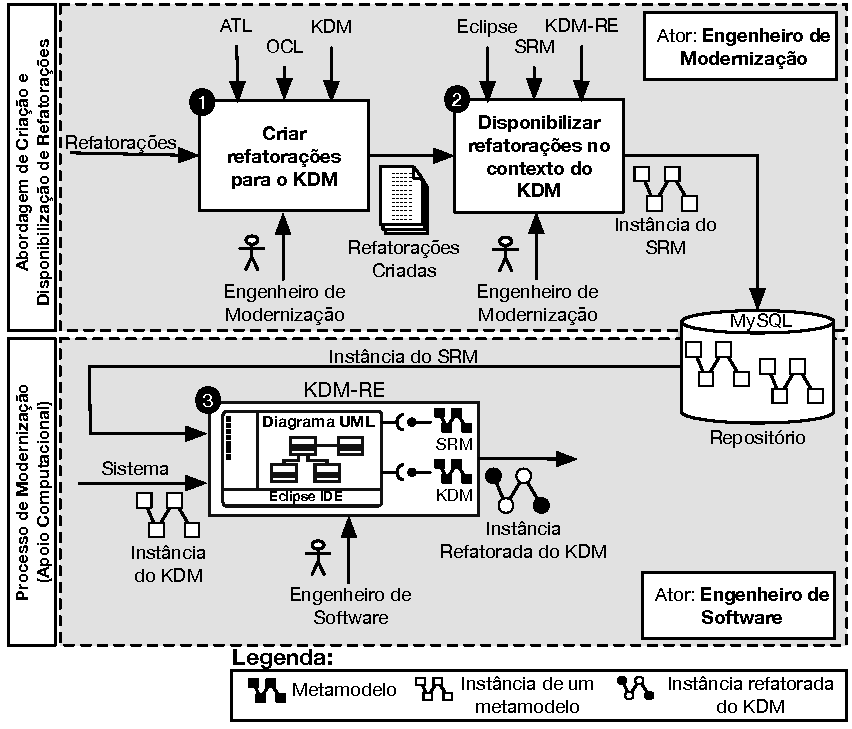
\includegraphics[scale=0.8]{images/NovaFiguraSintexeAbordagem}
	\fautor
\end{figure}


O passo \ding{182} consiste na criação de refatorações para o metamodelo KDM. Esse passo é apoiado por seis diretrizes, as quais o engenheiro de modernização segue para criar refatorações para o metamodelo KDM. As refatorações são um conjunto de regras ATL, as quais são criadas por meio da combinação de um conjunto de artefatos: (\textit{i}) mapeamento entre KDM e POO, (\textit{ii}) operações atômicas, (\textit{iii}) \textit{templates}, (\textit{iv}) linguagem de transformação e (\textit{v}) linguagem de restrição.


% A primeira diretriz consiste em identificar os elementos estruturais entre o paradigma orientado a objeto e o metamodelo KDM. Em seguida, o engenheiro de modernização escolhe qual refatoração almeja criar para o KDM. Então, a refatoração é implementada por meio da linguagem de transformação ATL. As restrições (pré- e pós-condições) da refatoração são implementadas em OCL e o engenheiro de modernização pode documentar a refatoração por meio de duas especificações: informal e formal.


%A criação de refatorações para o KDM é apoiada por cinco diretrizesO objetivo é criar diretrizes para que outros engenheiros de modernização possam criar refatorações para o KDM.

%O metamodelo KDM consiste em um conjunto de pacotes para representar diversos artefatos existentes de um sistema de software. Assim, após a aplicação de refatorações é de suma importância manter todos os pacotes/artefatos sincronizados e consistentes. Dessa forma, no passo \ding{183} regras de propagações são realizadas em instância do metamodelo KDM para manter todos os artefatos sincronizados e consistentes de acordo com a refatoração aplicada. 
%O passo \ding{183} consiste na disponibilização de refatorações por meio de um metamodelo aqui definido. Esse metamodelo contém metaclasses que permitem armazenar informações relacionadas com refatorações, desde seu nome até seu mecanismo. O objetivo é permitir e aumentar a interoperabilidade de refatorações para um amplo domínio e auxiliar o engenheiro de modernização a definir refatorações representativas em forma de metadados. Posteriormente as instâncias desse metamodelo são enviadas para um repositório e são reutilizadas por engenheiros de software por meio de um apoio computacional. O apoio computacional \ding{184} também foi definido para auxiliar o engenheiro de software a aplicar refatorações em sistemas representados pelo KDM. Após a aplicação de refatorações é de suma importância manter todos os pacotes/artefatos sincronizados e consistentes. Dessa forma, esse apoio computacional contém um plug-in responsável por implementar regras de propagações que são realizadas em instância do metamodelo KDM. Essas regras mantêm todos os artefatos sincronizados e consistentes de acordo com a refatoração aplicada. 



O passo \ding{183} consiste na disponibilização das refatorações criadas por meio de um metamodelo aqui definido (\textit{Structured Refactoring Metamodel} - SRM), o qual contém metaclasses que permitem armazenar metadados relacionados com refatorações, tais como: o nome da refatoração, sua motivação, autor, pré- e pós-condições e seu mecanismo. O objetivo desse metamodelo é viabilizar o reúso das refatorações dentro de ferramentas de modernização, propiciando a interoperabilidade entre as mesmas. A instanciação desse metamodelo é apoiada por um apoio computacional criado no contexto desta tese denominado KDM-RE, que fornece uma linguagem específica de domínio para auxiliar o engenheiro de modernização durante a instanciação desse metamodelo. Em seguida, as instâncias desse metamodelo são enviadas pelo KDM-RE para um repositório e podem ser reutilizadas por engenheiros de software. 

%É importante salientar que tanto as restrições (pré- e pós-condições) e os mecanismo das refatorações são disponibilizados no metamodelo por meio de linguagens de transformação (ATL) e restrições (OCL). 

O processo de modernização (ver Figura~\ref{fig:abordagem_kdm_tese_processo} \ding{184}) dá enfoque na aplicação de refatorações e a propagação de mudanças por meio do KDM-RE. KDM-RE foi implementado para automatizar a atividade de aplicação e reutilização de refatorações em sistemas representados pelo KDM. As refatorações podem ser aplicadas diretamente em diagramas de classes UML, porém, a refatoração é de fato realizada transparentemente no metamodelo KDM e, posteriormente, replicada nos diagramas de classes UML. Adicionalmente, após a aplicação de refatorações em sistemas representados pelo KDM, é importante manter todos os pacotes/artefatos sincronizados e consistentes. Dessa forma, o KDM-RE também contém um \textit{plug-in} responsável por aplicar regras de propagações, que são realizadas em instância do metamodelo KDM. O intuito desse \textit{plug-in} é manter todos os artefatos sincronizados e consistentes de acordo com a refatoração aplicada.







%A tese subjacente a este trabalho é de que é possível e benéfico o uso de refatorações para o contexto da ADM, principalmente para o KDM. %Além disso, pretende-se viabilizar a reutilização e padronizações de refatorações por meio da utilização de um metamodelo de refatorações. Adicionalmente, planeja-se verificar a possibilidade de manter todas as visões do metamodelo KDM sincronizada e consistentes após a aplicação de um conjunto de refatorações. %e de técnicas de propagação de mudanças para manter todas as visões do KDM sincronizadas e consistentes após a aplicação de uma refatoração. 
%Neste contexto, esta tese de doutorado cobre os seguintes aspectos: 


%\begin{itemize}
%	\item Definir diretrizes para criar refatorações para o metamodelo KDM;
	
%	\item Criar regras pré-definidas para manter o metamodelo KDM consistente e sincronizado após a aplicar um conjunto de refatorações;
	
%	\item Especificar e criar um metamodelo para auxiliar engenheiros de modernização a compartilhar, criar e reutilizar refatorações no contexto da ADM e KDM;
	%\item a elaboração de uma linguagem específica de domínio (do inglês - \sigla{DSL}{\textit{Domain-Specific Language}}). Essa DSL possui duas finalidades, a saber: (\textit{i}) auxiliar o engenheiro de modernização a instanciar o metamodelo de refatoração proposto e (\textit{ii}) facilitar a criação de um conjunto de refatorações de forma guiada e automática;
	%\item a definição de um ambiente \emph{Web} para também auxiliar a instanciação do metamodelo de refatoração proposto;
	%\item a concepção de um repositório totalmente integrado com a ferramenta %e com o ambiente \emph{web} 
	%para facilitar o compartilhamento e o reúso de refatorações que estão em conformidade com o metamodelo de refatoração proposto.
	
%	\item Elaborar um apoio ferramental totalmente integrado no ambiente de desenvolvimento Eclipse para apoiar a abordagem proposta na Tese.% que possui três módulos: (\textit{i}) módulo de refatoração; (\textit{ii}) módulo do SRM e (\textit{iii})  %com o objetivo de auxiliar o engenheiro de modernização a aplicar, reutilizar e propagar refatorações de forma gráfica, por meio da utilização de diagramas;
%\end{itemize}


%\section{Contribuições}\label{sec:contribuicoes}

%A principal contribuição dessa Tese de doutorado é entender como refatorações tradicionais, ou seja, refatorações comumente utilizadas em sistemas implementados com o paradigma orientado a objeto, podem ser adaptadas, aplicadas, padronizadas e reutilizadas no contexto da ADM e principalmente para o metamodelo KDM. Em outras palavras, esta pesquisa pode ser entendida como uma incursão inicial para auxiliar o OMG e a ADM na definição de padronizações e soluções ferramentais para facilitar o engenheiro de modernização durante o uso de refatorações para o KDM. Pontualmente, pode-se destacar as principais contribuições dessa tese são:

%\begin{itemize}
%	\item Diretrizes para criar e adaptar refatorações para o metamodelo KDM;
%	\item Regras pré-definidas para manter a instância do metamodelo KDM sincronizado e consistente após a aplicação de refatorações;
%	\item Investigação e definição de um metamodelo para auxilar os engenheiros de modernização a criar, compartilhar e reutilizar refatorações no contexto da ADM e KDM;
%	\item Ambiente para auxiliar o engenheiro de modernização durante a aplicação de refatorações para o metamodelo KDM;
%	\item Definição de uma DSL para auxiliar o engenheiro de modernização a instanciar o metamodelo proposto e facilitar a criação de um conjunto de refatorações de forma guiada e automática;
	%\item a elaboração de um ambiente \emph{Web} para também auxiliar a instanciação do metamodelo de refatoração proposto;
%	\item Concepção de um repositório totalmente integrado com a ferramenta para facilitar o compartilhamento e o reúso de refatorações que estão em conformidade com o metamodelo proposto.
%\end{itemize}
    
\section{Convenções Adotadas nesta Tese}\label{sec:convencoes}

Ao longo desta tese, \textit{Itálico} é utilizado para dar ênfases, introduzir novos termos e para destacar palavras em inglês. \texttt{Typewriter} é utilizado para operador Java, operador da DSL, palavras-chaves, nome de metaclasses, meta-associação, meta-atributo, nome de métodos, variáveis e URL que aparecem no texto. Símbolos numéricos (\ding{202}, \ding{203}, \ding{204}, \ding{205}, etc) são usados para chamar a atenção do leitor para informações importantes em figuras e códigos.

\section{Grupo de Pesquisa}

Este trabalho é uma contribuição para o grupo de pesquisa do Departamento de Ciência de Computação e Estatística do Instituto de Ciências Matemáticas e de Computação (ICMC) da Universidade de São Paulo (campus São Carlos/SP). Além disso, a presente pesquisa também foi conduzida em parceria com o grupo de pesquisa AdvanSE (\textit{Advanced Research on Software Engineering}), da Universidade Federal de São Carlos (UFSCar). O grupo possui pesquisas em andamento sobre extensões, refatorações, mineração, métricas e validações de arquitetura utilizando a ADM e o metamodelo KDM, das quais o autor desta tese participa efetivamente.

\section{Estrutura da Tese}

Esta tese está organizada em oito capítulos. No primeiro capítulo, estão apresentados a contextualização, a motivação, a abordagem desenvolvida em resumo, os objetivos, as convenções adotadas e o grupo de pesquisa do trabalho. 

No Capítulo~\ref{chapter:fundamentacao_teorica}, estrutura-se uma revisão dos principais conceitos envolvendo MDE e refatoração com o objetivo de facilitar a compreensão  com relação à tese. Além disso, é feita uma contextualização sobre a modernização de sistemas com a utilização dos padrões propostos pelo OMG, ADM e KDM, em que seus conceitos e particularidades são observados. Também é apresentada a ferramenta MoDisco. 
%
%No Capítulo~\ref{chapter:adm_kdm} é ilustrada uma contextualização sobre a modernização de sistemas com a utilização dos padrões propostos pelo OMG, ADM e KDM, em que seus conceitos e particularidades são observados. Também é apresentada a ferramenta MoDisco, utilizada nesta Tese. 
%
No Capítulo~\ref{chapter:mapeamento_sistematico}, é apresentado um mapeamento sistemático que foi realizado com o objetivo de identificar e entender soluções já desenvolvidas sobre ADM e KDM. Além disso, nesse mapeamento também são demonstradas as principais constatações e questões em aberto que nortearam a tese.

Como descrito na Figura~\ref{fig:abordagem_kdm_tese_processo}, a abordagem aqui proposta contém três passos. O passo \ding{182} é apresentado no Capítulo~\ref{chapter:catalogo_refactoring_KDM}, onde são destacadas as diretrizes para criar refatorações para o metamodelo KDM. O passo \ding{183} é salientado no Capítulo~\ref{chapter:Toward_a_Refactoring_Metamodel_for_KDM}, o qual apresenta um metamodelo para disponibilizar e promover o reúso de refatorações no contexto da ADM e KDM. %No Capítulo~\ref{chapter:Abordagem_de_sincronizacao} é apresentada uma abordagem denominada KDM-SInc que é utilizada para manter uma determinada instância do metamodelo KDM consistente e sincronizado após a aplicação de refatorações. 
%
O passo~\ding{184} é alicerçado por um apoio computacional, o qual é apresentado no Capítulo~\ref{chapter:ferramenta_kdm_re}. Esse apoio computacional é denominado KDM-RE e é composto por três \textit{plug-ins} do Eclipse: (\textit{i}) o primeiro consiste em um conjunto de \textit{Wizards} que apoia o engenheiro de software na aplicação das refatorações em diagramas de classe UML; (\textit{ii}) o segundo consiste em um apoio à importação e reúso de refatorações disponíveis no repositório; (\textit{iii}) o terceiro consiste em um módulo de propagação de mudanças que permite manter modelos internos do KDM sincronizados.


No Capítulo~\ref{chapter:avaliacao}, é mostrado o planejamento, execução e análise dos dados de um experimento que visa validar a abordagem desenvolvida nesta tese. E, por fim, no Capítulo~\ref{chapter:conclusoes}, são descritas as conclusões do trabalho com as principais contribuições, limitações, lições apreendidas, publicações e trabalhos futuros que poderão ser conduzidos como continuação da presente pesquisa.

%No Capítulo~\ref{chapter:avaliacao}, é mostrado o planejamento, execução e análise dos dados de dois experimentos \unsure{ver} que visaram validar a abordagem desenvolvida nesta tese.  E, por fim, no Capítulo~\ref{chapter:conclusoes}, são descritas as conclusões do trabalho com as principais contribuições, limitações, lições apreendidas, publicações e trabalhos futuros que poderão ser conduzidos como continuação da presente pesquisa.


%A Tese está estruturada de acordo com a Figura~\ref{fig:structure_these_not_final}

%\begin{figure}[h]
%	\centering
	% Requires \usepackage{graphicx}
	%\caption{Macro visão da abordagem proprosta.}
	%\label{fig:abordagem_kdm_tese_processo}
	%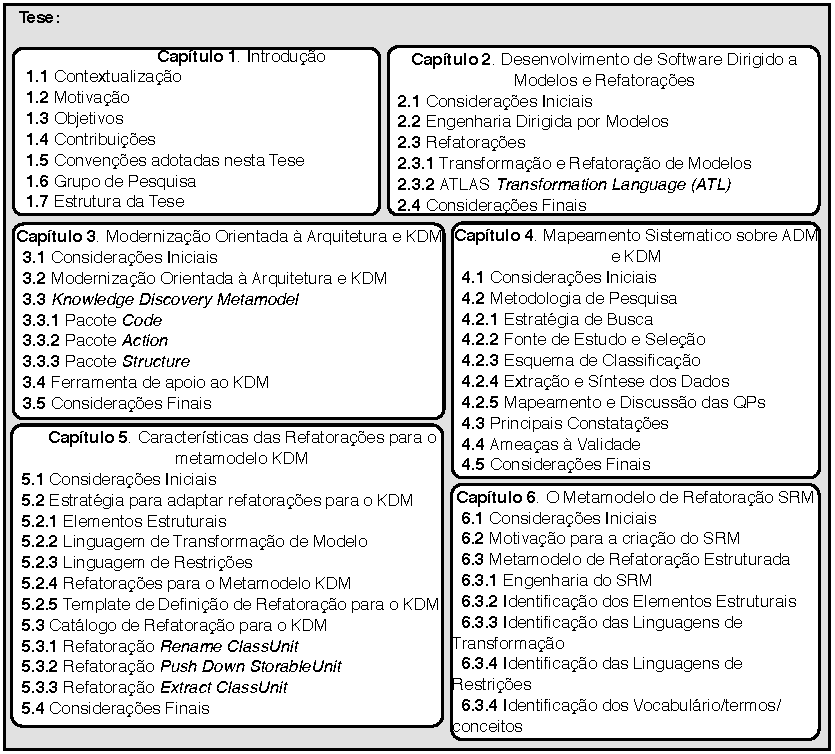
\includegraphics[scale=0.9]{images/PhD_Structure_Figure}
	%\fautor
%\end{figure}

\chapter{Fundamentação Teórica}
\label{chapter:fundamentacao_teorica}

\section{Considerações Iniciais}

Neste capítulo são apresentados e discutidos os conceitos fundamentais para o entendimento desta Tese. Ele está organizado da seguinte forma: na Seção~\ref{Cap2_Sec2_Desenvolvimento_Dirigido_a_Modelos}, os conceitos sobre Engenharia Dirigido por Modelos são salientados; na Seção~\ref{sec:refatoracao} são definidos os conceitos sobre refatoração, bem como refatorações para modelos. Na Seção~\ref{sec:modernizacaoOrientada_Arquitetura} é feita uma contextualização sobre a Modernização Dirigida a Arquitetura; na Seção~\ref{sec:knowledge_discovery_meta_model} o metamodelo KDM é apresentado; na Subseção~\ref{subsection:codePackage} é descrito o pacote \texttt{Code}; na Subseção~\ref{sec:actionPackage} é descrito o pacote \texttt{Action}; na Subseção~\ref{sec:structurePackage} é apresentado o pacote \texttt{Structure}; na Seção~\ref{sec:Ferramenta_de_apoio_KDM_capitulo} é mostrada uma ferramenta de apoio ao KDM e em seguida na Seção~\ref{capitulobaclCOnsideracoesFinais} as considerações finais deste capítulo são destacadas.

\section{Engenharia Dirigida por Modelos}\label{Cap2_Sec2_Desenvolvimento_Dirigido_a_Modelos}

De acordo com~\citeonline{Booch:2004:OAD:975416} modelos são abstrações de sistemas que permitem raciocinar e entender o sistema, ignorando detalhes irrelevantes no modelo, enquanto focalizamos nos detalhes mais relevantes. Segundo~\citeonline{Brown_2007, Bezivin02apreliminary}, a utilização de modelos para o desenvolvimento de software não é algo novo. Modelos estão sendo usados há algumas décadas para auxiliar a  concepção e projeto de software, sendo utilizados basicamente nas fases iniciais do desenvolvimento. Por exemplo, modelos como os da UML~\cite{UML:OMG} não fazem parte do software em si, embora sejam importantes para o entendimento e a construção. Os desenvolvedores os criam, mas os descartam, implementando as funções de forma manual e realizando manutenções somente no código-fonte. Desse modo, o conhecimento acerca da solução fica criptografado no código-fonte e dificilmente é reutilizado. Portanto, há necessidade de criar modelos que representem esse conhecimento e que possam ser úteis tanto para a documentação quanto para a construção e manutenção de software.


A partir dessa ideia, a \textit{Model-Driven Engineering} (MDE) surge como uma solução complementar aos processos de desenvolvimento tradicionais~\cite{Lima_2007}. A MDE é uma abordagem que propõe reduzir a distância semântica entre o problema do domínio e a solução/implementação. Nessa abordagem, o desenvolvimento de software ocorre por meio de modelos que protegem os desenvolvedores das complexidades da implementação e de transformações que originam o código-fonte de maneira automatizada a partir das informações contidas nesses modelos. Na literatura é possível também identificar MDE como outros acrônimos, por exemplo, \sigla{MDD}{\textit{Model-Driven Development}}, \sigla{MDSD}{\textit{Model-Driven Software Development}} ou MD*~\cite{Kleppe:2003}, todos esses acrônimos dizem respeito à mesma abordagem. O que é importante ter em mente sobre MDE é que modelos são utilizados no centro do processo de desenvolvimento e manutenção de software. Na MDE, os modelos assumem o papel principal em todo o ciclo de vida de um software. A relevância dos modelos vai além da documentação do software desenvolvido. Na MDE modelos passam a ser utilizados como artefatos principais; eles podem ser compreendidos por computadores e são fundamentais para o desenvolvimento do software, pois podem ser manipulados, refinados e transformados para uma nova versão, até que a partir deles é gerado o código-fonte~\cite{Kleppe:2003, Brown_2007, Ben_Ammar}.

Na MDE o enfoque do desenvolvimento é direcionado aos modelos, ou seja, a modelagem deixa de ser meramente uma forma de planejar o código e passa a ser uma forma de construir o software. O nível de abstração da programação torna-se mais elevado, reduzindo necessidade do desenvolvedor de interagir manualmente com o código-fonte~\cite{Braganca_Machado}. A MDE não tem como objetivo substituir o processo tradicional de desenvolvimento de software~\cite{Kleppe:2003, Brown_2007, Braganca_Machado} e sim contribuir para o seu aprimoramento. O OMG~\cite{ADM:OMG} definiu um modelo de arquitetura para o MDE, conhecido como \emph{Model-Driven Architecture} (MDA). MDA tem como objetivo promover o uso de modelos no desenvolvimento de software, para fornecer uma solução ao gerenciamento da complexidade do desenvolvimento, manutenção e evolução de sistemas de software e favorecer a interoperabilidade e portabilidade desses sistemas.

O OMG definiu formalmente a MDA como uma abordagem que é bem definida pela ideia de separar a especificação das operações de um sistema dos detalhes de como este sistema usa as potencialidades de sua plataforma. Isso possibilita que ferramentas ofereçam a especificação de um sistema de forma independente de plataforma. De acordo com o OMG os principais objetivos da MDA são a portabilidade, a interoperabilidade e a reusabilidade. Para alcançar esses objetivos a MDA divide o desenvolvimento de software em níveis de abstração~\cite{France_2007, Ben_Ammar}, os níveis são:

\begin{itemize}
	\item Modelo Independente de Computação (do inglês - \sigla{CIM}{\emph{Computation Independent Model}}): descreve o negócio, ou ambiente, no qual o software irá operar. Como a decisão a respeito da informatização é feita por uma pessoa e não por uma ferramenta de transformação, dificilmente a transformação automatizada desse modelo para o de nível seguinte é implementada;
	\item Modelo Independente de Plataforma (do inglês - \sigla{PIM}{\emph{Platform Independent Model}}): nível de análise, em que ocorre a definição das características do software ou domínio. Esse modelo pode ser transformado para um ou mais modelos do nível seguinte;
	\item Modelo Específico de Plataforma (do inglês - \sigla{PSM}{\textit{Platform Specific Model}}): nível de projeto, considera as tecnologias de implementação, devendo existir uma instância desse modelo para cada plataforma de implantação do software. A partir desse modelo ocorre a transformação para o código-fonte.
\end{itemize}

Com base nos princípios mencionados, pode-se citar as seguintes vantagens da MD*~\cite{Hutchinson_2011, France_2007, Schmidt_2006}:

\begin{enumerate}
	\item Maior facilidade na criação dos modelos das aplicações, pois é utilizada uma linguagem de específica para o domínio do problema;
	\item Maior produtividade e redução do esforço dos desenvolvedores, pois a maior parte do código-fonte das aplicações pode ser gerado a partir dos modelos;
	\item Maximização do tempo de vida útil dos modelos e de outros artefatos, pois como são necessários para a geração de código, eles são menos propensos a serem descartados pelos desenvolvedores nos processos de manutenção;
	\item Flexibilidade de desenvolvimento, pois os modelos independentes de plataforma armazenam a lógica do sistema e são menos sensíveis a essas mudanças;
	\item O conhecimento a respeito do software não fica exclusivamente na mente dos desenvolvedores e no código, fazendo com que os processos de desenvolvimento e de manutenção fiquem menos vulneráveis às oscilações de pessoal.
\end{enumerate}

A MD* não pretende substituir os processos tradicionais de desenvolvimento de software e sim contribuir para seu aprimoramento, porém, de uma maneira racional para mover informações de uma fase de desenvolvimento para outra, trazendo respostas rápidas e eficientes para atender as necessidades inesperadas de novos requisitos.

De acordo com~\citeonline{Kleppe:2003}, um modelo deve ser definido como uma descrição de um (ou de uma parte) sistema expresso em uma linguagem bem definida, isto é, respeitando uma sintaxe e uma semântica. Esta descrição deve ser conveniente para uma interpretação automatizada por computadores. Assim, para criar um modelo deve-se seguir uma sintaxe precisa e uma semântica bem definida a fim de regulamentar a criação de elementos e suas relações. Em MDE esse formalismo pode ser alcançado utilizando uma linguagem de modelagem. Tais linguagens são especificações que contêm os elementos bases para construir modelos, concebida dentro de um domínio limitado e com objetivos específicos. Usualmente uma linguagem de modelagem pode ser gráfica ou textual com notação matemática e deve permitir a definição de modelos sem ambiguidades. O uso de uma linguagem bem definida sintaticamente e semanticamente permite o entendimento e manipulação de modelos por pessoas e computações~\cite{Hutchinson_2011, France_2007, Schmidt_2006}.

Uma linguagem de modelagem geralmente está em conformidade com um metamodelo. Um metamodelo é um modelo que define uma linguagem para representar um modelo. A linguagem de modelagem é simplesmente um modelo do metamodelo. Ela define a estrutura, a semântica e as restrições para uma família de modelos~\cite{Mellor_2004}. Na Figura~\ref{fig:metamodelosCamadas} é apresentado os quatro níveis de modelos da MDE. Note que as relações entre os níveis descritos na Figura~\ref{fig:metamodelosCamadas} são do tipo \aspas{\texttt{instance of}} (instância de) definido por~\citeonline{Bezivin02apreliminary, Brambilla_2012}. Os quatros níveis são descritos a seguir: 

\begin{figure}[htb]
 \caption{Arquitetura de Metamodelagem.}
 \label{fig:metamodelosCamadas}
 \centering
 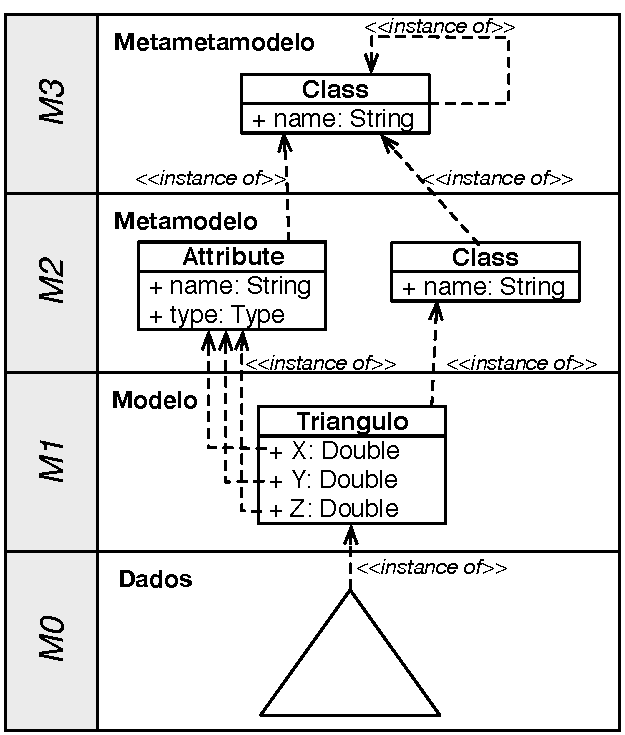
\includegraphics[scale=0.9]{images/Arquitetura_de_metamodelagem}
 \fautor
\end{figure}

\begin{itemize}
	\item metametamodelo (M3): M3 constitui a base da arquitetura de meta-modelagem. A função primordial deste nível é definir linguagens para especificar metamodelos. Um meta-metamodelo define um modelo de mais alto nível de abstração que o metamodelo, e este primeiro é tipicamente mais compacto que o segundo. \textit{Meta-Object Facility} (MOF)~\cite{MOF} é \sigla{EMF}{\emph{Eclipse-Modeling Framework}}\cite{EMF} são exemplos de meta-metamodelos;
	\item metamodelo (M2): um metamodelo representa uma instância de um meta-metamodelo. A função principal do nível do metamodelo é definir uma linguagem para especificar modelos. Os metamodelos são tipicamente mais elaborados que os meta-metamodelos. Por exemplo, a UML~\cite{UML:OMG} e o KDM~\cite{KDM:ISO} ambos possuem metamodelos que os descrevem estruturalmente;
	\item modelo (M1): um modelo é uma instancia de um metamodelo. A função principal do nível de modelo é definir uma linguagem para descrever um domínio específico;
	\item dados (M0): os objetos de usuários representam os dados finais. A principal responsabilidade dos objetos de usuários é descrever um domínio específico em uma plataforma final.
\end{itemize}

Um objetivo claro da MDA é fornecer um \textit{framework} que integra os padrões existentes do OMG. Os principais padrões do OMG utilizados nesta Tese são:

\begin{itemize}
\item \textit{Meta Object Facility} (MOF): Linguagem abstrata e um \textit{framework} para especificação, construção e gerenciamento de metamodelos independentes de plataforma. Essa especificação contém um conjunto de construtores que é utilizado para a definição de metamodelos. MOF pode ser utilizado para definir outras linguagens;
\item \sigla{UML}{\textit{Unified Modeling Language}}: É uma linguagem para especificação, construção, visualização e documentação de artefatos de software. Essa linguagem permite a modelagem de diferentes aspectos ou pontos de vista de um sistema;
\item \textit{Knowledge Discovery Metamodel} (KDM): Metamodelo utilizado para representar em nível de modelos artefatos de sistemas de software. Capítulo~\ref{chapter:adm_kdm} maiores informações sobre esse metamodelo, bem como suas metaclasses são apresentadas;
\item \textit{XML Metadata Interchange} (XMI): Padrão do OMG para troca de informação baseado em \sigla{XML}{\textit{eXtensible Markup Language}}. Pode ser utilizado para trocar qualquer informação cujo metamodelo pode ser expresso utilizando MOF. O uso mais comum da XMI é como um formato de intercâmbio de modelos UML, embora também possa ser utilizado para a serialização de modelos de outras linguagens;
\item \textit{ATL Transformation Language} (ATL): É uma implementação da \textit{Query/View/Transformation} (QVT) que é uma especificação híbrida padronizada para transformação de modelos no contexto de metamodelagem MOF. ATL aceita construções declarativas e imperativas, ver Subseção~\ref{sub:atl_transformation_language};
\sigla{OCL}{\textit{Object Constratint Language}}: É uma linguagem declarativa para descrever regras que se aplicam aos modelos. A OCL, inicialmente, era apenas uma extensão da UML para especificações formais de modelos. Hoje em dia, a OCL pode ser utilizada para especificar pré- e pós-condições, podendo ser utilizada em qualquer modelo cujo metamodelo seja MOF.
\end{itemize}

\section{Refatoração}\label{sec:refatoracao}

Refatoração pode ser entendida como um processo de redistribuição de funcionalidade com o intuito de melhorar um dado sistema. No contexto do paradigma orientado a objeto, essa redistribuição está totalmente ligada com classes, atributos e operações. A refatoração tem como objetivo permitir a redistribuição de classes, atributos e operações na hierarquia de classes para facilitar futuras atividades de desenvolvimento ou de manutenção. A primeira definição de refatoração foi concebida por~\citeonline{OPDYKE_1992} da seguinte forma: \aspas{refatorações são transformações que reestruturam um determinado sistema com o objetivo de melhorar o \textit{design}, evolução e reuso de sistemas desenvolvidos no paradigma orientada a objeto}.

No contexto do paradigma orientado a objeto, refatoração é uma alternativa do conceito de reestruturação. Em outras palavras, refatoração é um termo aplicado ao paradigma orientado a objeto; para outros paradigmas de programação, esse mesmo processo é descrito como reestruturação~\cite{Chikofsky_cross}. De acordo com~\citeonline{Chikofsky_cross}, reestruturação \aspas{consiste no processo de alterar um software, melhorando a sua estrutura interna, de forma que o comportamento externo do código não seja alterado}. Reestruturação e refatoração são técnicas essenciais que são utilizadas para mitigar problemas relacionados à evolução de software~\cite{OPDYKE_1992}. Com o objetivo de aumentar atributos de qualidade dos sistemas, as práticas de refatoração surgiram através do emprego de reestruturação sobre unidades de código preservando o seu comportamento~\cite{Chikofsky_cross,OPDYKE_1992}.

Quando aplicada durante a fase de manutenção de software, a refatoração ajuda a tornar o código mais legível e também tem como objetivo solucionar problemas de códigos mal escritos~\cite{Chikofsky_cross}. A refatoração também pode ser usada no contexto da reengenharia a fim de alterar um sistema específico visando reconstruí-lo em um novo formato. Nesse contexto, a refatoração é necessária para converter código legado ou deteriorado em um formato mais estruturado ou modular, ou para migrar o código para uma diferente linguagem de programação, ou mesmo um diferente paradigma de linguagem.

Em seu livro,~\citeonline{Fowler1999}, apresenta duas definições para refatoração, uma como substantivo e outra como verbo:

\begin{itemize}
	\item Refatoração: uma mudança que é realizada na estrutura interna de um determinado sistema com o objetivo de deixar o sistema mais fácil de entender e fácil de modificar sem alterar o seu comportamento externo; e
	\item Refatorar: reestruturar o software por meio de um conjunto de refatorações sem modificar o seu comportamento externo.
\end{itemize}

As definições apresentadas por~\citeonline{Fowler1999} enfatizam que o propósito da refatoração é fazer com que o software fique mais fácil de entender (melhorar sua compreensão) e de modificar (melhorar sua manutenibilidade). Outra característica de suma importância a ser destacada é que a refatoração em geral deve ser um processo para melhorar o \textit{design} do software. De acordo com~\citeonline{Wake_2003} , refatoração é \aspas{uma arte para melhorar cuidadosamente o \textit{design} de códigos existentes.} O autor também enfatiza que refatoração deve fornecer maneiras de identificar problemas no código e também deve prover soluções para corrigir tais problemas.~\citeonline{Wake_2003} caracteriza refatoração como:

\begin{itemize}
	\item refatoração não inclui nenhuma mudança no sistema - refatoração não deve adicionar novas funcionalidades ao sistema;
	\item refatoração deve ser utilizada para melhorar o código do sistema;
	\item nem toda reestruturação pode ser considerada como refatoração - usualmente refatorações tendem a ser transformações pequenas e seguras. 
\end{itemize}

O primeiro conjunto de refatorações foi proposto por~\citeonline{OPDYKE_1992}, onde o autor definiu 26 refatorações de baixa granularidade. Tais refatorações podem ser resumidas da seguinte forma:

\begin{itemize}
	\item criar um membro  - variável/função/classe: Essas refatorações tem como objetivo criar novas variáveis e/ou funções para uma classe em particular ou criar um nova classe;
	\item deletar um membro - variável/função/classe. Essas refatorações têm como objetivo  deletar membros que não estão sendo utilizados;
	\item renomear um membro - variável/função/classe. Essas refatorações podem ser utilizadas pare renomear membros e fornecerem nomes mais significativos;
	\item mover um membro - variável/função. Essas refatorações são utilizadas para redistribuir um conjunto de variáveis/funções para sub ou superclasses.
\end{itemize}

Similarmente,~\citeonline{Roberts_1999} definiu um conjunto de refatorações que devem ser aplicadas em classes, métodos e atributos. Porém o catálogo mais completo e extensivo de refatorações foi definido por~\citeonline{Fowler1999}. Neste catálogo cada refatoração possui os seguintes tópicos: (\textit{i}) um nome, (\textit{ii}) uma breve descrição, (\textit{iii}) uma motivação para a condução da refatoração, (\textit{iv}) um mecanismo descrevendo como a refatoração deve ser executada e (\textit{v}) um exemplo ilustrando a utilização da refatoração. As refatorações proposta por~\citeonline{Fowler1999} são agrupadas em setes categorias, a saber: (\textit{i}) \textit{Composing Methods}, (\textit{ii}) \textit{Moving Features Between Objects}, (\textit{iii}) \textit{Organizing Data}, (\textit{iv}) \textit{Simplifying Conditional Expressions}, (\textit{v}) \textit{Make Method Calls Simpler}, (\textit{vi}) \textit{Dealing with Generalization} e (\textit{vii}) \textit{Big Refactorings}.

De acordo com~\citeonline{Fowler1999} existem quatro principais motivações para a aplicação de refatoração:

\begin{enumerate}
	\item refatorações quando bem conduzidas tendem a melhorar o \textit{design} do software - dessa forma, refatoração pode auxiliar na prevenção da decadência do software e eliminando código duplicado;
	\item refatorações fazem com que o código-fonte fique mais fácil de entender - código bem legível facilita a comunicação e seu propósito;
	\item refatoração auxilia na identificação de erros - melhorando a estrutura interna do código-fonte erros tendem a ser identificados mais facilmente;
	\item desenvolvimento mais produtivo - uma boa estrutura interna usualmente facilita o desenvolvimento e melhora a produtividade.
\end{enumerate}

Como já salientado refatorações devem preservar o comportamento de um determinado software após a aplicação de \textit{n} refatorações. Dessa forma,~\citeonline{Mens04,Cinneide_2000} relatam que existem três principais abordagens para auxiliar a preservação (de alguns aspectos) do comportamento do código-fonte. Tais abordagens são: (\textit{i}) abordagem não formal (por exemplo, as refatorações definidas por~\citeonline{Fowler1999}), (\textit{ii}) uma abordagem semiformal~\cite{Roberts_1999} e (\textit{iii}) abordagem completamente formal. No entanto, os autores também argumentam que mesmo com a utilização da última abordagem é impossível garantir totalmente a preservação de comportamento após a aplicação de refatorações~\cite{Mens04,Cinneide_2000}. 

A ideia de preservação de comportamento no contexto de refatoração foi primeiramente introduzida por~\citeonline{OPDYKE_1992} da seguinte forma: \aspas{Se um programa é chamado duas vezes (antes e depois da refatoração) com o mesmo conjunto de entradas, o resultado deve ser o mesmo}. Essa explicação é plausível e utilizada na literatura~\cite{Roberts_1999, Fowler1999}, mas infelizmente não é suficiente. Por exemplo, considere o seguinte cenário. Se uma classe, um método ou outra estrutura de código é renomeada utilizando a refatoração \texttt{Rename} é desejado que todas as  declarações e utilizações correspondentes também sejam atualizadas. No entanto, suponha o Código-fonte~\ref{lst:example_refactoring_behavior}, se a classe \texttt{Foo} é renomeada para \texttt{Bar} o comportamento do programa é alterado: o Código-fonte~\ref{lst:example_refactoring_behavior} não irá imprimir \aspas{Foo} e sim \aspas{Bar}. Dessa forma, a definição apresentada por~\citeonline{OPDYKE_1992} não é verdadeira para esse cenário.   

\begin{codigo}[caption={[Um simples programa ilustrando porque é errado acreditar que refatoração não muda a saída de um programa.] Simples exemplo do efeito de uma refatoração.},escapeinside={(*@}{@*)}, basicstyle=\footnotesize, language=java, label={lst:example_refactoring_behavior}]{Name}
	public class Foo {
	    public void method(){
	        String className = this.getClass().getName();
	        System.out.println(className);
	    }
	}
\end{codigo}

Outra abordagem para a definição de comportamento é exigir a preservação sintática e semântica de um sistema após a aplicação de refatorações. Obviamente uma refatoração por definição não deveria invalidar a sintaxe de um sistema. Usualmente, a sintaxe e semântica são preservadas por meio de asserções. Asserção é definida por meio de pré- e pós-condições que são executadas antes e após a aplicação de uma refatoração. Pré-condições são asserções que um sistema deve satisfazer para que a refatoração possa ser aplicada de forma segura. Pré-condições podem ser pensadas como condições que caracterizam válidas transformações. Por exemplo, uma possível pré-condição para a refatoração \texttt{Rename Class} seria verificar se o novo nome da classe já existe dentro do pacote que a classe esta definida. ~\citeonline{OPDYKE_1992} foi o primeiro pesquisador a utilizar asserções para garantir que as refatorações aplicadas preservavam a sintaxe e a semântica dos sistemas. É importante observar que as  refatorações apresentadas nesta Tese para o metamodelo KDM foram propostas e adaptadas com o intuito de preservar a sintaxe e semântica do sistema. O metamodelo KDM provê meios de garantir que a estrutura do código-fonte foi preservada utilizando o pacote \texttt{Code} e \texttt{Action}.

O processo para a aplicação de um refatoração contém três principais passos~\cite{Wake_2003}. O primeiro passo consiste na identificação de partes do código que precisam ser refatoradas. O segundo passo consiste na escolha da melhor refatoração para solucionar o problema anteriormente identificado. O terceiro passo consiste na aplicação da refatoração. Seguindo a mesma ideologia e fundamentação proposta por~\citeonline{Fowler1999} e~\citeonline{OPDYKE_1992} existe a possibilidade de aplicar refatorações para modelos. Na subseção a seguir os conceitos e características relacionados com refatorações para modelos são apresentados.


% subsection modelos_e_meta_modelos (end)
\subsection{Transformação e Refatoração de Modelos}\label{sec:transformacoes_de_modelos}

Refatorações para modelos são transformação de modelos\footnote{Transformação e Refatoração de modelos são utilizadas nesta Tese de forma intercambiáveis.} que têm como principal objetivo melhorar a estrutura do modelo e também preservar suas características internas. Refatorações para modelos é uma área de estudo relativamente nova quando comparada com refatorações tradicionais, ou seja, aquelas aplicadas em código-fonte. De acordo com a literatura, refatorações para modelos é uma área mais desafiadora do que refatorações tradicionais, uma vez que modelos usualmente possuem múltiplas visões que precisam permanecer sincronizados e consistentes após a aplicação de refatorações. Por exemplo, na literatura é possível identificar trabalhos que apresentam o estado da arte~\cite{Tom_2008_2008}, taxonomias~\cite{Maddeh_2010} e desafios~\cite{mens_03_refactoring, Mens07RefacTools, Van_Der_Straeten_2009, mens2003refactoring_novo_rafa} em relação à refatorações para modelos. 

Tais autores afirmam que a transformação em modelo desempenha um papel fundamental em abordagens que utilizam os princípios de MDE, pois permite a manipulação de modelo de forma totalmente automática. Uma transformação consiste na geração automática de um modelo alvo tendo como base um modelo fonte, sendo que essa transformação é definida por meio de um conjunto de regras de transformações~\cite{Mens_2006}. 

Nos trabalhos de~\citeonline{Mens_2006, Czarnecki_2006} e ~\citeonline{Biehl_2010} os autores buscam identificar e classificar as transformações de modelos. Algumas das classificações apresentadas por tais autores são citadas de forma resumida, a seguir:

\begin{itemize}
	\item Vertical ou Horizontal: Os modelos fonte e alvo podem estar em um ou mais níveis de abstração. Uma transformação horizontal mantém modelos fonte e alvos no mesmo nível de abstração. Na transformação vertical, existe uma mudança de nível de abstração nos modelos. Esta mudança pode ser tanto para aumentar quanto par diminuir o nível de abstração;
	\item  Endógenas ou Exógenas: Nas transformações Endógenas os modelos envolvidos são expressos na mesma linguagem de modelagem. Nas transformações Exógenas os modelos que participam da transformação são de linguagens diferentes;
	\item Bidirecionais: Uma transformação bidirecional pode tanto gerar modelos alvos utilizando como base modelos fontes, quanto gerar modelos fontes utilizando modelos alvos. Em contrapartida, transformação unidirecional existe apenas um fluxo de execução. 
\end{itemize}

As transformações do tipo classificadas como endógenas ou exógenas~\cite{Brambilla_2012} são apresentadas na Figura~\ref{fig:model_transformations}. Como pode ser observado na Figura~\ref{fig:model_transformations} transformações em modelos do tipo endógenas apenas um modelo e um metamodelo são utilizados, por outro lado, transformações do tipo exógenas os metamodelos alvo e fonte são diferentes. Usualmente, refatorações em modelo são um exemplo de transformações do tipo endógenas, e uma transformação que tem como objetivo transformar uma linguagem para uma outra linguagem é um exemplo de transformações do tipo exógenas. Transformações em modelos que utilizam apenas um modelo como entrada e geram o mesmo modelo como saída com algumas modificações, essas transformações são classificadas como \aspas{\emph{in-place}}, enquanto que transformações em modelos que utilizam como entrada um modelo e tem como objetivo gerar um outro modelo como saída são consideradas \aspas{\emph{out-place}}. 

Transformações endógenas são mais interessantes quando apenas um subconjunto do modelo será afetado pela transformação~\cite{Brambilla_2012}. Por exemplo, em um editor de modelos transformações endógenas podem ser utilizadas para definir pequenas mudanças para automatizar tarefas repetitivas durante o desenvolvimento de modelos. Outra aplicação interessante de transformações endógenas é a condução de refatoração em nível de modelos. Um dos principais objetivos dessa Tese de doutorado são a criação e utilização de refatoração em modelos, assim, maior ênfase será concentrada em transformações de modelos do tipo endógenas no restante dessa subseção.


\begin{figure}[ht]
\centering
\caption{Diferentes tipos de transformações em modelos.}
\subfigure[\emph{exogenous} \aspas{\emph{out-place}}]{%
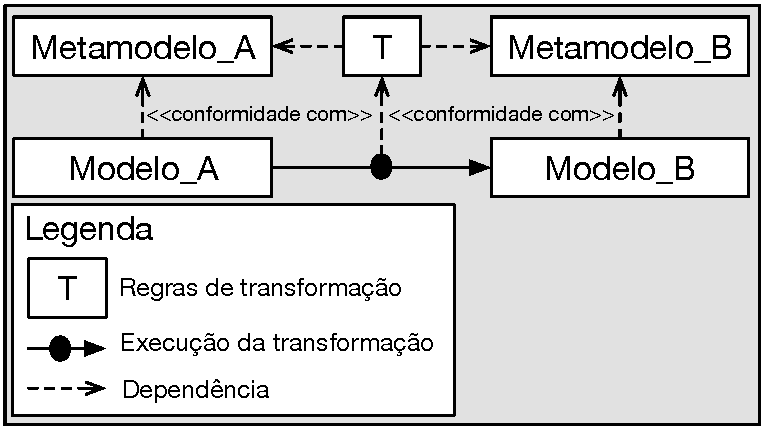
\includegraphics[scale=0.7]{images/transformacaoModeloA}
\label{fig:subfigure1}}
\quad
\subfigure[ \emph{endogenous} \aspas{\emph{in-place}}]{%
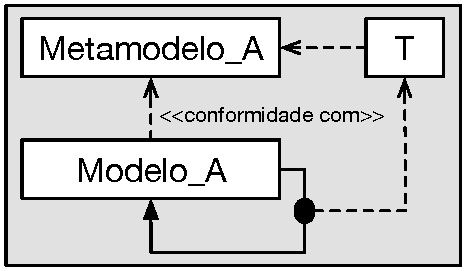
\includegraphics[scale=0.7]{images/transformacaoModeloB}
\label{fig:subfigure2}}
\label{fig:model_transformations}
 \fadaptada{Brambilla_2012}
\end{figure}

%\begin{figure}[htb]
% \caption{Diferentes tipos de transformações em modelos: (a) \emph{exogenous} \aspas{\emph{out-place}} vs. (b) \emph{endogenous} \aspas{\emph{in-place}}}
% \label{fig:model_transformations}
% \centering
% 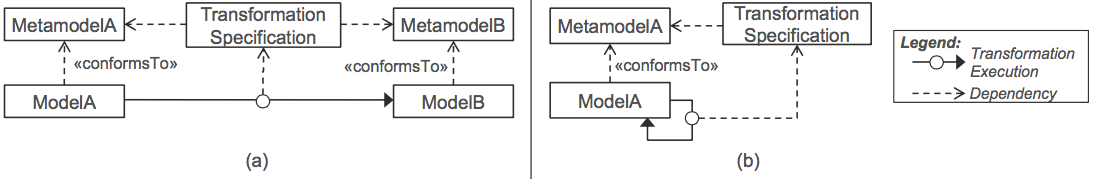
\includegraphics[scale=0.45]{images/transformacoes.png}
% \fadaptada{Brambilla_2012}
%\end{figure}

Transformações endógenas usualmente são implementadas utilizando técnicas de \aspas{reescrita de grafo}, ou como também é conhecido \aspas{transformação de grafo}~\cite{Ehrig_2006}. Na teoria dos grafos, \aspas{reescrita de grafo} é um conjunto de regras para reescrever um determinado grafo, por exemplo, dado $p: \emph{left-hand side} (LHS) \rightarrow \emph{right-hand side} (RHS)$, sendo $LHS$ o grafo usado como padrão (no lado esquerdo) e $RHS$ o grafo de substituição (no lado direito da regra). Mais precisamente, o lado esquerdo, LHS, representa todas às pré-condições que devem ser satisfeitas antes da execução das regras de transformações. Similarmente, o lado direito, RHS, contém todas as pós-condições. As ações que serão executadas pelas regras de transformações são implicitamente definidas tanto no grafo LHS quanto no grafo RHS. A execução de um conjunto de regra de transformação produz os seguintes efeitos: (\textit{i}) todos os elementos que apenas estão contidos no grafo LHS são deletados; (\textit{ii}) todos os elementos que apenas estão contidos no grafo RHS são adicionados; e (\textit{iii}) todos os elementos que estão contidos em ambos os grafos, LHS e RHS, são preservados~\cite{Ehrig_2006}. 

Neste contexto, \aspas{reescrita de grafo} é útil para auxiliar na definição de transformações de modelos e metamodelos. Por exemplo, de acordo com~\citeonline{Lehnert_2012, Fluri_2006}, técnicas de \aspas{reescrita de grafo} podem ser aplicadas em qualquer metamodelo e modelos que implementam o padrão MOF, ou seja, KDM, UML, entre outros. Qualquer instância de um metamodelo que implemente o padrão MOF pode ser representado como um grafo da seguinte forma: (\textit{i}) vertices podem ser entendidos como: \texttt{EPackage}, \texttt{EClass}, \texttt{EDataType}, \texttt{EEnum}, \texttt{EAnotation}, \texttt{EOperation}, \texttt{EAttribute} e \texttt{EEnumLiteral}; (\textit{ii}) arestas pode ser representadas em metamodelo como: \texttt{EReference}, \texttt{Inheritance}, \texttt{EAnnotationLink}. Assim, pode-se definir e realizar evoluções, simulações, refatorações de modelos por meio de técnicas de \aspas{reescrita de grafo}. 

% Dessa forma, as gramáticas de um grafo consistem de um conjunto de regras de transformações e um grafo inicial (geralmente referenciado como grafo \aspas{hospedeiro}) onde as regras de transformações são aplicadas. Usualmente as regras de transformações consistem de um grafo denominado \emph{left-hand side} (LHS) e um grafo \emph{right-hand side} (RHS). O grafo LHS tem como intuito representar todas as pré-condições para antes do conjunto de regras de transformações serem aplicadas no modelos. Similarmente, o grafo RHS contêm todas as pós-condições. As ações que serão executadas pelas regras de transformações são implicitamente definidas tanto no grafo LHS quanto no grafo RHS. Mais precisamente, a execução de um conjunto de regra de transformação produz os seguintes efeitos: (\textit{i}) todos os elementos que apenas estão contidos no grafo LHS são deletados; (\textit{ii}) todos os elementos que apenas estão contidos no grafo RHS são adicionados; e (\textit{iii}) todos os elementos que estão contidos em ambos os grafos, LHS e RHS, são preservados. 

Comumente, transformações em modelos são desenvolvidas utilizando linguagens especializadas, denominadas de linguagens de transformação de modelos. Diversas linguagens de transformação de modelos têm sido propostas atualmente~\cite{Allilaire_06, Biehl_2010}. Cada linguagem tipicamente fornece um conjunto de características que a torna mais apropriada para o tipo de transformação almejada. No trabalho de~\citeonline{Biehl_2010}, são citadas várias linguagens de transformação de modelos, o que mostra uma dimensão do número de linguagens para transformação de modelos existentes e disponíveis para o usuário atualmente. Algumas das linguagens citadas são: ATL~\cite{ATL_eclipse,Jouault_2008}, \sigla{QVT}{\textit{Query/View/Transformation}}~\cite{QVT:OMG}, EMF Henshin~\cite{EMF_Henshin}, SmartQVT~\cite{SmartQVT}, ModelMorf~\cite{ModelMorf}, Kermeta~\cite{kermeta}, \sigla{ETL}{\textit{Epsilon Transformation Language}}~\cite{ETL_eclipse}, \sigla{OAW}{OpenArchitectureWare}~\cite{OpenArchitectureWare}, VIATRA~\cite{viatra}, AndroMDA~\cite{andromda} e Fujaba transformations~\cite{fujaba}.

Nos trabalhos~\cite{Biehl_2010, Mens_2006, Allilaire_06}, os autores buscam levantar características importantes tanto para classificar as transformações de modelos, quanto as linguagens de transformação de modelos  para realização destas transformações. Similarmente,~\citeonline{transformation_huber} busca avaliar diferentes ferramentas e linguagens de transformação de modelos. O estudo conclui que nenhuma ferramenta é melhor do que a outra, mas que uma linguagem pode ser mais adequada para um problema específico do que outras linguagens. Entre as várias características utilizadas pelos autores na classificação das linguagens de transformação, a característica de maior importância é quanto ao paradigma da linguagem. Segundo~\citeonline{Mens_2006}, a maior distinção entre os mecanismo de transformação de modelos é quanto ao seu paradigma. Os principais paradigmas das linguagens de transformações de modelos são descritos, a seguir:

\begin{itemize}
	\item Imperativo: Linguagens imperativas especificam um fluxo de controle sequencial e fornecem meios para descrever a forma como a linguagem de transformação de modelo supostamente deve ser executada~\cite{Mens_2006}. As construções e conceitos de linguagens de transformações imperativas são semelhantes às linguagens de programação de propósito geral, como Java ou C;
	\item Declarativo: Linguagens declarativas não oferecem um fluxo de controle explícito. Em vez de como a transformação deve ser executada, o foco é sobre o que deve ser mapeado pela transformação~\cite{Mens_2006}. Transformações de modelos declarativas descrevem a relação entre os metamodelos fonte e alvo, onde esta relação pode ser interpretada bidirecionalmente. Em geral, tais linguagens são compactas e as descrições de transformações são geralmente curtas e concisas~\cite{Biehl_2010, Mens_2006};
	\item Híbrido: Linguagens de transformação híbridas oferecem tanto as construções de linguagem imperativa quanto as construções de linguagem declarativa;
	\item Transformação Direta: Linguagens de programação de uso geral e bibliotecas para ler e gravar os dados dos modelos são utilizadas para implementar as transformações de modelos~\cite{transformation_huber}. A vantagem da transformação direta é que os programadores não precisam aprender uma nova linguagem. Mas por outro lado, as implementações tendem a se tornar maiores~\cite{Biehl_2010}.
\end{itemize}


%Na literatura é possível identificar um conjunto de linguagens especificadas para auxiliar a realização de transformações em modelos. Por exemplo, VIATRA [16], AGG [17], Henshin [18], ATOM [19], ETL, ATL, QVT. De acordo com Livro MDD ATL é a linguagem de transformações em modelos mais utilizada tanto academicamente quanto industrialmente. Dessa forma, nesta tese de doutorado optou-se por utilizar a ATL para a definição de transformações em modelos. Na subseção a seguir é apresentado como a ATL pode ser utilizada para a realização de transformações em modelos.

\subsection{ATLAS \emph{Transformation Language} (ATL)} % (fold)
\label{sub:atl_transformation_language}

A \sigla{ATL}{ATLAS \emph{Transformation Language}}~\cite{ATL_eclipse} é uma linguagem de transformação de modelo híbrida, ou seja, a linguagem contém uma mistura de construções declarativas e imperativas. O uso do estilo declarativo é encorajado por vários autores~\cite{Allilaire_06, Jouault_2005, Jouault_2008}, pois permite uma implementação mais objetiva e mais simples. No entanto, a definição de transformações complexas utilizando apenas construções declarativas pode ser uma tarefa difícil. Nesse caso, os desenvolvedores podem recorrer aos recursos imperativos da linguagem~\cite{Allilaire_06}.

A ATL possui uma sintaxe abstrata definida utilizando um metamodelo. Isso significa que cada transformação definida em ATL é de fato um modelo. Uma transformação ATL pode ser decomposta em três partes: um \textit{header}, \textit{helpers} e um conjunto de \textit{rules}. O \textit{header} (cabeçalho) é utilizado para declarar informações gerais, tais como o nome do módulo (nome da transformação que deve coincidir com o nome do arquivo .atl), os metamodelos de entrada e de saída  e a importação de bibliotecas necessárias. Os \textit{helpers} são sub-rotinas que são usados para evitar a redundância de código. Pode-se imaginar um \textit{helper} como um método igual tem-se em linguagens de programação. Já as \textit{rules} (regras) são as principais definições das transformações ATL, porque elas descrevem como os elementos de saída (em conformidade com o metamodelo de saída) são produzidos a partir de elementos de entrada (em conformidade com o metamodelo de entrada). Elas são constituídas por ligações, cada uma expressando um mapeamento entre um elemento de entrada e um elemento de saída~\cite{ATL_eclipse}.

O funcionamento da ATL se dá da seguinte forma. Primeiro o código ATL deve ser compilado e, em seguida, executado pelo mecanismo de transformação ATL. A ATL oferece suporte dedicado para rastreabilidade. A ordem de execução das regras é determinada automaticamente, com exceção das \textit{Lazy Rules}, que precisam ser chamadas explicitamente no código da ATL. Os \textit{helpers} fornecem construções imperativas às transformações. A ATL também possui um modulo denominada ATL Refining que suporta transformações do tipo \emph{endogenous} \aspas{\emph{in-place}}.

A ATL foi escolhida para implementação deste trabalho considerando vários aspectos. A ATL está integrada na plataforma Eclipse, o que provê uma série de recursos padrões para o desenvolvimento (\textit{syntax highlighting} e \textit{debugger}). A ATL é parte do projeto M2M da ferramenta Eclipse e possui um grupo de discussão ativo, constatemente atualizado, vários exemplos e diversos estudos de casos aplicados até mesmo na indústria\footnote{\texttt{\texttt{https://www.eclipse.org/forums/index.php?t=thread&frm_id=241}}} utilizam a ATL. Por se tratar de uma ferramenta de fácil uso, a partir de premissa de conhecimento de linguagem e do metamodelo, traz como vantagem ao processo: baixo custo, por ser uma ferramenta livre, e alta flexibilidade, por facilitar grandes alterações na transformação diretamente usando a interface do editor de regras ATL~\cite{Salem_2008}. Além disso, a ATL é uma das linguagens de transformações mais madura no contexto da MDE~\cite{bruneliere_2010}.
































%\subsection{Refatorações para Modelos}\label{sec:refactoringModel_section}


%Refatorações para modelos também têm-se a preocupação de preserva o comportamento após a aplicação de refatorações da mesma forma que refatorações tradicionais. A abordagem mais popular para definir a preservação de comportamento no contexto de modelos é por meio de restrições. Restrições são asserções que o modelo deve satisfazer antes e após a aplicação de refatoração. Tais asserções são representadas e definidas em nível de modelo por meio de pré- e pós-condições que devem ser validadas antes de executar a refatoração ou validados após a aplicação de refatorações. OCL é a linguagem mais utilizada na literatura para definir asserções para modelos.


\section{Modernização Dirigida a Arquitetura}\label{sec:modernizacaoOrientada_Arquitetura}


O crescente interesse na MDE motivou o \sigla{OMG}{\textit{Object Management Group}} a lançar a iniciativa denominada Modernização Dirigida a Arquitetura (do inglês - \textit{Architecture-Driven Modernization} (ADM)), cujo objetivo foi estabelecer metamodelos padronizados para auxiliar todo o  processo da reengenharia de software. Tal iniciativa foi motivada devido ao alto número de projetos reengenharia de software que não obtiveram sucesso~\cite{Sneed_2005, Demeyer2}. Como resultado desse esforço os conceitos da ADM foram criados, os quais possuem como objetivo revitalizar/modernizar softwares existentes\footnote{No contexto desse documento softwares existentes e sistemas legados são utilizados de forma intercambiáveis} com a utilização de metamodelos padronizados empregando os princípios da abordagem Arquitetura Dirigida a Modelo (do inglês - \sigla{MDA}{\textit{Model-Driven Architecture}}) (ver Seção~\ref{Cap2_Sec2_Desenvolvimento_Dirigido_a_Modelos}). %No contexto da ADM, todos os modelos são homogêneos, permitindo assim a criação de transformações \textit{Model-To-Model} M2M 

Dentre os termos mais recentes relacionados à reengenharia de software, a ADM se destaca. De acordo com o OMG~\cite{OMG_OMG} o objetivo da ADM não é substituir o processo tradicional da reengenharia de software, pelo contrário, a ADM tem como objetivo auxiliar e melhorar o processo de reengenharia de software por meio da utilização dos princípios da MDA. A ADM consiste em uma adaptação do modelo de ferradura tipicamente conhecido em reengenharia de software (i.e, o modelo de ferradura, basicamente contém dois lados, esquerdo, direito e uma \aspas{ponte} ligando os dois lados). Na Figura~\ref{fig:horse_shoe} é apresentado o modelo de ferradura adaptado para a ADM. É importante observar que essa figura contém todas as fases e \aspas{palavras-chaves} tradicionais que são encontradas na reengenharia de software tradicional e em MDA, tais como: Modelo Especifico de Plataforma (do inglês - \textit{Platform-Specific Model} (PSM)), Modelo Independente de Plataforma (do inglês - \textit{Platform-Independent Model} (PIM)) e Modelo Computacional Independente (do inglês - \textit{Computation-Independent Model} (CIM)). As fases tradicionais da reengenharia de software adaptadas para a ADM são:


\begin{itemize}
 	\item \textbf{Engenharia Reversa}: Esta fase tem como entrada um sistema que será modernizado, posteriormente esse sistema é transformado em um PSM. Além disso, o PSM é utilizado como entrada para a geração do PIM, que no contexto dessa Tese consiste em uma instância do metamodelo denominado KDM (ver Seção~\ref{sec:knowledge_discovery_meta_model}) que será explicado com mais detalhes posteriormente;
 	\item \textbf{Reestruturação}: Nesta fase um conjunto de reestruturação/refatoração pode ser aplicado sobre uma instância do metamodelo KDM por meio de transformações de modelo para modelo (do inglês - \sigla{M2M}{\emph{Model-To-Model}});
 	\item \textbf{Engenharia Avante}: Nesta fase um novo código-fonte do sistema modernizado é gerado automaticamente por meio de transformações de modelo para código (do inglês - \sigla{M2C}{\emph{Model-To-Code}}). 
 \end{itemize} 

 \begin{figure}[htb]
 \caption{Modelo de ferradura adaptada para a ADM}
 \label{fig:horse_shoe}
 \centering
 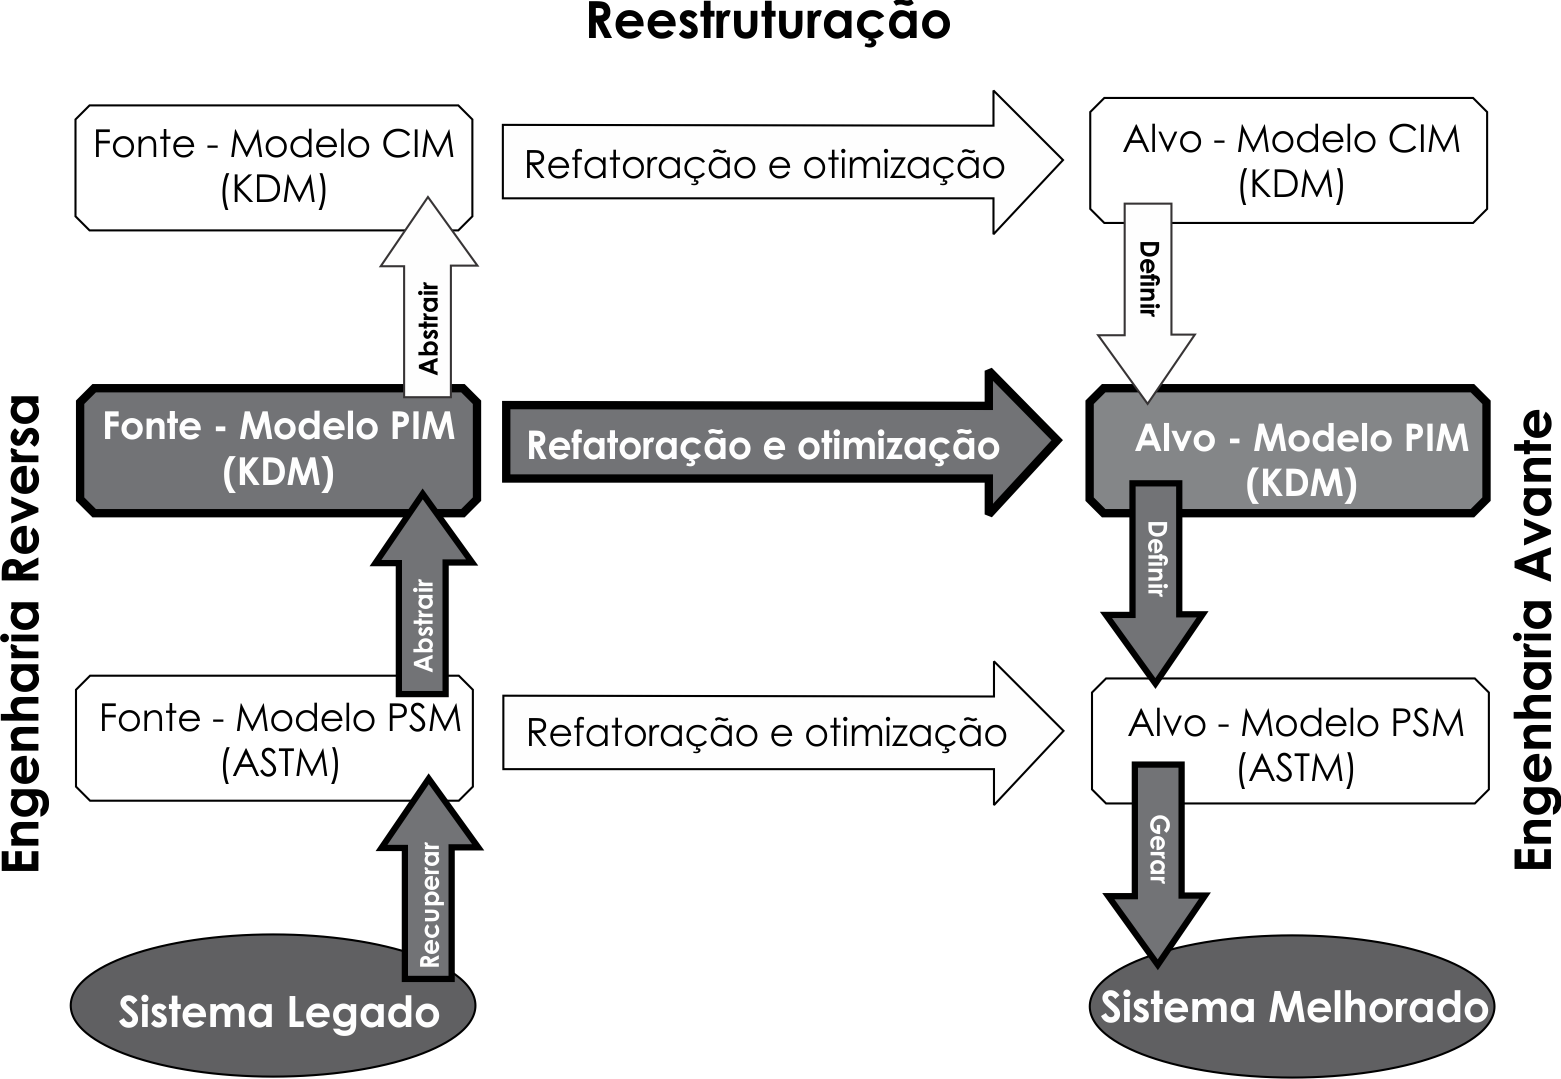
\includegraphics[scale=0.78]{images/modelo-ferradura.png}
 \fadaptada{ADM:OMG}
\end{figure}

Durante o processo da ADM todos os modelos (i.e., PSM, PIM e CIM) podem estabelecer transformações/refatorações entre si, como ilustrado na Figura~\ref{fig:horse_shoe}. Geralmente tais transformações são executadas por meio de linguagens de transformações. Como salientado no Capítulo~\ref{chapter:fundamentacao_teorica}, Seção~\ref{sec:transformacoes_de_modelos} usualmente essas transformações são implementadas utilizando diferentes linguagens de transformações que podem ser declarativas, imperativas ou híbridas. 

É importante também destacar que a ADM não tem como intuito apenas seguir todos os princípios da abordagem MDA~\cite{ADM:OMG}. Um dos principais objetivos da ADM é definir um conjunto de metamodelos, padronizados, para lidar com diferentes desafios que são encontrados hoje em dia na reengenharia de software. Dessa forma, em Novembro de 2003, a \sigla{ADMTF}{\textit{Architecture-Driven Modernization Task Force}} criou uma \sigla{RFP}{\textit{Request-for-Proposal}} que por sua vez descrevia um conjunto de metamodelos. Tais metamodelos são: (\textit{i}) Knowledge Discovery Metamodel (KDM), maiores informações sobre esse metamodelo é apresentado na seção~\ref{sec:knowledge_discovery_meta_model}, (\textit{ii}) \sigla{SMM}{\textit{Structured Metrics metamodel}} que é um metamodelo para representar e definir métricas e resultados de medições, (\textit{iii}) \sigla{ADMPR}{\textit{ADM Pattern Recognition}}, que facilita a busca de padrões em um software, (\textit{iv}) \sigla{ADMVS}{\textit{ADM Visualization Specification}}, que tem como objetivo representar visualmente metadados de uma aplicação representada em KDM, (\textit{v}) \sigla{ADMRS}{\textit{ADM Refactoring Specification}}, que almeja definir um metamodelo padronizado para especificar e definir refatorações utilizando outros metamodelos da ADM, como por exemplo o KDM. O estado atual de cada metamodelo pode ser visto na Tabela~\ref{tab:todos_os_meta_modelos_da_ADM}~\cite{ADM:OMG}. Como observado nessa tabela, alguns metamodelos ainda encontram-se em fase de desenvolvimento e outros já foram finalizadas e disponíveis pelo OMG.

% Please add the following required packages to your document preamble:
% \usepackage{multirow}
\begin{table}[h]
\centering
\caption{Estado atual dos metamodelos da ADM.}
\label{tab:todos_os_meta_modelos_da_ADM}
\begin{tabular}{|l|l|l|l|}
\hline
\multicolumn{1}{|c|}{Metamodelo}                                         & \multicolumn{1}{c|}{Situação}           & \multicolumn{1}{c|}{Versão} & \multicolumn{1}{c|}{Data}          \\ \hline
\textit{ADM Pattern Recognition} (ADMPR)                     & Em desenvolvimento &\multicolumn{1}{c|}{\textemdash}&\multicolumn{1}{c|}{\textemdash}\\ \hline
\textit{ADM Refactoring Specification} (ADMRS)               & Em desenvolvimento &\multicolumn{1}{c|}{\textemdash}&\multicolumn{1}{c|}{\textemdash}\\ \hline
\textit{ADM Visualization Specification} (ADMVS)             & Em desenvolvimento &\multicolumn{1}{c|}{\textemdash}&\multicolumn{1}{c|}{\textemdash}\\ \hline
\sigla{ASTM}{\textit{Abstract Syntax Tree Metamodel}}               & \multicolumn{1}{c|}{Disponível}         & \multicolumn{1}{c|}{1.0}    & \multicolumn{1}{c|}{2011}  \\ \hline
\textit{Knowledge Discovery Metamodel} (KDM)                 & \multicolumn{1}{c|}{Disponível}         & \multicolumn{1}{c|}{1.3}    & \multicolumn{1}{c|}{2011}   \\ \hline
\multirow{2}{*}{\textit{Structured Metrics Metamodel} (SMM)} & \multicolumn{1}{c|}{Disponível}         & \multicolumn{1}{c|}{1.0}    & \multicolumn{1}{c|}{2012}  \\ \cline{2-4} 
                                                    & Em desenvolvimento & \multicolumn{1}{c|}{1.1}    & \multicolumn{1}{c|}{2013} \\ \hline
\end{tabular}
\end{table}

É importante destacar que a abordagem proposta nesta Tese, se concentra no metamodelo KDM. Consequentemente, é de suma importância o entendimento desse metamodelo, por isso, esse metamodelo é mais detalhado neste capítulo.
KDM é um metamodelo que pode ser utilizado para representar todos os artefatos de um determinado software existente, por exemplo, o KDM contém metaclasses especificas para representar desde de código-fonte até a arquitetura de um determinado software. O KDM é um metamodelo de representação intermediária comum para sistemas existentes e seus ambientes operacionais. Utilizando esse metamodelo para sistemas existentes é possível trocar representações do sistema em modelo entre plataformas e linguagens com a finalidade de analisar, padronizar e transformar/refatorar os sistemas existentes~\cite{ADM:OMG}. 

A ideia por trás do KDM é que a comunidade comece a criar analisadores sintáticos (do inglês - \textit{parsers}) para diferentes linguagens de programação, que transforme os códigos-fontes em instâncias do metamodelo KDM. Como resultado, qualquer técnica, ferramenta e abordagem que utilize o KDM como o artefato de entrada pode ser considerado uma técnicas, ferramenta e/ou abordagem independente de linguagem e de plataforma. Por exemplo, um catálogo de refatoração para o KDM~\cite{durelli_catalogo, durelli_VEM_ferramenta} pode ser utilizado para refatorar vários sistemas independentemente da linguagem de programação. Maiores informações sobre o KDM, bem como seus pacotes, metaclasses e metarelacionamentos são apresentados a seguir.

\section{Knowledge Discovery Metamodel (KDM)}
\label{sec:knowledge_discovery_meta_model}

\sigla{KDM}{Knowledge Discovery Metamodel} é um metamodelo para representar existentes artefatos de software, seus elementos, associações, e ambientes operacionais. O KDM tem como principal objetivo permitir que engenheiros de software criem ferramentas para auxiliar a modernização de software que sejam independente de plataforma e linguagem~\cite{KDM:specification, PerezCastillo:2011jo, ADMCHAPTERR}. Além disso, o KDM facilita e assegura a interoperabilidade e troca de dados entre diferentes ferramentas. 

Um problema tradicional facilmente identificado em várias ferramentas que lidam com a reengenharia de software é que tais ferramentas analisam diversos artefatos de um determinado software (por exemplo, código-fonte, banco de dados, \textit{scripts}, etc.) para obter conhecimentos explícitos com o intuito de realizar transformações/refatorações~\cite{rosenberg, Canfora2011}. Como consequência cada ferramenta gera e analisa tais conhecimentos de forma implícita. Assim, os conhecimentos gerados são restritos a uma especifica linguagem de programação, e/ou a uma plataforma. Como resultado tais restrições podem criar dificuldades com relação a interoperabilidade entre diferentes ferramentas. O KDM fornece uma estrutura que tem com objetivo facilitar a troca de dados entre diversas ferramentas. Além disso, o KDM possui um conjunto de metaclasse e uma estrutura padronizada que fornece meios para especificar desde artefatos físicos até artefatos lógicos de um determinado sistema de software. Em virtude dessa padronização, todas as técnicas/abordagem/ferramentas que utilizam o KDM como entrada pode ser considerada independente de plataforma e linguagem, aumentando assim, a interoperabilidade e o reúso. Em 2012 o KDM tornou-se \sigla{ISO}{\emph{International Standards Organization}}~\cite{KDM:ISO} como uma estrutura que facilita a troca de dados entre as diversas ferramentas. O KDM é definido via \sigla{MOF}{\emph{Meta-Object Facility}}~\cite{MOF} e estabelece o formato de troca de dados via \sigla{XMI}{\emph{XML Metadata Interchange}}, o qual é denominado KDM XMI \emph{schema}.


Pode-se sumarizar os principais objetivos do KDM como~\cite{ADM:OMG}: (\textit{i}) KDM representa artefatos de um sistema legado como entidades, relacionamentos e atributos; (\textit{ii}) KDM suporta uma variedade de plataforma e linguagem; (\textit{iii}) KDM define uma terminologia unificada para artefatos de sistemas legados; (\textit{iv}) KDM representa estruturas lógicas e físicas de sistemas legados; (\textit{v}) KDM permite a modificação/refatoração de sistemas legados utilizando os princípios da MDA; (\textit{vi}) KDM facilita o rastreamento de mudança entre artefatos; (\textit{vii}) KDM facilita a sincronização de estruturas lógicas e físicas de um determinado sistema legado; (\textit{viii}) KDM contém metaclasses para representar desde código-fonte até metaclasses para representar elementos arquiteturais de um determinado sistema legado.

%\begin{itemize}
	%\item KDM representa artefatos de um sistema legado como entidades, relacionamentos e atributos;
	%\item KDM suporta uma  variedade de plataforma e linguagem;
%	\item KDM define uma terminologia unificada para artefatos de sistemas legados;
	%\item KDM representa estruturas lógicas e físicas de sistemas legados;
	%\item KDM permite a modificação/refatoração de sistemas legados utilizando os princípios da MDA;
	%\item KDM facilita o rastreamento de mudança entre artefatos;
	%\item KDM facilita a sincronização de estruturas lógicas e físicas de um determinado sistema legado;
	%\item KDM contém metaclasses para representar desde código-fonte até metaclasses para representar elementos arquiteturais de um determinado sistema legado.
%\end{itemize}

De acordo com~\citeonline{PerezCastillo:2011jo} o KDM possui o objetivo de cobrir um amplo escopo, para abranger um conjunto diversificado de aplicações, plataformas e linguagens de programação. Um dos principais objetivos do KDM é fornecer a capacidade de troca de metadados entre diversas ferramentas e, assim, facilitar a cooperação entre fornecedores para integrar e aumentar a interoperabilidade de diferentes abordagens, técnicas, algoritmos, etc. A fim de alcançar essa interoperabilidade e, especialmente, a integração de informações sobre diferentes facetas de um determinado sistema a partir de múltiplas ferramentas, o KDM define vários níveis de conformidade, aumentando assim a probabilidade de que duas ou mais ferramentas apoiaram o mesmo metamodelo. Além disso, o KDM também é estruturado de forma modular, seguindo o princípio da separação de interesse, com a capacidade de representar partes heterogêneas de um sistema. A separação de interesses no contexto do metamodelo KDM é alcançada por meio de pacotes, como apresentado na Figura~\ref{kdm:domain}. Cada pacote está em um nível de conformidade e possui o objetivo de definir um ponto de vista arquitetural do sistema. Em outras palavras, cada pacote do KDM constitui uma determinada ontologia para descrever e representar a grande maioria dos artefatos de sistemas de software existentes. Por exemplo, os pacotes \texttt{Code} e \texttt{Action} contêm metaclasses que representam o código-fonte de um sistema, tais como, variáveis, procedimentos/métodos/funções, chamadas para métodos, etc. Similarmente o pacote \texttt{Structure} contém metaclasses para representar elementos arquiteturais do sistema, tais como, componentes, camadas, subcomponentes, etc. O pacote \texttt{Conceptual} possui  metaclasses para definir regras de negócio do sistema.


\begin{figure}[htb]
 \caption{Pacotes e nível de conformidade do metamodelo KDM.}
 \label{kdm:domain}
 \centering
 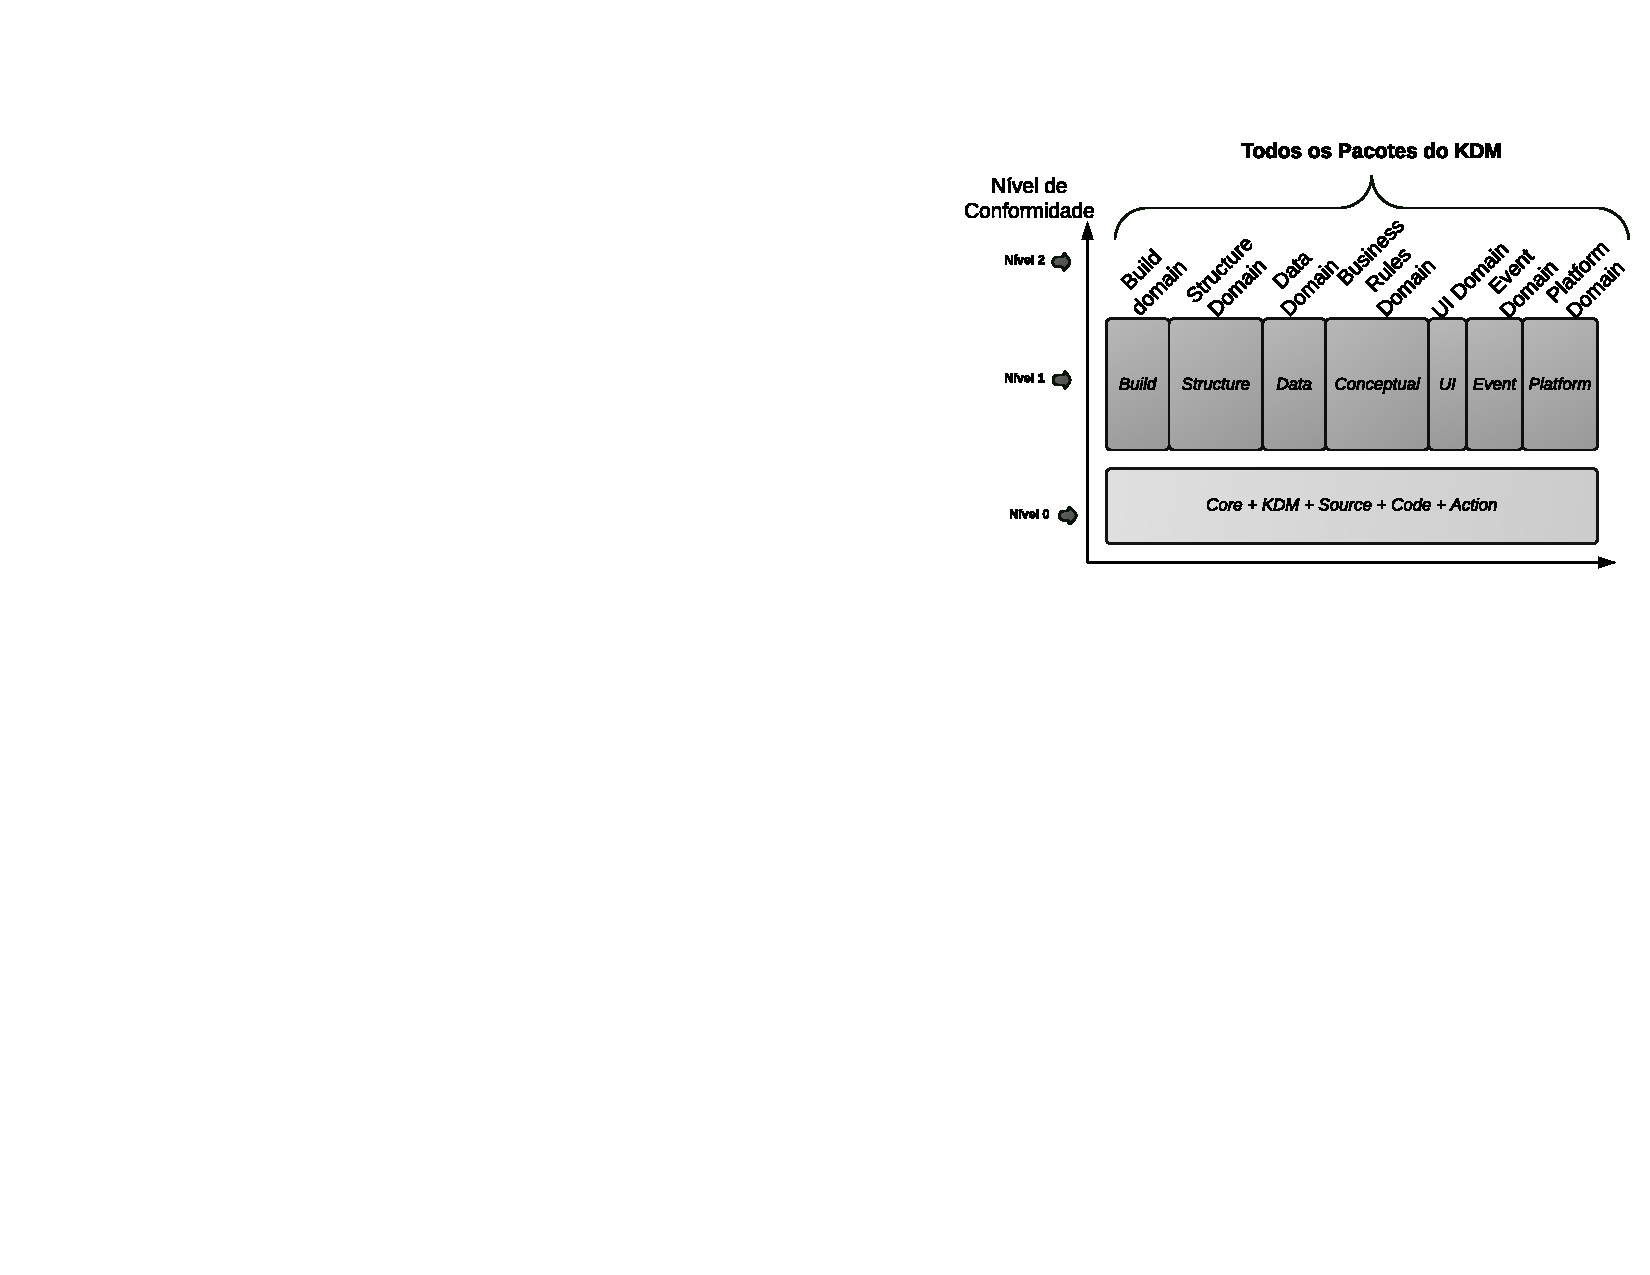
\includegraphics[scale=1]{images/kdmLevels_pacotes.pdf}
 \fadaptada{KDM:specification}
\end{figure}

Da perspectiva de um engenheiro de modernização, essa separação de interesse do KDM, por meio de pacote, significa que o engenheiro só precisa se preocupar com os pacotes do KDM que considerar necessários para as suas atividades de modernização, por exemplo, uma determinada abordagem pode necessitar apenas do pacote \texttt{Code} e \texttt{Action}, enquanto uma outra abordagem pode utilizar apenas o pacote responsável por definir elementos arquiteturais. Se essas abordagens forem evoluídas ao longo do tempo e necessitarem de outros pacotes do KDM, pacotes podem ser adicionados ao repertório da abordagem/ferramenta, conforme necessário.

Como observado na Figura~\ref{kdm:domain} o KDM possui três níveis de conformidade, nível 0, nível 1 e nível 2. Informações sobre cada nível são apresentadas a seguir:

\begin{itemize}
    \item \textbf{Nível 0}: nesse nível de conformidade são definidos os seguintes pacotes do KDM: (\textit{i})     \texttt{Core}, (\textit{ii}) \texttt{kdm}, (\textit{iii}) \texttt{Source}, (\textit{iv}) \texttt{Code} e (\textit{v}) \texttt{Action}. Esse nível de conformidade representa um denominador comum que pode servir como uma base para a interoperabilidade entre diferentes categorias de ferramentas que utilizem o metamodelo KDM. Para que uma ferramenta esteja em conformidade com o \textbf{Nível 0} ela deve fornecer completo suporte para todas as metaclasses que foram definidas nos pacotes \texttt{Core}, \texttt{kdm}, \texttt{Source}, \texttt{Code} e \texttt{Action};
    \item \textbf{Nível 1}: nesse nível os pacotes definidos no \textbf{Nível 0} são estendidos para representar outros artefatos de um determinado sistema. Esse nível define os seguintes pacotes: (\textit{i}) \texttt{Build}, (\textit{ii}) \texttt{Structure}, (\textit{iii}) \texttt{Data}, (\textit{iv}) \texttt{Conceptual}, (\textit{v}) \texttt{UI}, (\textit{vi}) \texttt{Event} e (\textit{vii}) \texttt{Platform}. Para que uma ferramenta esteja em conformidade com o \textbf{Nível 1} ela deve fornecer suporte para todos os pacotes do \textbf{Nível 0} pelo menos um do pacotes do Nível 1;
    \item \textbf{Nível 2}: esse nível é a união de todos os pacotes definidos no nível anterior. Para que uma ferramenta esteja em conformidade com o \textbf{Nível 2} ela deve fornecer suporte para todos os pacotes do \textbf{Nível 1} e pelo menos um do \textbf{Nível 2}.
\end{itemize}


Todos os pacotes do metamodelo KDM apresentado na Figura~\ref{kdm:domain} são organizados em quatro camadas de abstração. As camadas de abstração são: (\textit{i}) \sigla{CI}{Camada de Infraestrutura}: do inglês \textit{Infrastructure Layer}; (\textit{ii}) \sigla{CEP}{Camada de Elementos de Programa}: do inglês \textit{Program Elements Layer}; (\textit{iii}) \sigla{CRTE}{Camada de Recurso de Tempo de Execução}: do inglês \textit{Runtime Resource Layer}; (\textit{iv}) \sigla{CA}{Camada de Abstração}: do inglês \textit{Abstraction Layer}. Essas quatro camadas estão apresentadas esquematicamente na Figura~\ref{fig:kdm_layer}.

%\begin{itemize}
    %\item \sigla{CI}{Camada de Infraestrutura}: do inglês \textit{Infrastructure Layer};
    %\item \sigla{CEP}{Camada de Elementos de Programa}: do inglês \textit{Program Elements Layer};
    %\item \sigla{CRTE}{Camada de Recurso de Tempo de Execução}: do inglês \textit{Runtime Resource Layer};
    %\item \sigla{CA}{Camada de Abstração}: do inglês \textit{Abstraction Layer}.
%\end{itemize}


%(\textit{i}) \sigla{CI}{Camada de Infraestrutura} (do inglês \textit{Infrastructure Layer}), (\textit{ii}) \sigla{CEP}{Camada de Elementos de Programa} (do inglês \textit{Program Elements Layer}), (\textit{iii}) \sigla{CRTE}{Camada de Recurso de Tempo de Execução} (do inglês \textit{Runtime Resource Layer}) e (\textit{iv} ) \sigla{CA}{Camada de Abstração} (do inglês \textit{Abstraction Layer}). 

%Cada camada é posteriormente organizada em pacotes, como pode ser observado na Figura~\ref{fig:kdm_layer}. Por sua vez, cada pacote define um conjunto de metaclasses cujo propósito é representar o conhecimento de específicos artefatos de um determinado sistema. 

%
\begin{figure}[htb]
 \caption{Camadas e pacotes do KDM.}
 \label{fig:kdm_layer}
 \centering
 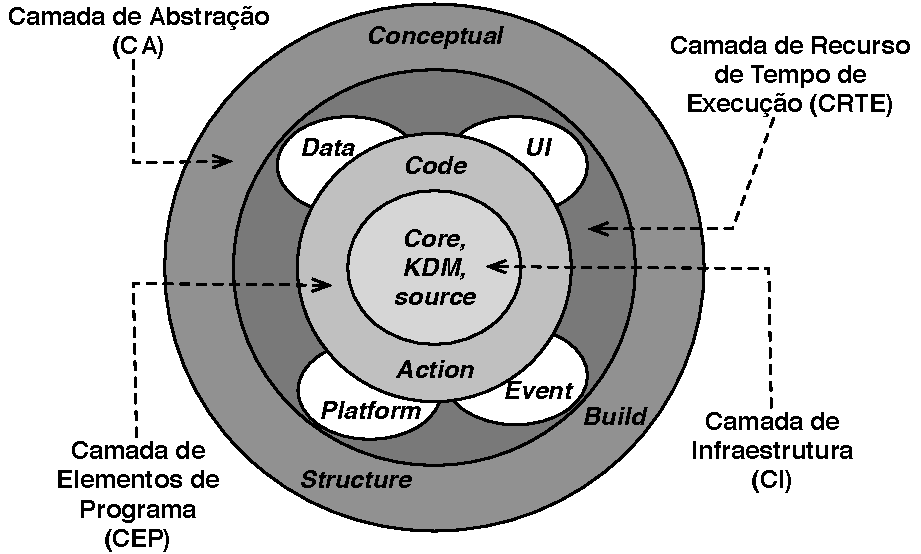
\includegraphics[scale=0.67]{images/kdm_layers.pdf}
 \fadaptada{KDM:specification}
\end{figure}
%
A camada CI contém três pacotes, são eles: (\textit{i}) \texttt{Core}, (\textit{ii}) \texttt{\aspas{kdm}} e (\textit{iii}) \texttt{Source}. Os dois primeiros pacotes, \texttt{Core} e \texttt{\aspas{kdm}}, representam a infraestrutura básica para outros pacotes do KDM e definem metaclasses e relacionamentos básicos. O pacote \texttt{Source} define o \texttt{Inventory Model}, o qual representa artefatos de software e mantém a rastreabilidade entre eles. 

A camada CEP possui dois pacotes: (\textit{i}) \texttt{Code} e (\textit{ii}) \texttt{Action}. Esses pacotes coletivamente definem o \texttt{Code Model} que contém metaclasses para representar artefatos em nível de implementação. O pacote \texttt{Code} contém um conjunto de metaclasses para representar a estrutura de um determinado programa e seus relacionamentos, enquanto que o pacote \texttt{Action} possui metaclasses para descrever o comportamento e o fluxo de dados de um programa.

A camada CRTE contém quatro pacotes: (\textit{i}) \texttt{Data}, (\textit{ii}) \texttt{Platform}, (\textit{iii}) \texttt{Event} e (\textit{iv}) \texttt{UI}. Coletivamente tais pacotes representam a estrutura e comportamento de recursos de tempo de execução do sistema. Tais pacotes são diretamente instanciados por meio da definição de recursos, abstração do \texttt{Code Model}, ou são manualmente instanciado pelo engenheiro de modernização. A rastreabilidade entre os elementos abstraídos e os elementos físicos (por exemplo, código-fonte) é mantida pelo meta-atributo denominado \texttt{implementation}. Finalmente, a camada CA contém três pacotes: (\textit{i}) \texttt{Conceptual}, (\textit{ii}) \texttt{Structure} e (\textit{iii}) \texttt{Build}. Esses pacotes possuem metaclasses para representar o maior nível de abstração de um sistema, por exemplo, a estrutura do sistema, regras de negócios, documentações do sistema, etc.

Uma característica importante de ser observada e ressaltada é que todas as camadas do KDM interagem, significando que todas as camadas são conectadas de alguma forma\footnote{Essa conectividade entre os elementos de cada camada são mantidos por um conjunto de meta-atributo, por exemplo, o meta-atributo \texttt{implementation}.}, como consequência se uma mudança/refatoração é realizada em uma camada especifica, a mudança/refatoração deve ser propagada para outras camadas com o intuito de manter todas as camadas sincronizadas e consistentes preservando assim a estrutura estática do KDM e o comportamento do código representado em KDM. Nas próximas seções são apresentados os principais pacotes do metamodelo KDM que compõem o contexto para o desenvolvimento deste trabalho.

\subsection{Pacote Code}\label{subsection:codePackage}

O pacote $\mathtt{Code}$ define um conjunto de metaclasses cujo propósito é representar unidades de programa em nível de implementação e as suas associações. O pacote também inclui metaclasses que representam elementos de programa comuns suportados por várias linguagens de programação, como tipo de dados, classes, procedimentos, macros, protótipos e \textit{templates}.


Em uma determinada instância do KDM, cada elemento do pacote~$\mathtt{code}$ representa alguma construção em uma linguagem de programação, determinada pela linguagem de programação utilizada no sistema. Na Figura~\ref{fig:CodeModel} um trecho do~$\mathtt{CodeModel}$\footnote{O diagrama de classes do $\mathtt{CodeModel}$ mostrado aqui só representa o conjunto de metaclasses e os seus respectivos relacionamentos lógicos, para informações completas, verifique a especificação do KDM~\cite{KDM:specification}.} é retratado.

%In a given KDM instance, each instance of the code metamodel element represents some programming language construct, determined by the programming language of the existing software system. Each instance of a code metamodel element corresponds to a certain region of the source code in one of the artifacts of the existing software system. Figure~\ref{fig:CodeModel} the \texttt{CodeModel}\footnote{The \texttt{CodeModel} class diagram presented herein shows just a set of the metaclasses and their logical relationship, for complete information please see the KDM specification} is depicted, it represents parts of the KDM infrastructure. 

\begin{figure}[!ht]
	\centering
	% Requires \usepackage{graphicx}
	\caption{Diagrama de classes - $\mathtt{CodeModel}$}
	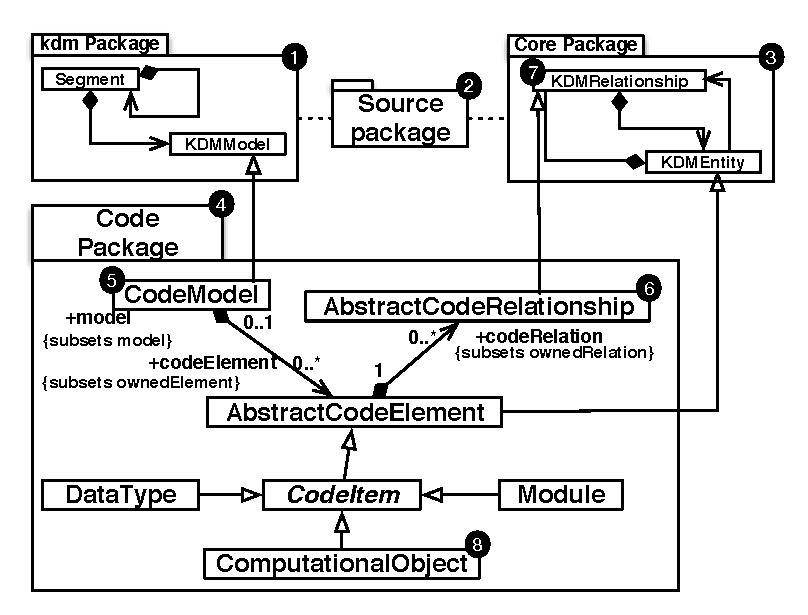
\includegraphics[scale=0.67]{images/codeModel}
	\label{fig:CodeModel}
	\fadaptada{KDM:specification}
\end{figure}

A metaclasse \texttt{CodeModel} representa um contêiner para outras instâncias de elementos do tipo~$\mathtt{Code}$. O pacote $\mathtt{Code}$ \ding{205} depende dos outros pacotes $\mathtt{kdm}$ \ding{202}, $\mathtt{Source}$ \ding{203} e $\mathtt{Core}$ \ding{204}. A metaclasse $\mathtt{CodeModel}$ \ding{206} é um modelo que possui coleções de fatos sobre o sistema de software, correspondentes ao domínio $\mathtt{Code}$. Ela possui uma associação  $\mathtt{codeElement:AbstractCodeElement[0..*]}$ permitindo a adição de novos elementos de código, por exemplo, métodos, atributos, etc. A metaclasse  $\mathtt{AbstractCodeRelationship}$ \ding{207} representa qualquer relacionamento determinado por em uma linguagem de programação. Por sua vez, a metaclasse $\mathtt{ComputationalObject}$ representa os elementos determinados pela linguagem de programação, que descreve certos objetos computacionais em tempo de execução, por exemplo, métodos e variáveis.

%This metamodel element is a container for other \texttt{code} element instances. As can be observed in Figure~\ref{fig:CodeModel} the \texttt{Code} package \ding{205} depends on the \texttt{kdm} \ding{202}, \texttt{Source} \ding{203}, and \texttt{Core} \ding{204} packages. The meta-class \texttt{CodeModel} \ding{206} is the specific KDM model that owns collections of facts about the existing software system such that these facts correspond to the \texttt{Code} domain, its superclass is \texttt{KDMModel}. It has as association \texttt{codeElement:AbstractCodeElement[0..*]} meaning that one shall arrange code elements (e.g., methods, fields, etc) into one or more code models. The \texttt{AbstractCodeRelationship} \ding{207} is an abstract meta-class representing any relationship determined by a programming language, it is also used to constrain the subclasses of \texttt{KDMRelationship} (see Figure~\ref{fig:CodeModel} \ding{208}) in the \texttt{Code} model. The meta-class \texttt{ComputationalObject} represents the named elements determined by the programming language, which describe certain computational objects at the runtime, for example, methods, and variables.

O pacote~$\mathtt{Code}$ consiste em um total de 24 metaclasses; tais metaclasses são um arranjo de abstrações para representar toda, ou a grande maioria, da estrutura estática de um terminado código-fonte dado um linguagem de programação, seja ela procedural ou orientada a objetos~\cite{KDM:specification}. Na Tabela~\ref{tab:meta_classes_pacoteCODE} algumas metaclasses são apresentadas. Como pode ser observado algumas metaclasses podem ser diretamente elucidadas e mapeadas, como por exemplo, \aspas{classes} e \aspas{interfaces} construções facilmente encontradas em linguagens orientadas a objetos podem ser facilmente mapeada para as metaclasses denominada $\mathtt{ClassUnit}$ e $\mathtt{InterfaceUnit}$, respectivamente. Um mapeamento mais completo entre elementos estruturais e metaclasses do KDM pode ser identificado em~\citeonline{bruno_marinho_dissertacao} e no Capítulo~\ref{chapter:catalogo_refactoring_KDM}. Uma representação dessas metaclasses, bem como seus relacionamentos são apresentados em diagrama de classe na Figura~\ref{fig:classUnit_e_InterfaceUnit}.

\begin{figure}[!ht]
	\centering
	\caption{Diagrama de classes elucidando as metaclasses \texttt{ClassUnit} e \texttt{InterfaceUnit}}
	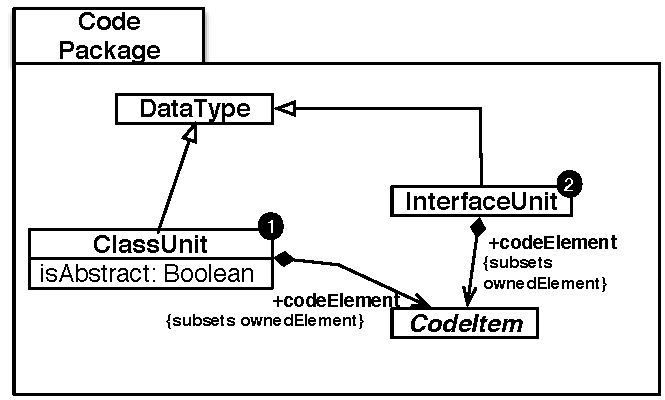
\includegraphics[scale=0.67]{images/ClassUnit_InterfaceUnit}
	\label{fig:classUnit_e_InterfaceUnit}
	\fadaptada{KDM:specification}
\end{figure}

%The whole \texttt{Code} package consists of $24$ metaclasses\footnote{Note that not all the meta-class are shown in Figure~\ref{fig:CodeModel}} and contains all the abstract elements for modeling the static structure of the source code. In Table~\ref{tab:mappingCodeToKDM} is depicted some of them. This table identifies KDM metaclasses possessing similar characteristics to the static structure of the source code. Some metaclasses can be direct mapped, such as class from object-oriented language, which can be easily mapped to the \texttt{ClassUnit} meta-class from KDM. For instance, the meta-class \texttt{Package} is a subtype for \texttt{Module} that logical collections of program elements, as directly supported by some programming languages, such as Java. 

\begin{table}[h]
\centering
\caption{Metaclasses para modelagem de estruturas estáticas do código-fonte.}
\label{tab:meta_classes_pacoteCODE}
\begin{tabular}{|l|l|}
\hline
Elemento do Código-Fonte & metaclasses do KDM \\ \hline
\multicolumn{1}{|c|}{Classe}                   & \multicolumn{1}{|c|}{\texttt{ClassUnit}}           \\ \hline
\multicolumn{1}{|c|}{Interface}                & \multicolumn{1}{|c|}{\texttt{InterfaceUnit}}       \\ \hline
\multicolumn{1}{|c|}{Método}                   & \multicolumn{1}{|c|}{\texttt{MethodUnit}}          \\ \hline
\multicolumn{1}{|c|}{Atributo}                 & \multicolumn{1}{|c|}{\texttt{StorableUnit}}        \\ \hline
\multicolumn{1}{|c|}{Variável Local}           & \multicolumn{1}{|c|}{\texttt{MemberUnit}}          \\ \hline
\multicolumn{1}{|c|}{Parâmetro}                & \multicolumn{1}{|c|}{\texttt{ParameterUnit}}       \\ \hline
\multicolumn{1}{|c|}{Associação}               & \multicolumn{1}{|c|}{\texttt{KDMRelationShip}}     \\ \hline
\end{tabular}
\end{table}

%\begin{table}[!h]
	%\caption{metaclasses para modelagem de estruturas estáticas do código fonte}
%	\label{tab:mappingCodeToKDM}
%	\centering
%	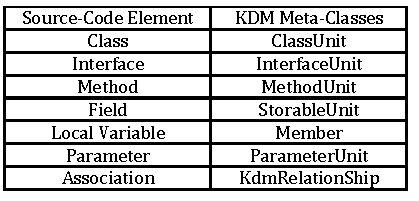
\includegraphics[scale=1]{images/tabela_comparativo_KDM_code_com_source_code}
%\end{table}

$\mathtt{ClassUnit}$ e $\mathtt{InterfaceUnit}$ representam \aspas{classes} e \aspas{interfaces} que são definidas por usuários de linguagens orientadas a objeto. Ambas metaclasses possuem caracteristicas e relacionamentos similares, como observado na Figura~\ref{fig:classUnit_e_InterfaceUnit} \ding{202} e \ding{203}. Uma das diferenças que pode ser destacada é que a metaclasse ~$\mathtt{ClassUnit}$ contém um meta-atributo~$\mathtt{isAbstract:Boolean}$, o qual é utilizado para especificar se uma classe é ou não abstrata. $\mathtt{ClassUnit}$ e $\mathtt{InterfaceUnit}$ podem conter um coleção de elementos que seja do tipo ~$\mathtt{CodeItem}$, por exemplo,~$\mathtt{StorableUnit}$ ou ~$\mathtt{MethodUnit}$. Além disso, tais metaclasses  possuem uma meta-associação denominada ~$\mathtt{codeElement:CodeItem[0..*]}$ que é utilizada para agrupar todos os membros da classe, por exemplo, construtores, métodos, atributos, etc. Na Figura~\ref{fig:StorableUnit_MethodUnit} é apresentado os meta-atributos e metarelacionamentos das metaclasses \texttt{StorableUnit} \ding{204}, \texttt{MethodUnit} \ding{205}, \texttt{ParameterUnit} \ding{207} e \texttt{MemberUnit} \ding{206}.

\begin{figure}[!ht]
	\centering
	% Requires \usepackage{graphicx}
	\caption{Diagrama de classes elucidando as metaclasses \texttt{StorableUnit}, \texttt{MethodUnit}, \texttt{ParameterUnit} e \texttt{MemberUnit}}
	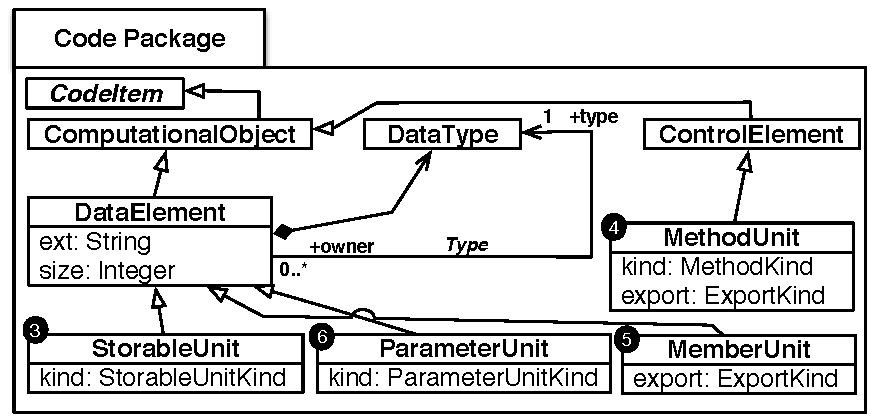
\includegraphics[scale=0.67]{images/StorableUnit_MethodUnit2}
	\label{fig:StorableUnit_MethodUnit}
	\fadaptada{KDM:specification}
\end{figure}


%As stated before, the meta-class \texttt{ClassUnit} represents user-defined classes in object-oriented languages. A class datatype is a named datatype that represents a class: an ordered collection of named elements, each of which can be another \texttt{CodeItem}, such as a \texttt{StorableUnit} or a \texttt{MethodUnit}. The meta-class \texttt{ClassUnit} contains a meta-attribute \texttt{isAbstract:Boolean} used to specify if the class is abstract or not. \texttt{ClassUnit} also has an meta-association named \texttt{codeElement:CodeItem[0..*]} that is used to group all class's members, e.g., fields, constructor, methods, etc. 

%Similarmente, a metaclasse~$\mathtt{InterfaceUnit}$ representa o conceito comum a várias linguagens de programação. Ela é uma subclasse de~$\mathtt{DataType}$, assim como~$\mathtt{ClassUnit}$.~$\mathtt{InterfaceUnit}$ também possui uma meta associação chamada~$\mathtt{codeElement:CodeItem[0..*]}$ que representa tipos de dados tal como~$\mathtt{MethodUnit}$.

%Similarly, the meta-class \texttt{InterfaceUnit} represents the interface concept common to various programming languages. It is also a subclass of \texttt{Datatype} as \texttt{ClassUnit}. \texttt{InterfaceUnit} also has an meta-association named \texttt{codeElement:CodeItem[0..*]} that represent data types as well as \texttt{MethodUnits}.

$\mathtt{StorableUnit}$ representa um atributo em um sistema de software - um objeto computacional para que diferentes valores do mesmo tipo de dados possa ser associado em vezes diferentes. Ele é usado para representar as variáveis globais e locais. Ele contém uma meta atributo~$\mathtt{String}$ usado para definir o nome das variáveis.~$\mathtt{StorableUnit}$ também tem a associação~$\mathtt{type:DataType[1]}$, a qual é herdada da metaclasse~$\mathtt{DataElement}$, e é utilizado para especificar o tipo da variável (\textit{int, char, boolean, numeric}, etc). Ele também tem uma enumeração ~$\mathtt{kind:StorableUnit}$, que descreve várias propriedades comuns de um ~$\mathtt{StorableUnit}$ relacionado com o seu ciclo de vida, por exemplo, sua visibilidade (\textit{private, public, protected}, etc).

%\texttt{StorableUnit} represents a variable of existing software system - a computational object to which different values of the same datatype can be associated at different times. It is used to represent both global and local variables. It contains a meta-attribute \texttt{name:String} used to set the name of the variables. \texttt{StorableUnit} also has the association \texttt{type:Datatype[1]} used to specify the variable's type. It also has a enumeration \texttt{kind:StorableKind}, it describes several common properties of a \texttt{StorableUnit} related to their life-cycle, visibility, and memory type. 

~$\mathtt{MethodUnit}$ como o próprio nome sugere representa métodos que são identificados em ~$\mathtt{ClassUnit}$ ou~$\mathtt{InterfaceUnit}$. Ele também é usado para representar construtores e destrutores. Possui como meta-atributos~$\mathtt{name:String}$,~$\mathtt{kind:MethodKind}$ e ~$\mathtt{export:ExportKind}$. O primeiro é usado para descrever o nome de um método. O segundo meta-atributo é uma enumeração que define especificações adicionais do tipo de método, ou seja, é possível especificar se a instância do método é um construtor, destrutor, ou um método normal. O último representa a visibilidade do método (\textit{private, public, protected}, etc).

%\texttt{MethodUnit} represents member functions owned by either \texttt{ClassUnit} or \texttt{InterfaceUnit}. It is also used to represent user-defined operators, constructors, and destructors. It owns as meta-attributes \texttt{name:String}, \texttt{kind:MethodKind}, and \texttt{export: ExportKind}. The fist one is used to describe to name of a method. The second meta-attribute is an enumeration that defines additional specification of the kind of method, i.e., it is possible to specify if the method's instance is a constructor, destructor, abstract, etc. The last one represents the visibility of the method, i.e., \texttt{public}, \texttt{private}, \texttt{protected}.

A fim de entender como o KDM é utilizado para representar estruturas um determinado programa, no Código-fonte~\ref{lst:example_kdm_instance} é mostrado um exemplo simplificado escrito em Java. O correspondente KDM, embora simplificado, é apresentado na Figura~\ref{fig:kdm_instance_Java}. Por questões de simplicidade e para facilitar o entendimento, essa figura ilustra a instância do KDM em forma de um diagrama de objetos; é possível notar que este diagrama representa o código-fonte como uma árvore, na qual cada nó representa uma metaclasses do KDM. Como pode ser visto na Figura~\ref{fig:kdm_instance_Java}, a metaclasse raiz é ~$\mathtt{Segment}$, que é um recipiente para um conjunto significativo de fatos sobre um sistema de software existente. Cada~$\mathtt{Segment}$ pode incluir uma ou mais instâncias de modelos do KDM, como~$\mathtt{CodeModel}$ e~$\mathtt{StructureModel}$.

%In order to fully understand how KDM is used to represent the source code of a specific program, in Listing~\ref{lst:example_kdm_instance} is shown a simplified example in Java. The corresponding, though simplified KDM instance is depicted in Figure~\ref{fig:kdm_instance_Java}. It illustrates a KDM instance as a UML object diagram for the sake of simplicity, note that this diagram represents the source code as a tree of nodes containing some KDM's metaclasses. As can be seen in Figure~\ref{fig:kdm_instance_Java} the root meta-class is \texttt{Segment}, which is a container for a meaningful set of facts about an existing software system. Each \texttt{Segment} may include one or more KDM model instances, such as \texttt{CodeModel} and \texttt{StructureModel}. As stated earlier, the \texttt{CodeModel} is the specific KDM container for other \texttt{code} element instances (see Figure~\ref{fig:CodeModel}). 

Analisando tanto o Código-fonte~\ref{lst:example_kdm_instance} quanto a Figura~\ref{fig:kdm_instance_Java} é evidente que cada estrutura estática do código-fonte tem uma metaclasse específica em KDM para representá-la. Por exemplo, a declaração \textit{package} \textit{model} na Linha 1 do Código-fonte~\ref{lst:example_kdm_instance} \ding{202} é representada em KDM pela metaclasse ~$\mathtt{package}$, como visto na Figura~\ref{fig:kdm_instance_Java} \ding{202}. Posteriormente, como apresentado no Código-fonte~\ref{lst:example_kdm_instance} \ding {203} uma classe~$\mathtt{Car}$ é declarada. Essa classe herda caracteristicas da classe~$\mathtt{Vehicle}$, no Java isso é feito por meio da palavra-chave~$\mathtt{extends}$ seguido do nome de uma classe, conforme por ser observado no Código-fonte~\ref{lst:example_kdm_instance} \ding{204} e \ding{205}. A metaclasse~$\mathtt{Extends}$ representa o conceito de herança em KDM. Como mostrado na Figura~\ref{fig:kdm_instance_Java} \ding {204} a metaclasse~$\mathtt{Extends}$ possui duas associações,~$\mathtt{to}$ e~$\mathtt{from}$, o primeiro representa a classe pai (\textit{super class}), e o último a classe filha(\textit{sub-class}). Neste contexto, a classe~$\mathtt{Car}$ e classe pai de~$\mathtt{Vehicle}$, como mostrado na Figura~\ref{fig:kdm_instance_Java} \ding{205}. Finalmente, o atributo~$\mathtt{name}$ e o método~$\mathtt{getName()}$ (ver Código-fonte~\ref{lst:example_kdm_instance} \ding {206} e \ding {207}, respectivamente) são mapeados para os correspondentes elementos do KDM,~$\mathtt{StorableUnit}$ e~$\mathtt{MethodUnit}$ (ver Figura ~\ref{fig:kdm_instance_Java} \ding {206} e \ding {207}). 

%Analyzing both the Listing~\ref{lst:example_kdm_instance} and the Figure~\ref{fig:kdm_instance_Java} it is evident that each static structure of the source code has a meta-class in KDM to represent it. For instance, the package model in Line 1 of Listing~\ref{lst:example_kdm_instance} \ding{202} is represented in KDM by the meta-class named \texttt{Package}, see Figure~\ref{fig:kdm_instance_Java} \ding{202}. In addition, the class \texttt{Car} is declared, see Listing~\ref{lst:example_kdm_instance} \ding{203}. It also inherit from class \texttt{Vehicle}, in the Java this is accomplished by using the keyword \texttt{extends} following of a class, see Listing~\ref{lst:example_kdm_instance}  \ding{204} and \ding{205}. The meta-class \texttt{Extends} represents inheritance in KDM models. As shown in Figure~\ref{fig:kdm_instance_Java} \ding{204} the meta-class \texttt{Extends} has two association, \texttt{to} and \texttt{from}, the former represents the parent class (super class), and the latter represents the child class (sub-class). In this context, the child is the class \texttt{Car} and the parent class is \texttt{Vehicle}, which is depicted in Figure~\ref{fig:kdm_instance_Java} \ding{205}. Finally, the variable \texttt{name}, and the method \texttt{getName()} (see Listing~\ref{lst:example_kdm_instance} \ding{206}, and \ding{207}) are mapped to corresponding instances of the KDM elements, \texttt{StorableUnit}, and \texttt{MethodUnit} (see Figure~\ref{fig:kdm_instance_Java} \ding{206}, and \ding{207}). 


\noindent\begin{minipage}{.53\textwidth}
	\begin{codigo}[caption={[Parte de código Java para ilustrar como o KDM é usado para representar o código fonte.] Simples código em java.},escapeinside={(*@}{@*)}, basicstyle=\footnotesize, label={lst:example_kdm_instance}]{Name}
	(*@\ding{202}@*) package model;
	(*@\ding{203}@*) public class Car (*@\ding{204}@*) extends  
	(*@\ding{205}@*) Vehicle{
	(*@\ding{229}@*)(*@\ding{206}@*) private String name;
	(*@\ding{229}@*)(*@\ding{207}@*) public String getName(){
	(*@\ldots @*)
	}
	}
	\end{codigo}
\end{minipage}\hfill
\begin{minipage}{.45\textwidth}
	\centering
	% Requires \usepackage{graphicx}
	\captionof{figure}{Instância KDM correspondente ao Código-fonte~\ref{lst:example_kdm_instance}}
	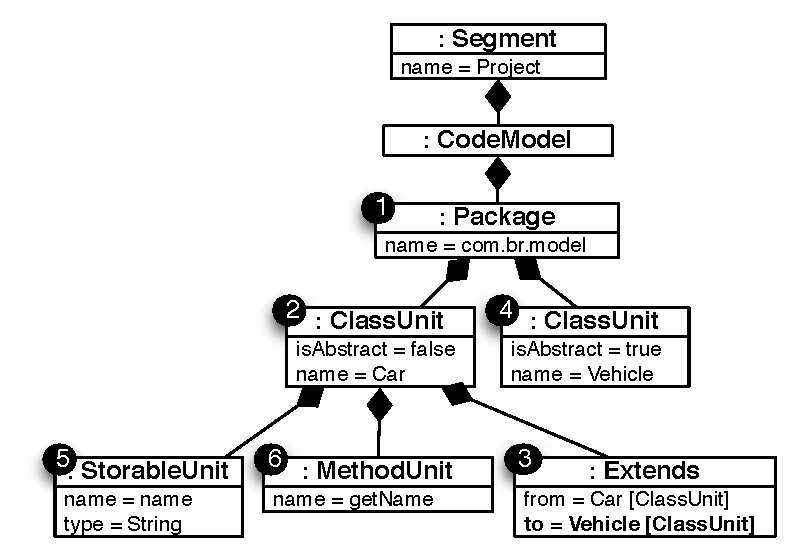
\includegraphics[scale=0.6]{images/kdm_instance_java_correspoding_2_with_extends}
	\fautor
	\label{fig:kdm_instance_Java}
\end{minipage}


Apenas metaclasses utilizadas para representar estruturas e construções estáticas foram apresentadas. No entanto, o KDM contém um pacote que permite a representação de construções dinâmicas, em outras palavras, o pacote \textit{Action} contém metaclasses cuja finalidade é permitir e representar comportamento em nível de execução. Na seção a seguir mais informações sobre esse pacote é apresentado.

\subsection{Pacote Action}\label{sec:actionPackage}

O pacote~$\mathtt{Action}$ define um conjunto de metaclasses, cujo propósito é o de representar descrições de comportamento em nível de implementação estabelecido por linguagens de programação, por exemplo, declarações, operadores, condições e as suas associações. A Figura ~\ref{fig:actionModel} \ding {202} mostra o pacote~$\mathtt{Action}$ e algumas de suas metaclasses. Como pode ser observado, este pacote estende o pacote~$\mathtt{Code}$ (ver a Figura~\ref {fig:actionModel} \ding {208}).

%The \texttt{Action} package defines a set of metaclasses whose purpose is to represent implementation-level behavior descriptions determined by programming languages, for example statements, operators, conditions, features, as well as their associations, for example control and data flow. The Figure~\ref{fig:actionModel} \ding{202} shows the\texttt{Action} package and some of its metaclasses. As can be observed it extends the KDM \texttt{Code} package (see Figure~\ref{fig:actionModel} \ding{208}). 

\begin{figure}[!ht]
	\centering
	% Requires \usepackage{graphicx}
	\caption{Diagrama de classes ilustrando o pacote~$\mathtt{Action}$.}
	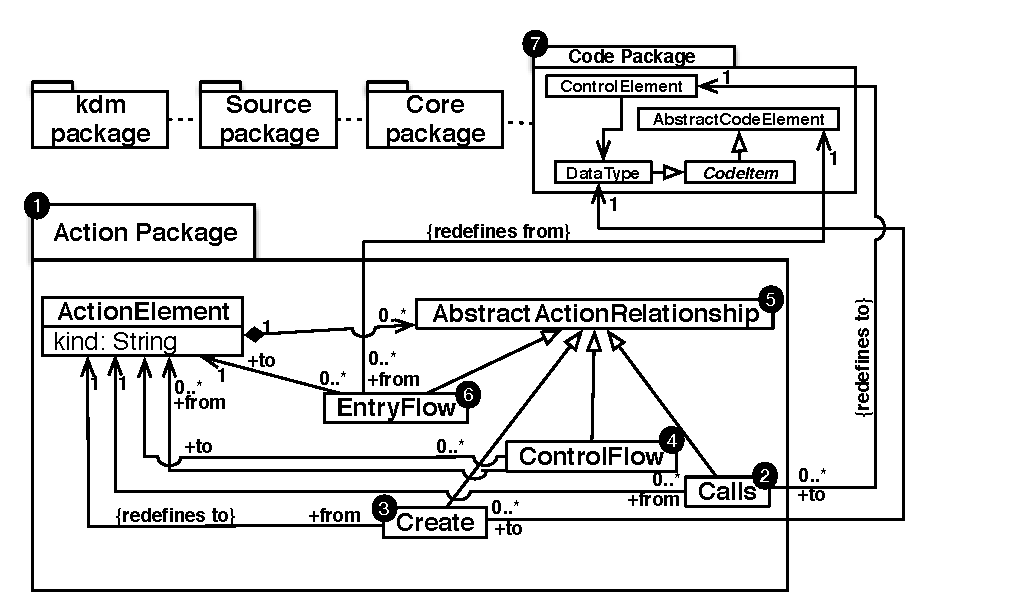
\includegraphics[scale=0.67]{images/ActionModel_Class_Diagram}
	\label{fig:actionModel}
	\fadaptada{KDM:specification}
\end{figure}

O pacote~$\mathtt{Action}$ é composto por 11 diagramas de classe, ele também depende dos pacotes~$\mathtt{Core}$, ~$\mathtt{kdm}$ e ~$\mathtt{Source}$, e  principalmente do pacote~$\mathtt{Code}$. No entanto, o pacote~$\mathtt{Action}$ segue o padrão uniforme para os modelos KDM e estende o KDM com metaclasses específicas relacionadas com o comportamento do nível de implementação. O pacote~$\mathtt{Action}$ se desvia de um padrão uniforme para os modelos KDM porque ele não define um modelo KDM separado, mas estende o pacote~$\mathtt{Code}$.  Por isso, cada metaclasse do pacote ~$\mathtt{Action}$ é uma subclasse de~$\mathtt{AbstractCodeElement}$, conforme destacado na Figura~\ref{fig:actionModel}. O pacote~$\mathtt{Action}$ define a maioria das metaclasses que tem como objetivo representar comportamentos para as construções estáticas definidas no pacote~$\mathtt{Code}$. Assim, ambos pacotes constituem a CEP, como mostrado na Figura~\ref{fig:kdm_layer}.

%The \texttt{Action} package consists of 11 class diagrams, it also depends on the \texttt{Core}, \texttt{kdm}, \texttt{Source}, and mainly \texttt{Code}. However, the \texttt{Action} package follows the uniform pattern for KDM models and extends the KDM with specific metaclasses related to implementation-level behavior. The \texttt{Action} package deviates from a uniform pattern for KDM models because it does not define a separate KDM model, but rather extends the \texttt{Code}, which is presented in Section~\ref{codePackage}. Therefore each \texttt{Action} metaclasses is a subclass of \texttt{AbstractCodeElement}, as highlighted in Figure~\ref{fig:actionModel}. \texttt{Action} package defines most of the relationship types to the \texttt{Code} model. Together, \texttt{Action}, and \texttt{Code} packages constitute the Program Elements Layer of KDM as depicted in Figure~\ref{fig:all_kdm_layers}. 

A metaclasse~$\mathtt{AbstractionActionRelationship}$ apresentada na Figura~\ref{fig:actionModel} \ding{206} é a metaclasse pai usada para representar várias relações que se originam a partir de um~$\mathtt{ActionElement}$. Além disso, essa metaclasse~$\mathtt{AbstractionActionRelationship}$ possui metaclasses específicas; algumas delas estão representadas na Figura~\ref{fig:actionModel}, por exemplo, as metaclasses~$\mathtt{Calls}$ \ding {203},~$\mathtt{Creates}$ \ding {204},~$\mathtt{ControlFlow}$ \ding {205} e~$\mathtt{EntryFlow}$ \ding{207}.

%The meta-class \texttt{AbstractActionRelationship} presented in Figure~\ref{fig:actionModel} \ding{206} is the parent class used to represent various KDM relationships that originate from an \texttt{ActionElement}. The meta-class \texttt{AbstractActionRelationship} owns specific metaclasses. Some of them are depicted in Figure~\ref{fig:actionModel}, for example, the metaclasses \texttt{Calls} \ding{203}, \texttt{Create} \ding{204}, \texttt{ControlFlow} \ding{205}, and \texttt{EntryFlow} \ding{207}.

O relacionamento~$\mathtt{Calls}$ corresponde a uma chamada para um procedimento, um método estático, um método não-estático de uma instância particular de um objeto, um método virtual, ou um elemento de interface.~$\mathtt{Calls}$ possui duas associações, são elas: ~$\mathtt{ActionElement[1]}$ e ~$\mathtt{ControlElement[1]}$. O primeiro representa o elemento de ação a partir do qual a relação chamada origina, a segunda associação representa o elemento alvo.

%\texttt{Calls} relationship corresponds to ``invoke'' operation on a procedure type. It can represent a call to a procedure, a static method, a non-static method of a particular object instance, a virtual method, or an interface element. \texttt{Calls} has two associations, they are: \texttt{from:ActionElement[1]} and \texttt{to:ControlElement[1]}. The first one represents the action element from which the call relation originates. The second association represents the target \texttt{ControlElement}.

A metaclasse~$\mathtt{Creates}$ representa uma associação entre um elemento de ação que \aspas{cria} uma nova instância de um determinado elemento de dados. Por exemplo, em Java essa metaclasse corresponde a palavra-chave \textit{new} utilizada para instânciar um novo objeto. $\mathtt{Creates}$ também possui duas associações:~$\mathtt{ActionElement[1]}$ e~$\mathtt{DataType[1]}$. Similar a metaclasse~$\mathtt{Calls}$, a primeira associação representa o elemento que possui o relacionamento e a segunda representa o elemento de dados (objeto) que é instanciado pelo~$\mathtt{ActionElement}$.

%The meta-class \texttt{Create} represents an association between an action element that ``creates'' a new instance of a certain data element to the corresponding datatype according to the semantics of the programming language of the existing software system. It also has association, \texttt{from:ActionElement[1]} and \texttt{to:Datatype[1]}. Similarly, to the meta-class \texttt{Calls}, the first association represents the element that owns the \texttt{Creates} relationship. The second one illustrates the \texttt{DataElement} that is instantiated by the \texttt{ActionElement}. 

O~$\mathtt{ControlFlow}$ é um elemento de modelagem genérica que representa relação de fluxo de controle entre dois~$\mathtt{ActionElements}$. Além disso, é uma submetaclasse com elementos de modelagem mais específicas. O~$\mathtt{EntryFlow}$ é um elemento de modelagem que representa um fluxo inicial de controle em um elemento KDM. O relacionamento~$\mathtt{EntryFlow}$ é usado de uma maneira uniforme para descrever os pontos de entrada para outros elementos de código KDM.

%The \texttt{ControlFlow} is a generic modeling element that represents control flow relation between two \texttt{ActionElements}. It is further subclassed with more specific modeling elements. The \texttt{EntryFlow} is a modeling element that represents an initial flow of control into a KDM element. The \texttt{EntryFlow} relationship is used in a uniform way for describing entry points to other KDM code elements. 

A fim de compreender como o pacote~$\mathtt{Action}$ é usado no KDM, no Código-fonte~\ref{lst:example_kdm_instance_2} é mostrado um simples método implementado em Java. Neste método é criada uma instância de~$\mathtt{Car}$ e seu método de acesso é invocado. Uma possível correspondente instância do KDM simplificada é apresentada na Figura~\ref{fig:kdm_instance_Java_action}. Nota-se que, o diamante em destaque na cor cinza e anexado com três pontos (\ldots) ilustra que outras metaclasses não são mostrados com o intuito de simplificar a figura.

%In order to comprehend  how the \texttt{Action} package is used in KDM, in Listing~\ref{lst:example_kdm_instance_2} shows a simple method implemented in Java. In this method is created an instance of \texttt{Car} and an accessor method of it is called, ie., the \texttt{getName()}. The corresponding simplified KDM instance is depicted in Figure~\ref{fig:kdm_instance_Java_action}. Please note that, the diamond highlighted in grey and attached with three dots (\ldots) illustrates that other metaclasses are not shown in order to simplify the figure.  

\noindent\begin{minipage}{.43\textwidth}
	\begin{codigo}[caption={[Pedaço de código Java para ilustrar como o pacote~$\mathtt{Action}$ funciona.] Método \texttt{e1} ilustrando como o Pacote \texttt{Action} funciona.}, escapeinside={(*@}{@*)}, basicstyle=\footnotesize, label={lst:example_kdm_instance_2}]{Name}
	(*@\ldots @*)
	public void e1 (*@\ding{202}@*)(){
	Car myCar (*@\ding{203}@*) = new Car() (*@\ding{204}@*);
	(*@\ding{229}@*)myCar.getName() (*@\ding{205}@*);
	}
	(*@\ldots @*)
	\end{codigo}
\end{minipage}\hfill
\begin{minipage}{.65\textwidth}
	\centering
	\captionof{figure}{Instância KDM correspondente ao Código-fonte~\ref{lst:example_kdm_instance_2}}
	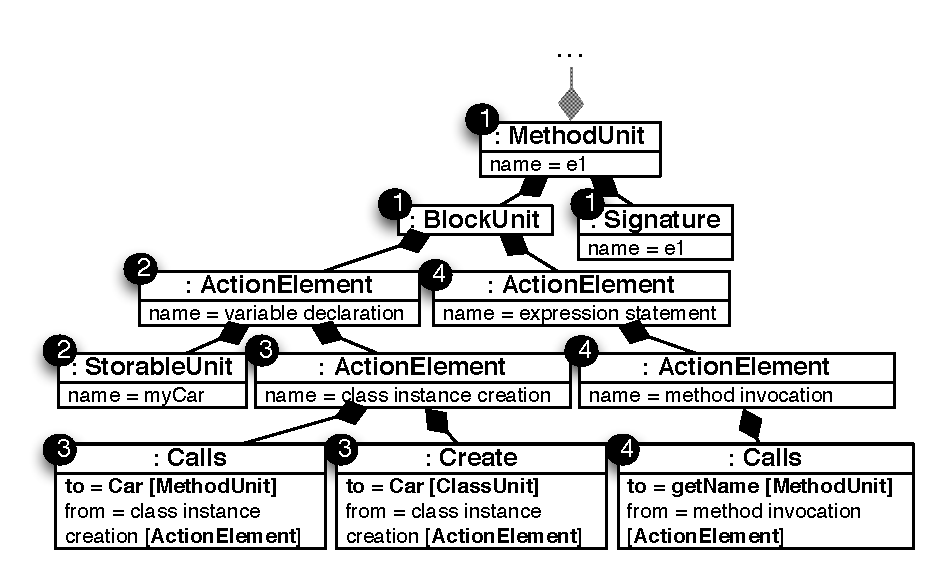
\includegraphics[scale=0.6]{images/actionInstanceKDM_2}
	\fautor
	\label{fig:kdm_instance_Java_action}
\end{minipage}

As três primeiras metaclasses mostradas nesta hierarquia são~$\mathtt{MethodUnit}$,~$\mathtt{BlockUnit}$ e~$\mathtt{Signature}$ conforme destacado na  Figura~\ref{fig:kdm_instance_Java_action} \ding{202}. Essas três metaclasses basicamente representam uma declaração e a assinatura de um determinado método, no caso \texttt{e1()}. Mais especificamente, a metaclasse~$\mathtt{MethodUnit}$ é usada para representar o método~$\mathtt{e1()}$ como mostrado tanto no Código-fonte~\ref{lst:example_kdm_instance_2} \ding{202} e na Figura~\ref{fig:kdm_instance_Java_action} \ding{202}.~$\mathtt{BlockUnit}$ representa blocos lógicos e físicos relacionados de~$\mathtt{ActionElement}$, ou seja, o escopo do método representado por \{...\}. Por sua vez,~$\mathtt{Signature}$ representa a assinatura do método, isto é, essa metaclasse representa além do nome do método todos os parâmetros, o retorno do método, exceções, etc.	

%The first three metaclasses shown in this hierarchy are the \texttt{MethodUnit}, \texttt{BlockUnit}, and \texttt{Signature} (see Figure~\ref{fig:kdm_instance_Java_action} \ding{202}). These metaclasses are used to represent a simple method declaration. More specifically, the meta-class \texttt{MethodUnit} is used to represent the method \texttt{e1} as shown in both Listing~\ref{lst:example_kdm_instance_2} \ding{202} and Figure~\ref{fig:kdm_instance_Java_action} \ding{202}. \texttt{BlockUnit} represents logically and physically related blocks of \texttt{ActionElement}, i.e., the area between the braces, \texttt{\{\ldots\}}. In turn, \texttt{Signature} represents the concept of a method signature, i.e., it also can be used to represent the name of the method, all the parameters, the return of the method, etc.

Na Linha 12 do Código-fonte~\ref{lst:example_kdm_instance_2} \ding{203} uma variável chamada~$\mathtt{myCar}$ é declarada. As metaclasses que representam esta declaração podem ser visualizadas na Figura~\ref{fig:kdm_instance_Java_action} \ding{203}. A metaclasse~$\mathtt{ActionElement}$ representa o significado das operações, por exemplo, um declaração da variável. A metaclasse~$\mathtt{StorableUnit}$ representa a própria variável, \texttt{myCar}. Ainda na Linha 10 \ding{204} a instância da classe~$\mathtt{Car}$ é criada usando a palavra-chave~$\mathtt{new}$. Nota-se que na Figura~\ref{fig:kdm_instance_Java_action} \ding{204} três metaclasses são utilizadas para representar o operador~$\mathtt{new}$. Primeiramente, a metaclasse~$\mathtt{ActionElement}$ é usada para ilustrar o significado da operação, neste caso, a instância da classe \texttt{Car}. A metaclasse~$\mathtt{Calls}$ é usada para ilustrar a instanciação de um objeto, neste caso, o objeto~$\mathtt{Car}$. Adicionalmente, a metaclasse \texttt{Calls} posssui duas ~$\mathtt{to}$ e~$\mathtt{from}$, as quais representam a chamada para o construtor de~$\mathtt{Car}$ e representa o alvo~$\mathtt{ActionElement}$, respectivamente. Em seguida, a metaclasse~$\mathtt{Creates}$ representa a nova instância de~$\mathtt{Car}$.

%In Line 10 of the Listening~\ref{lst:example_kdm_instance_2} \ding{203} a variable named \texttt{myCar} is declared. The corresponding metaclasses representing this variable declaration can be visualized in Figure~\ref{fig:kdm_instance_Java_action} \ding{203}. The meta-class \texttt{ActionElement} represents the meaning of the operations, i.e., ``variable declaration''. The \texttt{StorableUnit} represents the variable itself. Still in Line 10 \ding{204} the instance of the class \texttt{Car} is created by using the keyword \texttt{new}. Note that in Figure~\ref{fig:kdm_instance_Java_action} \ding{204} three metaclasses are used to illustrate the operator \texttt{new}. Firstly, the meta-class \texttt{ActionElement} is used to illustrate the meaning of the operation, in this case ``class instance creation'' . Secondly, the meta-class \texttt{Calls} is used to illustrate the instantiation of an object, herein \texttt{Car} object. Its owns two association, i.e., \texttt{to} and \texttt{from} which illustrates the call to the constructor of \texttt{Car} and represents the target \texttt{ActionElement}, respectively. Thirdly, the meta-class \texttt{Creates} represents the new instance of the \texttt{Car}.

Na linha 11 do Código-fonte~\ref{lst:example_kdm_instance_2} \ding{205} um método acessor é invocado. Como pode ser visto na Figura~\ref{fig:kdm_instance_Java_action} \ding{205}, três metaclasses são utilizadas no KDM para representar esta linha. Em primeiro lugar, é criado uma metaclasse~$\mathtt{ActionElement}$ que representa a declaração em si. Em seguida, outro~$\mathtt{ActionElement}$ é criado para representar a invocação de método. Finalmente, outra metaclasse~$\mathtt{Calls}$ é instânciada para representar a chamada do método~$\mathtt{getName()}$.

\subsection{Pacote \textit{Structure}}\label{sec:structurePackage}

O KDM define metaclasses que representam componentes arquiteturais, como subsistemas, camadas, componentes, etc., e define também a rastreabilidade desses elementos para outras metaclasses do KDM para o mesmo sistema por meio do pacote \texttt{Structure}.

\begin{figure}[h]
	\centering
	% Requires \usepackage{graphicx}
	\caption{Diagrama de classes do pacote \texttt{Structure}\label{fig:structureModel}}
	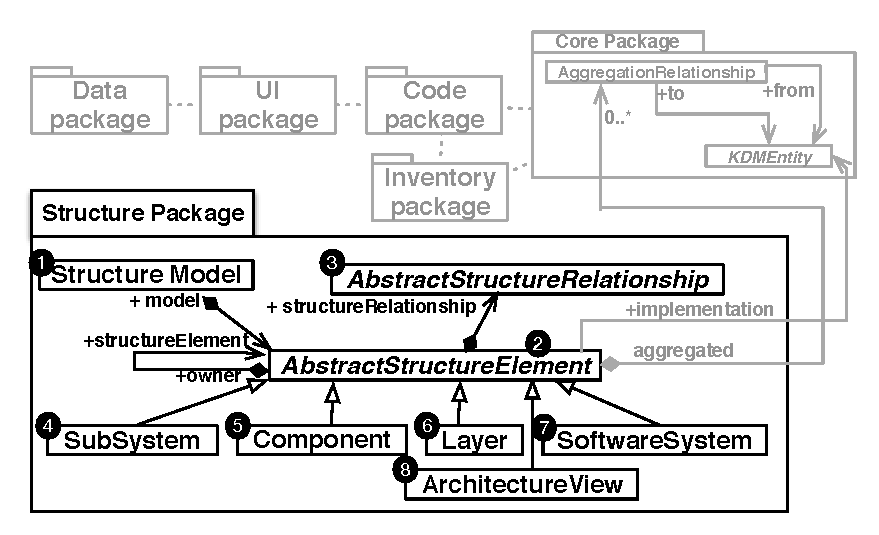
\includegraphics[scale=0.67]{images/StructurePackageFigure}
	\fadaptada{ADM:OMG}
\end{figure}

Esse pacote define um ponto de vista arquitetural para um domínio estrutural. As visões de arquitetura com bae no ponto de vista definido pelo pacote \texttt{Strcuture} representam a forma como os elementos estruturais do sistema de software estão relacionados como os módulos definidos em código-fonte, que correspondem ao pacote \texttt{Code} do KDM. Uma parte simplória do pacote \texttt{Structure} é apresentada na Figura~\ref{fig:structureModel} como um diagrama de classes.

 Usando suas metaclasses é possível relacionar todos os elementos estruturais do sistema, juntamente com os elementos computacionais, isto é, pode-se especificar os elementos estruturais do sistema. Na Figura~\ref{fig:structureModel} é mostrado que o pacote \texttt{Structure} e suas metaclasses são usadas em combinação com os pacotes \texttt{Code}, \texttt{Data}, \texttt{Platform}, \texttt{UI} e \texttt{Inventory}. O modelo \texttt{Structure} possui uma coleção de elementos estruturais, como pode ser visto na Figura~\ref{fig:structureModel} \ding{202}, isso é representado por meio de uma associação. Pacotes (do modelo \texttt{Code}) são os elementos folha do modelo \texttt{Structure}, representando a divisão de um sistema em módulos \texttt{Code} discretos, com partes não sobrepostas. A metaclasse \texttt{SoftwareSystem} fornece um ponto de encontro para todos os pacotes do sistema direta ou indiretamente através de outra associação chamada de \texttt{AbstractStructureElement[0..*]}. Os pacotes podem ainda ser agrupados nas metaclasses \texttt{SubSystem},\texttt{Layer},\texttt{Component} e \texttt{ArchitectureView}. 
 
A metaclasse \texttt{AbstractStructureElement} (conforme a Figura~\ref{fig:structureModel} \ding {203}) representa uma parte arquitetural, relacionada com a organização do sistema de software existente em módulos e possui quatro associações. A primeira associação representa os elementos pertencentes ao modelo e é chamada de $\mathtt{structureElement}$ $\mathtt{:AbstractStructureElement[0..*]}$. Em seguida, há a associação~$\mathtt{structureRelationship}$ $\mathtt{:AbstractStructureRelationship[0..*]}$, ela é usada para representar todas os relacionamentos em nível arquitetural. A associação $\mathtt{aggregated:}$ $\mathtt{AggregatedRelationship[0..*]}$ representa uma relação abstrata entre dois elementos do KDM, dentro dela é possível definir relações concretas. A última associação da metaclasse~$\mathtt{AbstractStructureElement}$ é o~$\mathtt{implementation:KDMEntity[0..*]}$. Esta associação é usada para especificar os elementos computacionais (do pacote~$\mathtt{Code}$, ou seja, $\mathtt{Package}$, $\mathtt{ClassUnit}$, $\mathtt{InterfaceUnit}$, etc) que representam o elemento estrutural. 

Na Figura~\ref{fig:kdm_structureExample} é descrita uma possível arquitetura mostrada para ilustrar como o KDM pode ser utilizado para representar elementos arquiteturais. Pode ser observado que esta figura é dividida em três níveis para ilustrar como o pacote~$\mathtt{Structure}$ está relacionado com o pacote~$\mathtt{Code}$. O nível mais baixo representa o código-fonte, artefatos físicos. L1 e L2 representam pacotes em código-fonte - cada caixa dentro dos pacotes representa as suas classes e interfaces, também é possível perceber que essas classes e interfaces são relacionados uns com os outros de alguma maneira. No meio há metaclasses do pacote~$\mathtt{Code}$, o que significa que as instâncias dessas meta -classes são usadas para representar os artefatos de baixo nível, ou seja, instâncias de~$\mathtt{Package}$ são usadas para representar L1 e L2 e instâncias de~$\mathtt{ClassUnit}$ e~$\mathtt{InterfaceUnit}$ são usados para representar as classes e interfaces, respectivamente. Finalmente, no nível superior a arquitetura é mostrada. Todos os elementos arquiteturais são representados com a seguinte padronização: a metaclasse que representa o elemento arquiteturais, ':' seguido pelo seu nome. A arquitetura apresentada é dividida da seguinte forma: no ponto mais alto de abstração há um~$\mathtt{SoftwareSystem}$ ($\mathtt{S1}$) \ding {202}, que é dividido em duas camadas, ~$\mathtt{Layer}$~$\mathtt{L1}$ \ding {203} e ~$\mathtt{Layer}$~$\mathtt{L2}$ \ding {204}. Tais camadas representam elementos arquiteturais correspondentes aos pacotes L1 e L2 representadas no nível mais baixo. A~$\mathtt{Layer}$~$\mathtt{L1}$ pode acessar os elementos da~$\mathtt{Layer}$~$\mathtt{L2}$, essa restrição \aspas{pode acessar} é representada pela metaclasse~$\mathtt{AggregatedRelationship}$ \ding {205}. Além disso, a~$\mathtt{Layer}$~$\mathtt{L2}$ contém dois componentes,~$\mathtt{C1}$ \ding {206} e~$\mathtt{C2}$ \ding {207}. Finalmente, o~$\mathtt{Component}$~$\mathtt{C1}$ fornece recursos através de uma interface para o~$\mathtt{Component}$~$\mathtt{C2}$.

\noindent \begin{minipage}{.47\textwidth}
	\centering
	\captionof{figure}{Exemplo de uma Arquitetura.}
	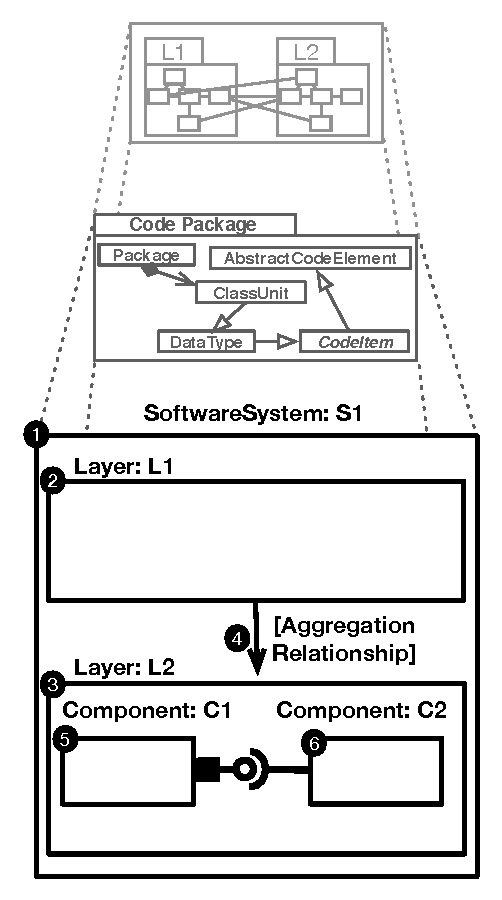
\includegraphics[scale=0.7]{images/StructureExample}
	\fautor
	\label{fig:kdm_structureExample}
\end{minipage}\hfill
\begin{minipage}{.55\textwidth}
	\centering
	\captionof{figure}{Instância KDM correspondente a Figura~\ref{fig:kdm_structureExample}}
	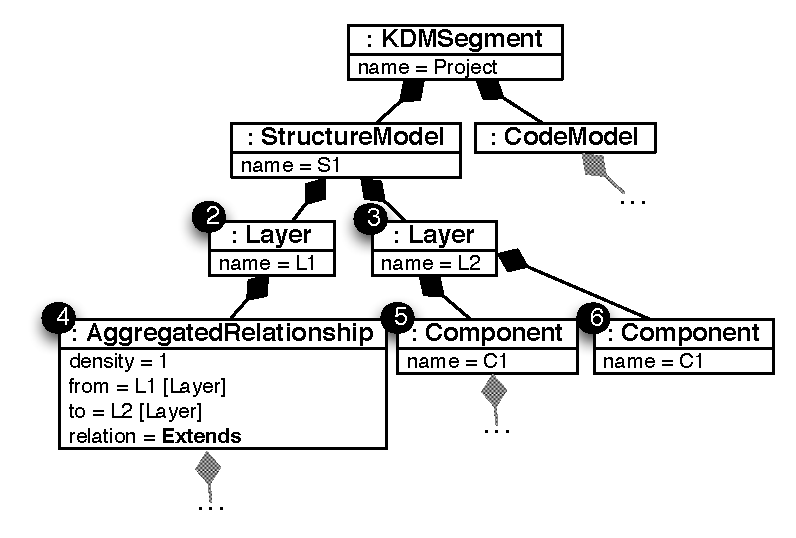
\includegraphics[scale=0.67]{images/StructureKDMINstance}
	\fautor
	\label{fig:kdm_instance_StructureExample}
\end{minipage}


O correspondente, porém simplificado da instância KDM é mostrado na Figura~\ref{fig:kdm_instance_StructureExample}. Os diamantes destacadas em cinza e em anexo com três pontos (\ldots) ilustram que algumas metaclasses não são mostrados de forma a simplificar a figura. Todos os elementos arquiteturais são subclasses de~$\mathtt{StructureModel}$. As camadas são representados pela metaclasse~$\mathtt{Layer}$, como pode ser visto na Figura~\ref{fig:kdm_instance_StructureExample} \ding{203} e \ding{204}. Da mesma forma, os componentes são representados pela metaclasse~$\mathtt{Component}$. A metaclasse mais importante a se destacar nesta figura é $\mathtt{AggregatedRelationship}$. Ela representa a relação entre a $\mathtt{Layer}$ $\mathtt{L1}$ e a $\mathtt{Layer}$ $\mathtt{L2}$. Ela possui meta atributos que tem como objetivo fornecer informações sobre o relacionamento. Por exemplo, o meta atributo~$\mathtt{density}$ ilustra o número de relações primitivas entre estas camadas. Na Figura~\ref{fig:kdm_instance_StructureExample}, o meta atributo~$\mathtt{density}$ possui o valor 1 (um). Outros dois meta atributos são o~$\mathtt{from}$ e o~$\mathtt{to}$, que representam os elementos arquiteturais de origem e destino, respectivamente. Eles são usados para especificar que a~$\mathtt{Layer}$~$\mathtt{L1}$ em~$\mathtt{SoftwareSystem}$~$\mathtt{S1}$ pode acessar a~$\mathtt{Layer}$~$\mathtt{L2}$ também em~$\mathtt{SoftwareSystem}$~$\mathtt{S1}$ de alguma forma. Finalmente, o meta atributo~$\mathtt{relation}$ representa como a~$\mathtt{Layer}$~$\mathtt{L1}$ pode acessar a~$\mathtt{Layer}$~$\mathtt{L2}$, neste contexto, através de herança usando a metaclasse~$\mathtt{Extends}$. Na Figura~\ref{fig:relationship_example_1} é mostrado como as relações entre dois elementos arquiteturais são considerados neste estudo.

\begin{figure}[!ht]
	\centering
	\caption{Relacionamento entre dois elementos arquiteturais}
	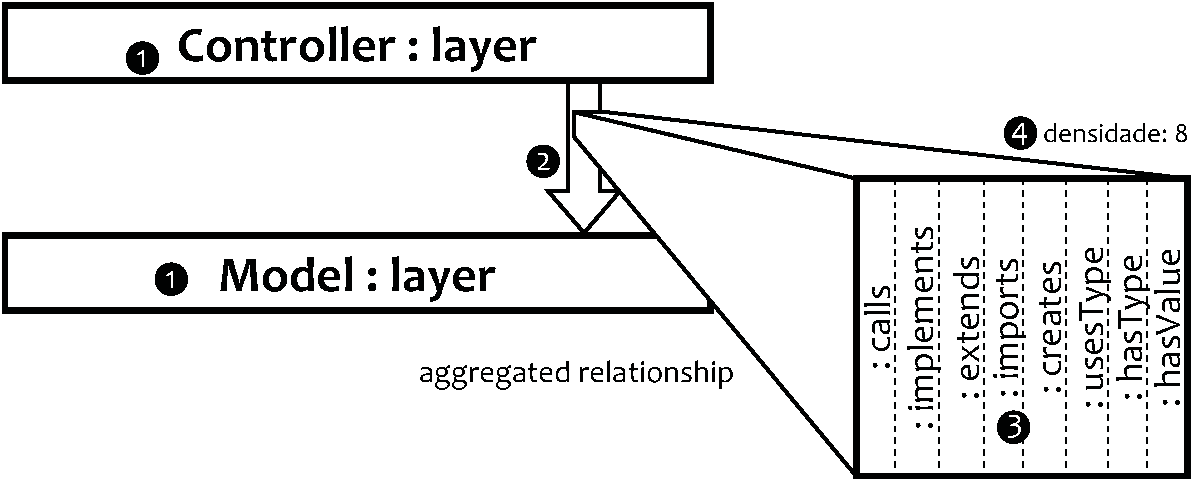
\includegraphics[width=3.3in]{images/relationshipExample1.pdf}
	\fautor
	\label{fig:relationship_example_1}
\end{figure}


Em \ding{202} os elementos arquiteturais são apresentados, camadas~$\mathtt{Controller}$ e~$\mathtt{Model}$. Como visto anteriormente, um relacionamento em nível arquitetural acontece entre dois elementos em nível estrutural (camadas, componentes, subsistemas, etc). Por exemplo, em \ding{203} é mostrando um~$\mathtt{aggregatedRelationship}$ contendo todos os possíveis relacionamentos \ding{204} entre dois elementos (chamadas de métodos, herança, etc). A seta \ding{206} representa o fluxo de entrada e saída dos relacionamentos, em outras palavras, esses relacionamentos representam as possíveis restrições iniciando na camada~$\mathtt{Controller}$  para a camada~$\mathtt{Model}$. Finalmente, a densidade \ding{205} é setada como oito, que representa o número total de relacionamentos possíveis.


\section{Ferramenta de apoio ao KDM}\label{sec:Ferramenta_de_apoio_KDM_capitulo}

Um dos trabalhos mais importantes publicados no contexto da ADM é o de~\citeonline{Bruneliere_2010MODISCO, Bruneliere_2014} que propõe uma ferramenta chamada MoDisco. MoDisco é uma framework genérico e extensível para a abordagem de Engenheria Reversa dirigida a modelos e foi implementada no \sigla{IDE}{\textit{Integrated Development Environment}} Eclipse como um \textit{plug-in}. Mais especificadamente, MoDisco é construido utilizando o \textit{Eclipse Modeling Framework} (EMF). Basicamente essa ferramenta é capaz de recuperar o código-fonte legado, base de dados e outros artefatos legado e representá-los com o metamodelo KDM. Um dos principais objetivos da ferramenta MoDisco é ser adaptável para diferentes cenários, facilitando assim a sua utilização por uma base de usuários potencialmente maior~\cite{Bruneliere_2014}. Inicialmente criado como um modelo experimental de investigação pela Equipe AtlanMod (\sigla{EMN}{\textit{Ecole des mines de Nantes}} \& \sigla{INRIA}{\textit{Institut National de Recherche en Informatique et en Automatique}}), o projeto evoluiu para uma solução industrializados graças à colaboração com a empresa MIA-Software. Este trabalho conjunto ativo resultou em um conjunto eficiente e utilizável de ferramentas para a descoberta, consulta e manipulação de modelos de software para auxiliar toda a atividade de engenharia reversa.

MoDisco tem como objetivo representar uma grande variedade de artefatos (por exemplo, código-fonte, banco de dados, arquivos de configuração, documentação, etc.) de um sistema legado. Contudo, uma das limitações dessa ferramenta é o suporte e a aplicação de refatorações. Observe que, naturalmente, MoDisco não é capaz de aplicar refatorações de forma automática, pois a maioria das refatorações necessitam de interação do usuário para fornecer as informações necessárias. No contexto desta Tese foi utilizado a ferramenta MoDisco para recuperar as informações do código-fonte legado escrito em Java. Sem o auxílio dessa ferramenta todo o sistema legado, escrito em Java, deveria ser transformada em uma instância do KDM de forma manual, o que poderia atrasar esta pesquisa, uma vez que toda a manipulação do KDM foi possível por causa da existência do MoDisco e do seu suporte em Java para manipular o metamodelo KDM. Por exemplo, não é possível para o MoDisco adivinhar quais refatorações devem ser aplicadas e em quais elementos; tais informações devem ser fornecidas por um usuário.


%\begin{figure}[!ht]
%	\centering
%	\caption{Visão geral de um projeto MoDisco.}
%	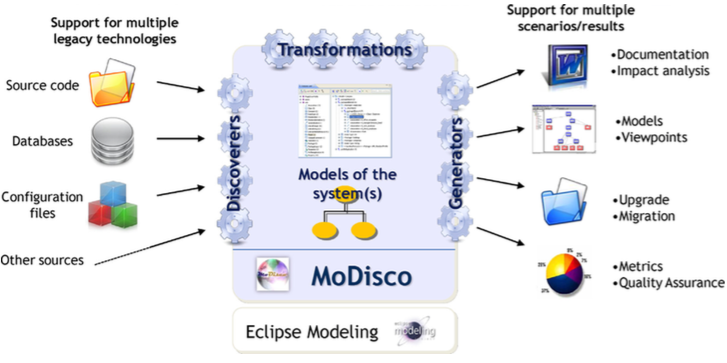
\includegraphics[scale=0.55]{images/modiscoAllArtefacts.png}
%	\label{fig:modisco_allArtefacts}
%	\fadaptada{Bruneliere_2014}
%\end{figure}


\section{Considerações Finais}\label{capitulobaclCOnsideracoesFinais}

Neste capítulo foi apresentada uma revisão dos principais conceitos envolvendo engenharia dirigida por modelos, refatoração, ADM e KDM que são relevantes para a proposta desta Tese. 

Foram discutidas e apresentadas todas as etapas que devem ser realizadas para a condução da engenharia dirigida por modelos, ou seja, todos os níveis CIM, PIM e PSM foram apresentados. Em seguida, foi apresentada a definição e diferença de metametamodelo, metamodelo, modelo e dados. Posteriormente, transformações em modelos foram apresentadas e discutidas, salientando as principais classificações relacionadas a transformações encontradas na literatura - vertical ou horizontal; endógenas ou exógenas. Ainda em relação à transformação de modelos, algumas das principais linguagens utilizadas para realizar a transformação em modelos também foram apresentadas. Porém, apenas a linguagem ATL foi discutida com maiores informações. Os principais conceitos relacionados com refatoração também foram apresentados.


Além disso, este capítulo direciona-se à análise do panorama atual da literatura que trata sobre a modernização de sistemas legados levando em consideração a padronização proposta pelo OMG. Assim, foram mostrados os principais conceitos sobre ADM, KDM, bem como seus pacotes e camadas que são necessários para facilitar o entendimento dessa Tese e também são fundamentais para o desenvolvimento da proposta aqui desenvolvida.

Observou-se também que o metamodelo KDM por intermédio de suas camadas, pacotes e metaclasses permite a criação de um modelo independente de plataforma que representam um sistema em diversas visões. O objetivo do OMG ao criar esse metamodelo é propor uma padronização da reengenharia de software, fornecendo abstrações que ajudem no processo de reengenharia de sistemas. Além disso, pode-se constatar que diferentemente de metamodelos existentes, tais como a UML, o KDM tem como intuito agrupar todos os artefatos (visões) do sistema em um único metamodelo. Dessa forma, pode-se argumentar que o metamodelo KDM pode ser considerado como uma família de metamodelos, uma vez que o mesmo compartilha uma terminologia consistente e homogenia.

Finalmente, este capítulo também apresentou MoDisco, uma das principais ferramentas que automatiza a instanciação do metamodelo KDM. Essa ferramenta foi utilizada no contexto deste trabalho para dar suporte à recuperação de instâncias do metamodelo KDM a partir de código-fonte escrito em Java. No próximo capítulo é apresentado um mapeamento sistemático sobre ADM e KDM que foi conduzido para identificar possíveis desertos de evidências.


%\chapter{Modernização Orientada à Arquitetura e KDM}
%\label{chapter:adm_kdm}
%
\section{Considerações Iniciais}

Este capítulo apresenta uma abordagem conceitual da modernização de sistemas e os esforços da OMG para a realização de uma padronização em nível de modelo desses sistemas. O escopo do trabalho é delimitado e se discute especificadamente sobre Modernização Orientada à Arquitetura (do inglês - \textit{Architecture-Driven Modernization} - ADM) e \textit{Knowledge Discovery metamodel} (KDM). ADM é o processo de modernização apoiado por modelos da OMG que utiliza os conceitos da MDE. Neste capítulo, são abordados os principais pontos dessa modernização, bem como é apresentada uma descrição mais detalhada do seu principal metamodelo, que é o KDM. Esse capítulo fornece a base necessária para realizar e entender refatorações em nível de modelo, mais especificadamente no metamodelo KDM.

\section{Modernização Orientada à Arquitetura} 

O crescente interesse na MDE motivou a \sigla{OMG}{\textit{Object Management Group}} a lançar a iniciativa denominada Modernização Dirigida à Arquitetura (do inglês - \textit{Architecture-Driven Modernization} (ADM)), cujo objetivo foi estabelecer metamodelos padronizados para auxiliar todo o  processo da reengenharia de software. Tal iniciativa foi motivada devido ao alto número de projetos reengenharia de software que não obtiveram sucesso~\cite{Sneed_2005, Demeyer2}. Como resultado desse esforço os conceitos da ADM foram criados, os quais possuem como objetivo revitalizar/modernizar softwares existentes\footnote{No contexto desse documento softwares existentes e sistemas legados são utilizados de forma intercambiáveis} com a utilização de metamodelos padronizados empregando os princípios da abordagem Arquitetura Dirigida à Modelo (do inglês - \sigla{MDA}{\textit{Model-Driven Architecture}}) (ver Seção~\ref{Cap2_Sec2_Desenvolvimento_Dirigido_a_Modelos}). %No contexto da ADM, todos os modelos são homogêneos, permitindo assim a criação de transformações \textit{Model-To-Model} M2M 

De acordo com a OMG~\cite{OMG_OMG} o objetivo da ADM não é substituir o processo tradicional da reengenharia de software, pelo contrário, a ADM tem como objetivo auxiliar e melhorar o processo de reengenharia de software por meio da utilização dos princípios da MDA. A ADM consiste em uma adaptação do modelo de ferradura tipicamente conhecido em reengenharia de software (i.e, o modelo de ferradura, basicamente contêm dois lados, esquerdo, direito e uma \aspas{ponte} ligando os dois lados). Na Figura~\ref{fig:horse_shoe} é apresentado o modelo de ferradura adaptado para a ADM. É importante observar que essa figura contêm todas as fases e \aspas{palavras-chaves} tradicionais que são encontradas na reengenharia de software tradicional e em MDA, tais como: Modelo Especifico de Plataforma (do inglês - \sigla{PSM}{\textit{Platform-Specific Model}}), Modelo Independente de Plataforma (do inglês - \sigla{PSM}{\textit{Platform-Independent Model}}) e Modelo Computacional Independente (do inglês - \sigla{CIM}{\textit{Computation-Independent Model}}). As fases tradicionais da reengenharia de software adaptadas para a ADM são:


\begin{itemize}
 	\item \textbf{Engenharia Reversa}: Esta fase têm como entrada um sistema que será modernizado, posteriormente esse sistema é transformado em um PSM. Além disso, o PSM é utilizado como entrada para a geração do PIM, que no contexto dessa tese consiste em uma instância do metamodelo denominado KDM (ver Seção~\ref{sec:knowledge_discovery_meta_model}) que será explicado com mais detalhes posteriormente;
 	\item \textbf{Reestruturação}: Nesta fase um conjunto de reestruturação/refatoração podem ser aplicadas sobre uma instância do metamodelo KDM por meio de transformações de modelo para modelo (do inglês - \sigla{M2M}{\emph{Model-To-Model}});
 	\item \textbf{Engenharia Avante}: Nesta fase um novo código-fonte do sistema modernizado é gerado automaticamente por meio de transformações de modelo para código (do inglês - \sigla{M2C}{\emph{Model-To-Code}}). 
 \end{itemize} 

 \begin{figure}[htb]
 \caption{Modelo de ferradura adaptada para a ADM}
 \label{fig:horse_shoe}
 \centering
 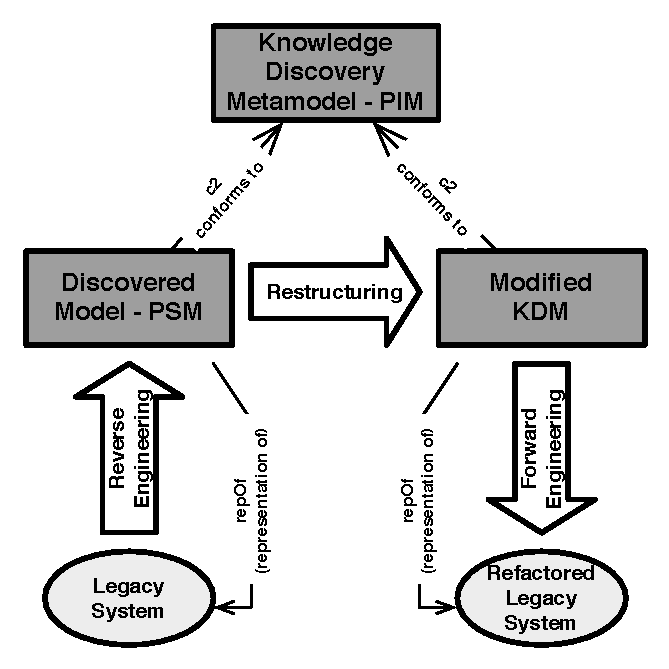
\includegraphics[scale=0.8]{images/horseshoes.pdf}
 \fadaptada{ADM:OMG}
\end{figure}

Como ressaltado anteriormente, durante todo o processo da ADM todos os modelos (i.e., PSM, PIM e CIM) podem estabelecer transformações/refatorações entre si, como ilustrado na Figura~\ref{fig:horse_shoe}. Geralmente tais transformações são executadas por meio de linguagens de transformações. Como salientado no Capítulo~\ref{chapter:fundamentacao_teorica}, Seção~\ref{sec:transformacoes_de_modelos} usualmente essas transformações são implementadas utilizando diferentes linguagens de transformações que podem ser declarativas, imperativas ou híbridas. 

É importante também destacar que a ADM não tem como intuito apenas seguir todos os princípios da abordagem MDA~\cite{ADM:OMG}. Um dos principais objetivos da ADM é definir um conjunto de metamodelos, padronizados, para lidar com diferentes desafios que são encontrados durante a reengenharia de software. Dessa forma, em Novembro de 2003, a \sigla{ADMTF}{\textit{Architecture-Driven Modernization Task Force}} criou uma \sigla{RFP}{\textit{Request-for-Proposal}} que por sua vez descrevia um conjunto de metamodelos, tais metamodelos são: (\textit{i}) \sigla{KDM}{\textit{Knowledge Discovery metamodel}}, maiores informações sobre esse metamodelo é apresentado na seção~\ref{sec:knowledge_discovery_meta_model}, (\textit{ii}) \sigla{SMM}{\textit{Structured Metrics metamodel}} que é um metamodelo para representar e definir métricas e resultados de medições, (\textit{iii}) \sigla{ADMPR}{\textit{ADM Pattern Recognition}}, que facilita a busca de padrões em um softare, (\textit{iv}) \sigla{ADMVS}{\textit{ADM Visualization Specification}}, que tem como objetivo representar visualmente metadados de uma aplicação representada em KDM, (\textit{v}) \sigla{ADMRS}{\textit{ADM Refactoring Specification}}, que almeja definir um metamodelo padronizado para especificar e definir refatorações utilizando outros metamodelos da ADM, como por exemplo o KDM. O estado atual de cada metamodelo pode ser visto na Tabela~\ref{tab:todos_os_meta_modelos_da_ADM}~\cite{ADM:OMG}. É de suma importância destacar que alguns metamodelos ainda encontram-se em fase de desenvolvimento e outros já foram finalizadas e disponíveis pela OMG.

% Please add the following required packages to your document preamble:
% \usepackage{multirow}
\begin{table}[]
\centering
\caption{Estado atual dos metamodelos da ADM.}
\label{tab:todos_os_meta_modelos_da_ADM}
\begin{tabular}{|l|l|l|l|}
\hline
metamodelo                                         & Situação           & Versão & Data          \\ \hline
ADMPR (ADM Pattern Recognition)                     & Em desenvolvimento &        &               \\ \hline
ADMRS (ADM Refactoring Specification)               & Em desenvolvimento &        &               \\ \hline
ADMVS (ADM Visualization Specification)             & Em desenvolvimento &        &               \\ \hline
ASTM (Abstract Syntax Tree Metamodel)               & Disponível         & 1.0    & Janeiro/2011  \\ \hline
KDM (Knowledge Discovery Metamodel)                 & Disponível         & 1.3    & Agosto/2011   \\ \hline
\multirow{2}{*}{SMM (Structured Metrics Metamodel)} & Disponível         & 1.0    & Janeiro/2012  \\ \cline{2-4} 
                                                    & Em desenvolvimento & 1.1    & Novembro/2013 \\ \hline
\end{tabular}
\end{table}

É importante destacar que a abordagem proposta nesta Tese, se concentra no metamodelo KDM. Consequentemente, é de suma importância o entendimento desse metamodelo, por isso, esse metamodelo é mais detalhado neste capítulo.
KDM é um metamodelo que pode ser utilizado para representar todos os artefatos de um determinado software existente, por exemplo, o KDM contêm metaclasses especificas para representar desde de código-fonte até a arquitetura de um determinado software. O KDM é um metamodelo de representação intermediária comum para sistemas existentes e seus ambientes operacionais. Utilizando esse metamodelo para sistemas existentes é possível trocar representações do sistema em modelo entre plataformas e linguagens com a finalidade de analisar, padronizar e transformar/refatorar os sistemas existentes~\cite{ADM:OMG}. A ideia por trás do KDM é que a comunidade comece a criar analisadores sintáticos (do inglês \textit{parsers}) para diferentes linguagens de programação, que transforme os códigos-fontes em instâncias do metamodelo KDM. Como resultado, qualquer técnica, ferramenta, abordagem, etc, que utilize KDM como o artefato de entrada pode ser considerado uma técnicas, ferramenta, abordagem independente de linguagem e de plataforma. Por exemplo, um catálogo de refatoração para o KDM~\cite{durelli_catalogo, durelli_VEM_ferramenta} (ver Capítulo~\ref{cap:refactoring_catalogue}) pode ser utilizado para refatorar vários sistemas independentemente da linguagem de programação. Maiores informações sobre o KDM, bem como seus pacotes, metaclasses e metarelacionamentos são apresentados a seguir.

\section{Knowledge Discovery metamodel}
\label{sec:knowledge_discovery_meta_model}

\sigla{KDM}{Knowledge Discovery metamodel} é um metamodelo para representar existentes artefatos de software, seus elementos, associações, e ambientes operacionais. De acordo com~\cite{KDM:specification, PerezCastillo:2011jo, ADMCHAPTERR} o KDM tem como principal objetivo permitir que engenheiros de software criem ferramentas para auxiliar a modernização de software que sejam independente de plataforma e linguagem. Além disso, o KDM facilita e assegura a interoperabilidade e troca de dados entre diferentes ferramentas. 

Um problema tradicional facilmente identificado em várias ferramentas que lidam com a reengenharia de software é que tais ferramentas analisam diversos artefatos de um determinado software (por exemplo, código-fonte, banco de dados, \textit{scripts}, etc.) para obter conhecimentos explícitos com o intuito de realizar transformações/refatorações~\cite{rosenberg, Canfora2011}. Como consequência cada ferramenta gera e analisa tais conhecimentos de forma implícita, ou seja, os conhecimento gerados são restritos à uma especifica linguagem de programação, e/ou a uma plataforma. Como resultado tais restrições podem criar dificuldades com relação a interoperabilidade entre diferentes ferramentas. Consequentemente, o KDM fornece uma estrutura que tem com objetivo facilitar a troca de dados entre diversas ferramentas. Além disso, o KDM possui um conjunto de metaclasse e uma estrutura padronizada que fornece meios para especificar desde artefatos físicos até lógicos de um determinado sistema. Em virtude dessa padronização, todas as técnicas/abordagem/ferramentas que utilizam o KDM como entrada podem ser consideradas independente de plataforma e linguagem, aumentando assim, a interoperabilidade e o reúso. 


Pode-se sumarizar os principais objetivos do KDM como~\cite{ADM:OMG}:

\begin{itemize}
	\item KDM representa artefatos de um sistema legado como entidades, relacionamentos e atributos;
	\item KDM suporta uma  variedade de plataforma e linguagem;
	\item KDM define uma terminologia unificada para artefatos de sistemas legados;
	\item KDM representa estruturas lógicas e físicas de sistemas legados;
	\item KDM permite a modificação/refatoração de sistemas legados utilizando os princípios da MDA;
	\item KDM facilita o rastreamento de mudança entre artefatos;
	\item KDM facilita a sincronização de estruturas lógicas e físicas de um determinado sistema legado;
	\item KDM contêm metaclasses para representar desde código-fonte até metaclasses para representar elementos arquiteturais de um determinado sistema legado.
\end{itemize}

Em 2012 o KDM tornou-se \sigla{ISO}{\emph{International Standards Organization}}~\cite{KDM:ISO} como uma estrutura que facilita a troca de dados entre as diversas ferramentas. O KDM é definido via \sigla{MOF}{\emph{Meta-Object Facility}}~\cite{MOF}. Além disso, o KDM estabelece o formato de troca de dados via \sigla{XMI}{\emph{XML Metadata Interchange}}, o qual é denominado KDM XMI \emph{schema}. 


De acordo com~\citeonline{KDM:specification} e~\citeonline{PerezCastillo:2011jo} o KDM possui o objetivo de cobrir um amplo escopo, para abranger um conjunto grande e diversificado de aplicações, plataformas e linguagens de programação. Um dos principais objetivos do KDM é fornecer a capacidade de troca de metadados entre diversas ferramentas e, assim, facilitar a cooperação entre fornecedores para integrar e aumentar a interoperabilidade de diferentes abordagens, técnicas, algoritmos, etc. A fim de alcançar essa interoperabilidade e, especialmente, a integração de informações sobre diferentes facetas de um determinado sistema a partir de múltiplas ferramentas, o KDM define vários níveis de conformidade, aumentando assim a probabilidade de que duas ou mais ferramentas apoiaram o mesmo metamodelo. Além disso, o KDM também é estruturado de forma modular, seguindo o princípio da separação de interesse, com a capacidade de representar partes heterogêneas de um sistema. A separação de interesses no contexto do metamodelo KDM são alcançadas por meio de pacotes, como apresentado na Figura~\ref{kdm:domain}. Cada pacote está em um nível de conformidade e possui o objetivo de definir um ponto de vista arquitetural do sistema. Em outras palavras, cada pacote do KDM constitui uma determinada ontologia para descrever e representar a grande maioria dos artefatos de sistemas de software existentes. Por exemplo, os pacotes \texttt{Code} e \texttt{Action} definem metaclasses para representar o código-fonte de um sistema, tais como, variáveis, procedimentos/métodos/funções, chamadas para procedimentos/métodos/funções. Similarmente o pacote \texttt{Structure} contêm metaclasses para representar elementos arquiteturais do sistema, tais como, componentes, camadas, sub-componentes, etc. O pacote \texttt{Conceptual} possui  metaclasses para definir regras de negócio do sistema.


\begin{figure}[htb]
 \caption{Pacotes e nível de conformidade do metamodelo KDM.}
 \label{kdm:domain}
 \centering
 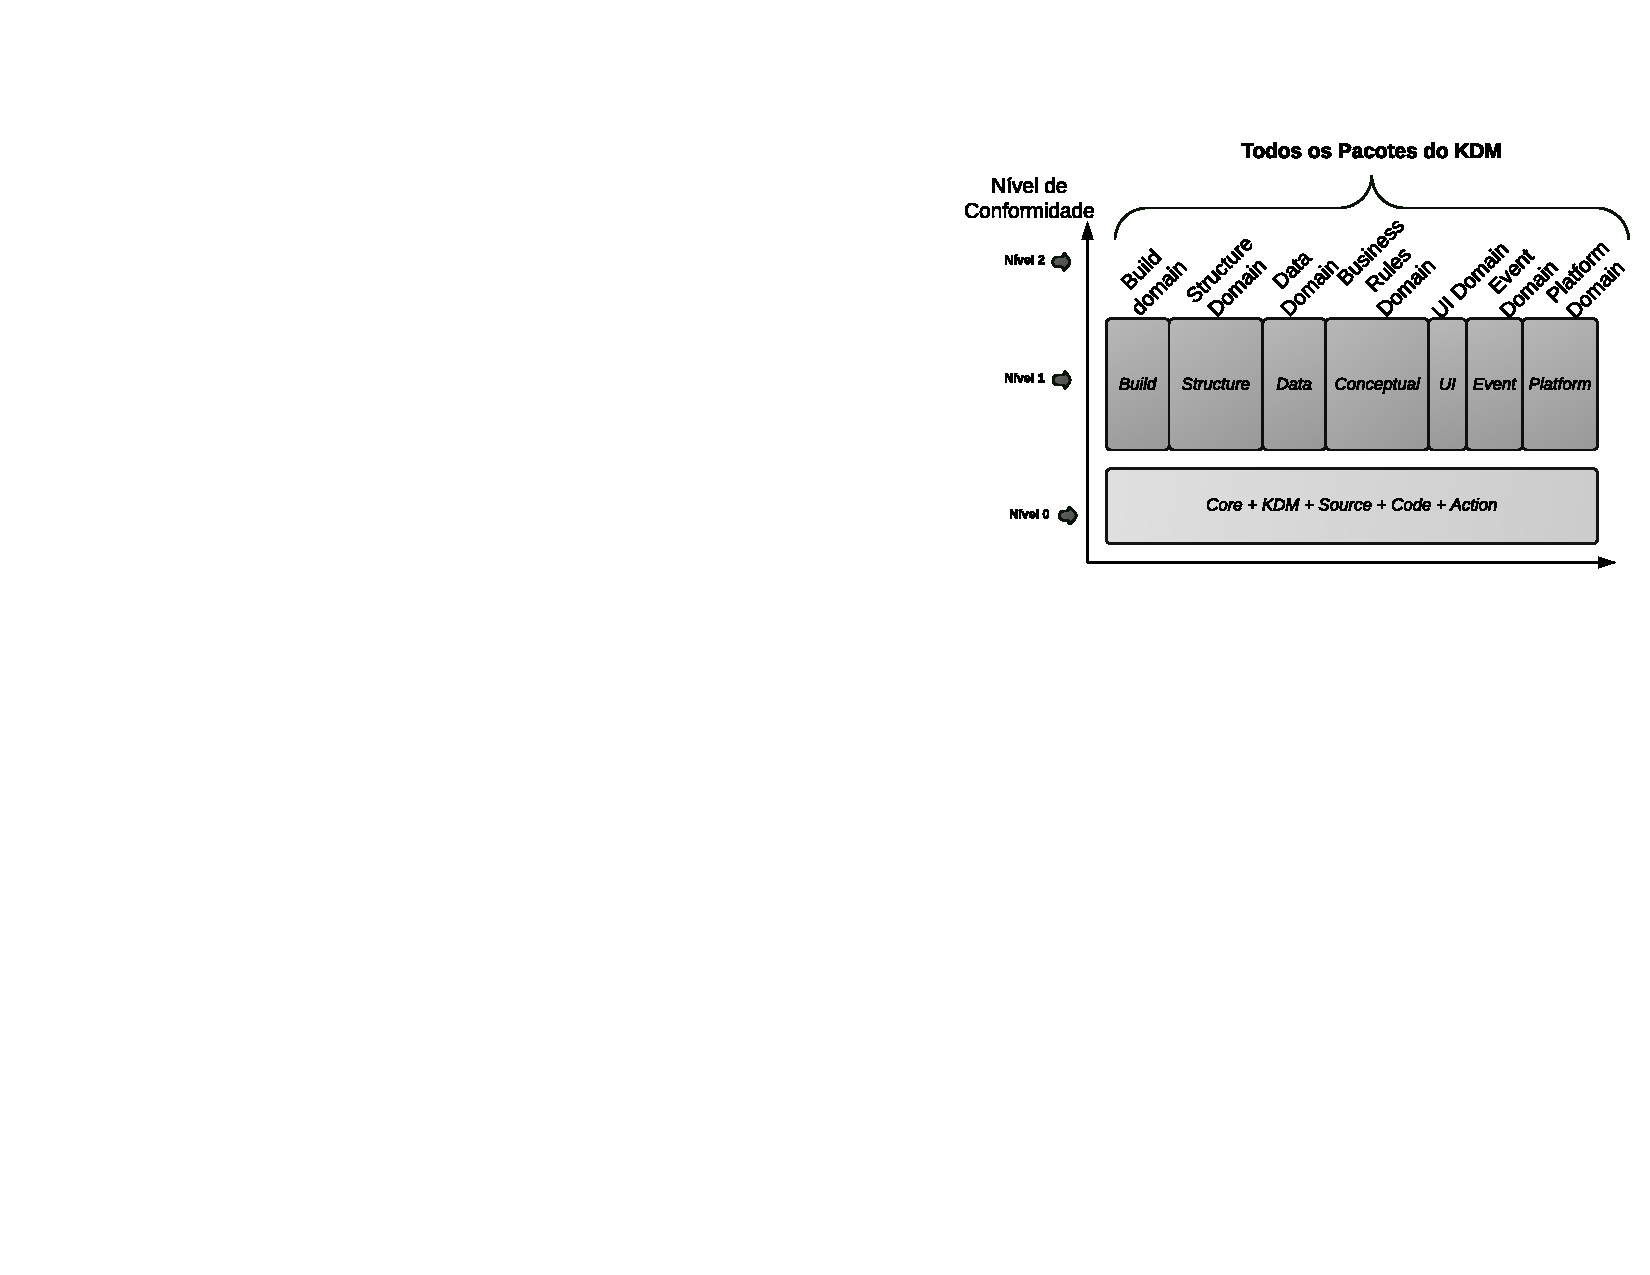
\includegraphics[scale=1]{images/kdmLevels_pacotes.pdf}
 \fadaptada{KDM:specification}
\end{figure}

Da perspectiva de um engenheiro de software, essa separação de interesse do KDM, por meio de pacote, significa que o engenheiro só precisa se preocupar com os pacotes do KDM que considerar necessários para as suas atividades de modernização, por exemplo, uma determinada abordagem pode necessitar apenas do pacote \texttt{Code} e \texttt{Action}, enquanto uma outra abordagem utilize apenas o pacote responsável por definir elementos arquiteturais. Se essas abordagens forem evoluídas ao longo do tempo e necessitarem de outros pacotes do KDM, os respectivos pacotes podem ser adicionado ao repertório da abordagem/ferramenta, conforme necessário.

Como observado na Figura~\ref{kdm:domain} o KDM possui três níveis de conformidade, nível 0, nível 1 e nível 2. Informações sobre cada nível é apresentado a seguir:

\begin{itemize}
    \item \textbf{Nível 0}: nesse nível de conformidade são definidos os seguintes pacotes do KDM: (\textit{i})     \texttt{Core}, (\textit{ii}) \texttt{kdm}, (\textit{iii}) \texttt{Source}, (\textit{iv}) \texttt{Code} e (\textit{v}) \texttt{Action}. Mais importante, esse nível de conformidade representa um denominador comum que pode servir como uma base para a interoperabilidade entre diferentes categorias de ferramentas que utilizem o metamodelo KDM. Para que uma ferramenta esteja em conformidade com o Nível 0 ela deve fornecer completo suporte para todas as metaclasses que foram definidas nos pacotes \texttt{Core}, \texttt{kdm}, \texttt{Source}, \texttt{Code} e \texttt{Action};
    \item \textbf{Nível 1}: nesse nível os pacotes definidos no Nível 0 são estendidos para representar outros artefatos de um determinado sistema. Especificamente esse nível define os seguintes pacotes: (\textit{i}) \texttt{Build}, (\textit{ii}) \texttt{Structure}, (\textit{iii}) \texttt{Data}, (\textit{iv}) \texttt{Conceptual}, (\textit{v}) \texttt{UI}, (\textit{vi}) \texttt{Event} e (\textit{vii}) \texttt{Platform}. Para que uma ferramenta esteja em conformidade com o Nível 1 ela deve fornecer suporte para pelo menos um do pacotes devido nesse nível;
    \item \textbf{Nível 2}: esse nível é a união de todos os pacotes definidos no nível anterior. Para que uma ferramenta esteja em conformidade com o Nível 2 ela deve fornecer suporte para todos os pacotes devido no Nível 1.
\end{itemize}


Posteriormente todos os pacotes do KDM são organizados em quatro camadas de abstração. Tais camadas são:

\begin{itemize}
    \item \sigla{CI}{Camada de Infraestrutura}: do inglês \textit{Infrastructure Layer};
    \item \sigla{CEP}{Camada de Elementos de Programa}: do inglês \textit{Program Elements Layer};
    \item \sigla{CRTE}{Camada de Recurso de Tempo de Execução}: do inglês \textit{Runtime Resource Layer};
    \item \sigla{CA}{Camada de Abstração}: do inglês \textit{Abstraction Layer}.
\end{itemize}


%(\textit{i}) \sigla{CI}{Camada de Infraestrutura} (do inglês \textit{Infrastructure Layer}), (\textit{ii}) \sigla{CEP}{Camada de Elementos de Programa} (do inglês \textit{Program Elements Layer}), (\textit{iii}) \sigla{CRTE}{Camada de Recurso de Tempo de Execução} (do inglês \textit{Runtime Resource Layer}) e (\textit{iv} ) \sigla{CA}{Camada de Abstração} (do inglês \textit{Abstraction Layer}). 

%Cada camada é posteriormente organizada em pacotes, como pode ser observado na Figura~\ref{fig:kdm_layer}. Por sua vez, cada pacote define um conjunto de metaclasses cujo propósito é representar o conhecimento de específicos artefatos de um determinado sistema. 

%
\begin{figure}[htb]
 \caption{Camadas e pacotes do KDM.}
 \label{fig:kdm_layer}
 \centering
 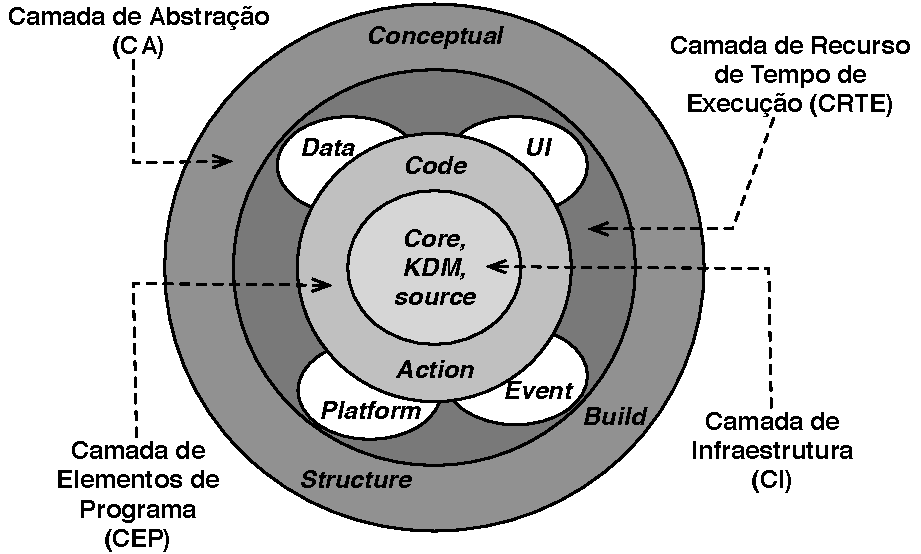
\includegraphics[scale=0.8]{images/kdm_layers.pdf}
 \fadaptada{KDM:specification}
\end{figure}
%
A CI contêm três pacotes, são eles: (\textit{i}) \texttt{Core}, (\textit{ii}) \texttt{\aspas{kdm}} e (\textit{iii}) \texttt{Source}. Os dois primeiros pacotes, \texttt{Core} e \texttt{\aspas{kdm}}, representam a infraestrutura básica para outros pacotes do KDM, ou seja, definem metaclasses e relacionamentos básicos. O pacote \texttt{Source} define o \texttt{Inventory Model}, o qual representa artefatos de software e mantêm a rastreabilidade entre eles. 

A CEP possui dois pacotes: (\textit{i}) \texttt{Code} e (\textit{ii}) \texttt{Action}. Esses pacotes coletivamente definem o \texttt{Code Model}, o qual contêm metaclasses para representar artefatos em nível de implementação. O pacote \texttt{Code} contêm um conjunto de metaclasses para representar a estrutura de um determinado programa e seus relacionamentos, enquanto que o pacote \texttt{Action} possui metaclasses para descrever o comportamento e o fluxo de dados de um programa.

A CRTE contêm quatro pacotes: (\textit{i}) \texttt{Data}, (\textit{ii}) \texttt{Platform}, (\textit{iii}) \texttt{Event} e (\textit{iv}) \texttt{UI}. Coletivamente tais pacotes representam a estrutura e comportamento de recursos de tempo de execução do sistema. Tais pacotes são diretamente instanciados por meio da definição de recursos, abstração do \texttt{Code Model}, ou são manualmente instanciado pelo engenheiro de modernização. A rastreabilidade entre os elementos abstraídos e os elementos físicos (por exemplo, código-fonte) são mantidos pelo meta-atributo denominado \texttt{implementation}. Finalmente, a CA contêm três pacotes: (\textit{i}) \texttt{Conceptual}, (\textit{ii}) \texttt{Structure} e (\textit{iii}) \texttt{Build}. Esses pacotes possuem metaclasses para representar o maior nível de abstração de um sistema, por exemplo, a estrutura do sistema, regras de negócios, documentações do sistema, etc.

\begin{figure}[htb]
 \caption{Representação das quatro camadas do KDM de um determinado sistema.}
 \label{fig:kdm_layer_sistema_completo}
 \centering
 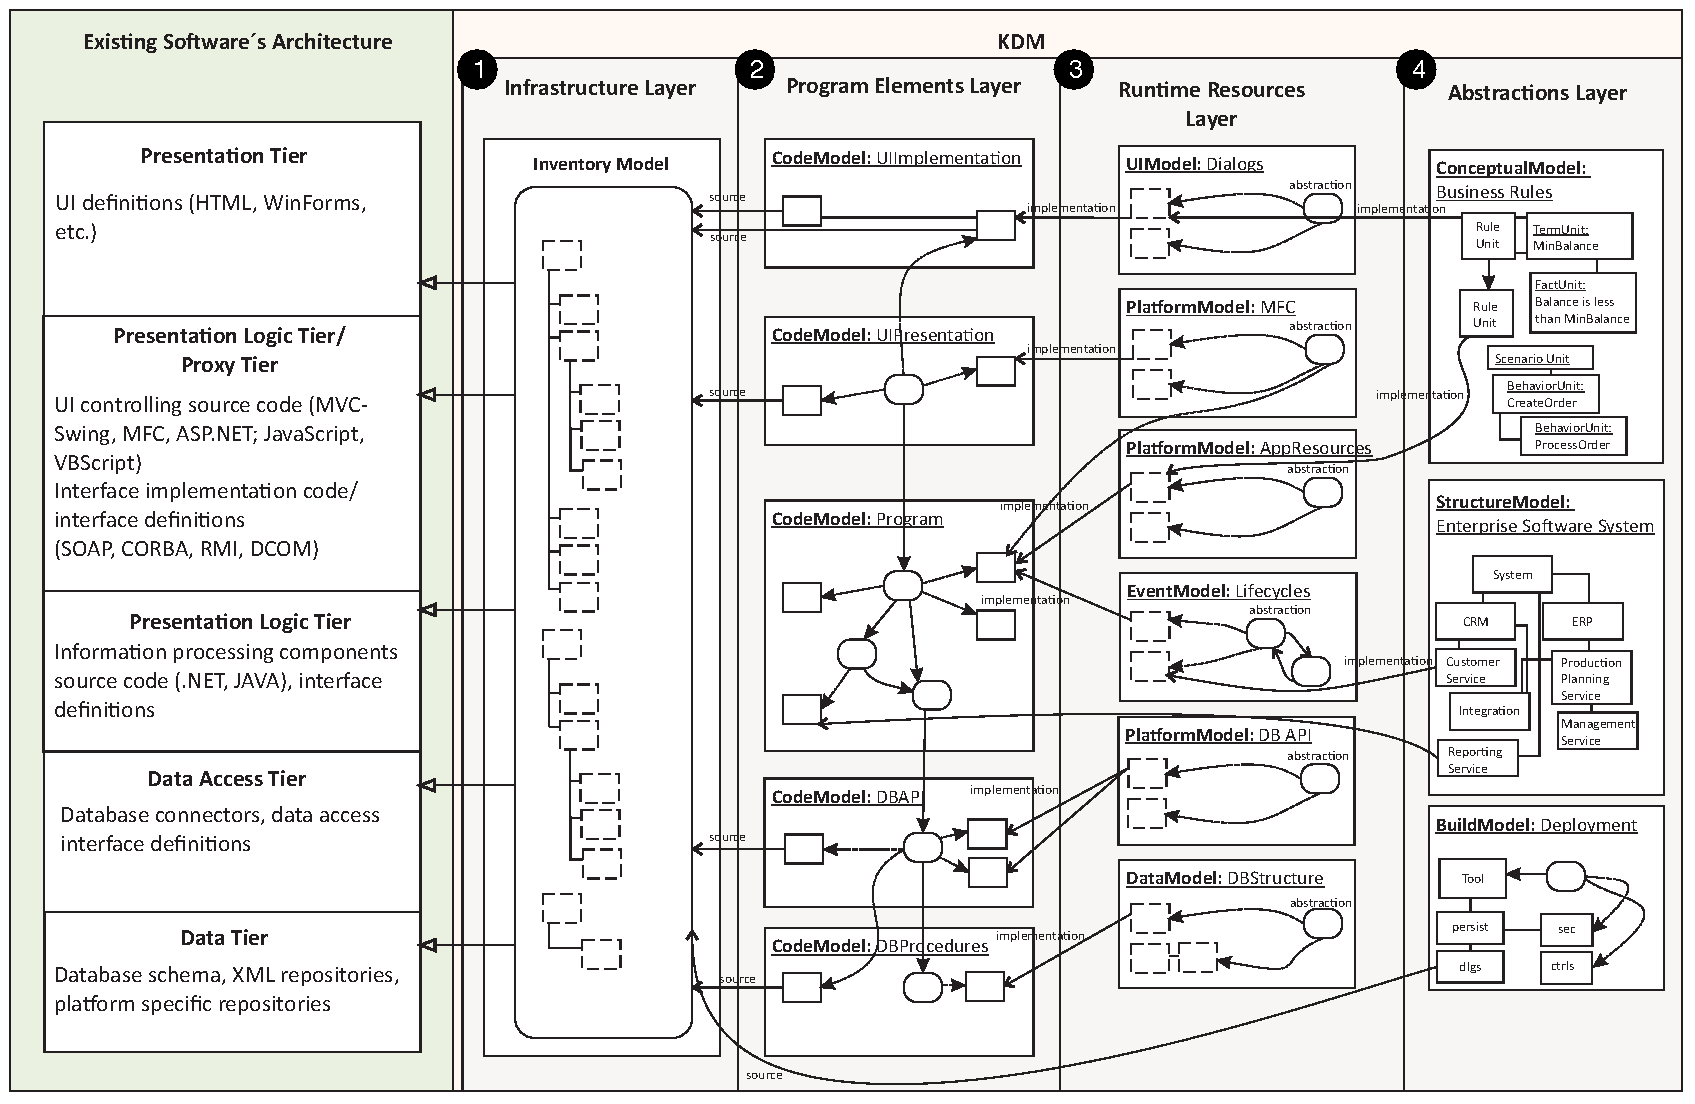
\includegraphics[scale=0.6]{images/kdm_Layer.pdf}
 \fautor
\end{figure}

Como salientado anteriormente cada camada do KDM representa diferentes perspectivas de conhecimento sobre os artefatos de sistemas. Tais camadas e/ou pacotes do KDM podem ser criados automaticamente, semi-automaticamente, ou manualmente por meio da aplicação de várias técnicas de extração de conhecimento, análises e transformação. Por exemplo, na Figura~\ref{fig:kdm_layer_sistema_completo} é apresentado uma arquitetura de software que esta dividida em várias camadas do KDM, e consequentemente utiliza vários pacotes e metaclasses para representar todos os artefatos do software. 

Essa figura pode ser analisada verticalmente e horizontalmente; verticalmente é possível identificar as quatros camadas do KDM apresentadas anteriormente: CI \ding{182}, CEP \ding{183}, CRTE \ding{184} e CA \ding{185}. Tais camadas possuem abstrações (metaclasses) dos artefatos heterogêneos que servem para funções distintas e que estão representados horizontalmente. Por exemplo, em \emph{Data Tier} é definido diferentes tipos de artefatos de bancos de dados, XML, CVS e DAT. Os componentes que realizam a conectividade com os bancos de dados (por exemplo, \sigla{ODBC}{\emph{Open Database Connectivity}} e \sigla{JDBC}{\emph{Java Database Connectivity}}) estão em \emph{Data Access tier}. Em \emph{Processing Logic tier} estão definidos os componentes que implementam regras de negócio. Além disso, também são definidos os componentes que interagem com componentes de interface com o usuário. Em \emph{Proxy tier} estão definidos artefatos que fazem iterações com elementos externos, por exemplo SOAP, DCOM, CORBA, JNI, ou RMI. Finalmente, \emph{Presentation tier} é responsável por produzir e controlar componentes gráficos, tais como, formulários, páginas \emph{web} ou relatórios. 

Uma característica importante de ser observada e ressaltada na Figura~\ref{fig:kdm_layer_sistema_completo} é que todos as camadas do KDM interagem, significando que todas as camadas são conectadas de alguma forma\footnote{Essa conectividade entre os elementos de cada camada são mantidos por um conjunto de meta-atributo, por exemplo, o meta-atributo \texttt{implementation}.}, como consequência se uma mudança/refatoração é realizada em uma camada especifica, a mudança/refatoração deve ser propagada para outras camadas com o intuito de manter todas as camadas sincronizadas e consistentes preservando assim a estrutura estática do KDM e o comportamento do código representado em KDM.

Na Tabela~\ref{tab:visao_geral_kdm} é apresentada uma visão detalhada de todas as camadas do metamodelo do KDM. Além disso, essa tabela também apresenta as técnicas que podem ser utilizadas para instanciar cada pacote do KDM. 

\begin{longtable}{ | m{2.5cm} | m{5.9cm}| m{3.5cm} | m{3.5cm} | } 
 \caption{ Visão geral das camadas do KDM e técnicas utilizadas para instanciar todos os pacotes do KDM.\label{tab:visao_geral_kdm}}\\
 
 \hline
 \multicolumn{4}{| c | }{Início da Tabela~\ref{tab:visao_geral_kdm}}\\
 \hline
 \textbf{Camadas} & \textbf{Pacotes do KDM}  & \textbf{Artefatos de Entrada} &\textbf{Técnicas}\\
 \hline
 \endfirsthead
 
 \hline
 \multicolumn{4}{|c|}{Continuação da Tabela~\ref{tab:visao_geral_kdm}}\\
 \hline
 \textbf{Camadas} & \textbf{Pacotes do KDM}  & \textbf{Artefatos de Entrada} &\textbf{Técnicas}\\
 \hline
 \endhead
 
 \hline
 \endfoot
 
 \hline
 \multicolumn{4}{| c |}{Fim da Tabela~\ref{tab:visao_geral_kdm}}\\
 \hline\hline
 \endlastfoot
 
 \hline CI & Pacotes: \emph{Code} e \emph{Action} (\emph{Code Model}) \newline - Representa aspecto estrutural e comportamental do código-fonte, ou seja, contêm metaclasses para representar todos os elementos do código classes/módulos, funções/métodos, variáveis/propriedades, etc )  & \begin{enumerate}
  \item Aplicação de Software; e
  \item Repositório de arquivos.
  \end{enumerate} & \begin{enumerate}
  \item Sistema de Arquivo; e
  \item Repositories traversal.
  \end{enumerate} \tabularnewline
\hline CEP & Pacotes: \emph{Code} e \emph{Action} (\emph{Code Model}) \newline - Representa aspecto estrutural e comportamental do código-fonte, ou seja, contêm metaclasses para representar todos os elementos do código classes/módulos, funções/métodos, variáveis/propriedades, etc ) & \begin{enumerate}
 	\item Código-fonte;
 	\item Definição da API;
 	\item \emph{Schemas} do Banco de Dados; e
 	\item Definição de recursos. 
 \end{enumerate} & \begin{enumerate}
 	\item \emph{Parsing} da árvore sintatica abstrata (AST); e
 	\item Padrões de reconhecimento.
 \end{enumerate} \tabularnewline
\hline 
\multirow{4}{2.5cm}{
CRTE
} &  \emph{Platform Model} \newline - Representa recursos utilizados pelo software em tempo de exeução, suas composições e seus comportamentos & \begin{enumerate}
	\item \emph{Inventory Model;}
	\item \emph{Code Model};
	\item Definições dos recursos; e
	\item Arquivos de configuração.
\end{enumerate} & \begin{enumerate}
	\item \emph{Parsing} a árvore sintatica abstrata;
	\item Padrões de reconhecimento;
	\item Análise de dependência; e
	\item Clusterização.
\end{enumerate} \tabularnewline
\cline{2-4} 
 & \emph{Data Model} \newline - Representa a estrutura dos elementos de persistência que um determinado sistema possui (tabelas, visões, colunas). & \begin{enumerate}
	\item \emph{Schemas} do Banco de Dados; e
	\item Definições dos recursos.
\end{enumerate} & \begin{enumerate}
	\item \emph{Parsing} da árvore sintatica abstrata (AST); e
 	\item Padrões de reconhecimento.
\end{enumerate} \tabularnewline
\cline{2-4} 
 &  \emph{UI Model} \newline - Representa os elementos gráficos do sistema, seus layout, fluxo de controle, etc & \begin{enumerate}
 	\item Definições dos recursos;
 	\item \emph{Inventory Model}; e
 	\item \emph{Code Model}.
 \end{enumerate} & \begin{enumerate}
 	\item \emph{Parsing} da árvore sintatica abstrata (AST); e
 	\item Análise e instanciação manual das metaclasses.
 \end{enumerate} \tabularnewline
\cline{2-4} 
 & \emph{Event Model} \newline - Representa as aspectos comportamentais do sistema, modelo de transições de estado, etc. & \begin{enumerate}
 	\item Definições dos recursos;
 	\item Arquivos de configuração;
 	\item Code Model;
 	\item Data Model;
 	\item Platform Model; e
 	\item UI Model.
 \end{enumerate} & \begin{enumerate}
 	\item Padrões de reconhecimento; e
 	\item Análise e instanciação manual.
 \end{enumerate} \tabularnewline
\hline 
\multirow{3}{2.5cm}{CA} & \emph{Structure Model} \newline - Representa a composição de elementos arquiteturais do sistema e seus relacionamentos.  & \begin{enumerate}
	\item \emph{Inventory Model};
	\item \emph{Code Model};
	\item \emph{Data Model};
	\item \emph{Platform Model}; e
	\item \emph{UI Model}.
\end{enumerate} & \begin{enumerate}
	\item Análise de dependência;
	\item Clusterização; 
	\item Análise e instanciação manual
\end{enumerate}\tabularnewline
\cline{2-4} 
 & \emph{Conceptual Model} \newline - Representa comportamento e fluxo de cenário, termos de regra de negócio, fatos e regras implementadas pelo sistema.& \begin{enumerate}
 	\item \emph{Code Model};
 	\item \emph{Data Model};
 	\item \emph{Platform Model};
 	\item \emph{UI Model};
 	\item Documentação;
 	\item Banco de dados.
 \end{enumerate} & \begin{enumerate}
 	\item Padrões de reconhecimento;
 	\item Definição manual.
 \end{enumerate}\tabularnewline
\cline{2-4} 
 &  \emph{Build Model} \newline - Representa os fatos sobre o processo de implantação do sistema: \emph{input/output}, ferramentas utilizadas para desenvolver o código-fonte, etc & \begin{enumerate}
 	\item \emph{Inventory Model};
 \end{enumerate} & \begin{enumerate}
 	\item Definição manual;
 	\item Itens do inventório;
 \end{enumerate}\tabularnewline
\hline
 \end{longtable}

 Nas próximas subseções são apresentados os principais pacotes que compõem o contexto para o desenvolvimento deste trabalho.

\subsection{Pacote Code}\label{codePackage}

O pacote $\mathtt{Code}$ define um conjunto de metaclasses cujo propósito é representar unidades de programa em nível de implementação e as suas associações. O pacote também inclui metaclasses que representam elementos de programa comuns suportados por várias linguagens de programação, como tipo de dados, classes, procedimentos, macros, protótipos e \textit{templates}.


%The Code package defines a set of metamodel elements whose purpose is to represent implementation level program elements and their associations. It is determined by one or more programming languages used in the design of the given existing software system. Code package includes metaclasses, which represent common program elements supported by various programming languages, such as data types, data items, classes, procedures, macros, prototypes, and templates.

Em uma determinada instância do KDM, cada elemento do pacote~$\mathtt{code}$ representa alguma construção em uma linguagem de programação, determinada pela linguagem de programação utilizada no sistema. Na Figura~\ref{fig:CodeModel} um trecho do~$\mathtt{CodeModel}$\footnote{O diagrama de classes do $\mathtt{CodeModel}$ mostrado aqui só representa o conjunto de metaclasses e os seus respectivos relacionamentos lógicos, para informações completas, verifique a especificação do KDM~\cite{KDM:specification}.} é retratado.

%In a given KDM instance, each instance of the code metamodel element represents some programming language construct, determined by the programming language of the existing software system. Each instance of a code metamodel element corresponds to a certain region of the source code in one of the artifacts of the existing software system. Figure~\ref{fig:CodeModel} the \texttt{CodeModel}\footnote{The \texttt{CodeModel} class diagram presented herein shows just a set of the metaclasses and their logical relationship, for complete information please see the KDM specification} is depicted, it represents parts of the KDM infrastructure. 

\begin{figure}[!ht]
	\centering
	% Requires \usepackage{graphicx}
	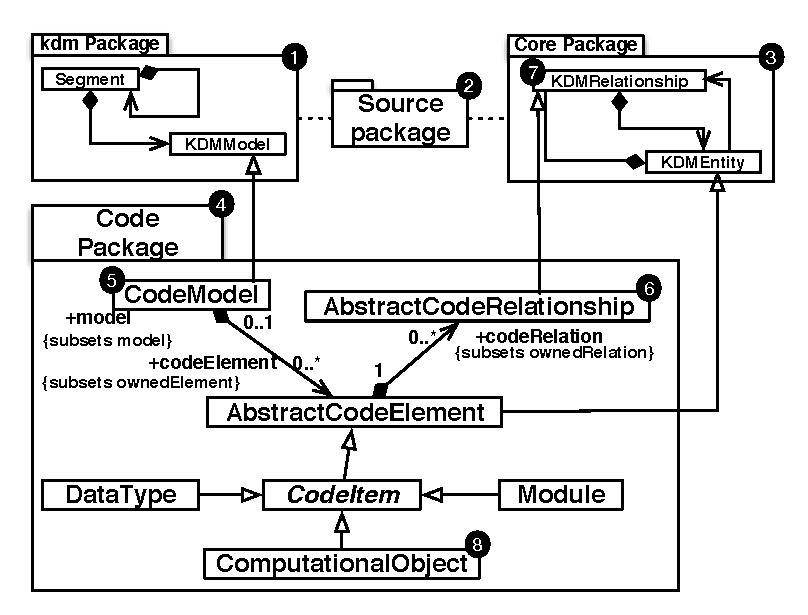
\includegraphics[scale=0.8]{images/codeModel}
	\caption{Diagrama de classes - $\mathtt{CodeModel}$}
	\label{fig:CodeModel}
	\fadaptada{KDM:specification}
\end{figure}

A metaclasse \texttt{CodeModel} representa um contêiner para outras instâncias de elementos do tipo~$\mathtt{Code}$. Como pode ser observado, o pacote $\mathtt{Code}$ \ding{205} depende dos outros pacotes $\mathtt{kdm}$ \ding{202}, $\mathtt{Source}$ \ding{203} e $\mathtt{Core}$ \ding{204}. A metaclasse $\mathtt{CodeModel}$ \ding{206} é um modelo que possui coleções de fatos sobre o sistema de software, correspondentes ao domínio $\mathtt{Code}$. Ela possui uma associação  $\mathtt{codeElement:AbstractCodeElement[0..*]}$ permitindo a adição de novos elementos de código, por exemplo, métodos, atributos, etc. A metaclasse  $\mathtt{AbstractCodeRelationship}$ \ding{207} representa qualquer relacionamento determinado por em uma linguagem de programação. Por sua vez, a metaclasse $\mathtt{ComputationalObject}$ representa os elementos determinados pela linguagem de programação, que descreve certos objetos computacionais em tempo de execução, por exemplo, métodos e variáveis.

%This metamodel element is a container for other \texttt{code} element instances. As can be observed in Figure~\ref{fig:CodeModel} the \texttt{Code} package \ding{205} depends on the \texttt{kdm} \ding{202}, \texttt{Source} \ding{203}, and \texttt{Core} \ding{204} packages. The meta-class \texttt{CodeModel} \ding{206} is the specific KDM model that owns collections of facts about the existing software system such that these facts correspond to the \texttt{Code} domain, its superclass is \texttt{KDMModel}. It has as association \texttt{codeElement:AbstractCodeElement[0..*]} meaning that one shall arrange code elements (e.g., methods, fields, etc) into one or more code models. The \texttt{AbstractCodeRelationship} \ding{207} is an abstract meta-class representing any relationship determined by a programming language, it is also used to constrain the subclasses of \texttt{KDMRelationship} (see Figure~\ref{fig:CodeModel} \ding{208}) in the \texttt{Code} model. The meta-class \texttt{ComputationalObject} represents the named elements determined by the programming language, which describe certain computational objects at the runtime, for example, methods, and variables.

O pacote~$\mathtt{Code}$ consiste em um total de 24 metaclasses; tais metaclasses são um arranjo de abstrações para representar toda, ou a grande maioria, da estrutura estática de um terminado código-fonte dado um linguagem de programação, seja ela procedural ou orientada a objetos~\cite{KDM:specification}. Na Tabela~\ref{tab:meta_classes_pacoteCODE} algumas metaclasses são apresentadas. Como pode ser observado algumas metaclasses podem ser diretamente elucidadas e mapeadas, como por exemplo, \aspas{classes} e \aspas{interfaces} construções facilmente encontradas em linguagens orientadas a objetos podem ser facilmente mapeada para as metaclasses denominada $\mathtt{ClassUnit}$ e $\mathtt{InterfaceUnit}$, respectivamente. Um mapeamento mais completo entre elementos estruturais e metaclasses do KDM pode ser identificado em~\citeonline{bruno_marinho_dissertacao}. Uma representação dessas metaclasses, bem como seus relacionamentos são apresentados em diagrama de classe na Figura~\ref{fig:classUnit_e_InterfaceUnit}. 

\begin{figure}[!ht]
	\centering
	% Requires \usepackage{graphicx}
	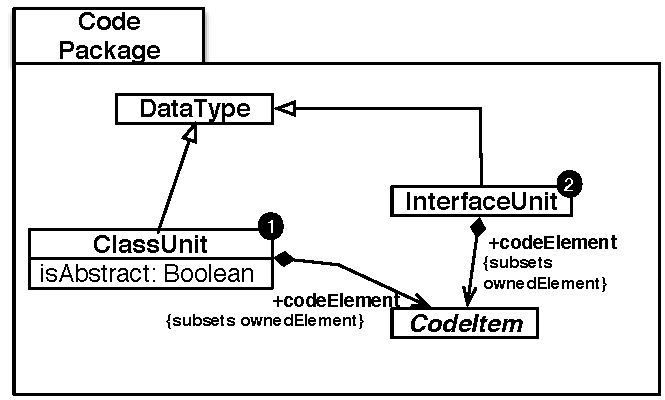
\includegraphics[scale=0.8]{images/ClassUnit_InterfaceUnit}
	\caption{Diagrama de classes elucidando as metaclasses \texttt{ClassUnit} e \texttt{InterfaceUnit}}
	\label{fig:classUnit_e_InterfaceUnit}
	\fadaptada{KDM:specification}
\end{figure}

%The whole \texttt{Code} package consists of $24$ metaclasses\footnote{Note that not all the meta-class are shown in Figure~\ref{fig:CodeModel}} and contains all the abstract elements for modeling the static structure of the source code. In Table~\ref{tab:mappingCodeToKDM} is depicted some of them. This table identifies KDM metaclasses possessing similar characteristics to the static structure of the source code. Some metaclasses can be direct mapped, such as class from object-oriented language, which can be easily mapped to the \texttt{ClassUnit} meta-class from KDM. For instance, the meta-class \texttt{Package} is a subtype for \texttt{Module} that logical collections of program elements, as directly supported by some programming languages, such as Java. 

\begin{table}[h]
\centering
\caption{metaclasses para modelagem de estruturas estáticas do código-fonte}
\label{tab:meta_classes_pacoteCODE}
\begin{tabular}{|l|l|}
\hline
Elemento do Código-Fonte & metaclasses do KDM \\ \hline
Classe                   & \texttt{ClassUnit}           \\ \hline
Interface                & \texttt{InterfaceUnit}       \\ \hline
Método                   & \texttt{MethodUnit}          \\ \hline
Atributo                 & \texttt{StorableUnit}        \\ \hline
Variável Local           & \texttt{MemberUnit}          \\ \hline
Parâmetro                & \texttt{ParameterUnit}       \\ \hline
Associação               & \texttt{KDMRelationShip}     \\ \hline
\end{tabular}
\end{table}

%\begin{table}[!h]
	%\caption{metaclasses para modelagem de estruturas estáticas do código fonte}
%	\label{tab:mappingCodeToKDM}
%	\centering
%	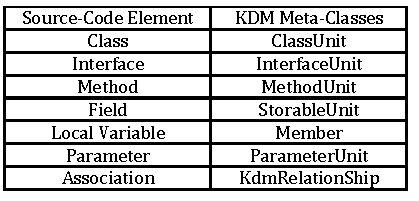
\includegraphics[scale=1]{images/tabela_comparativo_KDM_code_com_source_code}
%\end{table}

$\mathtt{ClassUnit}$ e $\mathtt{InterfaceUnit}$ representam \aspas{classes} e \aspas{interfaces} que são definidas por usuários de linguagens orientadas a objeto. Ambas metaclasses possuem caracteristicas e relacionamentos similares, como observado na Figura~\ref{fig:classUnit_e_InterfaceUnit} \ding{202} e \ding{203}. Uma das diferenças que pode ser destacada é que a metaclasse ~$\mathtt{ClassUnit}$ contém um meta-atributo~$\mathtt{isAbstract:Boolean}$, o qual é utilizado para especificar se uma classe é ou não abstrata. $\mathtt{ClassUnit}$ e $\mathtt{InterfaceUnit}$ podem conter um coleção de elementos que seja do tipo ~$\mathtt{CodeItem}$, por exemplo,~$\mathtt{StorableUnit}$ ou ~$\mathtt{MethodUnit}$. Além disso, tais metaclasses  possuem uma meta-associação denominada ~$\mathtt{codeElement:CodeItem[0..*]}$ que é utilizada para agrupar todos os membros da classe, por exemplo, construtores, métodos, atributos, etc. Na Figura~\ref{fig:StorableUnit_MethodUnit} é apresentado os meta-atributos e metarelacionamentos das metaclasses \texttt{StorableUnit} \ding{204}, \texttt{MethodUnit} \ding{205}, \texttt{ParameterUnit} \ding{207} e \texttt{MemberUnit} \ding{206}.

\begin{figure}[!ht]
	\centering
	% Requires \usepackage{graphicx}
	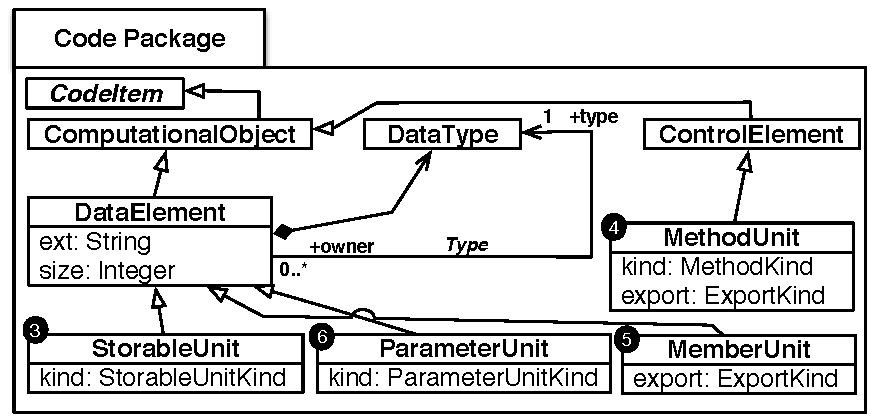
\includegraphics[scale=0.8]{images/StorableUnit_MethodUnit2}
	\caption{Diagrama de classes elucidando as metaclasses \texttt{StorableUnit}, \texttt{MethodUnit}, \texttt{ParameterUnit} e \texttt{MemberUnit}}
	\label{fig:StorableUnit_MethodUnit}
	\fadaptada{KDM:specification}
\end{figure}


%As stated before, the meta-class \texttt{ClassUnit} represents user-defined classes in object-oriented languages. A class datatype is a named datatype that represents a class: an ordered collection of named elements, each of which can be another \texttt{CodeItem}, such as a \texttt{StorableUnit} or a \texttt{MethodUnit}. The meta-class \texttt{ClassUnit} contains a meta-attribute \texttt{isAbstract:Boolean} used to specify if the class is abstract or not. \texttt{ClassUnit} also has an meta-association named \texttt{codeElement:CodeItem[0..*]} that is used to group all class's members, e.g., fields, constructor, methods, etc. 

%Similarmente, a metaclasse~$\mathtt{InterfaceUnit}$ representa o conceito comum a várias linguagens de programação. Ela é uma subclasse de~$\mathtt{DataType}$, assim como~$\mathtt{ClassUnit}$.~$\mathtt{InterfaceUnit}$ também possui uma meta associação chamada~$\mathtt{codeElement:CodeItem[0..*]}$ que representa tipos de dados tal como~$\mathtt{MethodUnit}$.

%Similarly, the meta-class \texttt{InterfaceUnit} represents the interface concept common to various programming languages. It is also a subclass of \texttt{Datatype} as \texttt{ClassUnit}. \texttt{InterfaceUnit} also has an meta-association named \texttt{codeElement:CodeItem[0..*]} that represent data types as well as \texttt{MethodUnits}.

$\mathtt{StorableUnit}$ representa um atributo em um sistema de software - um objeto computacional para que diferentes valores do mesmo tipo de dados possa ser associado em vezes diferentes. Ele é usado para representar as variáveis globais e locais. Ele contém uma meta atributo~$\mathtt{String}$ usado para definir o nome das variáveis.~$\mathtt{StorableUnit}$ também tem a associação~$\mathtt{type:DataType[1]}$, a qual é herdada da metaclasse~$\mathtt{DataElement}$, e é utilizado para especificar o tipo da variável (\textit{int, char, boolean, numeric}, etc). Ele também tem uma enumeração ~$\mathtt{kind:StorableUnit}$, que descreve várias propriedades comuns de um ~$\mathtt{StorableUnit}$ relacionado com o seu ciclo de vida, por exemplo, sua visibilidade (\textit{private, public, protected}, etc).

%\texttt{StorableUnit} represents a variable of existing software system - a computational object to which different values of the same datatype can be associated at different times. It is used to represent both global and local variables. It contains a meta-attribute \texttt{name:String} used to set the name of the variables. \texttt{StorableUnit} also has the association \texttt{type:Datatype[1]} used to specify the variable's type. It also has a enumeration \texttt{kind:StorableKind}, it describes several common properties of a \texttt{StorableUnit} related to their life-cycle, visibility, and memory type. 

~$\mathtt{MethodUnit}$ como o próprio nome sugere representa métodos que são identificados em ~$\mathtt{ClassUnit}$ ou~$\mathtt{InterfaceUnit}$. Ele também é usado para representar construtores e destrutores. Possui como meta-atributos~$\mathtt{name:String}$,~$\mathtt{kind:MethodKind}$ e ~$\mathtt{export:ExportKind}$. O primeiro é usado para descrever o nome de um método. O segundo meta-atributo é uma enumeração que define especificações adicionais do tipo de método, ou seja, é possível especificar se a instância do método é um construtor, destrutor, ou um método normal. O último representa a visibilidade do método (\textit{private, public, protected}, etc).

%\texttt{MethodUnit} represents member functions owned by either \texttt{ClassUnit} or \texttt{InterfaceUnit}. It is also used to represent user-defined operators, constructors, and destructors. It owns as meta-attributes \texttt{name:String}, \texttt{kind:MethodKind}, and \texttt{export: ExportKind}. The fist one is used to describe to name of a method. The second meta-attribute is an enumeration that defines additional specification of the kind of method, i.e., it is possible to specify if the method's instance is a constructor, destructor, abstract, etc. The last one represents the visibility of the method, i.e., \texttt{public}, \texttt{private}, \texttt{protected}.

A fim de entender como o KDM é utilizado para representar estruturas um determinado programa, no Código-fonte~\ref{lst:example_kdm_instance} é mostrado um exemplo simplificado escrito em Java. O correspondente KDM, embora simplificado, é apresentado na Figura~\ref{fig:kdm_instance_Java}. Por questões de simplicidade e para facilitar o entendimento, essa figura ilustra a instância do KDM em forma de um diagrama de objetos; é possível notar que este diagrama representa o código-fonte como uma árvore, na qual cada nó representa uma metaclasses do KDM. Como pode ser visto na Figura~\ref{fig:kdm_instance_Java}, a metaclasse raiz é ~$\mathtt{Segment}$, que é um recipiente para um conjunto significativo de fatos sobre um sistema de software existente. Cada~$\mathtt{Segment}$ pode incluir uma ou mais instâncias de modelos do KDM, como~$\mathtt{CodeModel}$ e~$\mathtt{StructureModel}$.

%In order to fully understand how KDM is used to represent the source code of a specific program, in Listing~\ref{lst:example_kdm_instance} is shown a simplified example in Java. The corresponding, though simplified KDM instance is depicted in Figure~\ref{fig:kdm_instance_Java}. It illustrates a KDM instance as a UML object diagram for the sake of simplicity, note that this diagram represents the source code as a tree of nodes containing some KDM's metaclasses. As can be seen in Figure~\ref{fig:kdm_instance_Java} the root meta-class is \texttt{Segment}, which is a container for a meaningful set of facts about an existing software system. Each \texttt{Segment} may include one or more KDM model instances, such as \texttt{CodeModel} and \texttt{StructureModel}. As stated earlier, the \texttt{CodeModel} is the specific KDM container for other \texttt{code} element instances (see Figure~\ref{fig:CodeModel}). 

Analisando tanto o Código-fonte~\ref{lst:example_kdm_instance} quanto a Figura~\ref{fig:kdm_instance_Java} é evidente que cada estrutura estática do código-fonte tem uma metaclasse específica em KDM para representá-la. Por exemplo, a declaração \textit{package} \textit{model} na Linha 1 do Código-fonte~\ref{lst:example_kdm_instance} \ding{202} é representada em KDM pela metaclasse ~$\mathtt{package}$, como visto na Figura~\ref{fig:kdm_instance_Java} \ding{202}. Posteriormente, como apresentado no Código-fonte~\ref{lst:example_kdm_instance} \ding {203} uma classe~$\mathtt{Car}$ é declarada. Essa classe herda caracteristicas da classe~$\mathtt{Vehicle}$, no Java isso é feito por meio da palavra-chave~$\mathtt{extends}$ seguido do nome de uma classe, conforme por ser observado no Código-fonte~\ref{lst:example_kdm_instance} \ding{204} e \ding{205}. A metaclasse~$\mathtt{Extends}$ representa o conceito de herança em KDM. Como mostrado na Figura~\ref{fig:kdm_instance_Java} \ding {204} a metaclasse~$\mathtt{Extends}$ possui duas associações,~$\mathtt{to}$ e~$\mathtt{from}$, o primeiro representa a classe pai (\textit{super class}), e o último a classe filha(\textit{sub-class}). Neste contexto, a classe~$\mathtt{Car}$ e classe pai de~$\mathtt{Vehicle}$, como mostrado na Figura~\ref{fig:kdm_instance_Java} \ding{205}. Finalmente, o atributo~$\mathtt{name}$ e o método~$\mathtt{getName()}$ (ver Código-fonte~\ref{lst:example_kdm_instance} \ding {206} e \ding {207}, respectivamente) são mapeados para os correspondentes elementos do KDM,~$\mathtt{StorableUnit}$ e~$\mathtt{MethodUnit}$ (ver Figura ~\ref{fig:kdm_instance_Java} \ding {206} e \ding {207}).

%Analyzing both the Listing~\ref{lst:example_kdm_instance} and the Figure~\ref{fig:kdm_instance_Java} it is evident that each static structure of the source code has a meta-class in KDM to represent it. For instance, the package model in Line 1 of Listing~\ref{lst:example_kdm_instance} \ding{202} is represented in KDM by the meta-class named \texttt{Package}, see Figure~\ref{fig:kdm_instance_Java} \ding{202}. In addition, the class \texttt{Car} is declared, see Listing~\ref{lst:example_kdm_instance} \ding{203}. It also inherit from class \texttt{Vehicle}, in the Java this is accomplished by using the keyword \texttt{extends} following of a class, see Listing~\ref{lst:example_kdm_instance}  \ding{204} and \ding{205}. The meta-class \texttt{Extends} represents inheritance in KDM models. As shown in Figure~\ref{fig:kdm_instance_Java} \ding{204} the meta-class \texttt{Extends} has two association, \texttt{to} and \texttt{from}, the former represents the parent class (super class), and the latter represents the child class (sub-class). In this context, the child is the class \texttt{Car} and the parent class is \texttt{Vehicle}, which is depicted in Figure~\ref{fig:kdm_instance_Java} \ding{205}. Finally, the variable \texttt{name}, and the method \texttt{getName()} (see Listing~\ref{lst:example_kdm_instance} \ding{206}, and \ding{207}) are mapped to corresponding instances of the KDM elements, \texttt{StorableUnit}, and \texttt{MethodUnit} (see Figure~\ref{fig:kdm_instance_Java} \ding{206}, and \ding{207}). 


\noindent\begin{minipage}{.53\textwidth}
	\begin{codigo}[caption={[Parte de código Java para ilustrar como o KDM é usado para representar o código fonte.] Simples código em java.},escapeinside={(*@}{@*)}, basicstyle=\footnotesize, label={lst:example_kdm_instance}]{Name}
	(*@\ding{202}@*) package model;
	(*@\ding{203}@*) public class Car (*@\ding{204}@*) extends  
	(*@\ding{205}@*) Vehicle{
	(*@\ding{229}@*)(*@\ding{206}@*) private String name;
	(*@\ding{229}@*)(*@\ding{207}@*) public String getName(){
	(*@\ldots @*)
	}
	}
	\end{codigo}
\end{minipage}\hfill
\begin{minipage}{.45\textwidth}
	\centering
	% Requires \usepackage{graphicx}
	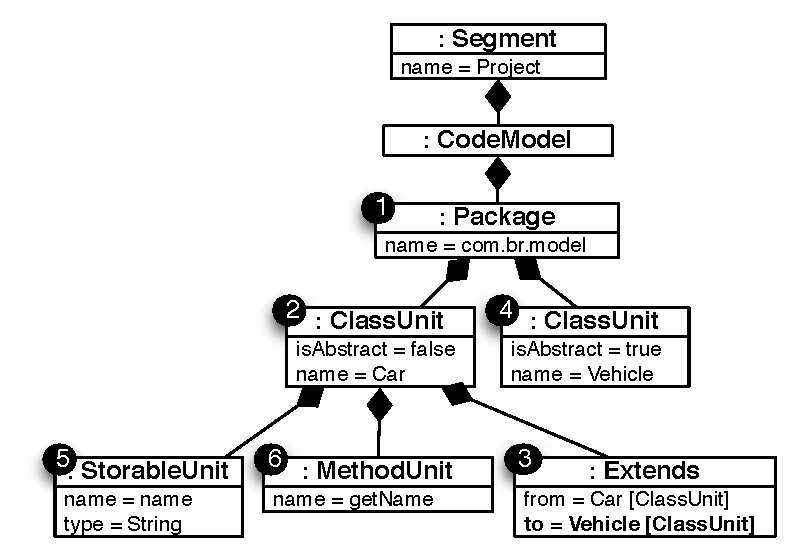
\includegraphics[scale=0.6]{images/kdm_instance_java_correspoding_2_with_extends}
	\captionof{figure}{Instância KDM correspondente ao Código-fonte~\ref{lst:example_kdm_instance}}
	\label{fig:kdm_instance_Java}
\end{minipage}


Apenas metaclasses utilizadas para representar estruturas e construções estáticas foram apresentadas. No entanto, o KDM contêm um pacote que permite a representação de construções dinâmicas, em outras palavras, o pacote \textit{Action} contêm metaclasses cuja finalidade é permitir e representar comportamento em nível de execução. Na seção a seguir mais informações sobre esse pacote é apresentado.

\subsection{Pacote Action}\label{sec:actionPackage}

O pacote~$\mathtt{Action}$ define um conjunto de metaclasses, cujo propósito é o de representar descrições de comportamento em nível de implementação estabelecido por linguagens de programação, por exemplo, declarações, operadores, condições e as suas associações. A Figura ~\ref{fig:actionModel} \ding {202} mostra o pacote~$\mathtt{Action}$ e algumas de suas metaclasses. Como pode ser observado, este pacote estende o pacote~$\mathtt{Code}$ (ver a Figura~\ref {fig:actionModel} \ding {208}).

%The \texttt{Action} package defines a set of metaclasses whose purpose is to represent implementation-level behavior descriptions determined by programming languages, for example statements, operators, conditions, features, as well as their associations, for example control and data flow. The Figure~\ref{fig:actionModel} \ding{202} shows the\texttt{Action} package and some of its metaclasses. As can be observed it extends the KDM \texttt{Code} package (see Figure~\ref{fig:actionModel} \ding{208}). 

\begin{figure}[!ht]
	\centering
	% Requires \usepackage{graphicx}
	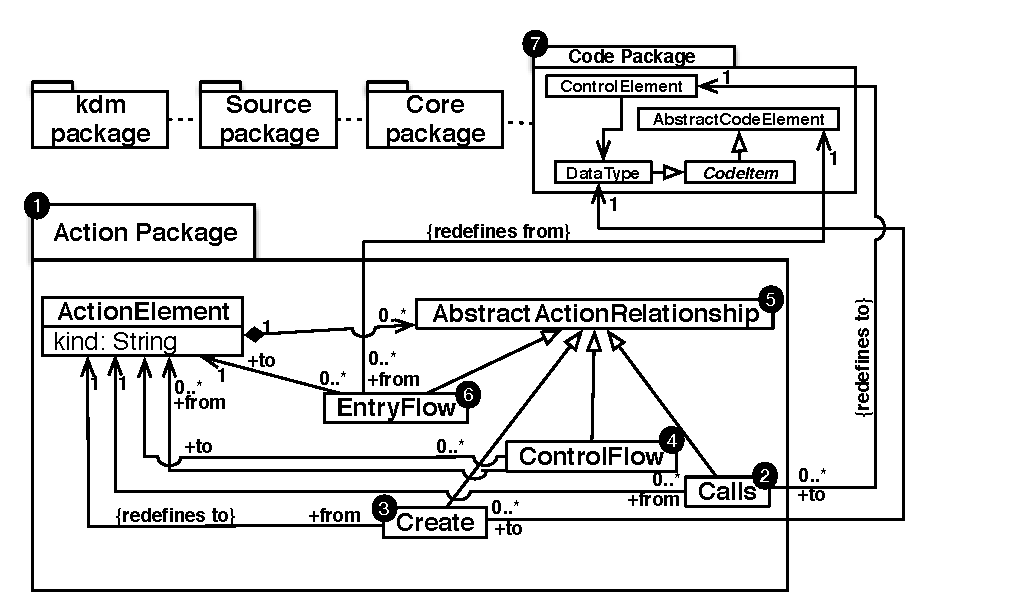
\includegraphics[scale=0.8]{images/ActionModel_Class_Diagram}
	\caption{Diagrama de classes ilustrando o pacote~$\mathtt{Action}$.}
	\label{fig:actionModel}
	\fadaptada{KDM:specification}
\end{figure}

O pacote~$\mathtt{Action}$ é composto por 11 diagramas de classe, ele também depende dos pacotes~$\mathtt{Core}$, ~$\mathtt{kdm}$ e ~$\mathtt{Source}$, e  principalmente do pacote~$\mathtt{Code}$. No entanto, o pacote~$\mathtt{Action}$ segue o padrão uniforme para os modelos KDM e estende o KDM com metaclasses específicas relacionadas com o comportamento do nível de implementação. O pacote~$\mathtt{Action}$ se desvia de um padrão uniforme para os modelos KDM porque ele não define um modelo KDM separado, mas estende o pacote~$\mathtt{Code}$.  Por isso, cada metaclasse do pacote ~$\mathtt{Action}$ é uma subclasse de~$\mathtt{AbstractCodeElement}$, conforme destacado na Figura~\ref{fig:actionModel}. O pacote~$\mathtt{Action}$ define a maioria das metaclasses que tem como objetivo representar comportamentos para as construções estáticas definidas no pacote~$\mathtt{Code}$. Assim, ambos pacotes constituem a CEP, como mostrado na Figura~\ref{fig:kdm_layer}.

%The \texttt{Action} package consists of 11 class diagrams, it also depends on the \texttt{Core}, \texttt{kdm}, \texttt{Source}, and mainly \texttt{Code}. However, the \texttt{Action} package follows the uniform pattern for KDM models and extends the KDM with specific metaclasses related to implementation-level behavior. The \texttt{Action} package deviates from a uniform pattern for KDM models because it does not define a separate KDM model, but rather extends the \texttt{Code}, which is presented in Section~\ref{codePackage}. Therefore each \texttt{Action} metaclasses is a subclass of \texttt{AbstractCodeElement}, as highlighted in Figure~\ref{fig:actionModel}. \texttt{Action} package defines most of the relationship types to the \texttt{Code} model. Together, \texttt{Action}, and \texttt{Code} packages constitute the Program Elements Layer of KDM as depicted in Figure~\ref{fig:all_kdm_layers}. 

A metaclasse~$\mathtt{AbstractionActionRelationship}$ apresentada na Figura~\ref{fig:actionModel} \ding{206} é a metaclasse pai usada para representar várias relações que se originam a partir de um~$\mathtt{ActionElement}$. Além disso, essa metaclasse~$\mathtt{AbstractionActionRelationship}$ possui metaclasses específicas; algumas delas estão representadas na Figura~\ref{fig:actionModel}, por exemplo, as metaclasses~$\mathtt{Calls}$ \ding {203},~$\mathtt{Creates}$ \ding {204},~$\mathtt{ControlFlow}$ \ding {205} e~$\mathtt{EntryFlow}$ \ding{207}.

%The meta-class \texttt{AbstractActionRelationship} presented in Figure~\ref{fig:actionModel} \ding{206} is the parent class used to represent various KDM relationships that originate from an \texttt{ActionElement}. The meta-class \texttt{AbstractActionRelationship} owns specific metaclasses. Some of them are depicted in Figure~\ref{fig:actionModel}, for example, the metaclasses \texttt{Calls} \ding{203}, \texttt{Create} \ding{204}, \texttt{ControlFlow} \ding{205}, and \texttt{EntryFlow} \ding{207}.

O relacionamento~$\mathtt{Calls}$ corresponde a uma chamada para um procedimento, um método estático, um método não-estático de uma instância particular de um objeto, um método virtual, ou um elemento de interface.~$\mathtt{Calls}$ possui duas associações, são elas: ~$\mathtt{ActionElement[1]}$ e ~$\mathtt{ControlElement[1]}$. O primeiro representa o elemento de ação a partir do qual a relação chamada origina, a segunda associação representa o elemento alvo.

%\texttt{Calls} relationship corresponds to ``invoke'' operation on a procedure type. It can represent a call to a procedure, a static method, a non-static method of a particular object instance, a virtual method, or an interface element. \texttt{Calls} has two associations, they are: \texttt{from:ActionElement[1]} and \texttt{to:ControlElement[1]}. The first one represents the action element from which the call relation originates. The second association represents the target \texttt{ControlElement}.

A metaclasse~$\mathtt{Creates}$ representa uma associação entre um elemento de ação que \aspas{cria} uma nova instância de um determinado elemento de dados. Por exemplo, em Java essa metaclasse corresponde a palavra-chave \textit{new} utilizada para instânciar um novo objeto. $\mathtt{Creates}$ também possui duas associações:~$\mathtt{ActionElement[1]}$ e~$\mathtt{DataType[1]}$. Similar a metaclasse~$\mathtt{Calls}$, a primeira associação representa o elemento que possui o relacionamento e a segunda representa o elemento de dados (objeto) que é instanciado pelo~$\mathtt{ActionElement}$.

%The meta-class \texttt{Create} represents an association between an action element that ``creates'' a new instance of a certain data element to the corresponding datatype according to the semantics of the programming language of the existing software system. It also has association, \texttt{from:ActionElement[1]} and \texttt{to:Datatype[1]}. Similarly, to the meta-class \texttt{Calls}, the first association represents the element that owns the \texttt{Creates} relationship. The second one illustrates the \texttt{DataElement} that is instantiated by the \texttt{ActionElement}. 

O~$\mathtt{ControlFlow}$ é um elemento de modelagem genérica que representa relação de fluxo de controle entre dois~$\mathtt{ActionElements}$. Além disso, é uma submetaclasse com elementos de modelagem mais específicas. O~$\mathtt{EntryFlow}$ é um elemento de modelagem que representa um fluxo inicial de controle em um elemento KDM. O relacionamento~$\mathtt{EntryFlow}$ é usado de uma maneira uniforme para descrever os pontos de entrada para outros elementos de código KDM.

%The \texttt{ControlFlow} is a generic modeling element that represents control flow relation between two \texttt{ActionElements}. It is further subclassed with more specific modeling elements. The \texttt{EntryFlow} is a modeling element that represents an initial flow of control into a KDM element. The \texttt{EntryFlow} relationship is used in a uniform way for describing entry points to other KDM code elements. 

A fim de compreender como o pacote~$\mathtt{Action}$ é usado no KDM, no Código-fonte~\ref{lst:example_kdm_instance_2} é mostrado um simples método implementado em Java. Neste método é criada uma instância de~$\mathtt{Car}$ e seu método de acesso é invocado. Uma possível correspondente instância do KDM simplificada é apresentada na Figura~\ref{fig:kdm_instance_Java_action}. Nota-se que, o diamante em destaque na cor cinza e anexado com três pontos (\ldots) ilustra que outras metaclasses não são mostrados com o intuito de simplificar a figura.

%In order to comprehend  how the \texttt{Action} package is used in KDM, in Listing~\ref{lst:example_kdm_instance_2} shows a simple method implemented in Java. In this method is created an instance of \texttt{Car} and an accessor method of it is called, ie., the \texttt{getName()}. The corresponding simplified KDM instance is depicted in Figure~\ref{fig:kdm_instance_Java_action}. Please note that, the diamond highlighted in grey and attached with three dots (\ldots) illustrates that other metaclasses are not shown in order to simplify the figure.  

\noindent\begin{minipage}{.43\textwidth}
	\begin{codigo}[caption={[Pedaço de código Java para ilustrar como o pacote~$\mathtt{Action}$ funciona.] Método \texttt{e1} ilustrando como o Pacote \texttt{Action} funciona.}, escapeinside={(*@}{@*)}, basicstyle=\footnotesize, label={lst:example_kdm_instance_2}]{Name}
	(*@\ldots @*)
	public void e1 (*@\ding{202}@*)(){
	Car myCar (*@\ding{203}@*) = new Car() (*@\ding{204}@*);
	(*@\ding{229}@*)myCar.getName() (*@\ding{205}@*);
	}
	(*@\ldots @*)
	\end{codigo}
\end{minipage}\hfill
\begin{minipage}{.65\textwidth}
	\centering
	% Requires \usepackage{graphicx}
	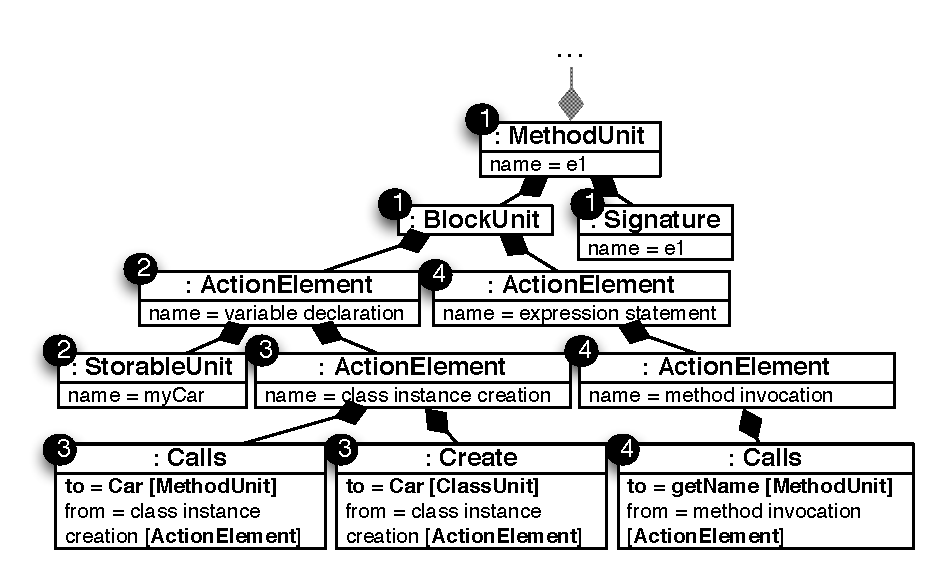
\includegraphics[scale=0.6]{images/actionInstanceKDM_2}
	\captionof{figure}{Instância KDM correspondente ao Código-fonte~\ref{lst:example_kdm_instance_2}}
	\label{fig:kdm_instance_Java_action}
\end{minipage}

As três primeiras metaclasses mostradas nesta hierarquia são~$\mathtt{MethodUnit}$,~$\mathtt{BlockUnit}$ e~$\mathtt{Signature}$ conforme destacado na  Figura~\ref{fig:kdm_instance_Java_action} \ding{202}. Essas três metaclasses basicamente representam uma declaração e a assinatura de um determinado método, no caso \texttt{e1()}. Mais especificamente, a metaclasse~$\mathtt{MethodUnit}$ é usada para representar o método~$\mathtt{e1()}$ como mostrado tanto no Código-fonte~\ref{lst:example_kdm_instance_2} \ding{202} e na Figura~\ref{fig:kdm_instance_Java_action} \ding{202}.~$\mathtt{BlockUnit}$ representa blocos lógicos e físicos relacionados de~$\mathtt{ActionElement}$, ou seja, o escopo do método representado por \{...\}. Por sua vez,~$\mathtt{Signature}$ representa a assinatura do método, isto é, essa metaclasse representa além do nome do método todos os parâmetros, o retorno do método, exceções, etc.	

%The first three metaclasses shown in this hierarchy are the \texttt{MethodUnit}, \texttt{BlockUnit}, and \texttt{Signature} (see Figure~\ref{fig:kdm_instance_Java_action} \ding{202}). These metaclasses are used to represent a simple method declaration. More specifically, the meta-class \texttt{MethodUnit} is used to represent the method \texttt{e1} as shown in both Listing~\ref{lst:example_kdm_instance_2} \ding{202} and Figure~\ref{fig:kdm_instance_Java_action} \ding{202}. \texttt{BlockUnit} represents logically and physically related blocks of \texttt{ActionElement}, i.e., the area between the braces, \texttt{\{\ldots\}}. In turn, \texttt{Signature} represents the concept of a method signature, i.e., it also can be used to represent the name of the method, all the parameters, the return of the method, etc.

Na Linha 12 do Código-fonte~\ref{lst:example_kdm_instance_2} \ding{203} uma variável chamada~$\mathtt{myCar}$ é declarada. As metaclasses que representam esta declaração podem ser visualizadas na Figura~\ref{fig:kdm_instance_Java_action} \ding{203}. A metaclasse~$\mathtt{ActionElement}$ representa o significado das operações, por exemplo, um declaração da variável. A metaclasse~$\mathtt{StorableUnit}$ representa a própria variável, \texttt{myCar}. Ainda na Linha 10 \ding{204} a instância da classe~$\mathtt{Car}$ é criada usando a palavra-chave~$\mathtt{new}$. Nota-se que na Figura~\ref{fig:kdm_instance_Java_action} \ding{204} três metaclasses são utilizadas para representar o operador~$\mathtt{new}$. Primeiramente, a metaclasse~$\mathtt{ActionElement}$ é usada para ilustrar o significado da operação, neste caso, a instância da classe \texttt{Car}. A metaclasse~$\mathtt{Calls}$ é usada para ilustrar a instanciação de um objeto, neste caso, o objeto~$\mathtt{Car}$. Adicionalmente, a metaclasse \texttt{Calls} posssui duas ~$\mathtt{to}$ e~$\mathtt{from}$, as quais representam a chamada para o construtor de~$\mathtt{Car}$ e representa o alvo~$\mathtt{ActionElement}$, respectivamente. Em seguida, a metaclasse~$\mathtt{Creates}$ representa a nova instância de~$\mathtt{Car}$.

%In Line 10 of the Listening~\ref{lst:example_kdm_instance_2} \ding{203} a variable named \texttt{myCar} is declared. The corresponding metaclasses representing this variable declaration can be visualized in Figure~\ref{fig:kdm_instance_Java_action} \ding{203}. The meta-class \texttt{ActionElement} represents the meaning of the operations, i.e., ``variable declaration''. The \texttt{StorableUnit} represents the variable itself. Still in Line 10 \ding{204} the instance of the class \texttt{Car} is created by using the keyword \texttt{new}. Note that in Figure~\ref{fig:kdm_instance_Java_action} \ding{204} three metaclasses are used to illustrate the operator \texttt{new}. Firstly, the meta-class \texttt{ActionElement} is used to illustrate the meaning of the operation, in this case ``class instance creation'' . Secondly, the meta-class \texttt{Calls} is used to illustrate the instantiation of an object, herein \texttt{Car} object. Its owns two association, i.e., \texttt{to} and \texttt{from} which illustrates the call to the constructor of \texttt{Car} and represents the target \texttt{ActionElement}, respectively. Thirdly, the meta-class \texttt{Creates} represents the new instance of the \texttt{Car}.

Na linha 11 do Código-fonte~\ref{lst:example_kdm_instance_2} \ding{205} um método acessor é invocado. Como pode ser visto na Figura~\ref{fig:kdm_instance_Java_action} \ding{205}, três metaclasses são utilizadas no KDM para representar esta linha. Em primeiro lugar, é criado uma metaclasse~$\mathtt{ActionElement}$ que representa a declaração em si. Em seguida, outro~$\mathtt{ActionElement}$ é criado para representar a invocação de método. Finalmente, outra metaclasse~$\mathtt{Calls}$ é instânciada para representar a chamada do método~$\mathtt{getName()}$.


\subsection{Pacote \textit{Structure}}\label{sec:structurePackage}

O KDM define metaclasses que representam componentes arquiteturais, como subsistemas, camadas, componentes, etc., e define também a rastreabilidade desses elementos para outras metaclasses do KDM para o mesmo sistema por meio do pacote \texttt{Structure}.

\begin{figure}[h]
	\centering
	% Requires \usepackage{graphicx}
	\caption{Diagrama de classes do pacote \texttt{Structure}\label{fig:structureModel}}
	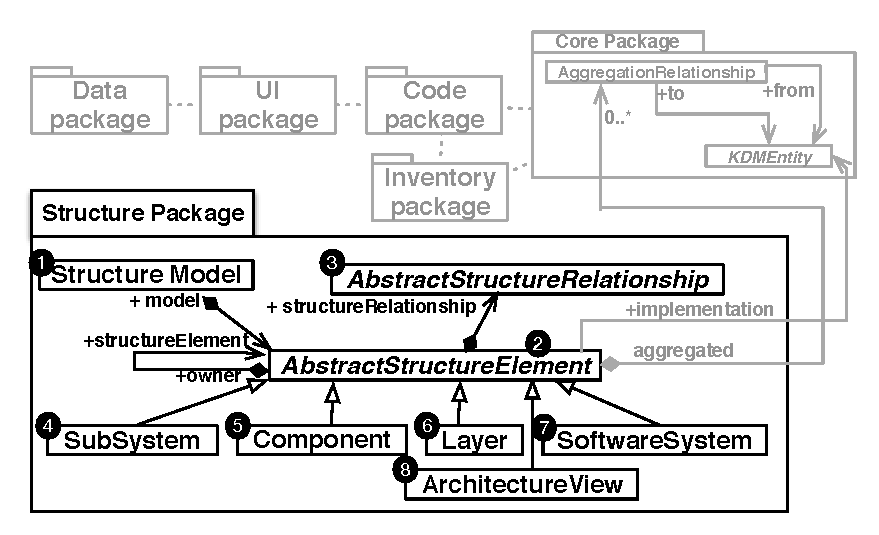
\includegraphics[scale=0.7]{images/StructurePackageFigure}
	\fadaptada{ADM:OMG}
\end{figure}

Esse pacote define um ponto de vista arquitetural para um domínio estrutural. As visões de arquitetura com bae no ponto de vista definido pelo pacote \texttt{Strcuture} representam a forma como os elementos estruturais do sistema de software estão relacionados como os módulos definidos em código-fonte, que correspondem ao pacote \texttt{Code} do KDM. Uma parte simplória do pacote \texttt{Structure} é apresentada na Figura~\ref{fig:structureModel} como um diagrama de classes.

 Usando suas metaclasses é possível relacionar todos os elementos estruturais do sistema, juntamente com os elementos computacionais, isto é, pode-se especificar os elementos estruturais do sistema. Na Figura~\ref{fig:structureModel} é mostrado que o pacote \texttt{Structure} e suas metaclasses são usadas em combinação com os pacotes \texttt{Code}, \texttt{Data}, \texttt{Platform}, \texttt{UI} e \texttt{Inventory}. O modelo \texttt{Structure} possui uma coleção de elementos estruturais, como pode ser visto na Figura~\ref{fig:structureModel} \ding{202}, isso é representado por meio de uma associação. Pacotes (do modelo \texttt{Code}) são os elementos folha do modelo \texttt{Structure}, representando a divisão de um sistema em módulos \texttt{Code} discretos, com partes não sobrepostas. A metaclasse \texttt{SoftwareSystem} fornece um ponto de encontro para todos os pacotes do sistema direta ou indiretamente através de outra associação chamada de \texttt{AbstractStructureElement[0..*]}. Os pacotes podem ainda ser agrupados nas metaclasses \texttt{SubSystem},\texttt{Layer},\texttt{Component} e \texttt{ArchitectureView}. 
 
A metaclasse \texttt{AbstractStructureElement} (conforme a Figura~\ref{fig:structureModel} \ding {203}) representa uma parte arquitetural, relacionada com a organização do sistema de software existente em módulos e possui quatro associações. A primeira associação representa os elementos pertencentes ao modelo e é chamada de $\mathtt{structureElement}$ $\mathtt{:AbstractStructureElement[0..*]}$. Em seguida, há a associação~$\mathtt{structureRelationship}$ $\mathtt{:AbstractStructureRelationship[0..*]}$, ela é usada para representar todas os relacionamentos em nível arquitetural. A associação $\mathtt{aggregated:}$ $\mathtt{AggregatedRelationship[0..*]}$ representa uma relação abstrata entre dois elementos do KDM, dentro dela é possível definir relações concretas. A última associação da metaclasse~$\mathtt{AbstractStructureElement}$ é o~$\mathtt{implementation:KDMEntity[0..*]}$. Esta associação é usada para especificar os elementos computacionais (do pacote~$\mathtt{Code}$, ou seja, $\mathtt{Package}$, $\mathtt{ClassUnit}$, $\mathtt{InterfaceUnit}$, etc) que representam o elemento estrutural. 

Na Figura~\ref{fig:kdm_structureExample} é descrita uma possível arquitetura mostrada para ilustrar como o KDM pode ser utilizado para representar elementos arquiteturais. Pode ser observado que esta figura é dividida em três níveis para ilustrar como o pacote~$\mathtt{Structure}$ está relacionado com o pacote~$\mathtt{Code}$. O nível mais baixo representa o código-fonte, artefatos físicos. L1 e L2 representam pacotes em código-fonte - cada caixa dentro dos pacotes representa as suas classes e interfaces, também é possível perceber que essas classes e interfaces são relacionados uns com os outros de alguma maneira. No meio há metaclasses do pacote~$\mathtt{Code}$, o que significa que as instâncias dessas meta -classes são usadas para representar os artefatos de baixo nível, ou seja, instâncias de~$\mathtt{Package}$ são usadas para representar L1 e L2 e instâncias de~$\mathtt{ClassUnit}$ e~$\mathtt{InterfaceUnit}$ são usados para representar as classes e interfaces, respectivamente. Finalmente, no nível superior a arquitetura é mostrada. Todos os elementos arquiteturais são representados com a seguinte padronização: a metaclasse que representa o elemento arquiteturais, ':' seguido pelo seu nome. A arquitetura apresentada é dividida da seguinte forma: no ponto mais alto de abstração há um~$\mathtt{SoftwareSystem}$ (~$\mathtt{S1}$) \ding {202}, que é dividido em duas camadas, ~$\mathtt{Layer}$~$\mathtt{L1}$ \ding {203} e ~$\mathtt{Layer}$~$\mathtt{L2}$ \ding {204}. Tais camadas representam elementos arquiteturais correspondentes aos pacotes L1 e L2 representadas no nível mais baixo. A~$\mathtt{Layer}$~$\mathtt{L1}$ pode acessar os elementos da~$\mathtt{Layer}$~$\mathtt{L2}$, essa restrição \aspas{pode acessar} é representada pela metaclasse~$\mathtt{AggregatedRelationship}$ \ding {205}. Além disso, a~$\mathtt{Layer}$~$\mathtt{L2}$ contém dois componentes,~$\mathtt{C1}$ \ding {206} e~$\mathtt{C2}$ \ding {207}. Finalmente, o~$\mathtt{Component}$~$\mathtt{C1}$ fornece recursos através de uma interface para o~$\mathtt{Component}$~$\mathtt{C2}$.

\noindent \begin{minipage}{.47\textwidth}
	\centering
	% Requires \usepackage{graphicx}
	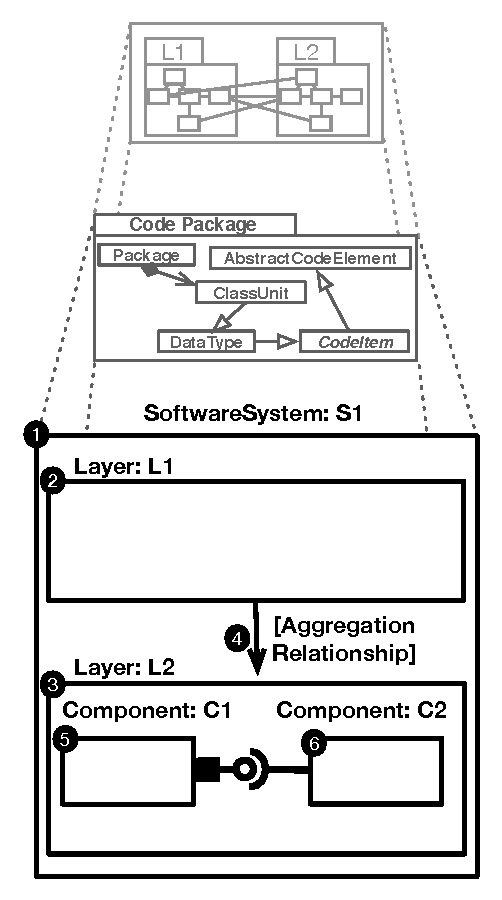
\includegraphics[scale=0.7]{images/StructureExample}
	\captionof{figure}{Exemplo de uma Arquitetura.}
	\label{fig:kdm_structureExample}
\end{minipage}\hfill
\begin{minipage}{.55\textwidth}
	\centering
	% Requires \usepackage{graphicx}
	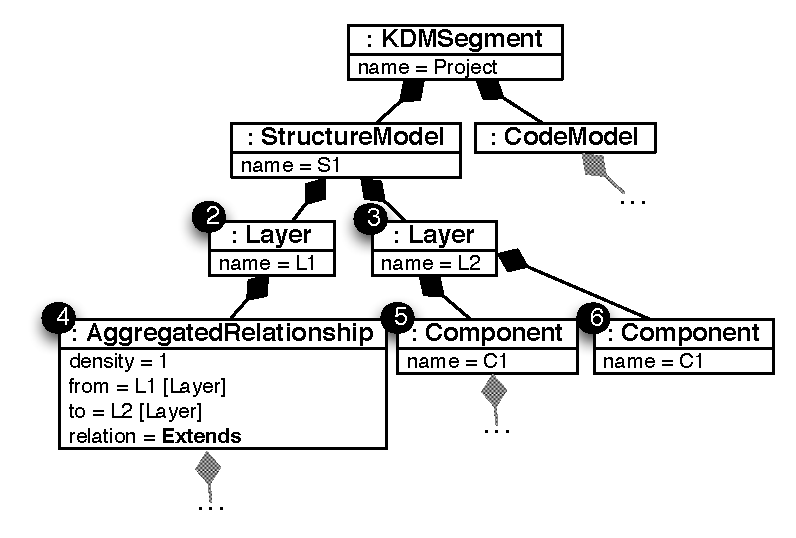
\includegraphics[scale=0.67]{images/StructureKDMINstance}
	\captionof{figure}{Instância KDM correspondente a Figura~\ref{fig:kdm_structureExample}}
	\label{fig:kdm_instance_StructureExample}
\end{minipage}


O correspondente, porém simplificado da instância KDM é mostrado na Figura~\ref{fig:kdm_instance_StructureExample}. Os diamantes destacadas em cinza e em anexo com três pontos (\ldots) ilustram que algumas metaclasses não são mostrados de forma a simplificar a figura. Todos os elementos arquiteturais são subclasses de~$\mathtt{StructureModel}$. As camadas são representados pela metaclasse~$\mathtt{Layer}$, como pode ser visto na Figura~\ref{fig:kdm_instance_StructureExample} \ding{203} e \ding{204}. Da mesma forma, os componentes são representados pela metaclasse~$\mathtt{Component}$. A metaclasse mais importante a se destacar nesta figura é $\mathtt{AggregatedRelationship}$. Ela representa a relação entre a $\mathtt{Layer}$ $\mathtt{L1}$ e a $\mathtt{Layer}$ $\mathtt{L2}$. Ela possui meta atributos que tem como objetivo fornecer informações sobre o relacionamento. Por exemplo, o meta atributo~$\mathtt{density}$ ilustra o número de relações primitivas entre estas camadas. Na Figura~\ref{fig:kdm_instance_StructureExample}, o meta atributo~$\mathtt{density}$ possui o valor 1 (um). Outros dois meta atributos são o~$\mathtt{from}$ e o~$\mathtt{to}$, que representam os elementos arquiteturais de origem e destino, respectivamente. Eles são usados para especificar que a~$\mathtt{Layer}$~$\mathtt{L1}$ em~$\mathtt{SoftwareSystem}$~$\mathtt{S1}$ pode acessar a~$\mathtt{Layer}$~$\mathtt{L2}$ também em~$\mathtt{SoftwareSystem}$~$\mathtt{S1}$ de alguma forma. Finalmente, o meta atributo~$\mathtt{relation}$ representa como a~$\mathtt{Layer}$~$\mathtt{L1}$ pode acessar a~$\mathtt{Layer}$~$\mathtt{L2}$, neste contexto, através de herança usando a metaclasse~$\mathtt{Extends}$. Na Figura~\ref{fig:relationship_example_1} é mostrado como as relações entre dois elementos arquiteturais são considerados neste estudo.

\begin{figure}[!ht]
	\centering
	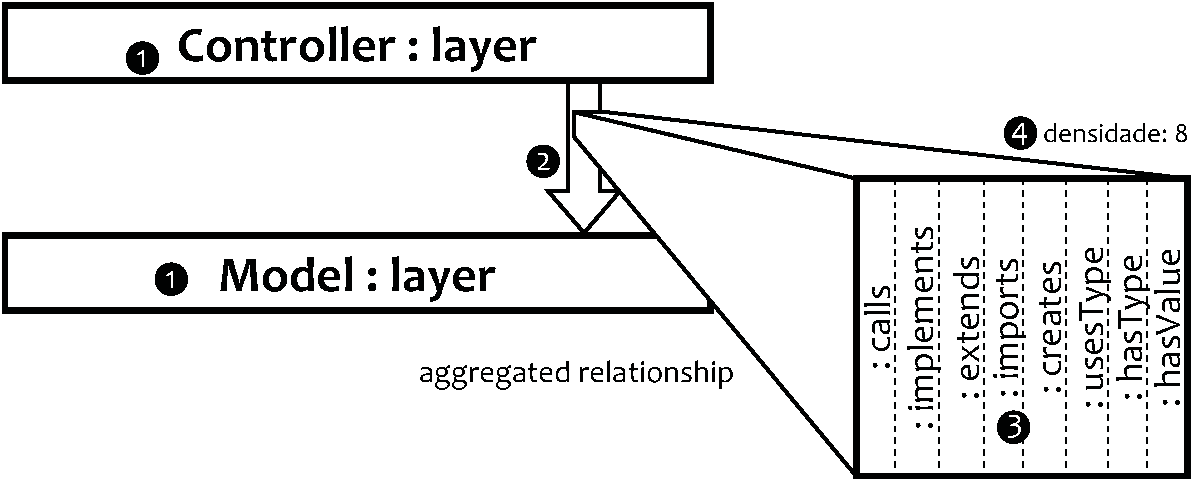
\includegraphics[width=3.3in]{images/relationshipExample1.pdf}
	\caption{Relacionamento entre dois elementos arquiteturais}
	\label{fig:relationship_example_1}
\end{figure}


Em \ding{202} os elementos arquiteturais são apresentados, camadas~$\mathtt{Controller}$ e~$\mathtt{Model}$. Como visto anteriormente, um relacionamento em nível arquitetural acontece entre dois elementos em nível estrutural (camadas, componentes, subsistemas, etc). Por exemplo, em \ding{203} é mostrando um~$\mathtt{aggregatedRelationship}$ contendo todos os possíveis relacionamentos \ding{204} entre dois elementos (chamadas de métodos, herança, etc). A seta \ding{206} representa o fluxo de entrada e saída dos relacionamentos, em outras palavras, esses relacionamentos representam as possíveis restrições iniciando na camada~$\mathtt{Controller}$  para a camada~$\mathtt{Model}$. Finalmente, a densidade \ding{205} é setada como oito, que representa o número total de relacionamentos possíveis.


\section{Ferramenta de apoio ao KDM}

Um dos trabalhos mais importantes publicados no contexto da ADM é o de~\citeonline{Bruneliere_2010MODISCO, Bruneliere_2014} que propõe uma ferramenta chamada MoDisco. MoDisco é uma framework genérico e extensível para a abordagem de Engenheria Reversa dirigida a modelos e foi implementada no \sigla{IDE}{\textit{Integrated Development Environment}} Eclipse como um \textit{plugin}. Mais especificadamente, MoDisco é construido utilizando o \textit{Eclipse Modeling Framework} (EMF). Basicamente essa ferramenta é capaz de recuperar o código-fonte legado, base de dados e outros artefatos legado e representá-los com o metamodelo KDM. Um dos principais objetivos da ferramenta MoDisco é ser adaptável para diferentes cenários, facilitando assim a sua utilização por uma base de usuários potencialmente maior~\cite{Bruneliere_2014}. Inicialmente criado como um modelo experimental de investigação pela Equipe AtlanMod (\sigla{EMN}{\textit{Ecole des mines de Nantes}} \& \sigla{INRIA}{\textit{Institut National de Recherche en Informatique et en Automatique}}), o projeto evoluiu para uma solução industrializados graças à colaboração com a empresa MIA-Software. Este trabalho conjunto ativo resultou em um conjunto eficiente e utilizável de ferramentas para a descoberta, consulta e manipulação de modelos de software para auxiliar toda a atividade de engenharia reversa.

Como ilustrado na Figura~\ref{fig:modisco_allArtefacts} MoDisco tem como objetivo representar uma grande variedade de artefatos (por exemplo, código-fonte, banco de dados, arquivos de configuração, documentação, etc.) de um sistema legado. 

\begin{figure}[!ht]
	\centering
	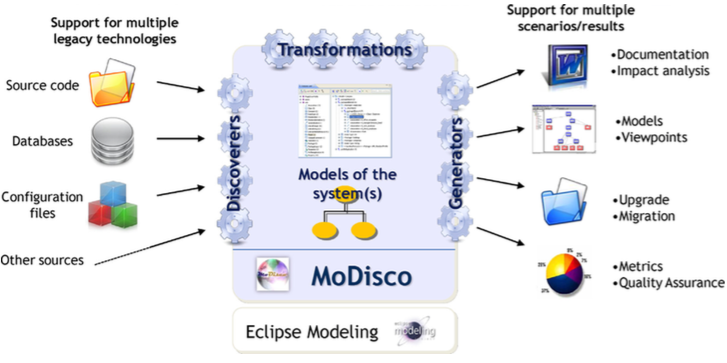
\includegraphics[scale=0.55]{images/modiscoAllArtefacts.png}
	\caption{Visão geral de um projeto MoDisco.}
	\label{fig:modisco_allArtefacts}
	\fadaptada{Bruneliere_2014}
\end{figure}

Contudo, uma das limitações dessa ferramenta é o suporte e a aplicação de refatorações. Observe que, naturalmente, MoDisco não é capaz de aplicar refatorações de forma automática, pois a maioria das refatorações necessitam de interação do usuário para fornecer as informações necessárias. No contexto desta Tese foi utilizado a ferramenta MoDisco para recuperar as informações do código-fonte legado escrito em Java. Sem o auxílio dessa ferramenta todo o sistema legado, escrito em Java, deveria ser transformada em uma instância do KDM de forma manual, o que poderia atrasar esta pesquisa, uma vez que toda a manipulação do KDM foi possível por causa da existência do MoDisCo e do seu suporte em Java para manipular o metamodelo KDM. Por exemplo, não é possível para o MoDisco adivinhar quais refatorações devem ser aplicadas e em quais elementos; tais informações devem ser fornecidas por um usuário.

\section{Considerações Finais}\label{sec:consideracoes_finais}

O foco deste capítulo direciona-se à análise do panorama atual da literatura que trata sobre a modernização de sistemas legados levando em consideração a padronização proposta pela OMG. Neste capítulo foram mostrados os principais conceitos sobre ADM, KDM, bem como seus pacote e camadas que são necessários para facilitar o entendimento dessa Tese e fundamentais ao desenvolvimento da proposta aqui desenvolvida.

Observou-se também que o metamodelo KDM por intermédio de suas camadas, pacotes e metaclasses permite a criação de um modelo independente de plataforma que representam um sistema legado em diversas visões. O objetivo da OMG ao criar esse metamodelo propõe uma padronização da reengenharia de software, fornecendo abstrações que ajudem no processo de reengenharia de sistemas. Além disso, pode-se constatar que diferentemente de metamodelos existentes, tais como a UML, o KDM têm como intuito agrupar todos os artefatos (visões) do sistema em um único metamodelo. Dessa forma, pode-se argumentar que o metamodelo KDM pode ser considerado como uma família de metamodelos, uma vez que o mesmo compartilha uma terminologia consistente e homogenia.

Neste capítulo também foi apresentado sobre a ferramenta MoDisco, uma das principais ferramentas que automatiza a instanciação do metamodelo KDM. Essa ferramenta foi utilizada no contexto deste trabalho para dar suporte à recuperação do modelo KDM a partir de código-fonte legado escrito em Java.

\chapter{Mapeamento Sistemático sobre ADM e KDM}\label{chapter:mapeamento_sistematico}
\section{Considerações Iniciais}

Quando se conduz uma revisão de literatura sem o pré-estabelecimento de um protocolo de revisão há um direcionamento por interesses pessoais, o que leva a resultados pouco confiáveis. Neste contexto, pesquisadores vêm utilizando uma técnica denominada de \sigla{MS}{Mapeamento Sistemático} para auxiliar o pesquisador a conduzir uma revisão bibliográfica de forma totalmente sistemática com o intuito de evitar que trabalhos importantes fiquem fora de suas pesquisas. Um MS é caracterizado por ser um meio de avaliar e interpretar todas as pesquisas disponíveis, referentes a uma questão de pesquisa, tema, área ou fenômeno de interesse. O MS tem como objetivo apresentar uma avaliação justa de um tema de pesquisa, utilizando uma metodologia confiável e rigorosa~\cite{Petersen_2008, Kitchenham_2010, Petersen_20151}.


De acordo com~\citeonline{Petersen_20151} MS são projetados para dar uma visão geral de uma área de investigação por meio da classificação e contagem de contribuições em relação a um conjunto de categorias de classificação~\cite{Petersen_2008, Kitchenham_2010}. Em outras palavras, trata-se de realizar uma vasta pesquisa na literatura, a fim de identificar quais temas já foram abordados na literatura, quais temas ainda não foram abordados e quais são novas possíveis pesquisas~\cite{Kitchenham_2010}. Embora, ambas as técnicas, MS e \sigla{RS}{Revisão Sistemática} compartilhem algumas características - (por exemplo, no que diz respeito à busca e seleção do estudo), segundo~\citeonline{Petersen_20151} tais técnicas são diferentes em termos de objetivos e, portanto, utilizam diferentes abordagens para análise de dados. Enquanto RS visa sintetizar evidências, também considerando a força da evidência, MS preocupa-se principalmente com a estruturação de uma determinada área de pesquisa~\cite{Petersen_20151}. Segundo~\citeonline{Kitchenham_2010} MS implica na forma mais adequada para se identificar, avaliar e interpretar toda uma área de pesquisa para um tema em particular. 

Resume-se que um MS configura um alicerce para novas atividades de pesquisa acerca de um determinado tema. Neste contexto, foi realizado um MS sobre ADM e KDM~\cite{durelli_systematic_mapping}; a motivação para realizar esse MS é identificar os temas que têm sido mais investigados, bem como os temas que ainda não foram pesquisados no contexto da abordagem ADM e o metamodelo KDM. Embora, a ADM seja uma abordagem relativamente nova, o OMG afirma que ela é uma importante abordagem, pois combina dois dos principais campos da Engenharia de Software: MDE (ver Capítulo~\ref{chapter:fundamentacao_teorica}, Seção~\ref{Cap2_Sec2_Desenvolvimento_Dirigido_a_Modelos}) e reengenharia de software. Desde a criação da ADM muitos esforços têm enfatizado a modernização de sistemas por meio desta abordagem. Assim, se faz necessário a condução de uma investigação mais sistemática dos temas englobados por esta área de pesquisa. Nota-se que esse capítulo é uma extensão do seguinte artigo: \textit{A Mapping Study on Architecture-Driven Modernization}~\cite{durelli_systematic_mapping}.


Este capítulo está organizado da seguinte forma: Seção~\ref{sec:metodologia_pesquisa} descreve a metodologia de como o MS foi conduzido. Subseção~\ref{subsec:estrategia_de_busca} apresenta a estratégia de busca utilizada nesse MS. A Subseção~\ref{subsec:fonte_de_estudo_e_selecao} descreve as fontes de estudos utilizadas no MS, além disso, também apresenta como foi realizado a seleção dos estudos. Subseção~\ref{subsec:definindo_esquema_de_classificacao} apresenta o esquema de classificação considerado no MS. Na Subseção~\ref{subsec:extracao_e_sintese_do_dados} a extração e síntese dos dados são discutidas. Na Subseção~\ref{subsec:mapeamento_e_dis} um gráfico de bolha resultante do MS é apresentado, dando ênfase nas principais descobertas desse MS. Ainda nessa subseção as questões de pesquisas são discutidas. A Seção~\ref{subsec:principais_constatações_e_questões_Em_Aberto} apresenta as principais constatações e questões em aberto relacionadas a ADM e KDM. Seção~\ref{subsec:ameaças_a_validade} apresenta as ameaças à validade do MS. Finalmente, Seção~\ref{sec:considerações_finais_do_mapeamento_sistematico} descreve as considerações finais desse capítulo.


%Seção X apresenta as principais descobertas desse MS. Na Seção X as ameaças às validades são apresentadas. Na Seção X as considerações finais são destacadas.\change{mudar e colocar a estrutura}

\section{Metodologia de Pesquisa}\label{sec:metodologia_pesquisa}

Como já salientado nas considerações iniciais um MS fornece um processo sistemático para identificar relevantes pesquisas com o objetivo de responder específicas questões. Durante a condução deste MS todos os passos propostos por~\citeonline{Petersen_20151, Petersen_2008} foram seguidos. Uma visão geral de todos os passos propostos por tais autores pode ser observada na Figura~\ref{fig:all_steps_MS}. Nota-se que cada passo produz um resultado intermediário, como visualizado na Figura~\ref{fig:all_steps_MS}. De acordo com tais autores, cinco passos essenciais são: (\textit{i}) \textit{Definition of Research Questions}, (\textit{ii}) \textit{Conducting Search}, (\textit{iii}) \emph{Screening of Papers}, (\textit{iv}) \emph{Keywording using Abstracts} e (\textit{v}) \textit{Data Extraction and Mapping Process}. 

\begin{figure}[h]
 \caption{Processo para a condução de um Mapeamento Sistemático}
 \label{fig:all_steps_MS}
 \centering
 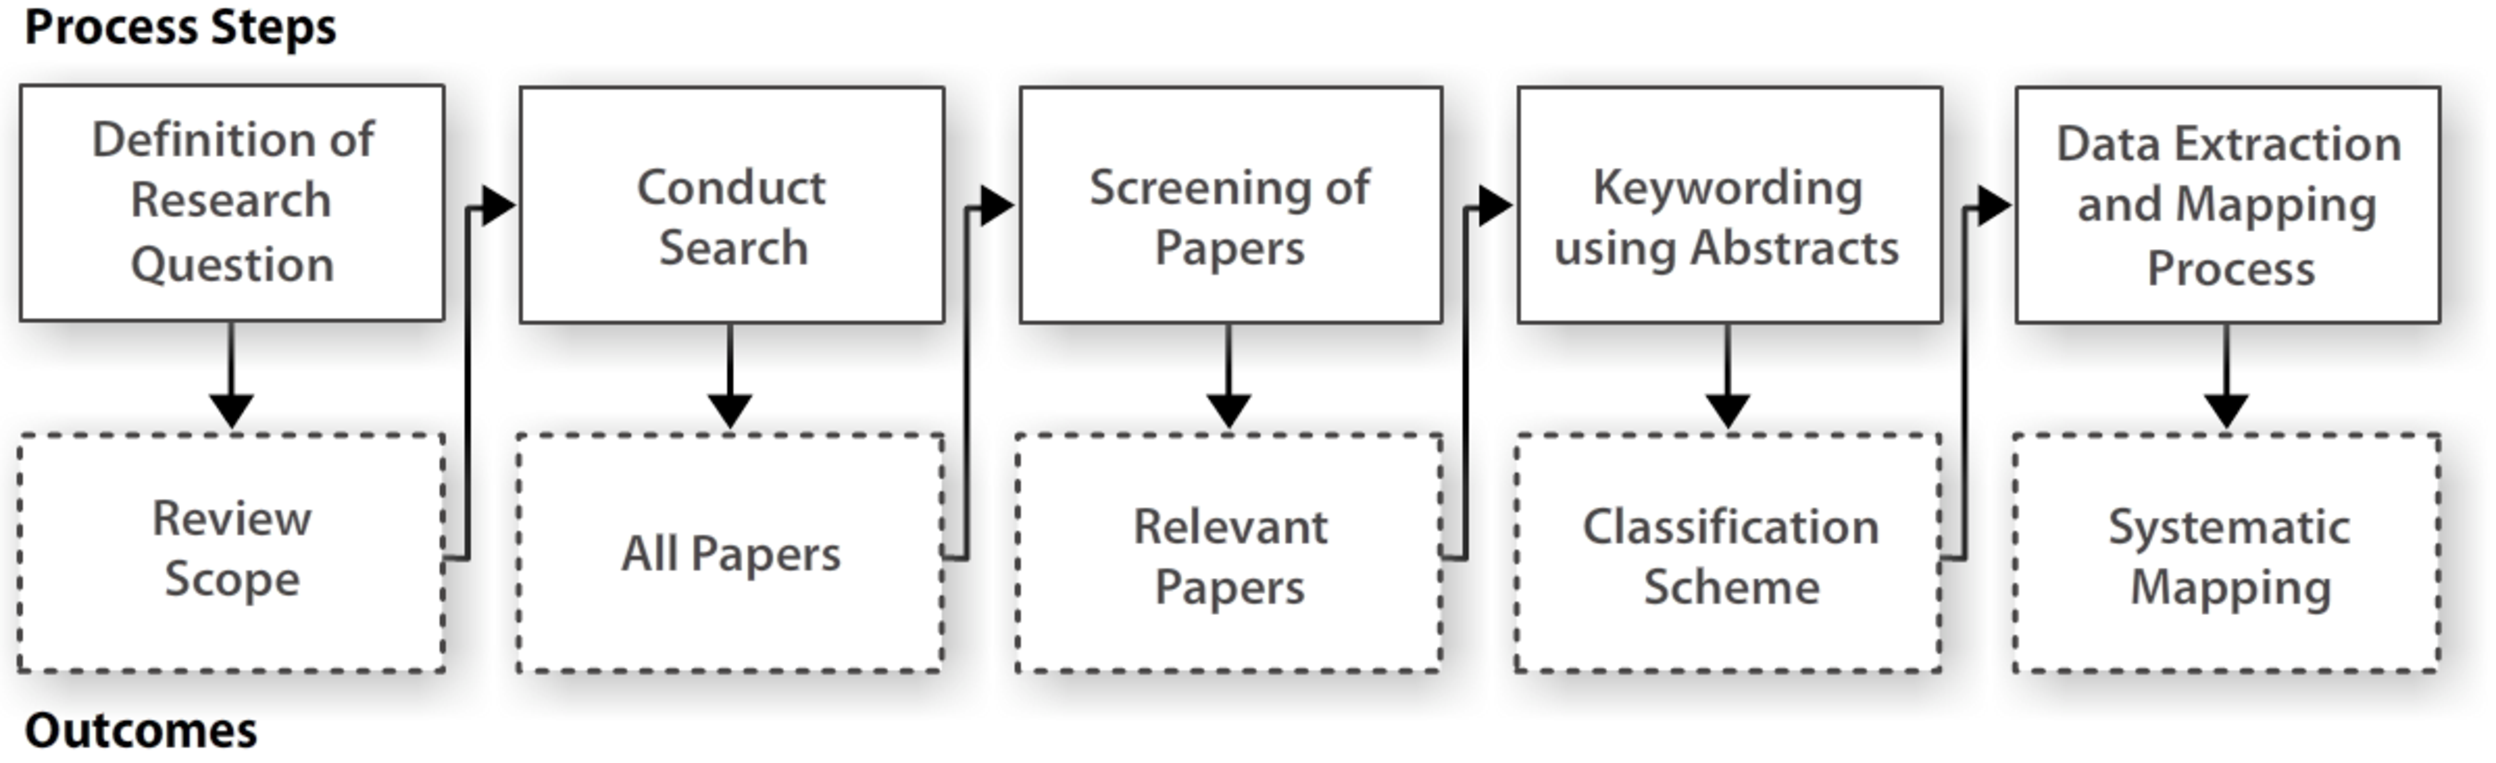
\includegraphics[scale=0.3]{images/systematic_mapping_process}
 \fadaptada{Petersen_2008}
\end{figure}

\subsection{Estratégia de Busca}\label{subsec:estrategia_de_busca}

O protocolo do MS é definido neste passo - esse protocolo usualmente é dividido em dois sub-passos: (\textit{i}) a definição das questões de pesquisa e (\textit{ii}) a \textit{string} de busca. 

\sigla{QPs}{Questões de Pesquisas} devem englobar o propósito do MS. O objetivo do MS é a identificação e a caracterização do estado atual da ADM e do metamodelo KDM. Dessa forma, a motivação para realizar esse MS é identificar os temas que têm sido mais investigados, bem como os temas que ainda não foram investigados no contexto da abordagem ADM e o metamodelo KDM. A partir desse objetivo, delineiam-se as seguintes questões:

\begin{itemize}
\item \textbf{QP$_1$} - Dado os metamodelos da ADM, qual metamodelo tem sido mais utilizado na literatura? Além disso, dado o metamodelo identificado, qual (is) é (são) o (s) pacote (s) mais e menos utilizado (s)?
\item \textbf{QP$_2$} - Que tipos de estudos têm sido publicados no contexto da ADM?
\item \textbf{QP$_3$} - Quais são as áreas que têm sido mais e menos investigadas no contexto da ADM? Adicionalmente, quais são os tipos de contribuições que foram publicadas até agora?
\end{itemize}

Considerando as QPs estabelecidas, definiram-se os atributos e a amplitude do MS com a técnica \sigla{PICO}{\textit{Population}, \textit{Intervention}, \textit{Comparator} e \textit{Outcomes}}~\cite{Kitchenham_2010} e identificaram-se termos a serem utilizados na \textit{string} de busca:

\begin{itemize}
\item Quanto à população: Em Engenharia de Software e no contexto de MS, população diz respeito à uma específica área de pesquisa. No contexto deste MS a população são artigos publicados na literatura científica sobre algum processo, técnica ou ferramenta que utilize ADM e seus metamodelos;

\item Quanto à intervenção: Em Engenharia de Software, intervenção refere-se à metodologia de software, ferramenta, tecnologia ou procedimento. No contexto, deste MS a intervenção são abordagens e ferramentas publicadas na literatura científica que utilizam ADM e seus metamodelos;

\item Quanto à comparação: A comparação não é aplicada no contexto deste MS;

\item Quanto aos resultados esperados: Espera-se como resultado uma visão geral dos estudos que foram publicados para a ADM e seus metamodelos, enfatizando estudos primários que descrevem técnicas, abordagens, processos e ferramentas para auxiliar o engenheiro de modernização durante a condução de modernização de sistemas legados com a utilização da abordagem ADM.

\end{itemize}

A partir dos termos identificados, define-se a \textit{string} de busca para a recuperação de estudos. Todos os termos devem ser traduzidos de acordo com o idioma dos artigos que se deseja recuperar (no contexto deste MS, inglês) e associados com sinônimos, conforme sugestões de especialistas. Na Figura~\ref{fig:string_de_busca} é apresentada a \textit{string} de busca que foi utilizada neste MS.

\begin{figure}[h]
 \caption{\textit{String} de busca definida.}
 \label{fig:string_de_busca}
 \centering
 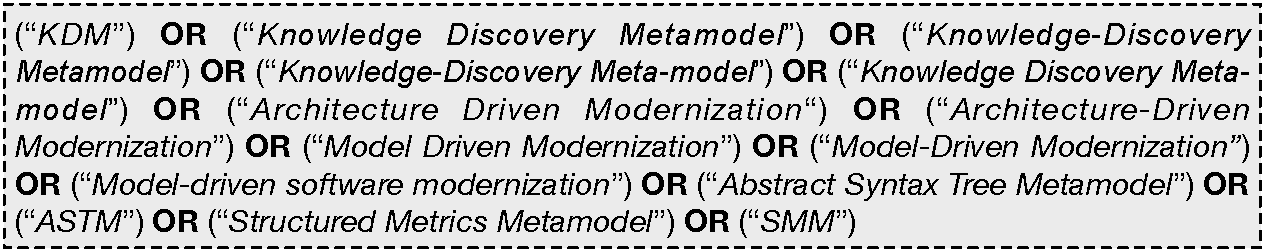
\includegraphics[scale=0.6]{images/searchStringMS}
 \fautor
\end{figure}

\subsection{Fonte de Estudos e Seleção dos Estudos}\label{subsec:fonte_de_estudo_e_selecao}

As fontes de estudos utilizadas durante o MS foram as bibliotecas digitais da \textit{ACM}, 
\textit{IEEE XPLORE}, \textit{Scopus}, \textit{Web of Science} e \textit{Engineering Village}. Tais bibliotecas digitais foram selecionadas com base na experiência reportada por~\citeonline{dyba_2015}. De acordo com esses autores, tais fontes de estudos são suficientes para identificar estudos primários relevantes. Nota-se que os recursos fornecidos por essas bibliotecas digitais, bem como a sintaxe exata da \textit{string} de busca a ser aplicada, variam de uma biblioteca para outra, assim, a \textit{string} de busca apresentada na Figura~\ref{fig:string_de_busca} foi utilizada como base para construir uma \textit{string} de busca semanticamente equivalente e sob medida para cada biblioteca digital. %As \textit{strings} de buscas utilizada em todas as bibliotecas digitais pode ser visualizada na Tabela~\ref{long}.


%\begin{longtable}[!tb]{ | m{2cm} | m{12cm}| }
% \caption{Bibliotecas digitais e \textit{String} de busca adaptadas.\label{long}}\\
 
% \hline
% \multicolumn{2}{| c |}{Início da Tabela}\\
% \hline
% Bibliotecas Digitais & \textit{String} de Busca\\
% \hline
% \endfirsthead
 
% \hline
% \multicolumn{2}{|c|}{Continuação da Tabela~\ref{long}}\\
% \hline
% Bibliotecas Digitais & \textit{String} de Busca\\
% \hline
% \endhead
 
% \hline
% \endfoot
 
% \hline
% \multicolumn{2}{| c |}{Fim da Tabela}\\
% \hline\hline
% \endlastfoot
 
% ACM & ("Knowledge Discovery Metamodel" or "Knowledge-Discovery Metamodel" or "Knowledge-Discovery Meta-model" or "Knowledge Discovery Meta-model" or "Architecture Driven Modernization" or "Architecture-Driven Modernization" or "Model Driven Modernization" or "Model-Driven Modernization" or "Model-driven software modernization" or "ADM Pattern Recognition specification" or "ADM Visualization specification" or "ADM Refactoring specification" or "ADM Transformation specification" or "KDM Metamodel" or "KDM Meta-model" or "Software Metrics Meta-model" or "Software Metrics Metamodel" or "Structured Metrics Meta-Model" or "Structured Metrics Metamodel" or "Abstract Syntax Tree Metamodel" or "Abstract Syntax Tree Meta-model")\\
 %\hline
 %IEEE XPLORE & ((((((((((((((((((((("Knowledge Discovery Metamodel") OR "Knowledge-Discovery Metamodel") OR "Knowledge-Discovery Meta-model") OR "Knowledge Discovery Meta-model") OR "Architecture Driven Modernization") OR "Architecture-Driven Modernization") OR "Model Driven Modernization") OR "Model-Driven Modernization") OR "Model-driven software modernization") OR "ADM Pattern Recognition specification") OR "ADM Visualization specification") OR "ADM Refactoring specification") OR "ADM Transformation specification") OR "KDM Metamodel") OR "KDM Meta-model") OR "Software Metrics Meta-model") OR "Software Metrics Metamodel") OR "Structured Metrics Meta-Model") OR "Structured Metrics Metamodel") OR "Abstract Syntax Tree Metamodel") OR "Abstract Syntax Tree Meta-model")\\
 %\hline
 %Scopus & ("Knowledge Discovery Metamodel"  OR  "Knowledge-Discovery Metamodel"  OR  "Knowledge-Discovery Meta-model"  OR  "Knowledge Discovery Meta-model"  OR  "Architecture Driven Modernization" OR  "Architecture-Driven Modernization"  OR  "Model Driven Modernization"  OR  "Model-Driven Modernization"  OR  "Model-driven software modernization"  OR  "ADM Pattern Recognition specification"  OR  "ADM Visualization specification"  OR  "ADM Refactoring specification"  OR  "ADM Transformation specification"  OR  "KDM Metamodel"  OR  "KDM Meta-model"  OR  "Software Metrics Meta-model"  OR  "Software Metrics Metamodel"  OR  "Structured Metrics Meta-Model"  OR  "Structured Metrics Metamodel"  OR  "Abstract Syntax Tree Metamodel"  OR  "Abstract Syntax Tree Meta-model")\\
 %\hline
 %Web of Science & ("Knowledge Discovery Metamodel" OR "Knowledge-Discovery Metamodel" OR "Knowledge-Discovery Meta-model" OR "Knowledge Discovery Meta-model" OR "Architecture Driven Modernization" OR "Architecture-Driven Modernization" OR "Model Driven Modernization" OR "Model-Driven Modernization" OR "Model-driven software modernization" OR "ADM Pattern Recognition specification" OR "ADM Visualization specification" OR "ADM Refactoring specification" OR "ADM Transformation specification" OR "KDM Metamodel" OR "KDM Meta-model" OR "Software Metrics Meta-model" OR "Software Metrics Metamodel" OR "Structured Metrics Meta-Model" OR "Structured Metrics Metamodel" OR "Abstract Syntax Tree Metamodel" OR "Abstract Syntax Tree Meta-model")\\
 %\hline
 %Engeneering Village & "Knowledge Discovery Metamodel" OR "Knowledge-Discovery Metamodel" OR "Knowledge-Discovery Meta-model" OR "Knowledge Discovery Meta-model" OR "Architecture Driven Modernization" OR "Architecture-Driven Modernization" OR "Model Driven Modernization" OR "Model-Driven Modernization" OR "Model-driven software modernization" OR "ADM Pattern Recognition specification" OR "ADM Visualization specification" OR "ADM Refactoring specification" OR "ADM Transformation specification" OR "KDM Metamodel" OR "KDM Meta-model" OR "Software Metrics Meta-model" OR "Software Metrics Metamodel" OR "Structured Metrics Meta-Model" OR "Structured Metrics Metamodel" OR "Abstract Syntax Tree Metamodel" OR "Abstract Syntax Tree Meta-model"\\
 %\hline
 %Google Scholar & ("Knowledge Discovery Metamodel" or "Knowledge-Discovery Metamodel" or "Knowledge-Discovery Meta-model" or "Knowledge Discovery Meta-model" or "Architecture Driven Modernization" or "Architecture-Driven Modernization" or "Model Driven Modernization" or "Model-Driven Modernization" or "Model-driven software modernization" or "ADM Pattern Recognition specification" or "ADM Visualization specification" or "ADM Refactoring specification" or "ADM Transformation specification" or "KDM Metamodel" or "KDM Meta-model" or "Software Metrics Meta-model" or "Software Metrics Metamodel" or "Structured Metrics Meta-Model" or "Structured Metrics Metamodel" or "Abstract Syntax Tree Metamodel" or "Abstract Syntax Tree Meta-model")\\
 %\hline
 %\end{longtable}

Para determinar quais estudos primários são relevantes para responder as QPs, definiu-se um conjunto de critérios de inclusão. Os critérios de inclusão que foram definidos são:

\begin{itemize}
\item Critérios de Inclusão:
    \begin{itemize}
    \item O estudo primário apresenta pelo menos uma abordagem de modernização que utiliza ADM e seus metamodelos;
    \item O estudo primário descreve uma avaliação empírica da abordagem que utiliza ADM.
    \end{itemize}
\end{itemize}

Similarmente, também foram definidos três critérios de exclusão, a saber:

\begin{itemize}
\item Critérios de Exclusão:
    \begin{itemize}
    \item Artigos que menciona ADM e seus metamodelos apenas no \textit{abstract};
    \item Artigos introdutórios para livros e \textit{workshops};
    \item O estudo primário é um artigo pequeno (\textit{short paper}), o qual contém até três páginas.
    \end{itemize}
\end{itemize}

A Scopus foi a biblioteca digital que retornou mais estudos primários, 58\% (150) (ver Figura~\ref{fig:distribuicao_biblioteca_digital}). Por outro lado, foram recuperados 20\% (51) estudos da ACM, 12\% (30) da Engineering Village, 6\% (17) da Web of Science e 4\% (11) da IEEE. 

\begin{figure}[h]
 \caption{Distribuição dos estudos primários de cada biblioteca digital.}
 \label{fig:distribuicao_biblioteca_digital}
 \centering
 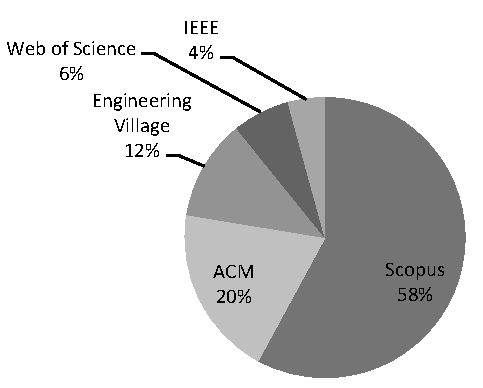
\includegraphics[scale=0.9]{images/retornoDasBasesMS}
 \fautor
\end{figure}

Somando todas as bibliotecas digitais, obteve-se 259 estudos primários no primeiro passo, como ilustrado na Figura~\ref{fig:todos_os_passos}. Após o primeiro passo (ver Figura~\ref{fig:todos_os_passos}), 82 artigos foram selecionados. Nota-se que apenas publicações de conferências e \textit{journals} foram consideradas nesse MS. Posteriormente, os critérios de inclusão anteriormente apresentados foram aplicados para todos os 82 artigos selecionados. Após esse passo, 30 estudos primários foram considerados para serem analisados no MS como mostrado na Figura~\ref{fig:todos_os_passos}.

\begin{figure}[h]
 \caption{Todos os passos conduzidos no MS.}
 \label{fig:todos_os_passos}
 \centering
 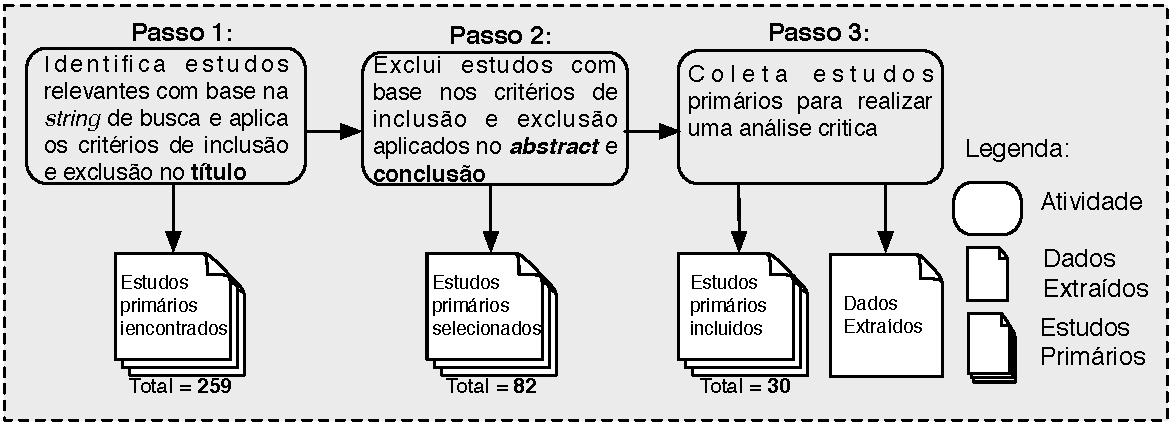
\includegraphics[scale=0.7]{images/todosOsPassosMS}
 \fautor
\end{figure}

\subsection{Definindo um Esquema de Classificação}\label{subsec:definindo_esquema_de_classificacao}

O esquema de classificação utilizado neste MS foi o esquema proposto por~\citeonline{Petersen_2008, Petersen_20151}. Esse esquema classifica cada publicação entre categorias de acordo com três perspectivas: (\textit{i}) \textbf{Área de Foco}, (\textit{ii}) \textbf{Tipo de Contribuição} e (\textit{iii}) \textbf{Tipo de Pesquisa}. O esquema de classificação resultante é descrito a seguir:

\begin{itemize}
\item \textbf{Área de Foco}: Após ler os estudos primários foram identificados cinco principais áreas de foco. 
    
    \begin{itemize}
        \item \aspas{\textbf{Modernização de Software}}: essa área de foco está relacionada com estudos primários que descrevem abordagens que empregam ADM para modernizar sistemas legados para outra plataforma ou arquitetura;
        \item \aspas{\textbf{Extração de \textit{Business Knowledge}}}: descrevem estudos primários que apresentam processos, métodos ou abordagens para extrair informações de negocio de sistemas legados;
        \item \aspas{\textbf{Extração de Interesse}}: representam estudos primários que descrevem processos, métodos ou abordagens para extrair interesses transversais de sistemas legados;
        \item \aspas{\textbf{Extensão dos metamodelos da ADM}}: descrevem estudos primários que apresentam abordagens, métodos ou processos para estender um determinado metamodelo da ADM;
        \item \aspas{\textbf{Aplicabilidade}}: incluem estudos primários que têm como objetivo representar evidência da utilização da ADM e seus metamodelos na prática, ou seja, artigos que apresentam pesquisas ou relatórios para facilitar o entendimento da ADM e seus metamodelos.
    \end{itemize}
    
    \item \textbf{Tipo de Contribuição}: Similarmente, também foram identificados cinco tipos de contribuições:
        
        \begin{itemize}
            \item \aspas{\textbf{Ferramentas}}: estudos primários que apresentam ferramentas para auxiliar a modernização de sistemas legados utilizando ADM e seus metamodelos;
            \item \aspas{\textbf{Processo}}: refere-se a estudos primários que descrevem processos para auxiliar a modernização de sistemas legados utilizando ADM e seus metamodelos;
            \item \aspas{\textbf{Transformação de Modelos}}: agrupa estudos primários que descrevem o uso de linguagens de transformações para realizar transformações entre os metamodelos da ADM;
            \item \aspas{\textbf{Metamodelos}}: estudos primários que relatam extensão nos metamodelos da ADM para suprir um específico problema, por exemplo, fornecer uma extensão leve para o metamodelo KDM para representar o paradigma orientado a aspecto;
            \item \aspas{\textbf{Métricas}}: refere-se a estudos primários que se concentram em propor ou aplicar métricas para medir a eficácia de ADM e seus metamodelos.
        \end{itemize}
        
        \item \textbf{Tipo de Pesquisa}: Tipo de pesquisa reflete a abordagem de pesquisa que foi utilizada no estudo primário. Assim, essa categoria foi criada com base no esquema proposto por~\citeonline{Wieringa_2005}.
        
        \begin{itemize}
            \item \aspas{\textbf{Pesquisa de validação}}: tem por objetivo analisar uma proposta de solução que ainda não foi aplicado na prática. A validação é realizada de uma forma sistemática e pode apresentar qualquer um destes: protótipos, análise matemática, etc;
            \item \aspas{\textbf{Pesquisa de avaliação}}: em contraste com a pesquisa de validação, pesquisa de avaliação visa examinar uma solução que já foi praticamente aplicada. Estudos nesta categoria investigam a aplicação na prática da solução proposta e, geralmente, os resultados obtidos utilizando estratégias empíricas (por exemplo, experimentos e estudo de casos);
            \item \aspas{\textbf{Proposta conceitual}}: apresenta um arranjo de ver as coisas que já existem, de uma nova maneira. No entanto isso não resolve precisamente um problema particular. Podem incluir taxonomias, referenciais teóricos, etc;
            \item \aspas{\textbf{Artigo descrevendo experiência}}: artigos que descrevem sobre a experiência pessoal do autor para um ou mais projetos. O autor geralmente apresenta como e o que foi realizado no projeto;
            \item \aspas{\textbf{Artigo descrevendo opinião}}: artigos que descrevem a opinião pessoal do autor sobre a adequação ou inadequação de uma técnica ou ferramenta específica.
        \end{itemize}
    
\end{itemize}


\subsection{Extração e Síntese dos Dados}\label{subsec:extracao_e_sintese_do_dados}

Os 30 estudos selecionados na etapa anterior foram analisados. Assim, criou-se um formulário para auxiliar a extração de dados. Esse formulário contém os seguintes dados: (\textit{i}) dados relevantes sobre como a ADM e seus metamodelos estão sendo utilizados na literatura, (\textit{ii}) a data de quando a extração do dado foi realizada, (\textit{iii}) o título do estudo primário, (\textit{iv}) os autores do estudo primário, (\textit{v}) o veículo de publicação e (\textit{vi}) um resumo destacando as principais contribuições do estudo primário para posteriormente realizar a classificação. Durante o processo de extração, dados sobre cada estudo primário foram independentemente coletados por todos os pesquisados que participaram do MS. É importante destacar que a primeira execução desse MS foi realizada em Novembro de 2013, posteriormente, o MS foi conduzido novamente em Agosto de 2015 com o objetivo de atualizar o MS.

\subsection{Mapeamento e discussão das QPs}\label{subsec:mapeamento_e_dis}

O foco desta seção é apresentar uma visão geral de como a ADM e seus metamodelos estão sendo pesquisados e utilizados na literatura, bem como identificar possíveis grupos de evidências (ou seja, onde pode haver margem para uma literatura mais completa) e deserto de evidências (ou seja, onde melhor ou nova pesquisa é necessária) de pesquisas. Além de apresentar essa visão geral, esta seção também tem como objetivo apresentar respostas para as QPs definidas anteriormente.

Em vez de utilizar tabelas de frequência foi produzido um gráfico de bolha para reportar a frequência e distribuição dos estudos primários selecionados de acordo com suas categorias e data de publicação. Argumenta-se que esse gráfico de bolha representa um mapa geral de como ADM e seus metamodelos têm sido utilizados na literatura. O mapa resultante é apresentado na Figura~\ref{fig:mapa_mapeamento_sistematico}.


\begin{figure}[h]
 \caption{Visão geral da pesquisa sobre ADM e seus metamodelos.}
 \label{fig:mapa_mapeamento_sistematico}
 \centering
 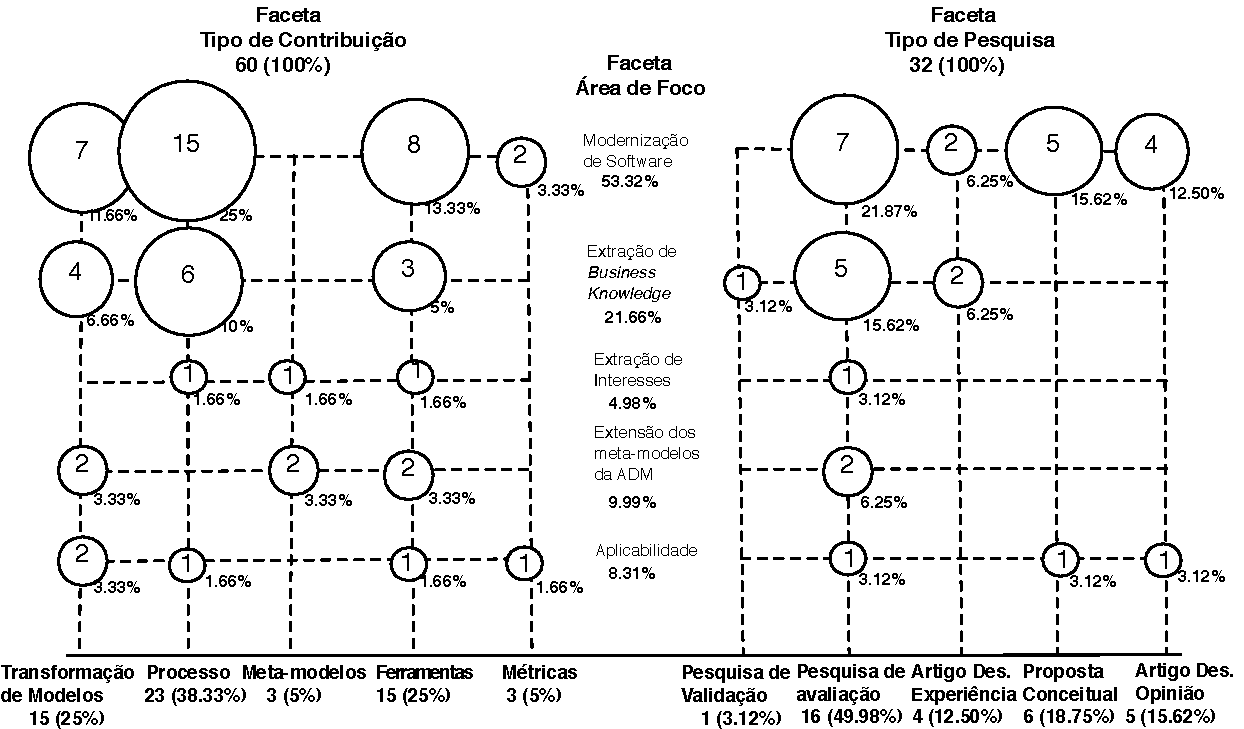
\includegraphics[scale=0.8]{images/MapaMS_port}
 \fautor
\end{figure}

Como pode ser observado esse gráfico de bolha contém dois vértices, X e Y, os quais possuem bolhas em cada categoria. Nota-se que o tamanho de cada bolha representa o número de estudos primários que foram classificados a uma categoria específica. Este gráfico é um resumo visual e fornece uma visão panorâmica que permite identificar quais são as categorias que foram salientadas em pesquisas anteriores, além disso, é possível identificar facilmente lacunas e oportunidades para futuras pesquisas. O gráfico de bolha apresentado na Figura~\ref{fig:mapa_mapeamento_sistematico} contém três facetas: \textbf{Tipo de Contribuição}, \textbf{Área de Foco} e \textbf{Tipo de Pesquisa}. Embora 30 estudos primários foram considerados nesse MS é importante mencionar que para o gráfico de bolha alguns estudos primários foram agrupados em mais de uma categoria. Por exemplo, para o gráfico de bolha apresentado na Figura~\ref{fig:mapa_mapeamento_sistematico} a soma dos estudos primários agrupados em cada faceta é maior do que o número de estudos primários selecionados, isso acontece uma vez que um determinado estudo primário pode ser classificado em diversas facetas e categorias.

Para responder a primeira parte da \textbf{QP$_1$} foram analisados todos os estudos primários, concentrando-se na identificação de qual metamodelo da ADM tem sido mais utilizado na literatura. Na Figura~\ref{fig:frequencia_kdm_packages}, lado esquerdo, são apresentados os metamodelos da ADM que são utilizadas na literatura. Como pode ser observado o metamodelo KDM é o metamodelo que é mais utilizado, tendo uma frequência de 66.67\%. Em seguida, o segundo metamodelo mais utilizado é o SMM, 10\% dos estudos primários relatam a utilização desse metamodelo. Enquanto o metamodelo ASTM foi utiliza em apenas 6.66\% dos estudos primários. 16.66\% dos estudos primários não mencionam explicitamente qual metamodelo foi utilizado durante o processo de modernização conduzido, apenas citam e relatam a utilização da ADM.

\begin{figure}[!h]
\caption{Frequência de utilização dos metamodelos da ADM e frequência de utilização dos seus pacotes.}
 \label{fig:frequencia_kdm_packages}
\centering
\begin{minipage}{.5\textwidth}
  \centering
  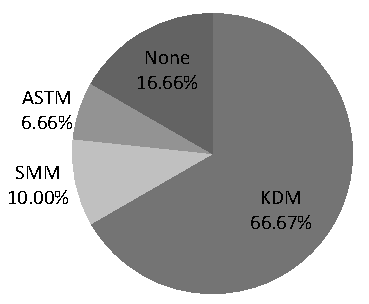
\includegraphics[scale=0.9]{images/MetamodelosDIstribuition}
\end{minipage}%
\begin{minipage}{.5\textwidth}
  \centering
  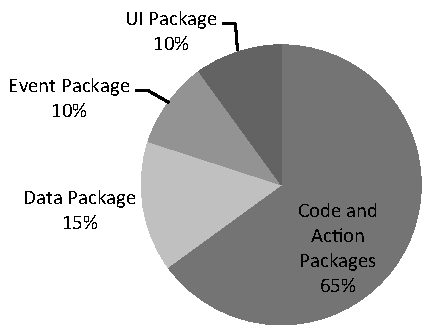
\includegraphics[scale=0.9]{images/PacotesKDM}
\end{minipage}
\fautor
\end{figure}

Para responder a segunda parte da \textbf{QP$_1$} foram analisados quais são os pacotes que são mais e menos utilizados dentro do metamodelo KDM. Na Figura~\ref{fig:frequencia_kdm_packages}, lado direito, é evidente que os pacotes \texttt{Code} e \texttt{Action} são os mais utilizados na literatura, contendo uma frequência de 65\%. Acredita-se que a razão para essa frequência tão alta seja por dois principais motivos: (\textit{i}) tais pacotes representam o código-fonte de um determinado sistema, além disso, a maioria das abordagens identificadas utiliza como entrada o código-fonte de sistemas que almejam modernizar seguindo a ADM e seus metamodelos; e (\textit{ii}) outros pacotes do KDM ainda não possuem ferramentas para realizar a instanciação de forma automática, ou seja, existe uma limitação de \textit{parsers} que análise outros tipos de artefatos de um determinado sistema para criar uma representação mais fiel do sistema, não apenas do código-fonte. O terceiro pacote mais utilizado é o \texttt{Data}, o qual é utilizado para representar dados - tais como banco de dados, registros, etc. Os pacotes \texttt{Event} e \texttt{UI} ambos foram utilizados 10\%. Outros pacotes do metamodelo KDM não foram explicitamente mencionados nos estudos primários identificados.

Observando a faceta \textbf{Tipo de Pesquisa}, lado direito da Figura~\ref{fig:mapa_mapeamento_sistematico}, é possível responder a \textbf{QP$_2$}. A maioria dos estudos primários identificados foi classificado como \aspas{\textbf{Pesquisa de Avaliação}}, aproximadamente 49\%. Uma pequena porcentagem de estudos primários foi classificado como \aspas{\textbf{Pesquisa de Validação}}, apenas 3.12\%. 12.50\% dos estudos primários identificados descrevem a experiência dos autores (\aspas{\textbf{Artigo Des. Experiência}}) com a utilização da ADM e seus metamodelos. 18.75\% foram agrupas em \aspas{\textbf{Proposta Conceitual}} e \aspas{\textbf{Artigos Des. Opinião}} teve a frequência de 15.62\%.

Ainda em relação à Figura~\ref{fig:mapa_mapeamento_sistematico} na faceta \textbf{Tipo de Contribuição}, lado esquerdo, pode-se observar que a maioria dos estudos primários identificados apresenta \aspas{\textbf{processos}} para auxiliar os engenheiros de software durante a modernização de sistemas legados. Também foi identificado um total de 15 estudos primários (25\%) que apresentam algum tipo de \aspas{\textbf{transformação de modelos}} utilizando os metamodelos da ADM. Similarmente, 15 estudos primários (25\%) apresentam ferramentas para auxiliar o engenheiro de software durante a condução da modernização utilizando ADM e seus metamodelos. Acredita-se que esses dois últimos resultados foram obtidos uma vez que a maioria dos estudos primários identificados descreve processos de modernização, assim, pesquisadores devem criar um conjunto de transformações de modelos e ferramentas para automatizar parcialmente ou totalmente o processo proposto.

Por outro lado, \aspas{\textbf{metamodelos}} e \aspas{\textbf{métricas}} são as contribuições com menos estudos primários identificados, 5\% cada. Assim, argumenta-se que os estudos primários que descrevem \aspas{\textbf{processos}} para ajudar a modernização dos sistemas legados por meio da ADM, estudos que apresentam \aspas{\textbf{transformação de modelos}} entre os metamodelos da ADM (KDM, SMM e ASTM) e artigos que descrevem ferramentas para automatizar parcialmente ou totalmente o processo da ADM pode ser considerado como grupos de evidências. Enquanto que \aspas{\textbf{metamodelos}} (ou seja, artigos que explicam e/ou apresentam como estender metamodelos da ADM) e \aspas{\textbf{métricas}} (artigos que descrevem como aplicar métricas nos metamodelos da ADM) podem ser considerados como deserto de evidência, assim, novos estudos primários são necessários.

Considerando o centro da Figura~\ref{fig:mapa_mapeamento_sistematico}, faceta \textbf{Área de Foco} é possível visualizar que a maioria dos estudos primários identificados foi classificado como \aspas{\textbf{Modernização de Software}}, um total de 53.32\%. Em seguida, 21.66\% dos estudos primários foram categorizados em \aspas{\textbf{Extração de \textit{Business Knowledge}}}. \aspas{\textbf{Extração de Interesses}}, \aspas{\textbf{Extensão dos metamodelos da ADM}} e \aspas{\textbf{Aplicabilidade}} coletivamente representam uma porcentagem de aproximadamente 25\% dos estudos primários. Como resultado dessa análise foi possível responder parcialmente a \textbf{QP$_3$}, ou seja, os principais \textbf{Tipo de Contribuição} relacionado à ADM e seus metamodelos disponíveis na literatura e identificadas neste MS foram destacadas. A resposta conclusiva e completa da \textbf{QP$_3$} é apresenta a seguir. Para facilitar o entendimento e a organização deste mapeamento cada \textbf{Área de Foco} identificado no MS é apresentado em uma subseção.


\subsubsection{Modernização de Software} % (fold)
\label{ssub:approach}

\citeonline{6311013} propõem \textbf{GAFEMO}, a qual é uma abordagem para auxiliar a modernizar sistemas legados em sistemas orientados a serviço. Essa abordagem utiliza como entrada o sistema legado e então cria uma instância do metamodelo KDM para representar o código-fonte do sistema legado. Posteriormente, os autores definiram um conjunto de transformações para serem aplicadas nessa instância do KDM para criar os serviços.


 %Jorge Maratalla et al., propose \textbf{GAFEMO}~\cite{6311013}, which aims to modernize a legacy systems to the service-oriented approach taking advantage of the features provided by gap-analysis techniques. This approach takes as input a legacy system and then creates KDM representations of it. Afterwards, a set of rules are applied in this model to create the services.

%In~\cite{Mazon:2007:MDM:1784489.1784497} the authors propose a modernization approach for the modernization of Data warehouses following the concepts of ADM. The approach automatically performs the following tasks: (\textit{i}) obtain a logical representation of data sources (\textit{ii}) mark this logical representation with MD concepts, and (\textit{iii}) derive a conceptual MD model from the marked model.

%\citeonline{Mazon:2007:MDM:1784489.1784497} apresentam uma abordagem para modernizar

\citeonline{Mazon:2007:MDM:1784489.1784497} definiram uma abordagem para modernizar \textit{data warehouses} seguindo os conceitos da ADM. Essa abordagem automaticamente executa as seguintes tarefas: (\textit{i}) obtém uma representação logica das fontes de dados; (\textit{ii}) posteriormente, essa representação lógica é anotada e transformada em instância do KDM; (\textit{iii}) em seguida a instância do KDM é transformada em um modelo de análise de dados multidimensional. Similarmente, \citeonline{Guzman:2007:AAR:1339262.1339532} definem uma abordagem para realizar a análise de sistemas legados e criar funcionalidades para ser exposto como serviços usando conceitos de \textit{Web Services} juntamente com a ADM.



%In~\cite{Guzman:2007:AAR:1339262.1339532} is defined an approach that is focused on the analysis of legacy systems to discover and create functionalities to be exposed as services using Web Services by means of ADM. 
%It is based in five steps: (\textit{i}) Database reverse engineering: database schema is reversed and a suitable model is built; (\textit{ii}) First service extraction: based on the structure of the database schema, a first service extraction can be undertaken; (\textit{iii}) PIM generation: is obtained from the PSM representation using a model-to-model transformation, CRUD operations are automatically created; (\textit{iv}) Service discovering: abstract objects are identified in the PIM; (\textit{v}) WSDL (Web Service Description Language) generation: using the PIM, a model-to-model transformation and a WSDL  metamodel are generated to expose the services discovered and created in the PIM and the PSM. 

Em~\citeonline{5741334, SMR:SMR582} os autores desenvolveram uma abordagem seguindo as diretrizes da ADM denominada \aspas{CloudMIG}. Essa abordagem tem como objetivo fornecer software como serviço (do inglês - \sigla{SaaS}{\textit{Software as a Service}}). %Essa abordagem consiste de seis principais passos: (\textit{i}) extração: inclui a extração da arquitetura e instanciação do sistema em nível do metamodelo KDM, (\textit{ii}) seleção: 
Do mesmo modo, \citeonline{4400179} também desenvolveu uma abordagem para utilizar ADM e seus metamodelos, principalmente o KDM, para analisar sistemas legados e descobrir e criar funcionalidades para serem expostas como serviços utilizando os conceitos de \textit{Web Services}.

%In~\cite{5741334, SMR:SMR582} is proposed an approach based on ADM named CloudMIG that aims at supporting SaaS (Software as a Service) providers to semi-automatically migrate legacy software systems to the cloud. It is composed of six major steps: (\textit{i}) Extraction: Includes the extraction of architectural and utilization models of the legacy system, the approach uses KDM; (\textit{ii}) Selection: Select an appropriate CEM- compatible cloud profile candidate; (\textit{iii}) Generation: Produces the target architecture and a mapping model; (\textit{iv}) Adaptation: The adaptation activity enables a reengineer to manually adjust the target architecture; (\textit{v}) Evaluation: Realize static analyses and a runtime simulation of the target architecture; (\textit{vi}) Transformation: The actual transformation of the existing system from the generated target architecture to the aimed cloud environment. In~\cite{4400179} the authors propose an approach that uses ADM which is focused on the analysis of legacy systems to discover and create functionalities to be exposed as services using Web Services.

\citeonline{5328801, delCastillo:2009:PRP:1529282.1529753, ICEISPerez:CastilloGCP12} apresentam uma abordagem para modernizar sistemas legados juntamente com o banco de dados relacional. Mais especificamente, essa abordagem obtém três principais modelos seguindo a abordagem ADM. Primeiro a abordagem recupera uma instância do pacote \texttt{Code} do metamodelo KDM. Em seguida, uma instância do pacote \texttt{Data} do metamodelo KDM também é recuperada para representar o banco de dados relacional. Esta segunda instância é recuperada com base nas \textit{embedded SQL} que são encontradas no código-fonte. O objetivo é separar tais SQL para facilitar a modularidade e futuras manutenções. Em seguida transformações de modelos são executadas e o sistema legado é modernizado.

 %P\'{e}rez-Castillo et al.,~\cite{5328801, delCastillo:2009:PRP:1529282.1529753, ICEISPerez:CastilloGCP12} present  approaches to modernize legacy systems together with the legacy relational database. This approach recovers the code-to-data linkages and obtains three kinds of models according to the ADM approach: (\textit{i}) The KDM Code Model, which represents the inventory of legacy source code. It has also the points that link the SQL Sentence Models and Database Schema Models. (\textit{ii}) The SQL Sentence Model for modeling a certain SQL query that was embedded in legacy source code. (\textit{iii}) The Database Schema Model, which represents the specific database fragment derived by an SQL Sentence Model. 


~\citeonline{FuentesFernandez2012247} apresentam uma abordagem de modernização denominada XIRUP, interativa e estruturada em quatro fases: (\textit{i}) avaliação preliminar,
(\textit{ii}) compreensão, (\textit{iii}) construção e (\textit{iv}) migração. Esta abordagem de modernização é baseada em componentes, com foco no levantamento inicial de informações-chave, e depende de um abordagem orientada a modelos com o uso extensivo da experiência dos projetos anteriores. 

~\citeonline{Mainetti:2012:MMT:2364120.2364182} apresentam uma abordagem que permite desenvolvedores automaticamente modernizar a interface gráfica de um determinado sistema legado para \sigla{RIA}{\textit{Rich Internet Application}}.
%
%
%Mainetti et al.,~\cite{Mainetti:2012:MMT:2364120.2364182} present an approach that allows developers to automatically modernize the client side of legacy systems. In this approach developers can refactor the Graphical User Interface (GUI) of legacy systems during the modernization, taking the opportunities offered by novel interaction paradigms, i.e.,  
%
 Similarmente, \citeonline{Rodriguez-Echeverria:2011:MLW:2186508.2186536} também apresentam e uma abordagem de modernização que utiliza os metamodelos da ADM para definir um processo sistemático com o objetivo de transformar aplicações web em RIA.
 
 %In~\cite{Rodriguez-Echeverria:2011:MLW:2186508.2186536} the authors present an approach for the definition of a systematic process for Web Applications (WA) to RIA modernization, by applying ADM principles. The approach presented by the authors consists on generating a RIA client from the legacy WA presentation and navigation layers and its corresponding service-oriented connection layer with the underlying business logic at server side. 
 
 
 
 
~\citeonline{6385130} definem uma abordagem que ajuda na construção de distintas visões arquiteturais de sistemas legados. Assim, os autores criaram um conjunto de algoritmos de agrupamento que são conduzidos por meio de visões arquiteturais comuns. Essa abordagem faz
utilização do metamodelo KDM. ~\citeonline{5440163} utilizam os conceitos da ADM na para construir uma ferramenta de modernização para gerar relatórios de métricas para avaliar os esforços de migração. Os autores desenvolveram um extrator que gera instâncias do metamodelo KDM a partir de código PS-SQL, ou seja, transformam PS-SQL para instâncias do metamodelo KDM, e em seguida relatórios de métricas são gerados para o metamodelo KDM.

 
 %Boussaidi et al.,~\cite{6385130} propose an approach that makes use of the KDM to reconstruct and document software architectural views of the legacy system. They consider an architectural view to be a way of partitioning a system using a specific set of KDM relevant concepts and relations and they propose clustering algorithms that target specific views mainly a layered view that we call horizontal view and a feature based view that we call vertical view. In~\cite{5440163} ADM is used into practice by building a modernization tool to generate metric reports of legacy Oracle Forms applications to assess migration efforts. The authors devised an extractor that generates KDM models from PL-SQL code (PL/SQL-to-KDM) and a metrics report generator for these KDM models. 

\subsubsection{Extração de \textit{Business Knowledge}}
\label{ssub:Business_Knowledge_Extraction}

~\citeonline{Perez-Castillo:2011:ECS:1982185.1982249,6080834, 6498507,Perez-Castillo:2010:IBP:1875847.1875861} apresentam uma abordagem para recuperar regras de negócio de um determinado sistema legado com base na ADM e no KDM. Essa abordagem é baseada em um conjunto de transformações: (\textit{i}) vários PSM são recuperados de acordo com específicos artefatos do sistema legado, (\textit{ii}) posteriormente, tais PSM são transformados em uma instância do metamodelo KDM, (\textit{iii}) em seguida o metamodelo KDM é transformado em um modelo especifico para definir regras de negócio. Além disso, os autores realizaram um conjunto de estudo de caso para verificar a eficiência e eficácia da abordagem~\cite{PerezCastillo20121370}.

~\citeonline{Perez-Castillo:2012:IEL:2231936.2231949} também fornecem uma técnica semiautomática baseada em análise dinâmica, combinada com análise estática para instrumentar o código-fonte para descobrir e obter processos de negócios em nível do metamodelo KDM. Em~\cite{Perez-Castillo:2010:IBP:1875847.1875861} os autores apresentam e descrevem com detalhes todas as transformações entre o metamodelo KDM e o metamodelo \sigla{BPMN}{\textit{Business Process Model and Notation}}. 

~\citeonline{lastDAyOFMyLife} apresentam uma abordagem que facilita a compreensão de um determinado software, permitindo a rastreabilidade de regras de negócios e cenários de negócios no sistema de software. A abordagem visa extrair conhecimentos específicos de negócios a partir do conhecimento sobre o sistema de software existente representados no KDM. ~\citeonline{Fernandez-Ropero:2012:EAB:2367051.2367064} descrevem um conjunto de regras para transformar o metamodelo \textit{Mining} XML, o qual é utilizado para representar a sequência de atividades de negócios executados, para o metamodelo KDM. 






%apresentam uma abordagem que facilita 
%Normantas and Vasilecas~\cite{lastDAyOFMyLife} present an approach that facilitates software comprehension by enabling traceability of business rules and business scenarios in software system, i.e., their approach aim to extract business specific knowledge from the knowledge about the existing software system represented within the KDM. Ropero et al.,~\cite{Fernandez-Ropero:2012:EAB:2367051.2367064} describes a set of rules to transform Mining XML (MXML) metamodel, which is common used to represent the sequence of business activities executed by an enterprise system to KDM. The authors takes an MXML model and obtains an equivalent KDM model at the same abstraction level. The proposed set of rules consist of eight declarative transformation rules. 

\subsubsection{Extração de Interesses} % (fold)
\label{ssub:Concern Extracting}

\citeonline{dani_san, dani_san_tool, daniel_san_journal} definem uma abordagem denominada CCKDM para auxiliar a identificação de interesses transversais utilizando uma combinação de bibliotecas de interesses com o algoritmo de mineração de dados K-means. A abordagem possui quatro passos onde dois deles são opcionais. A entrada ao processo é uma instância do metamodelo KDM e as saídas são a mesma instância do KDM com anotações dos interesses transversais identificados e alguns arquivos de registros (\textit{logs}). A identificação é realizada por meio de uma biblioteca de interesses em conjunto com o repositório de elementos KDM. A abordagem é explicada de forma que possa ser replicada por outros pesquisadores que tenham interesse em modificá-la e/ou estendê-la.

\subsubsection{Extensão dos metamodelos da ADM} % (fold)
\label{ssub:extension_of_adm_s_metamodels}

~\citeonline{5773392} definem uma extensão do metamodelo KDM denominada \sigla{COMO}{\textit{Component-Oriented MOdernization}}. De acordo com os autores, KDM suporta apenas parcialmente os conceitos de componentes. Dessa forma a extensão COMO tem como objetivo suprir tal limitação do metamodelo KDM. Assim, novas metaclasses são definidas para especificar conceitos específicos relacionados com componentes. Similarmente, ~\citeonline{Perez-Castillo:2012:IEL:2231936.2231949} definem uma extensão para o metamodelo KDM que visa melhorar a representação de arquivos de registros (\textit{logs}). Porém, diferentemente da abordagem COMO, os autores não criam novas metaclasses para o metamodelo KDM, apenas utilizam anotações. ~\citeonline{library7329} define uma extensão para o metamodelo KDM para representar todos os elementos do paradigma de programação orientada a aspectos, ou seja, novas metamodelos como \texttt{Aspect}, \texttt{Advice} e \texttt{Point-cut} podem ser representadas utilizando esse KDM estendido.


\subsubsection{Aplicabilidade} % (fold)
\label{ssub:applicability}

%We also identified a small number of papers that address just the applicability of the ADM and its metamodel. 

~\citeonline{PerezCastillo:2011jo, Perez-Castillo:2012:IEL:2231936.2231949, 6498507} descrevem como utilizar e aplicar  o metamodelo KDM para modernizar sistemas legados. Além disso, os autores também descrevem cada camada do metamodelo KDM. Também é apresentado um conjunto de exemplos para auxiliar e entender como utilizar os conceitos da ADM e as metaclasses do metamodelo KDM durante as atividades de modernização de sistemas. De acordo com os autores, tais estudos primários podem ser utilizados para auxiliar novos pesquisados a entender e começar a utilizar os conceitos da ADM e KDM.

%\subsection{Ferramentas identificada no MP}

%Durante a condução do MP foi possível identificar 15 ferramentas como pode ser observado na Figura~\ref{fig:mapa_mapeamento_sistematico}, facetas \textbf{Tipo de Contribuição}. Porém, apenas nove ferramentas foram explicitamente explicadas seu propósito.   
\section{Principais Constatações e Questões em Aberto}\label{subsec:principais_constatações_e_questões_Em_Aberto}

As recentes propostas em ADM têm-se concentrado principalmente na elaboração de abordagens para auxiliar a modernização do sistema legado para outra plataforma/arquitetura. No entanto, se olharmos para o problema global da integração da modernização considerando o contexto da ADM, ainda há espaço para melhorias. Por exemplo, hoje em dia apenas a ferramenta MoDisco\footnote{https://eclipse.org/MoDisco/} cria uma instância do metamodelo KDM de forma automática. Porém, essa ferramenta preocupa-se apenas com os pacotes \texttt{Code} e \texttt{Action}. Assim, para integrar o metamodelo KDM em um contexto maior, novos \textit{parsers} precisam ser definidos e criados. Embora alguns autores tenham criado algumas iniciativas~\cite{5440163,Bruneliere_2010MODISCO}, essa área ainda é limitada. Neste contexto, ainda se faz necessário novos esforços para criar \textit{parsers} para representar todas as camadas do metamodelo KDM de forma automática ou semi-automática.

Foi observado durante o MS que existem algumas principais limitações a serem investidas para facilitar a utilização da ADM e do metamodelo KDM de forma eficaz. Por exemplo, como já salientado no Capítulo~\ref{chapter:fundamentacao_teorica} Seção~\ref{sec:refatoracao}, refatorações são técnicas utilizadas para melhorar a estrutura do software. Hoje em dia é evidente que a refatoração é de suma importância para melhorar a qualidade do código-fonte, e assim, melhorar a sua manutenibilidade.
Embora a ADM, e principalmente o KDM foram criados para auxiliar todo o processo da modernização de sistemas, até esse momento existe uma ausência de abordagens e ferramentas que auxiliem os engenheiros de modernização a aplicar refatorações de forma consistente para o metamodelo KDM. Dessa forma, usualmente os engenheiros de modernização precisam desenvolver suas próprias ferramentas para refatorar diversos sistemas representados em nível do metamodelo KDM. Tais soluções geralmente são proprietárias e consequentemente são difíceis de reutilizar e prover interoperabilidade entre ferramentas.

Além disso, é sabido que a atividade de refatoração é pertinente a qualquer processo de modernização. Dessa forma, quando um sistema é representado utilizando diferentes visões conceituais para representar níveis de abstração do sistema (por exemplo, visão arquitetural, visão de código-fonte, visão do banco de dados, etc.), um acidente comum que surge durante atividades de refatorações é a dessincronização das instâncias do metamodelo, resultando em visões inconsistentes após a aplicação de uma refatoração. Assim, no contexto do metamodelo KDM existe uma carência de abordagens e apoios ferramentais que auxiliam a sincronizar tais mudanças após a aplicação de um conjunto de refatorações no KDM. Pesquisas recentes sugerem que a aplicação de técnicas de propagação de mudanças pode auxiliar na identificação e atualização de todas as instâncias/visões do KDM, permitindo assim manter todas as visões/instâncias do metamodelo KDM sincronizadas. 

Na literatura é possível identificar um conjunto de refatorações já validadas e que são usualmente aplicadas em código-fonte, por exemplo, \textit{Extract Class}, \textit{Move Method}, \textit{Move Attribute}, etc. Essas são apenas alguns exemplos de refatorações úteis que não são facilmente reutilizadas na prática durante a condução de modernização de um determinado sistema. Essa limitação pode ser atribuída devido a ausência de um meio padronizado de disponibilizar refatorações. Embora a ADM forneça um conjunto de metamodelos para auxiliar o engenheiro de modernização a conduzir MDE até esse momento a ADM não provê instruções para auxiliar o engenheiro a promover o reúso de refatorações juntamente com os seus metamodelos padronizados (por exemplo, KDM) durante o processo de modernização. Essa limitação faz com que o engenheiro de modernização crie suas próprias soluções/refatorações, resultando em um possível atraso no processo de modernização. Contudo, as soluções/refatorações definidas não são facilmente reutilizadas pois são proprietárias e dependente de linguagem. Uma abordagem promissora é lidar com a refatoração de forma independente da linguagem – aumentando assim as possibilidades de reutilização de refatorações. Dessa forma, existe uma necessidade de criar um metamodelo para auxiliar o engenheiro de modernização a promover o reúso de metadados relacionados à refatorações. Adicionalmente, esse metamodelo deve ser coerente as terminologias da ADM e principalmente deve trabalhar de forma uniforme com o metamodelo KDM para garantir a independência de linguagem e plataforma proporcionada pelo KDM. 

\section{Ameaças à Validade}\label{subsec:ameaças_a_validade}
Nesta seção as ameaças à validade deste MS são destacadas. Foram definidos quatro ameaças à validade que são apresentadas a seguir:

\begin{itemize}
\item \textbf{Seleção dos estudos primários}: Com o objetivo de garantir um processo de seleção imparcial, definiu-se questões de pesquisa e critérios de inclusão e exclusão.
No entanto, não é possível descartar ameaças de uma perspectiva de avaliação da qualidade, uma vez que os estudos foram selecionados sem atribuir qualquer pontuação. Além disso, tentou ser o mais abrangente possível, de modo que nenhum limite foi definido em relação a data de publicação dos estudos primários. Nota-se que não foram definidas muitas restrições pois almeja-se obter uma visão ampla da área de pesquisa;

\item \textbf{Estudo primário não identificado}: Foi conduzido o MS em várias bibliotecas digitais, \textit{ACM}, \textit{IEEE XPLORE}, \textit{Scopus}, \textit{Web of Science} e \textit{Engeneering Village}. Porém, é possível que alguns estudos primários não tenham sidos identificados durante a condução do MS. Para mitigar essa ameaça, foi selecionados as bibliotecas digitais recomendas por~\citeonline{Kitchenham, Dyba2005rafa};

\item \textbf{Confiabilidade dos colaboradores}: Os revisores deste MS são pesquisadores da área de reutilização de software. Assim, não temos conhecimento de qualquer viés que possa ter sido introduzido durante as análises;

\item \textbf{Extração dos dados}: Outra ameaça deste MS refere-se como os dados foram extraídos das bibliotecas digitais. Nem toda a informação estava clara o suficiente para responder as perguntas, assim, alguns dados tiveram de ser interpretados.
A fim de garantir a validade, foram analisadas várias fontes de dados. No caso de desacordo entre dois colaboradores, um terceiro colaborador, definido como árbitro era consultado para garantir um acordo comum.

\end{itemize}


\section{Considerações Finais}\label{sec:considerações_finais_do_mapeamento_sistematico}

Pesquisas na área da ADM podem levar a avanços na modernização de sistemas, resultando em sistemas que são mais sustentáveis, extensíveis e reutilizáveis. Para obter uma visão geral da pesquisa atual nesta área de pesquisa foi realizado e apresentado nesse capítulo um MS. O MS foi conduzido em várias bibliotecas digitais, \textit{ACM}, \textit{IEEE XPLORE}, \textit{Scopus}, \textit{Web of Science}, \textit{Engeneering Village} e \textit{Google Scholar}. Posteriormente foi identificado 30 estudos primários, os quais foram utilizados para extrair informações para responder três QPs. Scopus foi a biblioteca digital que retornou mais estudos primários, 58\% (150), foram recuperados 20\% (51) estudos da ACM, 12\% (30) da Engineering Village, 6\% (17) da Web of Science e 4\% (11) da IEEE. 

O metamodelo KDM é o metamodelo que é mais utilizado, tendo uma frequência de 66.67\%. Em seguida, o metamodelo que é mais utilizado é o SMM, 10\% dos estudos primários relatam a utilização desse metamodelo. Enquanto o metamodelo ASTM foi utiliza em apenas 6.66\% dos estudos primários. 16.66\% dos estudos primários não mencionam explicitamente qual metamodelo foi utilizado durante o processo de modernização conduzido, apenas citam e relatam a abordagem ADM. Também foi identificar que os pacotes \texttt{Code} e \texttt{Action} são os mais utilizados na literatura, contendo uma frequência de 65\%. O terceiro pacote mais utilizado é o \texttt{Data}, o qual é utilizado para representar dados, persistência - tais como banco de dados, registros, etc. Os pacotes \texttt{Event} e \texttt{UI} ambos foram utilizados 10\%. Outros pacotes do metamodelo KDM não foram explicitamente mencionados nos estudos primários.

A maioria dos estudos primários identificados foram classificados como \aspas{\textbf{Pesquisa de Avaliação}}, aproximadamente 49\%. Uma pequena porcentagem de estudos primários foram classificados como \aspas{\textbf{Pesquisa de Validação}}, apenas 3.12\%. 12.50\% dos estudos primários identificados descrevem a experiencia dos autores (\aspas{\textbf{Artigo Des. Experência}}) com a utilização da ADM e seus metamodelos. 18.75\% foram agrupas em \aspas{\textbf{Proposta Conceitual}} e \aspas{\textbf{Artigos Des. Opinião}} teve a frequência de 15.62\%. A maioria dos estudos primários identificados apresentam \aspas{\textbf{processos}} para auxiliar os engenheiros de software durante a modernização de sistemas legados. Também foram identificados um total de 15 estudos primários (25\%) que apresentam algum tipo de \aspas{\textbf{transformação de modelos}} utilizando os metamodelos da ADM. Similarmente, 15 estudos primários (25\%) apresentam ferramentas para auxiliar o engenheiro de software durante a condução da modernização utilizando ADM e seus metamodelos. \aspas{\textbf{metamodelos}} e \aspas{\textbf{métricas}} são as contribuições com menos estudos primários identificados, 5\% cada. Observando a faceta \textbf{Área de Foco} é possível visualizar que a maioria dos estudos primários identificados foram classificados como \aspas{\textbf{Modernização de Software}}, um total de 53.32\%. Em seguida, 21.66\% dos estudos primários foram categorizados em \aspas{\textbf{Extração de \textit{Business Knowledge}}}. \aspas{\textbf{Extração de Interesses}}, \aspas{\textbf{Extensão dos metamodelos da ADM}} e \aspas{\textbf{Aplicabilidade}} coletivamente representam uma porcentagem de aproximadamente 25\% dos estudos primários.


Outra contribuição deste capítulo é o mapa definido na Figura~\ref{fig:mapa_mapeamento_sistematico}. Ao observar esse mapa é possível ter uma visão global da literatura em relação à ADM - identificando assim quais categorias foram enfatizadas nas últimas pesquisas, lacunas e possibilidades para futuras pesquisas. Além disso, esse mapa também fornece esclarecimentos adicionais sobre as frequências de publicação ao longo do tempo.


%Como já salientado, é evidente que a aplicação de refatoração é de suma importância para melhorar a qualidade do código-fonte, e assim, melhorar a sua manutenibilidade. No entanto, embora a ADM, e principalmente o KDM tenham ambos sido propostos para auxiliar todo o processo da modernização de sistemas, 

Até esse momento existe uma ausência de abordagens e apoios computacionais que auxiliem os engenheiros de modernização a aplicar refatorações de forma consistente para o metamodelo KDM. Dessa forma, usualmente os engenheiros de modernização precisam desenvolver suas próprias ferramentas para refatorar diversos sistemas. Tais soluções geralmente tendem a serem proprietárias e consequentemente torna-se difícil a reutilização e a interoperabilidade entre ferramentas. 

Com o intuito de mitigar essa ausência nos próximos capítulos desta Tese, abordagens e um apoio computacional para auxiliar o engenheiro de modernização e o engenheiro de software durante a aplicação, reúso e compartilhamento de refatorações para o KDM são apresentadas. Mais especificadamente, no Capítulo~\ref{chapter:catalogo_refactoring_KDM} é apresentado uma abordagem para criar refatorações para o metamodelo KDM, ou seja, como as refatorações tradicionais~\cite{Fowler1999} podem ser adaptadas para o KDM~\cite{durelli_catalogo, durelli_VEM_ferramenta}. Adicionalmente, algumas refatorações são apresentadas e adaptadas para o metamodelo KDM. Além disso, ainda é apresentado um mapeamento entre os conceitos do paradigma orientado a objetos para o metamodelo KDM, assim, engenheiros de modernização podem de forma mais fácil adaptar novas refatorações para o KDM.

No Capítulo~\ref{chapter:Toward_a_Refactoring_Metamodel_for_KDM} é apresentado um metamodelo para disponibilizar e promover o reúso de refatorações no contexto da ADM e KDM. %No Capítulo~\ref{chapter:Abordagem_de_sincronizacao} é apresentada uma abordagem denominada KDM-SInc que é utilizada para manter uma determinada instância do metamodelo KDM consistente e sincronizado após a aplicação de refatorações.
Um apoio computacional é apresentado no Capítulo~\ref{chapter:ferramenta_kdm_re}. Esse apoio computacional é denominado KDM-RE e é composto por três \textit{plug-ins} do Eclipse: (\textit{i}) o primeiro consiste em um conjunto de \textit{Wizards} que apoia o engenheiro de software na aplicação das refatorações em diagramas de classe UML; (\textit{ii}) o segundo consiste em um módulo de propagação de mudanças que permite manter modelos internos do KDM sincronizados e; (\textit{iii}) o terceiro consiste em um apoio à importação e reúso de refatorações disponíveis no repositório.

\chapter{Uma Abordagem para Criar Refatorações para o KDM}\label{chapter:catalogo_refactoring_KDM}
\section{Considerações Iniciais}

Como apresentado no Capítulo~\ref{chapter:fundamentacao_teorica}, Seção~\ref{sec:refatoracao}, refatorações são técnicas bem conhecidas que auxiliam desenvolvedores durante a reformulação de um determinado sistema com o objetivo de melhorar atributos internos e ainda possuem a preocupação de preservar o comportamento original do sistema. Em uma linha de pesquisa paralela, como destacado no Capítulo~\ref{chapter:adm_kdm}, existe a ADM que consiste em nova geração de processos para auxiliar e padronizar as atividades da engenharia reversa; utilizando apenas modelos ao invés de código-fonte como os principais artefatos durante o processo de modernização. O OMG forneça conceitos gerais para a condução de modernização dirigida à modelos por meio da ADM, porém, o grupo OMG não fornece instruções sobre como criar ou aplicar refatorações em instâncias de seus metamodelos. Embora a ADM tenha solicitado um \textit{call for proposal} denominado ADM \textit{Refactoring}\footnote{Até o momento da escrita desta Tese a padronização denominada ADM \textit{Refactoring} estava em estágio de discussão. Assim, uma das principais contribuições deste capítulo é auxiliar na criação e adaptação de soluções de refatorações para o metamodelo KDM.} para propor e desenvolver soluções que auxiliam o engenheiro de modernização durante as atividades de refatorações de sistemas com a utilização do metamodelo KDM até o momento existe uma carência de soluções padronizadas e apoios ferramentais. A ausência de instruções de como criar refatorações já existentes para o metamodelo KDM faz com que engenheiros de modernização criem suas próprias soluções. Usualmente tais soluções tendem a se tornarem proprietárias o que pode dificultar o reúso, diminuindo assim a interoperabilidade, um dos principais objetivos da ADM.

O conjunto de refatoração mais conhecido é o catálogo proposto por~\citeonline{Fowler1999}. Esse catálogo foi proposto primeiramente para ser utilizado em código-fonte, não em modelos, como a UML e KDM. Embora~\citeonline{Fowler1999} tenha criado um catálogo de refatorações para ser utilizado em código-fonte, mais de 60\% das refatorações (44 de 72) são ilustradas e explicadas utilizando modelos. Esta observação levanta a questão se refatorações \aspas{tradicionais}, ou seja, aquelas aplicadas em código-fonte, podem ser criadas para modelos como o KDM. ~\citeonline{Zhang_2005, Boger_2003} afirmam que algumas refatorações, por exemplo, \texttt{Extract Method}, são mais naturais quando executadas diretamente no código-fonte. Outras refatorações, como, \texttt{Rename Class}, \texttt{Pull Up Method}, \texttt{Push Down Method}, etc, podem ser aplicadas tanto em código-fonte quando em modelos; já as refatorações que lidam com herança, tais como \texttt{Extract Class}, \texttt{Extract Interface}, \texttt{Replace Inheritance with Delegation}, são mais intuitivas quando aplicadas diretamente em nível de modelo. 

Embora a refatoração no contexto de modelo tenha alcançado bastante reconhecimento e aceitação na literatura~\cite{Moghadam_2012, Maneerat_2011, Fourati_2011, Einarsson_2012, Steimann_2015, Akiyama_2011, Jensen_2010, Arendt_2012, Millan_2009, Tom_2008_2008}, ainda se faz necessário pesquisas nessa área~\cite{durelli_systematic_mapping, revisao_sistematica_uml_refactoring}. Como já salientado até esse momento existe uma ausência de refatoração e ferramentas que auxiliem os engenheiros de modernização de software a aplicar refatorações de forma consistente para instâncias do metamodelo KDM. Dessa forma, os engenheiros de modernização precisam desenvolver suas próprias refatorações, catálogos e apoios ferramentais para refatorar diversos sistemas. Como consequência, essas soluções tornam-se difíceis de serem reutilizadas diminuindo assim a interoperabilidade entre as ferramentas de modernização. 

Diante desse contexto, neste capítulo é identificado e descrito um conjunto de diretrizes pertinentes para auxiliar a criação de refatorações para serem aplicadas em instâncias do metamodelo KDM. Para ilustrar a utilização das diretrizes apresentadas nesse capítulo algumas refatorações proposta por~\citeonline{Fowler1999} são criadas para o metamodelo KDM. Utilizando as diretrizes aqui definidas engenheiros de modernização podem criar refatorações para o metamodelo KDM e facilitar a condução da modernização de um sistema representado como uma instância do metamodelo KDM~\cite{durelli_catalogo, durelli_VEM_ferramenta}. Além das diretrizes e refatorações criadas nesse capítulo também é apresentado uma mapeamento entre o paradigma orientada a objetos (POO) e o metamodelo KDM. Utilizando esse mapeamento outros engenheiros de modernização podem de forma mais fácil adaptar novas refatorações para o metamodelo KDM. Nota-se que esse capítulo é uma extensão do seguinte artigo: \textit{Towards a Refactoring Catalogue for Knowledge Discovery Metamodel}~\cite{durelli_catalogo}.



%As refatorações apresentadas e adaptadas neste capítulo são baseadas no catálogo de refatoração do~\citeonline{Fowler1999}. O intuito dessas refatorações é facilitar a condução da modernização de um determinado sistema legado representado como uma instância do metamodelo KDM~\cite{durelli_catalogo, durelli_VEM_ferramenta}. Ainda neste capítulo é apresentado um mapeamento entre os conceitos do paradigma orientado a objetos para o metamodelo KDM, assim, engenheiros de modernização podem de forma mais fácil adaptar novas refatorações para o metamodelo KDM. Nota-se que esse capítulo é uma extensão do seguinte artigo: \textit{Towards a Refactoring Catalogue for Knowledge Discovery Metamodel}~\cite{durelli_catalogo}.

%Com o intuito de apresentar e facilitar o entendimento da criação de refatorações para o KDM de uma maneira mais prática, neste capítulo um conjunto de diretrizes são apresentadas. É importante destacar que 

As refatorações aqui criadas são implementadas com o uso da ATL~\cite{Allilaire_06, Jouault_2005, Jouault_2008} e suas restrições (pre- e pós-condições) são implementadas utilizando OCL. ATL e OCL foram escolhidas nesta Tese pois ambas são linguagens bem conhecidas e amplamente utilizadas na literatura. Porém, ressalta-se que as refatorações, bem como as pré- e pós-condições podem ser adaptadas com o uso de outras tecnologias, como, por exemplo, \textit{Query/View/Transformation}~\cite{QVT:OMG}, EMF Henshin~\cite{EMF_Henshin}, SmartQVT~\cite{SmartQVT}, ModelMorf~\cite{ModelMorf}, Kermeta~\cite{kermeta}, \textit{Epsilon Transformation Language}~\cite{ETL_eclipse}, OpenArchitectureWare~\cite{OpenArchitectureWare}, VIATRA~\cite{viatra}, AndroMDA~\cite{andromda} e Fujaba \textit{transformations}~\cite{fujaba}.

As demais seções desta capítulo estão organizadas da seguinte forma: Na Seção~\ref{sec:estrategiasParaAdaptarRefatoracoesParaOMetamodeloKDM} é apresentada a estrategia adotada para adaptar refatorações já conhecidas na literatura para o metamodelo KDM. Mais especificadamente, na Subseção~\ref{sec:mapeamento_POO_e_KDM} é apresentado um mapeamento entre os conceitos do POO e as metaclasses do metamodelo KDM; Subseção~\ref{sec:linguagemDeTransformacaoUtilizada} é apresenta a linguagem de transformação de modelo que é utilizada para realizar os mecanismos das refatorações; Na Subseção~\ref{sec:linguagem_de_restricao} é apresentado a linguagem de restrição utilizada nas refatorações; As refatorações escolhidas e adaptas para o metamodelo KDM são discutidas na Subseção~\ref{sec:refatoracao_para_o_metamodelo_kdm}; Na Subseção\ref{sec:template_refatoracao} é apresentado um \textit{template} para definir refatorações para o metamodelo KDM. Seção~\ref{sec:catalogo_refatoracao_kdm} é apresentado um catálogo de refatoração seguindo as estrategias destacadas na Seção~\ref{sec:estrategiasParaAdaptarRefatoracoesParaOMetamodeloKDM}. Na Seção~\ref{sec:consideracoes_finais_capitulo_reforacao} as considerações finais desse capítulo são apresentadas.

%\change{terminar aqui. Deve colocar todas as seções bem escritas.}

\section{Diretrizes para Criar Refatorações para Instâncias do Metamodelo KDM}\label{sec:estrategiasParaAdaptarRefatoracoesParaOMetamodeloKDM}

Refatorações aplicadas em nível de modelos são transformações especiais que são aplicadas em instâncias de modelos para melhorar a estrutura sua estrutura e ainda preservar suas características internas. Esse tipo de refatoração é uma área relativamente nova quando comparada com refatorações aplicadas em código-fonte. Com base em informações obtidas das refatorações tradicionais e de abordagens dirigidas por modelos, foi possível definir diretrizes para auxiliar o engenheiro de modernização a criar refatorações para o metamodelo KDM. As diretrizes apresentadas nesse capítulo utilizam um conjunto de elementos distintos, os quais são essenciais para a criação e definição de refatorações para o contexto da ADM e KDM. Esses elementos são apresentados a seguir:

\begin{itemize}
\item Elementos Estruturais: Mapear os conceitos de POO para o metamodelo KDM (ver Subseção~\ref{sec:mapeamento_POO_e_KDM});

\item Refatorações: Selecionar um conjunto de refatorações que podem ser adaptadas para o metamodelo KDM (ver Subseção~\ref{sec:refatoracao_para_o_metamodelo_kdm});
Aqui é necessário identificar os elementos do POO que são correspondentes no metamodelo KDM (ver Subseção~\ref{sec:mapeamento_POO_e_KDM});

\item Linguagem de Transformação de Modelo: Utilizar uma linguagem de transformação para a definição e adaptação do mecanismo da refatoração. Elementos Estruturais juntamente com a Linguagem de Transformação de Modelo formam o sistema de transformação (ver Subseção~\ref{sec:linguagemDeTransformacaoUtilizada});

\item Linguagem de Restrições: Utilizar uma linguagem de restrição para garantir a preservação de comportamento ao aplicação uma refatoração. Instâncias do metamodelo KDM são entidades não executáveis, assim, se faz necessário a utilização de linguagens de restrições para garantir a correta execução da refatoração antes e depois de sua aplicação (ver Subseção~\ref{sec:linguagem_de_restricao});

\item \textit{Template}: Definir um modelo de como as refatorações são informalmente e formalmente apresentadas (ver Subseção~\ref{sec:template_refatoracao});

\item Gerenciamento de Consistência: Refatorar uma instância de um determinado modelo pode fazer com que o mesmo fique inconsistente. Para preservar consistência entre as visões da instância do modelo abordagens de preservação de consistência precisam ser adotadas (ver Capítulo~\ref{chapter:Abordagem_de_sincronizacao});

\item Apoio Computacional: Implementar um apoio computacional para auxiliar o engenheiro de software a aplicar a refatoração de forma transparente e instâncias do metamodelo KDM (ver Capítulo~\ref{chapter:ferramenta_kdm_re}).
\end{itemize}

No contexto desta Tese cada refatoração criada para o metamodelo KDM consiste de uma transformação que é executada em uma instância do metamodelo KDM. Além disso, as refatorações também possuem pré- e pós-condições que devem ser satisfeitas antes e depois da transformação/refatoração ser executada. Por exemplo, a refatoração \texttt{Remove ClassUnit} tem como pré-condição que uma determinada instância de \texttt{ClassUnit} deve existir na instância do KDM a ser refatoração e não ser referenciada. Nota-se que a definição de refatoração no contexto desta Tese engloba transformações que preservam o comportamento no contexto de modelos. A Definição~\ref{def:refatoracao} formaliza refatorações para o contexto desta Tese:


\begin{definicao}\label{def:refatoracao}
    \textit{Uma refatoração é uma tripla ordenada $R = (pre, T, pos)$ onde \textbf{pre} é uma asserção (ou seja, pré-condição) que deve ser verdade em uma determinada instância \textbf{R} do metamodelo KDM, \textbf{T} consiste na transformação do modelo \textbf{R}, e \textbf{pos} é a pós-condição a ser aplicada após \textbf{T} ser executada.}
\end{definicao}


A Figura~\ref{fig:diretrizes_kdm_refatoracao_capitulo} apresenta uma macro-visão dos elementos utilizados para a criação de refatorações para o KDM utilizando a notação \sigla{SADT}{\textit{Structured Analysis and Design Technique}}~\cite{Marca_1987}. Como observado um conjunto de elementos são utilizados como base para a criação de refatorações para o KDM: elementos estruturais, linguagens de transformações, linguagens de restrições e mapeamento POO - KDM. 

\begin{figure}[h]
	\centering
	% Requires \usepackage{graphicx}
	\caption{Elementos para a criação de refatorações para o KDM.}
	\label{fig:diretrizes_kdm_refatoracao_capitulo}
	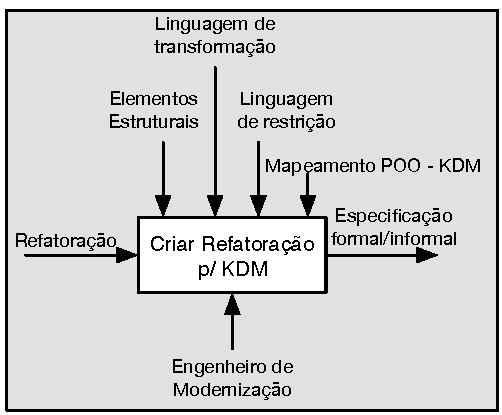
\includegraphics[scale=0.9]{images/criar_refatoracao_kdm}
	\fautor
\end{figure}


Na Figura~\ref{fig:todos_os_passos_diretrizes} uma micro-visão da Figura~\ref{fig:diretrizes_kdm_refatoracao_capitulo} é apresentada. Nota-se que a criação de refatorações para o metamodelo KDM possui cinco principais atividades que o engenheiro de modernização deve seguir. Nas subseções a seguir essas atividades são apresentadas. %Gerenciamento de consistência e Apoio computacional são apresentados no Capítulo~\ref{chapter:Abordagem_de_sincronizacao} e Capítulo~\ref{chapter:ferramenta_kdm_re}, respectivamente.


\begin{figure}[h]
	\centering
	% Requires \usepackage{graphicx}
	\caption{Diretrizes para criar refatorações para o KDM.}
	\label{fig:todos_os_passos_diretrizes}
	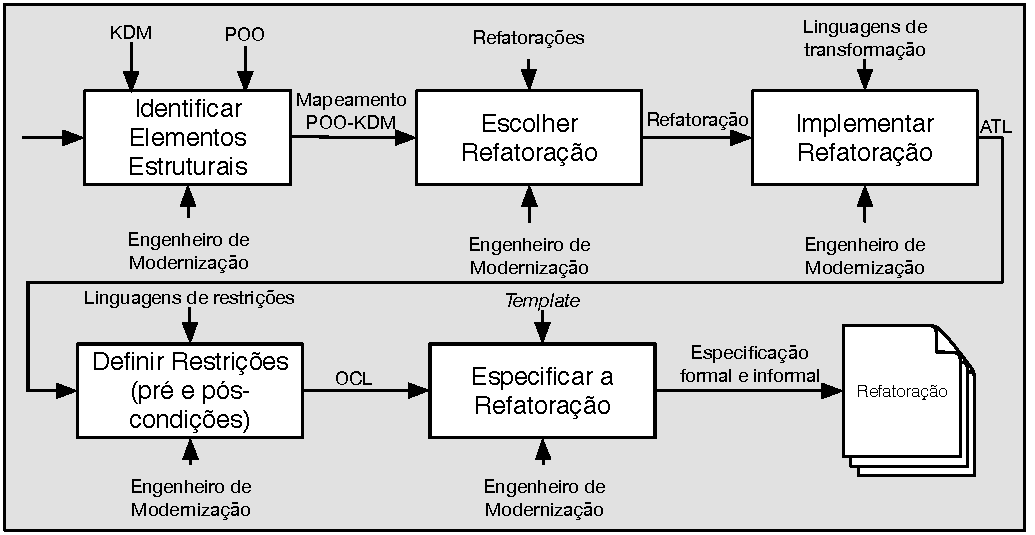
\includegraphics[scale=0.9]{images/fasesParaConstruirRefatoracoesKDM2}
	\fautor
\end{figure}

\subsection{Identificar Elementos Estruturais}\label{sec:mapeamento_POO_e_KDM}

Nesta atividade o objetivo é traduzir os conceitos do POO para o metamodelo KDM. É identificado os elementos estruturais do POO em relação as metaclasses disponíveis no metamodelo KDM. De acordo com~\citeonline{Zhang_2005, Boger_2003} um dos maiores desafios quando necessita-se adaptar refatorações para um determinado metamodelo é saber quais são as metaclasses corretas que representam determinadas construções/declarações de um determinado paradigma de programação. É importante identificar se a metaclasse escolhida para fazer a refatoração representa realmente o elemento e o conceito do POO. Dessa forma, antes de realizar a adaptação de qualquer refatoração para o metamodelo KDM, deve-se primeiramente identificar as metaclasses do KDM que têm características similares aos conceitos do POO, bem como instruções comumente utilizadas em todas as linguagens de programação, tais como, ramificações, iterações, etc. 

Um mapeamento entre os conceitos/elementos do POO e as metaclasses do metamodelo KDM foi realizado. Esse mapeamento pode ser visto na Tabela~\ref{tab:mapemanetoEntreOOPeKDM}. Nessa tabela é possível visualizar as metaclasses do metamodelo KDM que possuem características similares aos conceitos/elementos do POO. Utilizando essa Tabela~\ref{tab:mapemanetoEntreOOPeKDM}, engenheiros de modernização podem identificar os elementos estruturais necessários para adaptar as refatorações para o metamodelo KDM. Assim, qualquer exemplo de refatoração definida para o POO pode ser adaptada para o metamodelo KDM. Como observado, a Tabela~\ref{tab:mapemanetoEntreOOPeKDM} contêm três colunas: \aspas{Elemento do Código-fonte}, \aspas{Pacote::metaclasse do KDM} e \aspas{Descrição}. A primeira coluna informa a construção da linguagem de programação (\textit{statement})e/ou o conceito e do POO (pacote, classe, interface, etc), respectivamente. Em seguida a coluna \aspas{Pacote::metaclasse do KDM} apresenta a metaclasse responsável por mapear a construção e/ou o conceito do POO. Note que essa coluna segue o formato \aspas{Package::Meta-class}. A ultima coluna, \aspas{Descrição}, contêm informações sobre a metaclasse, tais como: seu propósito, seus meta-atributos e suas meta-associações.

\begin{longtable}[c]{| m{1.9cm} | m{3.57cm}| m{9.3cm} |}
 \caption{Mapeamento entre POO e metaclasses do metamodelo KDM.\label{tab:mapemanetoEntreOOPeKDM}}\\
 
 \hline
 \multicolumn{3}{| c |}{Início da Tabela}\\
 \hline
 Elemento do Código-Fonte & Pacote::metaclasse do KDM & Descrição\\
 \hline
 \endfirsthead
 
 \hline
 \multicolumn{3}{|c|}{Continuação da Tabela~\ref{tab:mapemanetoEntreOOPeKDM}}\\
 \hline
 Elemento do Código-Fonte & Pacote::metaclasse do KDM & Descrição\\
 \hline
 \endhead
 
 \hline
 \endfoot
 
 \hline
 \multicolumn{3}{| c |}{Fim da Tabela~\ref{tab:mapemanetoEntreOOPeKDM}}\\
 \hline\hline
 \endlastfoot
 
 Pacote & code::Package & A metaclasse \texttt{Package} é um contêiner para elementos de programa, como classes e interfaces. Essa metaclasse contêm um principal meta-atributo, \texttt{name}, que especifica o nome do pacote. Além disso, esta metaclasse contêm uma principal meta-associação \texttt{codeElement:AbstractCodeElement[0..*]} onde, pacotes, classes e interfaces podem ser incluídos. \\ 
\hline
Classe & code::ClassUnit & A metaclasse \texttt{ClassUnit} possui dois principais meta-atributos,  \texttt{name:String} e \texttt{isAbstract:boolean}. O primeiro é utilizado para especificar o nome da classe, o segundo é utilizado para informar se a classe é ou não abstrata. Além disso, essa metaclasse possui três meta-associações: \texttt{attribute:Attribute[0..*]}, \texttt{codeRelation:KDMRelationship[0..*]} e  \texttt{codeElement:AbstractCodeElement[0..*]}. \texttt{attribute} é utilizado para especificar a  visibilidade da classe, ou seja, \textit{public}, \textit{private}, ou \textit{protected}. \texttt{codeRelation} agrupa todos os relacionamentos que uma determinada classe contêm, por exemplo, heranças e associações. \texttt{codeElement} agrupa qualquer metaclasse cujo tipo é uma concretização de \texttt{AbstractCodeElement}, como: \texttt{StorableUnit}, \texttt{MethodUnit}, \texttt{MemberUnit}, etc. \\ 
\hline
Interface & code::InterfaceUnit & A metaclasse \texttt{InterfaceUnit} possui características similares a metaclasse \texttt{ClassUnit}, porém, não tem o meta-atributo \texttt{isAbstract}, uma vez que todas as interfaces são abstratas por padrão. \\ 
\hline
Atributo & code::StorableUnit & A metaclasse \texttt{StorableUnit} possui dois principais meta-atributos: \texttt{name:String} e \texttt{kind:StorableKind}. Similarmente, esse metaclasse possui duas principais meta-relacionamentos: \texttt{attribute:Attribute[..*]} e \texttt{type:DataType[1]}. \texttt{name} é utilizado para especificar o nome do atributo. \texttt{kind} é uma enumeração utilizada para especificar propriedades do atributo, ou seja, informar se o mesmo é local, global, estático, etc. \texttt{attribute} é utilizado para definir o escopo do atributo, \textit{public}, \textit{private}, ou \textit{protected}. E \texttt{type} é utilizado para definir o tipo do atributo.  \\ 
\hline
Método & code::MethodUnit & A metaclasse \texttt{MethodUnit} possui dois principais meta-atributos: \texttt{name:String} e \texttt{kind:MethodKind}. \texttt{name} é utilizado para especificar o nome do método. \texttt{kind} é uma enumeração utilizada para especificar propriedades do método, ou seja, informar se o método é \textit{construtor}, \textit{destructor}, \textit{virtual}, \textit{abstract}, etc. Similarmente, esse metaclasse possui dois principais meta-relacionamentos: \texttt{attribute:Attribute[..*]}, \texttt{codeElement:AbstractCodeElement[0..*]}. \texttt{attribute} é utilizado para definir o escopo do método - informar se o mesmo é \textit{public}, \textit{private}, ou \textit{protected}. E \texttt{codeElement} é utilizado para agrupar declarações internas do método, ou seja, assinatura do método, bloco do método, etc.\\ 
\hline
Assinatura do Método & code::Signature & A metaclasse \texttt{Signature} possui um principal meta-atributo, \texttt{name:String}, o qual é utilizado para especificar o nome do método. Além disso, essa metaclasse contêm um principal meta-relacionamento denominado \texttt{parameterUnit:ParameterUnit[..*]} que é utilizado para especificar os parâmetros que o método contêm.\\ 
\hline
Bloco do Método & action::BlockUnit & A metaclasse \texttt{BlockUnit} representa blocos lógicos e físicos relacionados, por exemplo, blocos de instruções \textit{if}, \textit{for}, \textit{while}, etc. Possui um meta-relacionamento denominado \texttt{codeElement:AbstractCodeElement[0..*]} que é utilizado para agrupar qualquer instruções lógicas ou físicas.\\ 
\hline
Parâmetro & code::ParameterUnit & A metaclasse \texttt{ParameterUnit} pode representar o nome, tipo e a posição dos parâmetros em uma assinatura de método. além de permitir o tipo de parâmetro (valor ou referência). Essa metaclasse contêm dois principais meta-atributos: \texttt{name:String} e \texttt{kind:ParameterKind}. O primeiro meta-atributo representa o nome do parâmetro, o segundo meta-atributo é uma enumeração para especificar o tipo de parâmetro (valor ou referência). Além disso, \texttt{ParameterUnit} contêm o meta-relacionamento \texttt{type:DataType[1]} para especificar o tipo do parâmetro, esse tipo pode ser tipos primitivos ou outros tipos.\\ 
\hline
Associação & code::HasType & A metaclasse \texttt{HasType} representa relação semântica entre um elemento de dados e seu tipo. Essa meta-calsse contêm duas principais meta-relacionamentos: \texttt{from:CodeItem} e \texttt{to:DataType}.\\ 
\hline
Herança \texttt{extends} & code::Extends & A metaclasse \texttt{Extends} representa relação semântica de herança entre duas \texttt{ClassUnits} ou duas \texttt{InterfaceUnits}. Essa relação semântica é representada por dois meta-relacionamentos: \texttt{from:DataType} e \texttt{to:DataType}.\\ 
\hline
Herança \texttt{implements} & code::Implements & A metaclasse \texttt{Implements} representa relação semântica de herança entre uma \texttt{ClassUnit} e uma \texttt{InterfaceUnit}. Similarmente a metaclasse \texttt{Extends} a relação semântica é representada por dois meta-relacionamentos: \texttt{from:DataType} e \texttt{to:DataType}.\\ 
\hline
\textit{if}, \textit{for}, \textit{while}, etc & action::ActionElement & \texttt{ActionElement} representa instruções e declarações de uma determinada linguagem de programação, ou seja, pode ser utilizada para representar ramificações, iterações, etc. \texttt{ActionElement} possui um principal meta-atributo denominado \texttt{kind:String} que representa qual o tipo instrução que a metaclasse esta representando. Essa metaclasse possui dois meta-relacionamentos \texttt{codeElement:AbstractCodeElement[0..*]} e \texttt{actionRelation:ActionRelationship[0..*]}.\\ 
\hline
 \end{longtable}


Na Tabela~\ref{tab:mapemanetoEntreOOPeKDM} é possível ver a relação existente entre os conceitos do POO, bem como algumas instruções de linguagens de programação e as algumas metaclasses do metamodelo KDM. Para atender aos objetivos deste trabalho a Tabela~\ref{tab:mapemanetoEntreOOPeKDM} apresenta apenas as principais metaclasses do KDM que são utilizadas nas refatorações aqui adaptado, uma vez que seria inviável mapear todas as noventa metaclasses do metamodelo KDM.

Como apresentado na Tabela~\ref{tab:mapemanetoEntreOOPeKDM} algumas metaclasses podem ser diretamente mapeadas com elementos do POO, tais como: classes (\texttt{ClassUnit}), interfaces (\texttt{InterfaceUnit}), atributos (\texttt{StorableUnit}), métodos (\texttt{MethodUnit}), etc. Entretanto, como o KDM tem como objetivo ser um metamodelo independente de plataforma para representar de forma genérica todas as abstrações e paradigmas de programação, algumas construções de programação não possuem uma metaclasse particular. Por exemplo, iterações e ramificações em KDM são representadas utilizando a mesma metaclasse, \texttt{ActionElement}. Esse mapeamento ocorre pois o KDM define uma metaclasse genérica para especificar ramificações e iterações para preservar a independência de plataforma; seria inviável para o metamodelo definir específicas metaclasses para representar ramificações e iterações uma vez que cada linguagem de programação possui um determinada particularidade. Para que o mapeamento fique o mais genérico e independente de plataforma possível a metaclasse \texttt{ActionElement} utiliza o meta-atributo \texttt{kind}, o qual contêm os seguintes valores: \textit{variable declaration}, \textit{if}, \textit{for}, \textit{while}, etc.

Com a utilização da Tabela~\ref{tab:mapemanetoEntreOOPeKDM} o engenheiro de modernização pode agora escolher qual refatoração criar para o metamodelo KDM. É de suma importância identificar previamente qual elemento do metamodelo KDM será utilizado durante a refatoração para o engenheiro criar e implementar a refatoração como apresentado na Seção~\ref{sec:linguagemDeTransformacaoUtilizada}. Por exemplo, suponha que o engenheiro de modernização almeja criar a refatoração \texttt{Rename Method}. Dessa forma, utilizando a Tabela~\ref{tab:mapemanetoEntreOOPeKDM} pode-se observar qual é a metaclasse em KDM que representa métodos; métodos em KDM são representados por instâncias da metaclasse \texttt{MethodUnit}, assim, a refatoração torna-se \texttt{Rename MethodUnit}. Adicionalmente, por meio da Tabela~\ref{tab:mapemanetoEntreOOPeKDM} é possível identificar todos os relacionamentos que a metaclasse \texttt{MethodUnit} possui, os quais podem ser úteis durante a implementação da refatoração.


\subsection{Escolher Refatoração}\label{sec:refatoracao_para_o_metamodelo_kdm}

Após identificar todos os elementos estruturais e identificar o mapeamento entre POO e o metamodelo KDM, o próximo passo é escolher qual refatoração criar. Dessa forma, nesta seção algumas refatorações propostas por~\citeonline{Fowler1999} foram escolhidas para serem adaptadas para o contexto do metamodelo KDM. As refatorações propostas por~\citeonline{Fowler1999} foram escolhidas para serem adaptas para o contexto do metamodelo KDM uma vez que são bem conhecidas, básicas e de baixa granularidade. As refatorações adaptadas seguem a mesma convenção de nomenclatura definida por~\citeonline{Fowler1999}. Porém, os nomes de algumas refatorações foram alteradas para indicar o metamodelo KDM como seu novo domínio de aplicação, por exemplo, \texttt{MoveMethod} torna-se \texttt{MoveMethodUnit} e \texttt{MoveAttribute} torna-se \texttt{MoveStorableUnit}, etc. 

No contexto desta Tese todas as refatorações são transformações que são realizadas em uma instância do metamodelo KDM. Assim, as refatorações podem ser agrupadas em nível de sua granularidade. As granularidades podem ser definidas em dois níveis de operações: (\textit{i}) operações atômicas e (\textit{ii}) operações compostas. As granularidades definidas como operações atômicas podem ser especificadas por meio de operações primitivas que são executadas na instância do metamodelo KDM. Tais operações primitivas são listadas a seguir:

\begin{itemize}
\item \texttt{add}: qualquer operação que adicione uma instância de uma metaclasse do metamodelo KDM (ver Tabela~\ref{tab:mapemanetoEntreOOPeKDM});
\item \texttt{delete}: qualquer operação que remove uma instância de uma metaclasse do metamodelo KDM (ver Tabela~\ref{tab:mapemanetoEntreOOPeKDM});
\item \texttt{change}: qualquer operação que altere um valor de um meta-atributo de uma metaclasse do metamodelo KDM (ver Tabela~\ref{tab:mapemanetoEntreOOPeKDM}).
\end{itemize}

As refatorações de granularidade compostas consistem em uma combinação de operações atômicas. Por exemplo, considere a refatoração \texttt{MoveStorableUnit}, essa refatoração compõe-se de duas operações atômicas: \texttt{add} e \texttt{delete}. Na Tabela~\ref{tab:refatoringsCatalogo} as refatorações que podem ser facilmente criadas para o metamodelo KDM são apresentadas.

\begin{table}[h]
\caption{Refatorações adaptadas para o metamodelo KDM.\label{tab:refatoringsCatalogo}}
\begin{center}
\begin{tabular}{ | m{4.5cm} | m{2.5cm} | m{4cm}| } 
\hline
\multicolumn{1}{|c|}{Refatoração} & \multicolumn{1}{|c|}{Granularidade} & \multicolumn{1}{|c|}{Tipo de Operação}\\ 
\hline
\textit{Add Package} &  Atômica & \texttt{add}\\ 
\hline
\textit{Add ClassUnit} &  Atômica & \texttt{add}\\ 
\hline
\textit{Add StorableUnit} &  Atômica & \texttt{add}\\ 
\hline
\textit{Add MethodUnit} &  Atômica & \texttt{add}\\ 
\hline
\textit{Delete Package} &  Atômica & \texttt{delete}\\ 
\hline
\textit{Delete ClassUnit} &  Atômica & \texttt{delete}\\ 
\hline
\textit{Delete StorableUnit} &  Atômica & \texttt{delete}\\ 
\hline
\textit{Delete MethodUnit} &  Atômica & \texttt{delete}\\ 
\hline
\textit{Rename Package} &  Atômica & \texttt{Change}\\ 
\hline
\textit{Rename ClassUnit} &  Atômica & \texttt{Change}\\ 
\hline
\textit{Rename StorableUnit} &  Atômica & \texttt{Change}\\ 
\hline
\textit{Rename MethodUnit} &  Atômica & \texttt{Change}\\ 
\hline
\textit{Move StorableUnit} &  Composta & \texttt{add} $|$ \texttt{delete}\\ 
\hline
\textit{Move MethodUnit} &  Composta & \texttt{add} $|$ \texttt{delete}\\ 
\hline
\textit{Extract ClassUnit} &  Composta & \texttt{add} $|$ \texttt{delete} $|$ \texttt{change}\\
\hline
\textit{Inline ClassUnit} &  Composta & \texttt{change} $|$ \texttt{delete}\\ 
\hline
\textit{Flatten Hierarchy} &  Composta & \texttt{add} $|$ \texttt{delete} $|$ \texttt{change}\\ 
\hline
\textit{Push Down MethodUnit} &  Composta & \texttt{add} $|$ \texttt{delete}\\ 
\hline
\textit{Push Down StorableUnit} &  Composta & \texttt{add} $|$ \texttt{delete}\\ 
\hline
\textit{Pull Up MethodUnit} &  Composta & \texttt{add} $|$ \texttt{delete}\\
\hline
\textit{Pull Up StorableUnit} &  Composta & \texttt{add} $|$ \texttt{delete}\\
\hline
\textit{Extract SubClass} &  Composta & \texttt{add} $|$ \texttt{change}\\
\hline
\textit{Encapsulate StorableUnit} &  Composta & \texttt{add} $|$ \texttt{change}\\
\hline
\end{tabular}
\end{center}
\end{table}

Após definidar qual refatoração o engenheiro de modernização irá criar para o metamodelo KDM o próximo passo é implementar a refatoração utilizando técnicas e linguagem de transformação em modelo. Na próxima seção maiores informações são apresentadas.

\subsection{Implementar Refatoração}\label{sec:linguagemDeTransformacaoUtilizada}

Na literatura é possível identificar um conjunto de técnicas e linguagens específicas para auxiliar a condução e especificação de transformação de modelos~\cite{Biehl_2010, Mens_2006, Allilaire_06}. As duas abordagens mais utilizadas na literatura para a elaboração e condução de transformações/refatoração de modelos são: (\textit{i}) abordagem de manipulação direta e (\textit{ii}) abordagem de transformação genérica. A primeira abordagem utiliza linguagens de programação tradicional para a aplicação das refatorações. Ferramentas que utilizam essa abordagem utilizam linguagens como Java, C, C++ etc~\cite{Bruneliere_2014}. Usualmente tais linguagens proporcionam uma infraestrutura mínima para organizar as transformações. Algumas características de suma importância para refatorações de modelo como, regras de transformações, preservação de comportamento são, usualmente criadas pelo engenheiro, uma vez que tais linguagens não possuem API para lidar com tais características. Dessa forma, refatorações que utilizam essa abordagem tornam-se dependente de plataformas, afetando assim a reusabilidade das refatorações. 

A segunda abordagem, transformação genérica, utiliza linguagens desenvolvidas especialmente para realizar transformações em modelos, tais como ATL, QVT, Kermeta, etc. Usualmente, tais abordagens são conhecidas como endógenas e são implementadas utilizando técnicas de reescrita de grafo (ver Capítulo~\ref{chapter:fundamentacao_teorica} Seção~\ref{sec:transformacoes_de_modelos}). Diferentemente da primeira abordagem, a segunda abordagem facilita o reúso de refatorações. Por exemplo, utilizando a segunda abordagem o engenheiro de modernização pode criar um conjunto de regras de refatorações por meio de linguagens de transformações genéricas, assim, tais refatorações podem ser invocadas utilizando qualquer linguagem de programação. O engenheiro poderia escrever um código em Java que iria ter como entrada uma instância do metamodelo KDM para ser refatorado, a reforação a ser aplicada nessa instância e um conjunto de parâmetros para realizar a refatoração na instância do metamodelo KDM.

Dado essa motivação, no contexto desta Tese, a segunda abordagem é utilizada. Mais especificamente a linguagem de transformação ATL~\cite{ATL_eclipse,Jouault_2008} foi escolhida para definir e implementar refatorações em instâncias do metamodelo KDM. ATL foi escolhida como linguagem de transformação considerando vários aspectos. Essa linguagem está integrada na plataforma Eclipse, o que fornece uma série de recursos padrões para o desenvolvimento (\textit{syntax highlighting} e \textit{debugger}). ATL é parte do projeto \textit{Model-To-Model} e possui um grupo de discussão ativo, constantemente atualizado, vários exemplos e diversos estudos de casos aplicados até mesmo na indústria utilizam tais linguagens.


ATL possui um modulo de execução denominado \textit{refining} que é utilizado para criar refatorações em nível de modelo. Esse modulo foi introduzido para facilitar a programação de (ou refatoração) transformações. Com o modulo \textit{refining}, os engenheiros de modernização podem se concentrarem no código ATL dedicada à geração de elementos estruturados modificados. Outros elementos estruturados do KDM (por exemplo, aqueles que permanecem inalteradas antes e após a refatoração) são implicitamente processados pelo mecanismo de ATL. O modulo \textit{refining} pode ser utilizado simplesmente substituindo a palavra-chave \texttt{from} pela palavra-chave \texttt{refining}. Obviamente, o modo de \textit{refining} só pode ser utilizado para as transformações endógenas (\aspas{\textit{in-place}}) (ver Capítulo~\ref{chapter:fundamentacao_teorica}, Seção~\ref{sec:transformacoes_de_modelos})


Como apresentado na Seção~\ref{sec:refatoracao_para_o_metamodelo_kdm} as refatorações são agrupadas em dois níveis de operações: (\textit{i}) operações atômicas e (\textit{ii}) operações compostas. As granularidades definidas como operações atômicas são: \texttt{add}, \texttt{delete} e \texttt{change}. Essas operações atômicas podem ser facilmente implementadas em ATL. Por exemplo, no Código-fonte~\ref{codigo:exemplo_add_classUnit} apresentado é uma simples ATL que adiciona uma nova instância da metaclasse \texttt{ClassUnit} denominada \texttt{novaClassUnit} no pacote \texttt{com.br.teste}. Como pode ser observado na linha 5 é especificado o nome do pacote (\aspas{com.br.teste}) que a nova instância da \texttt{ClassUnit} será adicionada. A linha 8 representa que a nova instância da \texttt{ClassUnit} será adicionada no associação \texttt{codeElement}. Nas linhas 10-12 uma nova instância da metaclasse \texttt{ClassUnit} é adicionada e seu nome definido como \aspas{novaClassUnit}.

\begin{codigo}[caption={[ATL para realizar a operação atômica \textit{add} \texttt{ClassUnit}.] ATL para realizar a operação atômica \textit{add} \texttt{ClassUnit}.},escapeinside={(*@}{@*)}, basicstyle=\footnotesize, label={codigo:exemplo_add_classUnit}, language=ATL]{Name}
module addAClassUnit;
create OUT : MM refining IN : MM;
rule createAClass{
	from
		source : MM!Package (source.name = (*@\aspas{com.br.teste}@*))
	to 
		target: MM!Package (
			codeElement (*@$\leftarrow$@*) source.codeElement(*@$\rightarrow$@*)including(newClassUnit)
		),
		newClassUnit: MM!ClassUnit (
			name (*@$\leftarrow$@*) (*@\aspas{novaClassUnit}@*)
		)
}
\end{codigo}

Da mesma forma o engenheiro de modernização pode implementar a operação atômica \texttt{delete} facilmente como apresentado no Código-fonte~\ref{codigo:exemplo_delete_classUnit}. 
É importante observar que a  palavra-chave \texttt{drop} é utilizada em ATL para remover uma determinada instância. Dessa forma, o engenheiro de modernização deve primeiro especificar qual instância almeja-se deletar.  Assim, na linha 5 é informado o nome da instância da \texttt{ClassUnit} que almeja-se deletar. Em seguida, nas linhas 6-8 a instância especificada é deletada. 

\begin{codigo}[caption={[ATL para realizar a operação atômica \textit{delete} \texttt{ClassUnit}.] ATL para realizar a operação atômica \textit{delete} \texttt{ClassUnit}.},escapeinside={(*@}{@*)}, basicstyle=\footnotesize, label={codigo:exemplo_delete_classUnit}, language=ATL]{Name}
module removeClassUnit;
create OUT : MM refining IN : MM;
rule deleteClassUnit {
  from
      source : MM!ClassUnit (source.name = (*@\aspas{ClassToRemove}@*))
  to
      drop
}
\end{codigo}

A última operação atômica é a operação \texttt{change}. Essa operação é responsável por alterar o valor de um meta-atributo de uma metaclasse do metamodelo KDM, como por exemplo \textit{Rename Package} apresentado no Código-fonte~\ref{codigo:exemplo_rename_Package}. Na linha 5 é especificado e identificado a instância da metaclasse \texttt{Package} que será alterada. Nas linhas 7-9 a instância especificada da metaclasse \texttt{Package} é alterada.

\begin{codigo}[caption={[ATL para realizar a operação atômica \textit{change} \texttt{ClassUnit}.] ATL para realizar a operação atômica \textit{change} \texttt{ClassUnit}.},escapeinside={(*@}{@*)}, basicstyle=\footnotesize, label={codigo:exemplo_rename_Package}, language=ATL]{Name}
module renamePackage;
create OUT : MM refining IN : MM;
rule rename {
	from
		source : MM!Package (source.name=(*@\aspas{PackageToRename}@*))
	to 
		target : MM!Package (
			name (*@$\leftarrow$@*) (*@\aspas{newName}@*)
		)
}
\end{codigo}


Como apresentado na Tabela~\ref{tab:refatoringsCatalogo} com a combinação dessas operações atômicas os engenheiros de modernização podem criar refatorações mais significativas. O Código-fonte~\ref{codigo:exemplo_add_classUnit} e o Código-fonte~\ref{codigo:exemplo_delete_classUnit} ilustram as operações atômicas \texttt{add} e \texttt{delete} para instâncias da metaclasse \texttt{ClassUnit}, respectivamente. Porém, engenheiros de modernização podem adaptarem esses códigos para utilizam outros elementos estruturais tais como: \texttt{InterfaceUnit}, \texttt{StorableUnit}, \texttt{MethodUnit}, etc. Por exemplo, caso almeja-se deletar uma determinada instância da metaclasse \texttt{InterfaceUnit} o engenheiro de modernização deve apenas substituir a linha 5 do Código-fonte~\ref{codigo:exemplo_delete_classUnit} por \aspas{\texttt{source: MM!InterfaceUnit(source.name = \aspas{InterfaceToRemove})}}. 

Após a criação de uma refatoração o engenheiro de modernização deve especificar as restrições da refatoração criada. Tais restrições são especificadas utilizando linguagens de restrições como por exemplo OCL. Na próximo seção maiores informações são apresentadas.

\subsection{Definir Restrições (Pré- e Pós-condições)}\label{sec:linguagem_de_restricao}

Após o engenheiro de modernização criar uma determinada refatoração o próximo passo é criar restrições (pré- e pós-condições) para a refatoração. Usualmente antes e após a aplicação de uma determinada refatoração algumas restrições precisam ser satisfeitas. Tais restrições usualmente são úteis para verificar se os parâmetros necessários para executar a refatoração foi completamente e corretamente informando, bem como verificar se a refatoração foi aplicada de forma totalmente correta. No contexto de modelos, tais restrições são especificadas utilizando linguagem como OCL. Tais restrições no contexto de refatorações são conhecidas como pré- e pós-condições. Utilizando OCL, é possível verificar, por exemplo, se todos os parâmetros obrigatórios para executar o mecanismo da refatoração foram especificados pelo modernizador. Além disso, essas condições são importantes para assegurar que a refatoração será aplicada de forma correta e ainda irá preservar a semântica da instância do meta-modelo, como por exemplo, preservar comportamentos, sincronização, etc. 

Dessa forma, cada refatoração definida nesta Tese está associada com uma pré- e pós-condição definida em OCL. OCL foi escolhida pois a mesma é uma linguagem padronizada pela OMG e também possui suporte na plataforma Eclipse. É importante observar que as diretrizes apresentadas neste capítulo não têm a preocupação de ensinar como escrever/implementar as restrições das refatorações utilizando OCL. Assim, o engenheiro de modernização é responsável por criar e implementar todas as pré- e pós-condições de uma dada refatoração para o KDM.



%Com o intuito de facilitar a visualização, formalização e entendimento das refatorações criadas para o metamodelo KDM, as refatorações aqui apresentadas utilizam duas especificações~\cite{staron2004implementing}: (\textit{i}) especificação informal e (\textit{ii}) especificação formal. Na especificação informal a ideologia da reforação é expressada, usualmente essa ideologia é definida por meio de linguagem natural. A especificação formal é responsável por representar as pré- e pós-condições, bem como a transformação/refatoração em OCL e ATL, respectivamente. Acredita-se que ambas especificações são úteis para o engenheiro de modernização - a especificação informal é utilizada para facilitar a compreensão e o propósito da refatoração, enquanto que a especificação formal facilita a implementação da refatoração. Além disso, a especificação formal é de extrema importância para facilitar a automação das refatorações. Maiores detalhes sobre essas especificações são apresentados na Subseção~\ref{sec:template_refatoracao}.

\subsection{\textit{Template} de Definição de Refatoração para o metamodelo KDM}\label{sec:template_refatoracao}

Após definir a refatoração, sua implementação, bem como suas pré- e pós-condições para o metamodelo KDM é importante documentar a refatoração criada. Dessa forma, para facilitar a visualização, formalização e entendimento das refatorações criadas para o metamodelo KDM, os engenheiros de modernização devem especificar as refatorações criadas seguindo duas especificações~\cite{staron2004implementing}: (\textit{i}) especificação informal e (\textit{ii}) especificação formal. 

Na especificação informal a ideologia da reforação é expressada, usualmente essa ideologia é definida por meio de linguagem natural. A especificação formal é responsável por representar as pré- e pós-condições, bem como a transformação/refatoração em OCL e ATL, respectivamente. Acredita-se que ambas especificações são úteis para o engenheiro de modernização - a especificação informal é utilizada para facilitar a compreensão e o propósito da refatoração, enquanto que a especificação formal facilita a implementação da refatoração. Além disso, a especificação formal é de extrema importância para facilitar a automação das refatorações. Maiores detalhes sobre essas especificações são apresentados na Subseção~\ref{sec:template_refatoracao}.



%Dado a Definição~\ref{def:refatoracao} de refatoração no contexto desta Tese é importante apresentar como cada refatoração é especificada. Como já salientado, as refatorações são definidas utilizando duas especificações, informal e formal. Assim, 

As refatorações para o metamodelo KDM devem ser especificadas utilizando o seguinte \textit{template}:

\begin{enumerate}
	\item Especificação Informal:
		\begin{enumerate}
			\item Nome: o nome da refatoração;
			\item Definição: uma lista contendo os parâmetros utilizados na refatoração - após a definição dos parâmetros, eles são utilizados e referenciados dentro das especificações formal e informal por meio de \{...\};
			\item Objetivo: o objetivo da refatoração;
			\item Descrição (opcional): uma pequena explicação da refatoração;
			\item Pré-condição: uma lista de asserção que tem que ser verdade antes de realizar a refatoração;
			\item Pós-condição: uma lista de asserção que tem que ser verdade após a realização da refatoração;
			\item Mecanismo: uma mecanismo de transformação descrevendo todos os passos da refatoração, seguido de uma imagem ilustrando o antes e depois da aplicação da refatoração;
			\item Algoritmo: um algoritmo que descreve a refatoração.
		\end{enumerate}
	\item Especificação Formal:
		\begin{enumerate}
			\item Pré-condição: a pré-condição expressa em OCL;
			\item Algoritmo: a refatoração (\textit{model transformation}) definida em ATL;
			\item Pós-condição: a pós-condição expressa em OCL.
		\end{enumerate}
\end{enumerate}


\section{Catálogo de Refatoração para o metamodelo KDM}\label{sec:catalogo_refatoracao_kdm}

Para facilitar o entendimento de como as refatorações são criadas para o metamodelo KDM, nesta seção são apresentadas algumas refatorações que foram criadas para o KDM seguindo as atividades descritas anteriormente. As refatorações que foram criadas para o metamodelo KDM podem ser visualizadas na Tabela~\ref{tab:refatoringsCatalogo}. Porém, nesse capítulo apenas algumas refatorações são detalhadas. As refatorações aqui apresentadas bem como outras refatorações foram implementadas em um ambiente computacional denominado KDM-RE apresentado no Capítulo~\ref{chapter:ferramenta_kdm_re}. Nas próximas seções as refatorações \textit{Rename ClassUnit}, \textit{Push Down StorableUnit} e \textit{Extract ClassUnit} são apresentadas e detalhadas. Todas as refatorações são definidas programaticamente utilizando a linguagem de transformação ATL. A linguagem de restrição utilizada nas refatorações foi a OCL. Todas as refatorações aqui criadas são especificadas utilizando o \textit{template} apresentado anteriormente.



\subsection{Refatoração \textit{Rename ClassUnit}}
Nesta seção a refatoração \textit{Rename ClassUnit} é apresentada. Essa refatoração usualmente é aplicada quando o nome da classe não revela o seu real propósito~\cite{Fowler1999}. Assim, deve-se renomear a classe para um nome mais significativo. Note que a descrição da refatoração \textit{Rename ClassUnit} segue as atividades definidas, bem como o \textit{template} especificado anteriormente, primeiro a especificação informal da refatoração apresentada seguida da especificação formal.

\begin{enumerate}
	\item Especificação Informal:
		\begin{enumerate}
			\item Nome: \textit{Rename ClassUnit};
			\item Definição:
			    \begin{itemize}
			        \item \texttt{ClassUnit}Selecionada - uma classe que será renomeada;
			        \item novoNome - um novo nome para a \{\texttt{ClassUnit}Selecionada\}.
			    \end{itemize}
			\item Objetivo: Mudar o nome de uma \{\texttt{ClassUnit}Selecionada\} para \{novoNome\};
			\item Descrição (opcional): O nome atual da \{\texttt{ClassUnit}Selecionada\} não reflete seu propósito.
			\item Pré-condição:
			    \begin{itemize}
			        \item o \{novoNome\} segue convenções válidas para nomes de classes;
			        \item não existe outra \texttt{ClassUnit} com o mesmo nome dentro do mesmo \texttt{Package};
			        \item a \{\texttt{ClassUnit}Selecionada\} não deve conter nenhuma operação com o mesmo nome, ou seja, o \{novoNome\} não deve coincidir com outros métodos, construtor, etc. 
			    \end{itemize}
			\item Pós-condição:
			    \begin{itemize}
			        \item o nome da \{\texttt{ClassUnit}Selecionada\} é \{novoNome\};
			        \item todas as referencias para \{\texttt{ClassUnit}Selecionada\} são por meio do \{novoNome\};
			        \item todos os construtores da \{\texttt{ClassUnit}Selecionada\} são agora \{novoNome\}.
			    \end{itemize}
			\item Mecanismo: O primeiro passo no mecanismo da refatoração \textit{Rename ClassUnit} é mudar o meta-atributo \texttt{name} da \{\texttt{ClassUnit}Selecionada\} para \{novoNome\}. Porém, note na Figura~\ref{fig:antes_e_depois_rename_classUnit} \ding{202}, a qual representa uma instância simplificada do KDM, que antes de realizar a refatoração, tanto a \{\texttt{ClassUnit}Selecionada\} quanto seu construtor possuem o mesmo nome. Assim, como apresentado na Figura~\ref{fig:antes_e_depois_rename_classUnit} \ding{203} ambas instâncias devem ser atualizadas, ou seja, a \{\texttt{ClassUnit}Selecionada\} e o construtor devem mudar para \{novoNome\}. Similarmente, deve-se também mudar todas as chamadas para \{novoNome\}, isso é realizado por meio das metaclasses \texttt{Calls}, \texttt{Creates}, etc, no meta-relacionamento \texttt{to}. Note na Figura~\ref{fig:antes_e_depois_rename_classUnit_create} \ding{204} que a instância da metaclasse \texttt{Creates} contêm o meta-relacionamento \texttt{to} ainda com o nome antigo, assim, deve-se alterar para \{novoNome\} como apresentado na Figura~\ref{fig:antes_e_depois_rename_classUnit_create} \ding{205}.
			\begin{minipage}{.90\textwidth}
	\vspace*{\fill}
  \centering
	% Requires \usepackage{graphicx}
	\captionof{figure}{instância simplificada do KDM antes e depois da refatoração \textit{Rename ClassUnit}}
	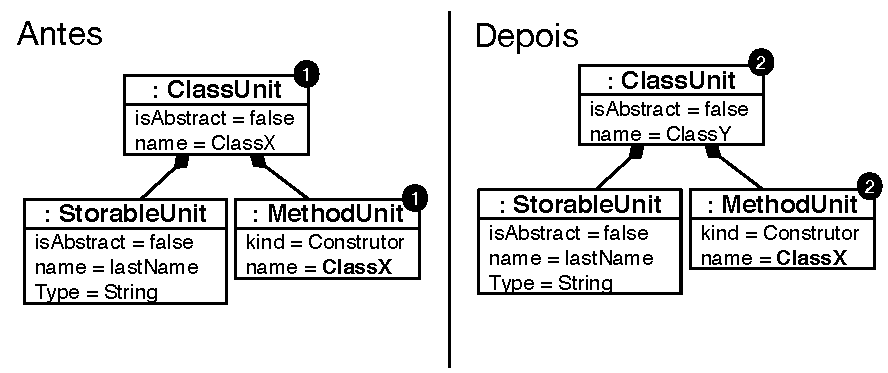
\includegraphics[scale=0.6]{images/antes_e_depois_rename_classUnit.pdf}
	\fautor
	\label{fig:antes_e_depois_rename_classUnit}
	\captionof{figure}{instância simplificada do KDM antes e depois da refatoração \textit{Rename ClassUnit} - parte 2}
	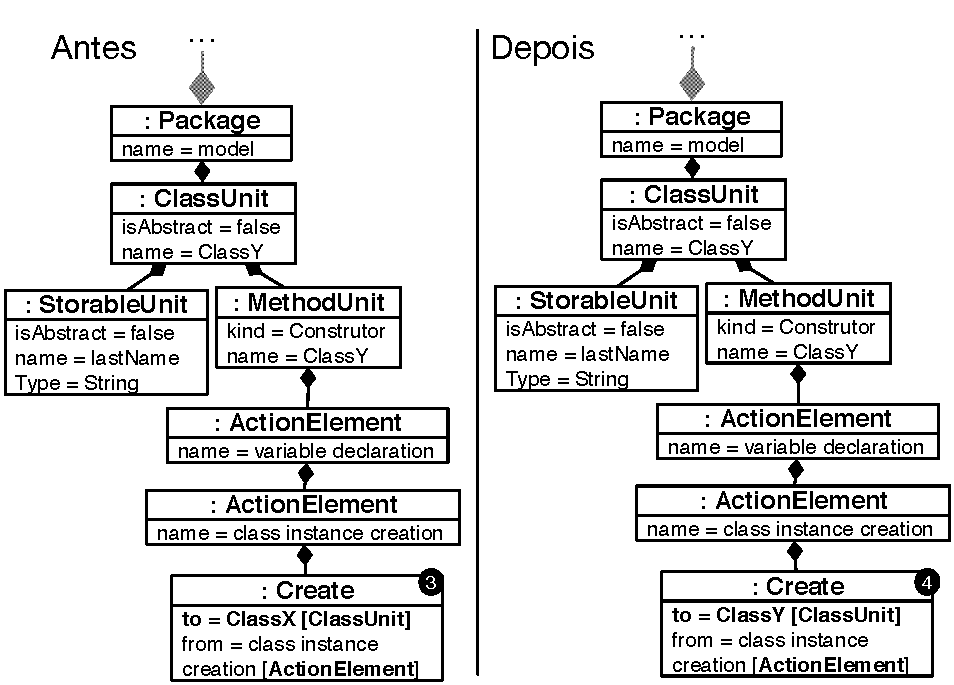
\includegraphics[scale=0.6]{images/antes_e_depois_rename_classUnit_Create.pdf}
	\fautor
	\label{fig:antes_e_depois_rename_classUnit_create}
\end{minipage}\hfill
			\item Algoritmo: 
			    \begin{itemize}
			        \item \{\texttt{ClassUnit}Selecionada\}.renameClassUnit(\{novoNome\});
			        \item para cada construtor - \texttt{MethodUnit.Kind=Construtor}.renameMethodUnit(\{novoNome\});
			        \item para cada referência da \{\texttt{ClassUnit}Selecionada\} deve-se mudar o meta-relacionamento \texttt{to} das metaclasses \texttt{Calls}, \texttt{Creates}, etc. 
			    \end{itemize}
		\end{enumerate}
	\item Especificação Formal:
		\begin{enumerate}
			\item Pré-condição: 
			\begin{codigo}[caption={[OCL representando a pré-condição da refatoração \textit{Rename ClassUnit}.] Pré-condição da refatoração \textit{Rename ClassUnit}.},escapeinside={(*@}{@*)}, basicstyle=\footnotesize, label={codigo:pre_renameClassUnit}, language=OCL]{Name}
context ClassUnit::preRenameClassUnit(newName: String)
pre : newName.isValidadName() 
and not ClassUnit.eContainer.codeElement(*@$\rightarrow$@*)exist (c : ClassUnit | c.name = newName) 
and not ClassUnit.codeElement(*@$\rightarrow$@*)exist (m: MethodUnit | m.name = newName and m.kind =  method)
\end{codigo}

%É importante observar que deve-se especificar a \texttt{ClassUnit} que será renomeada, bem como definir o novo nome dessa \texttt{ClassUnit} antes de executar a pré-condição, como apresentado no Código-fonte~\ref{codigo:pre_renameClassUnit}. 
Na linha 1 do Código-fonte~\ref{codigo:pre_renameClassUnit} é declarado o nome da pré-condição, também é declarado que essa restrição, é apenas executada para instâncias da metaclasse \texttt{ClassUnit}. Na linha 2 verifica-se se o parâmetro \texttt{newName} é um nome válido. Posteriormente, na linha 3 é verificado também se existe outra instância de \texttt{ClassUnit} com o mesmo valor do parâmetro \texttt{newName}. Linha 4 é verificado se existe alguma instância de \texttt{MethodUnit} com o mesmo valor do parâmetro \texttt{newName}. Caso a restrição definida na pré-condição seja válida a refatoração \textit{Rename ClassUnit} é executada.
			\item Algoritmo: 
	\begin{codigo}[caption={[ATL representando a refatoração \textit{Rename ClassUnit}.] ATL da refatoração \textit{Rename ClassUnit}.},escapeinside={(*@}{@*)}, basicstyle=\footnotesize, label={codigo:rename_classUnit_refatoracao}, language=ATL]{Name}
module renameClassUnit;
create OUT : MM refining IN : MM;
rule renameClassUnit {
	from
		source : MM!ClassUnit (source.name = (*@\aspas{\{\texttt{ClassUnit}Selecionada\}}@*))
	to 
		target : MM!ClassUnit (
			name (*@$\leftarrow$@*) (*@\aspas{newName}@*)
		)
}
rule renameConstrutor {
	from
		source : MM!MethodUnit (source.name = (*@\aspas{\{\texttt{ClassUnit}Selecionada\}}@*) and source.kind=(*@\aspas{constructor}@*))
	to 
		target : MM!MethodUnit (
			name (*@$\leftarrow$@*) (*@\aspas{newName}@*)
		)
}
\end{codigo}
			Como pode ser observado no Código-fonte~\ref{codigo:rename_classUnit_refatoracao} na linha 1 primeiramente é definido o nome da refatoração. Em seguida, na linha 2 é apresentado o cabeçalho da refatoração, note a palavra-chave \textit{refining}. Essa palavra-chave informa que essa transformação/refatoração é do tipo endógenas (\textit{in-place}) (ver Capítulo~\ref{chapter:fundamentacao_teorica} Seção~\ref{sec:transformacoes_de_modelos}), ou seja, irá alterar uma mesma instância do metamodelo KDM. Linha 3 até linha 10 a primeira regra é definida. Linha 5 uma condição de guarda é definida, a qual informa que apenas uma instância da metaclasse do tipo \texttt{ClassUnit} que possui um nome especifico será selecionada para a refatoração. Nas linhas 7, 8 e 9 o nome da instância da metaclasse do tipo \texttt{ClassUnit} é alterado. Posteriormente deve-se também alterar o nome do construtor, isso é realizado na regra especificado nas linha 11 até 17. Na linha 13 uma condição de guarda é especificada para informar que apenas métodos do tipo construtor devem ser obtidos, bem como o método deve possuir o mesmo nome da classe selecionada para aplicar a refatoração. Linhas 15, 16 e 17 o nome do construtor é alterado. Observe que tanto \{\texttt{ClassUnit}Selecionada\} quanto \{\textit{newName}\} são parâmetros que devem ser especificados pelo engenheiro. Assim, foi criado um \textit{plug-in} para auxiliar o engenheiro durante a especificação e execução das refatorações. Maiores informações sobre esse \textit{plug-in} estão no Capítulo X.     
			\item Pós-condição:
			 \begin{codigo}[caption={[OCL representando a pós-condição da refatoração \textit{Rename ClassUnit}.] Pós-condição da refatoração \textit{Rename ClassUnit}.},escapeinside={(*@}{@*)}, basicstyle=\footnotesize, label={codigo:pos_condicao_rename_classUnit}, language=OCL]{Name}
 context ClassUnit::RenameClassUnit(newName: String)
 post : name = newName and ClassUnit.eContainer.codeElement(*@$\rightarrow$@*)exist (m : MethodUnit | implies m.name = newName)
\end{codigo}
Na linha 1 do Código-fonte~\ref{codigo:pos_condicao_rename_classUnit} é declarado o nome da pós-condição, também é declarado que essa restrição, é apenas executada para o contexto de instâncias da metaclasse \texttt{ClassUnit}. Na linha 2 o parâmetro \texttt{newName} é comparado com o nome da \texttt{ClassUnit} refatorada, além disso, na linha 2 também é verificado se o construtor também foi alterado o seu nome corretamente. Se ambas as condições foram válidas, a refatoração foi realizada com sucesso.
		\end{enumerate}
\end{enumerate}
		
%--------------------------
\subsection{Refatoração \textit{Push Down StorableUnit}}
Nesta seção a refatoração \textit{Push Down StorableUnit} é apresentada. Essa refatoração é utilizada para remover a generalização de atributos, ou seja, um atributo é apenas utilizado em algumas sub-classes não em todas, assim, não é interessante manter a generalização do atributo na super-classe, uma vez que cada sub-classe pode definir um comportamento para o atributo~\cite{Fowler1999}.

\begin{enumerate}
	\item Especificação Informal:
		\begin{enumerate}
			\item Nome: \textit{Push Down StorableUnit};
			\item Definição:
			    \begin{itemize}
			        \item \texttt{StorableUnit}Selecionado - um atributo que será movido para sub-classes;
			        \item \texttt{ClassUnit} - uma classe na qual o \{\texttt{StorableUnit}Selecionado\} é definido;
			        \item sub-\texttt{ClassUnit}Selecionadas - sub-classes de \{\texttt{ClassUnit}\}.
			    \end{itemize}
			\item Objetivo: Mover um \{\texttt{StorableUnit}Selecionado\} para as \{sub-\texttt{ClassUnit}Selecionadas\}.
			\item Descrição (opcional): \{\texttt{StorableUnit}Selecionado\} é utilizada em apenas algumas sub-classes.
			\item Pré-condição:
			    \begin{itemize}
			        \item \{\texttt{StorableUnit}Selecionado\} não é utilizado em \texttt{ClassUnit};
			        \item as sub-\texttt{ClassUnit}Selecionadas não contêm as mesmas características do \{\texttt{StorableUnit} Selecionado\}, ou seja, os nomes e tipos são diferentes.
			    \end{itemize}
			\item Pós-condição:
			    \begin{itemize}
			        \item \{\texttt{StorableUnit}Selecionado\} não é definido em \texttt{ClassUnit};
			        \item todos os \textit{siblings} de \{\texttt{StorableUnit}Selecionado\} estão definidos nas sub-\texttt{ClassUnit}Selecionadas.
			    \end{itemize}
			\item Mecanismo: Na Figura~\ref{fig:antes_e_depois_pushDown_StorableUnit} duas instâncias simplificada do KDM são ilustradas, a parte superior ilustra a instância antes da realização da refatoração \textit{Push Down StorableUnit} e a parte inferior representa o resultado da refatoração. Como observado, o primeiro passo da refatoração \textit{Push Down StorableUnit} é selecionar um específico \texttt{StorableUnit}, Figura~\ref{fig:antes_e_depois_pushDown_StorableUnit} \ding{202}. Em seguida, deve-se selecionar as sub-classes que realmente utilizam esse \texttt{StorableUnit} para move-lo, com ilustrado na Figura~\ref{fig:antes_e_depois_pushDown_StorableUnit} \ding{203}. Posteriormente o \{\texttt{StorableUnit}Selecionado\} é movido para as sub-\texttt{ClassUnit}Selecionadas, como ilustrado na parte inferior da Figura~\ref{fig:antes_e_depois_pushDown_StorableUnit} \ding{205}. Note que a instância da \texttt{ClassUnit} que havia o \{\texttt{StorableUnit}Selecionado\} não possui mais sua instância, como apresentado na Figura~\ref{fig:antes_e_depois_pushDown_StorableUnit} \ding{204}.
			
			
\begin{minipage}{.90\textwidth}
	\vspace*{\fill}
  \centering
	% Requires \usepackage{graphicx}
	\captionof{figure}{Instância simplificada do KDM antes e depois da refatoração \textit{Push Down StorableUnit}}
	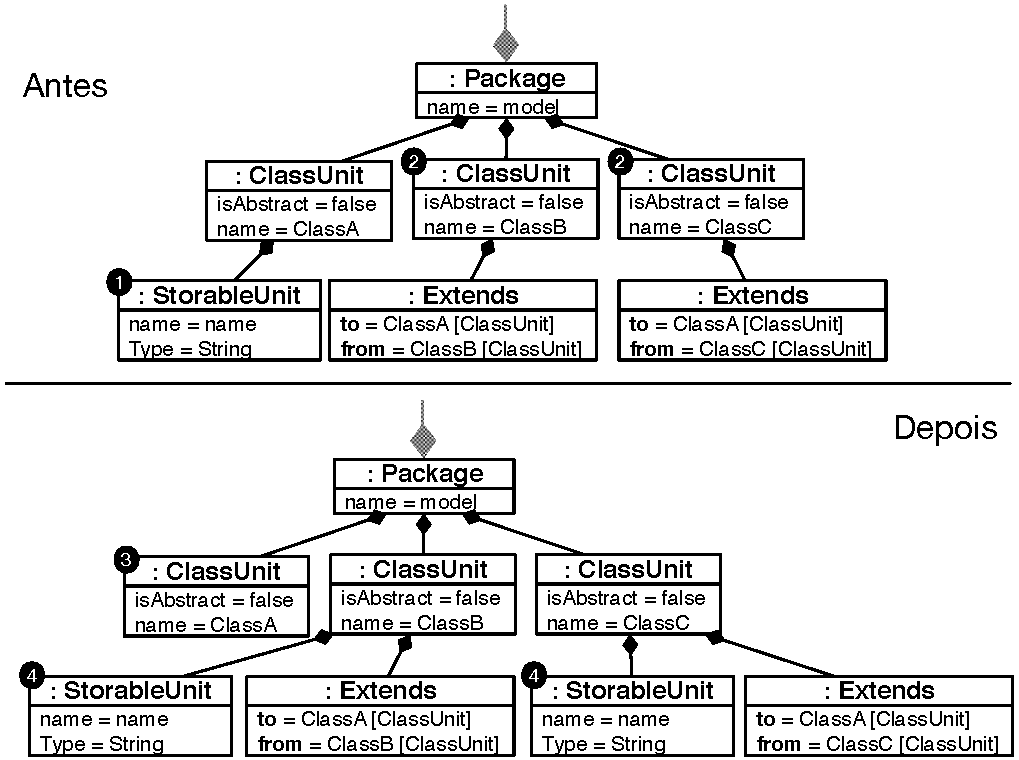
\includegraphics[scale=0.6]{images/antes_e_depois_push_down_storableUnit.pdf}
	\fautor
	\label{fig:antes_e_depois_pushDown_StorableUnit}
\end{minipage}\hfill
			\item Algoritmo: 
			    \begin{itemize}
			        \item para cada sub-\texttt{ClassUnit}Selecionadas que realmente usa o \{\texttt{StorableUnit}Selecionado\} - sub-\texttt{ClassUnit}Selecionadas.add(\{\texttt{StorableUnit}Selecionado\})
			        \item \{\texttt{ClassUnit}\}.remove(\{\texttt{StorableUnit}Selecionado\}). 
			    \end{itemize} 
	    \end{enumerate}
		\item Especificação Formal:
		\begin{enumerate}
			\item Pré-condição: 
			\begin{codigo}[caption={[OCL representando a pré-condição da refatoração \textit{Push Down StorableUnit}.] Pré-condição da refatoração \textit{Push Down StorableUnit}.},escapeinside={(*@}{@*)}, basicstyle=\footnotesize, label={codigo:pre_push_down_storableUnit}, language=OCL]{Name}
context StorableUnit::PushDownStorableUnit(subClasses:(ClassUnit))
pre : self.refImmediateComposite().codeElement(*@$\rightarrow$@*)forAll (m: MethodUnit |  not (m.codeRelation(*@$\rightarrow$@*)exists(r: Reads | r.to = self)) 
and not (m.codeRelation(*@$\rightarrow$@*)exists (w:Writes | w.to = self)) 
and not (m.codeRelation(*@$\rightarrow$@*)exists (a: Addresses | a.to = self) 
and subClasses(*@$\rightarrow$@*)forAll (c: ClassUnit | not c.codeElement(*@$\rightarrow$@*)exists(s: StorableUnit | s.name = self.name)))
\end{codigo}



%É importante observar que deve-se especificar a \texttt{ClassUnit} que será renomeada, bem como definir o novo nome dessa \texttt{ClassUnit} antes de executar a pré-condição, como apresentado no Código-fonte~\ref{codigo:pre_renameClassUnit}. 
Na linha 1 do Código-fonte~\ref{codigo:pre_push_down_storableUnit} é declarado a assinatura da pré-condição da refatoração \textit{Push Down StorableUnit}. Note que apenas é utilizado como parâmetro as sub-classes selecionadas para mover o \{\texttt{StorableUnit}Selecionado\}. Na linha 2 a instância da \texttt{ClassUnit} que contêm o \{\texttt{StorableUnit}Selecionado\} é obtida por meio da função \texttt{refImmediateComposite()}. Posteriormente, todas as instâncias de \texttt{MethodUnit} são obtidas para realizar uma iteração. Ainda na linha 2, essa iteração verifica se o \{\texttt{StorableUnit}Selecionado\} é lido em alguma instância de \texttt{MethodUnit}. Similarmente, na linha 3 e 4 todos os \texttt{MethodUnits} são verificados para identificar se o \{\texttt{StorableUnit}Selecionado\} é escrito e utilizado. Na linha 5 todas as \{sub-\texttt{ClassUnit}Selecionadas\} são verificadas para identificar se existe uma instância similar ao \{\texttt{StorableUnit}Selecionado\} antes de realizar a refatoração. Caso a pré-condição definida seja válida a refatoração \textit{Push Down StorableUnit} é executada.
			\item Algoritmo: 
	\begin{codigo}[caption={[ATL representando a refatoração \textit{Push Down StorableUnit}.] ATL da refatoração \textit{Push Down StorableUnit}.},escapeinside={(*@}{@*)}, basicstyle=\footnotesize, label={codigo:push_Down_StorableUnit_ATL}, language=ATL]{Name}
module pushDownStorableUnit;
create OUT : MM refining IN : MM;
rule pushDownStorableUnit {
	from
		source : MM!ClassUnit (source.name = (*@\aspas{\{sub-\texttt{ClassUnit}Selecionada\}}@*) or source.name = (*@\aspas{\{sub-\texttt{ClassUnit}Selecionada\}}@*))
	to 
		target : MM!ClassUnit (
			codeElement(*@$\leftarrow$@*)source.codeElement(*@$\rightarrow$@*)including(attr)
		),
		attr: MM!StorableUnit (
			name(*@$\leftarrow$@*)(*@\{\texttt{StorableUnit}Selecionado.name\}@*),
			type(*@$\leftarrow$@*)(*@\{\texttt{StorableUnit}Selecionado.type\}@*)
		)
}
rule removeStorableUnitFromSuperClass {
	from
		source : MM!StorableUnit (source.name = (*@\{\texttt{StorableUnit}Selecionado.name\}@*) and not source.refImmediateComposite().codeRelation.isEmpty())
	to
		drop
}
\end{codigo}
Na linha 1 do Código-fonte~\ref{codigo:push_Down_StorableUnit_ATL} o nome da refatoração é definido. Em seguida, na linha 2 é apresentado o cabeçalho da refatoração, novamente a palavra-chave \textit{refining} é especificada para informar que a transformação/refatoração é do tipo endógenas (ver Capítulo~\ref{chapter:fundamentacao_teorica} Seção~\ref{sec:transformacoes_de_modelos}). Posteriormente, nas linhas 3 até 13 a primeira regra dessa refatoração é definida. Na linha 5 uma condição de guarda é definida para identificar quais são as \{sub-\texttt{ClassUnit}Selecionadas\}. Em seguida, linhas 7, 8 e 9 informa que uma nova instância de \texttt{StorableUnit} será criado nas \{sub-\texttt{ClassUnit}Selecionadas\}. Nas linhas 10, 11 e 12 os meta-atributos do \{\texttt{StorableUnit}Selecionado\} são copiados. Após mover o \{\texttt{StorableUnit}Selecionado\} para as sub-classes, o próximo passo é remover o \{\texttt{StorableUnit}Selecionado\} da super-classe. Esse passo é representado na regra descrita nas linhas 15 até 20. Na linha 17 o \{\texttt{StorableUnit}Selecionado\} é identificado, depois na linha 19 a palavra-chave \textit{drop} é utilizada, a qual especifica que uma determinada instância será removida, neste caso o \{\texttt{StorableUnit}Selecionado\}.   
			\item Pós-condição:
			 \begin{codigo}[caption={[OCL representando a pós-condição da refatoração \textit{Push Down StorableUnit}.] Pós-condição da refatoração \textit{Push Down StorableUnit}.},escapeinside={(*@}{@*)}, basicstyle=\footnotesize, label={codigo:pos_condicao_pushDown_StorableUnit}, language=OCL]{Name}
context StorableUnit::PushDownStorableUnit(subClasses:Bag(ClassUnit))
post : self.refImmediateComposite().codeElement(*@$\rightarrow$@*)exists (s: StorableUnit | not (s.name = self.name)) 
and subClasses->forAll (c: ClassUnit | c.codeElement(*@$\rightarrow$@*)exists (s: StorableUnit | s.name = self.name and s.type = self.type))
\end{codigo}
Na linha 1 do Código-fonte~\ref{codigo:pos_condicao_pushDown_StorableUnit} é declarado o nome da pós-condição. Na linha 2 é verificado se o \{\texttt{StorableUnit}Selecionado\} ainda está na super-classe. Posteriormente, na linha 3, para todas as \{sub-\texttt{ClassUnit}Selecionadas\} são verificadas para garantir que o \{\texttt{StorableUnit}Selecionado\} foi adicionado corretamente. Caso afirmativo a refatoração foi realizada com sucesso.
		\end{enumerate}
	\end{enumerate}		
	
	
	
%--------------------------
\subsection{Refatoração \textit{Extract ClassUnit}}
Nesta seção a refatoração \textit{Extract ClassUnit} é apresentada. Essa refatoração é utilizada quando uma determinada classe está fazendo o trabalho que deveria ser realizada por duas classes~\cite{Fowler1999}. 

\begin{enumerate}
	\item Especificação Informal:
		\begin{enumerate}
			\item Nome: \textit{Extract ClassUnit};
			\item Definição:
			    \begin{itemize}
			        \item \texttt{ClassUnit}Selecionada - a classe que contêm os atributos e métodos que devem ser movido para a nova classe;
			        \item novoNome - um novo nome para a nova classe a ser criada;
			        \item \texttt{StorableUnit}Selecionados - atributos relevantes selecionados para serem movido para a nova classe;
			        \item \texttt{MethodUnit}Selecionados - métodos relevantes selecionados para serem movidos para a nova classe.
			    \end{itemize}
			\item Objetivo: Criar uma nova \texttt{ClassUnit} e mover os \texttt{StorableUnit}Selecionados e \texttt{MethodUnit}Selecionados para esse nova instância.
			\item Descrição (opcional): \texttt{ClassUnit}Selecionada está realizando o trabalho que deveria ser realizado por duas classes.
			\item Pré-condição:
			    \begin{itemize}
			        \item \{\texttt{ClassUnit}Selecionada\} deve contêm atributos e métodos para mover para a nova classe;
			        \item os \{\texttt{StorableUnit}Selecionados\} não são utilizados na \{\texttt{ClassUnit}Selecionada\};
			        \item os \{\texttt{MethodUnit}Selecionados\} não são utilizados na \{\texttt{ClassUnit}Selecionada\};
			        \item o \{novoNome\} da nova instância da \texttt{ClassUnit} deve seguir as convenções válidas para nomes de classes;
			        \item não deve existir outra instância da \texttt{ClassUnit} com o mesmo nome dentro do mesmo \texttt{Package}.
			    \end{itemize}
			\item Pós-condição:
			    \begin{itemize}
			        \item \{\texttt{StorableUnit}Selecionados\} não são definido em \{\texttt{ClassUnit}Selecionada\};
			        \item \{\texttt{MethodUnit}Selecionados\} não são definido em \{\texttt{ClassUnit}Selecionada\};
			        \item todos os \{\texttt{StorableUnit}Selecionados\} e \{\texttt{MethodUnit}Selecionados\} estão definidos na nova instância da \texttt{ClassUnit} criada.
			    \end{itemize}
			\item Mecanismo: O primeiro passo da refatoração \textit{Extract ClassUnit} é selecionar um conjunto de \texttt{StorableUnits} e/ou \texttt{MethodUnits} que serão movidos para uma nova instância de metaclasse \texttt{ClassUnit}, no exemplo ilustrado na Figura~\ref{fig:antes_e_depois_extract_ClassUnit} \ding{202} duas instâncias de \texttt{StorableUnits} são selecionadas. Posteriormente, uma nova instância da metaclasse \texttt{ClassUnit} é criada e adicionada o mesmo \texttt{Package} que a instância da metaclasse \texttt{ClassUnit} que contêm os \{\texttt{StorableUnit}Selecionados\}, como ilustrado na Figura~\ref{fig:antes_e_depois_extract_ClassUnit} \ding{204}. Em seguida, os todos os \{\texttt{StorableUnit}Selecionados\} são movidos para esse nova instância, como representado na Figura~\ref{fig:antes_e_depois_extract_ClassUnit} \ding{203}. Ainda na Figura~\ref{fig:antes_e_depois_extract_ClassUnit} \ding{205} é possível observar que uma outra metaclasse denominada \texttt{HasType} foi também instanciada. Essa metaclasse ilustra o relacionamento de associação entre duas classes no metamodelo KDM. Note que igual similar a metaclasse \texttt{Extends} e \texttt{Implements}, a metaclasse \texttt{HasType} possui duas meta-relacionamentos, \texttt{to} e \texttt{from}.
\begin{minipage}{.90\textwidth}
	\vspace*{\fill}
  \centering
	% Requires \usepackage{graphicx}
	\captionof{figure}{Instância simplificada do KDM antes e depois da refatoração \textit{Extract ClassUnit}}
	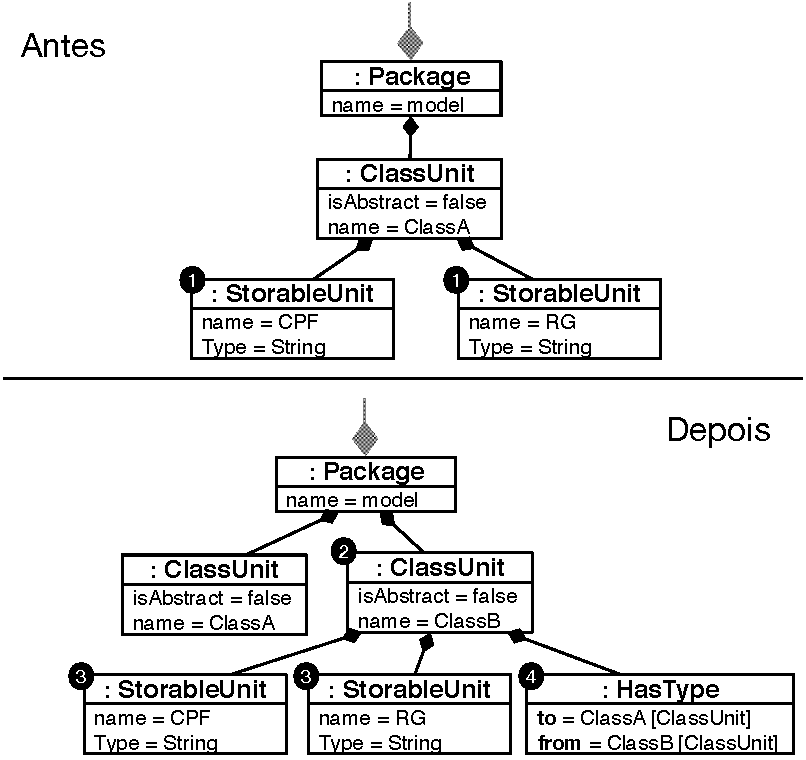
\includegraphics[scale=0.6]{images/antes_e_depois_refatoracao_extract_ClassUnit.pdf}
	\fautor
	\label{fig:antes_e_depois_extract_ClassUnit}
\end{minipage}\hfill
			\item Algoritmo: 
			    \begin{itemize}
			        \item createNewClassUnit(\{novoNome\});
			        \item adiciona essa nova instância dentro de um \texttt{Package};
			        \item para cada \{\texttt{StorableUnit}Selecionado\} - move(\{newClassUnit\}, \{\texttt{StorableUnit}Selecionado\})
			        \item para cada \{\texttt{MethodUnit}Selecionado\} - move(\{newClassUnit\}, \{\texttt{MethodUnit}Selecionado\});
			        \item createNewHasType(\{newClassUnit\}, \{\texttt{ClassUnit}Selecionada\}).
			    \end{itemize} 
	    \end{enumerate}
		\item Especificação Formal:
		\begin{enumerate}
			\item Pré-condição: 
			\begin{codigo}[caption={[OCL representando a pré-condição da refatoração \textit{Extract ClassUnit}.] Pré-condição da refatoração \textit{Extract ClassUnit}.},escapeinside={(*@}{@*)}, basicstyle=\footnotesize, label={codigo:pre_extract_ClassUnit}, language=OCL]{Name}
context ClassUnit::ExtractClassUnit(newName: String, storableUnitSelected:(StorableUnit), methodUnitSelected: (MethodUnit))
pre : newName.isValidName() and not self.refImmediateComposite().codeElement(*@$\rightarrow$@*)exist (c: ClassUnit | c.name = newName) 
and not storableUnitSelected(*@$\rightarrow$@*)forAll (s: StorableUnit | self.codeElement(*@$\rightarrow$@*)forAll (m: MethodUnit | not (m.codeRelation(*@$\rightarrow$@*)exists(re: Reads | re.to = s)) and not (m.codeRelation(*@$\rightarrow$@*)exists (wr:Writes | wr.to = s)) and not (m.codeRelation(*@$\rightarrow$@*)exists (add: Addresses | add.to = s)) 
and not methodUnitSelected(*@$\rightarrow$@*)forAll (m: MethodUnit | self.codeElement(*@$\rightarrow$@*)forAll (m: MethodUnit | not (m.codeRelation(*@$\rightarrow$@*)exists (call: Calls| call.to = m)))))
\end{codigo}
%É importante observar que deve-se especificar a \texttt{ClassUnit} que será renomeada, bem como definir o novo nome dessa \texttt{ClassUnit} antes de executar a pré-condição, como apresentado no Código-fonte~\ref{codigo:pre_renameClassUnit}. 
Na linha 1 do Código-fonte~\ref{codigo:pre_extract_ClassUnit} é declarado a assinatura da pré-condição da refatoração \textit{Extract ClassUnit}, note que essa pré-condição possui três parâmetros: o nome da nova instância da metaclasse \texttt{ClassUnit}, um conjunto de \{\texttt{StorableUnit}Selecionado\} e um conjunto de \{\texttt{MethodUnit}Selecionado\}. Na linha 2 é verificado se o parâmetro \{newName\} é válido para ser utilizado como nome de classe. Ainda na linha 2 a instância de da metaclasse \texttt{Package} é obtida por meio da função \texttt{refImmediateComposite()} para verificar dentro do escopo deste pacote se não existe nenhuma classe com o mesmo nome. Na linha 3 para cada \{\texttt{StorableUnit}Selecionado\} é verificado se são utilizados dentro de uma instância de \texttt{MethodUnit}, ou seja, verifica-se se o \{\texttt{StorableUnit}Selecionado\} é escrito e utilizado nos métodos. Similarmente, na linha 4 é verificado para cada \{\texttt{MethodUnit}Selecionado\} se o mesmo é chamado em algum lugar. Caso a pré-condição definida seja válida a refatoração \textit{Extract ClassUnit} é executada.
			\item Algoritmo: 
	\begin{codigo}[caption={[ATL representando a refatoração \textit{Extract ClassUnit}.] ATL da refatoração \textit{Extract ClassUnit}.},escapeinside={(*@}{@*)}, basicstyle=\footnotesize, label={codigo:extract_classUnit_ATL}, language=ATL]{Name}
module createAnClassThenMoveAnAttribute;
create OUT : MM refining IN : MM;
rule extractClassUnit {
	from
		source : MM!Package (source.name = (*@\aspas{\{\texttt{ClassUnit}Selecionada.refImmediateComposite()\}}@*))
	to 
		target: MM!Package (
			codeElement(*@$\leftarrow$@*)source.codeElement(*@$\rightarrow$@*)including(newClassUnit)
		),
		newClassUnit: MM!ClassUnit (
			name(*@$\leftarrow$@*)(*@\aspas{\{newName\}}@*),
			codeElement(*@$\leftarrow$@*)thisModule.getMethodUnits(thisModule.getClassUnit((*@\aspas{\{\texttt{ClassUnit}Selecionada\}}@*)), (*@\aspas{\{\texttt{MethodUnit}Selecionados\}}@*)),
			codeElement(*@$\leftarrow$@*)thisModule.getStorableUnits(thisModule.getClassUnit((*@\aspas{\{\texttt{ClassUnit}Selecionada\}}@*)), (*@\aspas{\{\texttt{StorableUnit}Selecionados\}}@*)))
rule createLinkExtractClassUnit {
	from
		source : MM!ClassUnit (source.name = (*@\aspas{\{\texttt{ClassUnit}Selecionada\}}@*))
	to 
		target: MM!ClassUnit (
			codeRelation(*@$\leftarrow$@*)source.codeRelation(*@$\rightarrow$@*)including(hasType)
		),
		hasType: MM!HasType (
			to(*@$\leftarrow$@*)(*@\aspas{\{\texttt{ClassUnit}Selecionada\}}@*),
			from(*@$\leftarrow$@*)(*@\aspas{\{new\texttt{ClassUnit}\}}@*)
		)
}}
helper def : getClassUnit (className : String) : MM!ClassUnit = MM!ClassUnit.allInstances()->any(e | e.name = className);
helper def : getStorableUnit (classUnitToGetTheStorableUnit: MM!ClassUnit, nameOfAtt: String) : MM!StorableUnit = classUnitToGetTheStorableUnit.codeElement(*@$\rightarrow$@*)any(e | e.name = nameOfAtt);		
helper def : getMethodUnits (classUnitToGet: MM!ClassUnit, nameMethod: String) : MM!MethodUnit = classUnitToGet.codeElement(*@$\rightarrow$@*)any(e | e.name.equalsIgnoreCase(nameMethod));
\end{codigo}
Na linha 1 do Código-fonte~\ref{codigo:extract_classUnit_ATL} o nome da refatoração é definido. Em seguida, na linha 2 é apresentado o cabeçalho da refatoração. Nas linhas 3 até 13 a primeira regra dessa refatoração é definida. Na linha 5 uma condição de guarda é definida para identificar a instância da metaclasse \texttt{Package} que a nova instância da metaclasse \texttt{ClassUnit} será adicionada. Em seguida, as linhas 7, 8 e 9 representam que uma nova instância de \texttt{StorableUnit} será criado dentro da instância do \texttt{Package} identificado. Nas linhas 10 e 11 uma nova instância da metaclasse \texttt{ClassUnit} é efetivamente criada. Posteriormente, nas linhas 12 e 13 os \{\texttt{StorableUnit}Selecionados\} e os \{\texttt{MethodUnit}Selecionados\} são movidos para a \texttt{ClassUnit} recém instanciada. Após mover os \{\texttt{StorableUnit}Selecionados\} e os \{\texttt{MethodUnits}Selecionados\} para a \texttt{ClassUnit} o próximo passo é criar uma associação entre as duas instâncias de \texttt{ClassUnit}. Esse passo é representado na regra descrita nas linhas 14 até 25. Na linha 17 a {\texttt{ClassUnit}Selecionada\} é identificada, depois as linhas 18, 19 e 20 sinalizam que uma instância da metaclasse \texttt{HasType} será criada. Finalmente, nas linhas 21 até 23 a instância da metaclasse \texttt{HasType} é criada. Mas especificadamente, nas linhas 22 e 23 seus relacionamentos \texttt{to} e \texttt{from} são definidos, os quais representam a associação entre a classe que continha os \{\texttt{StorableUnit}Selecionados\} e os \{\texttt{MethodUnits}Selecionados\} e a nova instância da metaclasse \texttt{ClassUnit}, respectivamente. Linhas 26, 27 e 28 os \textit{helpers} que são utilizadas nessa refatoração são definidos.   
			\item Pós-condição:
			 \begin{codigo}[caption={[OCL representando a pós-condição da refatoração \textit{Extract ClassUnit}.] Pós-condição da refatoração \textit{Extract ClassUnit}.},escapeinside={(*@}{@*)}, basicstyle=\footnotesize, label={codigo:pos_condicao_extract_ClassUnit}, language=OCL]{Name}
context ClassUnit::ExtractClassUnit(storableUnitSelected: (StorableUnit), methodUnitSelected: (MethodUnit), newClass: ClassUnit)
post : self.codeElement(*@$\rightarrow$@*)exists (s: StorableUnit | not (storableUnitSelected(*@$\rightarrow$@*)forAll (sUS: StorableUnit | sUS.name = s.name))) and self.codeElement(*@$\rightarrow$@*)exists (m: MethodUnit | not (methodUnitSelected(*@$\rightarrow$@*)forAll (mUS: MethodUnit | mUS.name = m.name))) 
and newClass.codeElement(*@$\rightarrow$@*)exist (s: StorableUnit | (storableUnitSelected(*@$\rightarrow$@*)forAll (sUS: StorableUnit | sUS.name = s.name))) and newClass.codeElement(*@$\rightarrow$@*)exists (m: MethodUnit | not (methodUnitSelected(*@$\rightarrow$@*)forAll (mUS: MethodUnit | mUS.name = m.name)))        \end{codigo}
Na linha 1 do Código-fonte~\ref{codigo:pos_condicao_extract_ClassUnit} é declarado o nome da pós-condição. Na linha 2 é verificado se todos os \{\texttt{StorableUnit}Selecionados\} e \{\texttt{MethodUnits}Selecionados\} não estão definidos na \{\texttt{ClassUnit}Selecionada\}. Posteriormente, na linha 3, é verificado se todos os \{\texttt{StorableUnit}Selecionados\} e \{\texttt{MethodUnits}Selecionados\} foram efetivamentes movidos para a nova instância da metaclasse \texttt{ClassUnit}. Caso afirmativo a refatoração foi realizada com sucesso.
		\end{enumerate}
\end{enumerate}
	
	
\section{Considerações Finais}\label{sec:consideracoes_finais_capitulo_reforacao}

Neste capítulo foram apresentadas cinco diretrizes para auxiliar o engenheiro de modernização a criar refatorações para o metamodelo KDM. Com o intuito de exemplificar essas cinco diretrizes foram escolhidas algumas refatorações propostas por~\citeonline{Fowler1999} para serem criadas para o metamodelo KDM. Embora ~\citeonline{Fowler1999} tenha definido um catálogo de refatoração para ser utilizado em código-fonte, mais de 60\% das refatorações (44 de 72) são ilustradas e explicadas utilizando modelos, mais especificadamente diagramas de classes da UML. Esta observação fez com que tais refatorações fossem criadas para o metamodelo KDM. 

Antes de criar qualquer refatoração para o metamodelo KDM, a primeira diretrizes diz que é  necessário identificar as metaclasses do KDM que têm características similares aos conceitos do POO, bem como instruções comumente utilizadas em todas as linguagens de programação, tais como, ramificações, iterações, etc. Dessa forma, esse capítulo também apresentou um mapeamento entre os conceitos do POO e o metamodelo KDM. Acredita-se que engenheiros de modernização pouco familiarizado com o metamodelo KDM podem gastar menos tempo durante a criação de novas refatorações com a utilização deste mapeamento, assim, qualquer exemplo de refatoração pode ser facilmente adaptada para o metamodelo KDM seguindo esse mapeamento, bem como as diretrizes aqui apresentadas.

Após identificar todos os elementos estruturais e identificar o mapeamento entre POO e o metamodelo KDM, o próximo passo é escolher qual refatoração criar. No contexto desta Tese todas as refatorações podem ser agrupadas em nível de granularidade. As granularidades podem ser definidas em dois níveis de operações: (\textit{i}) operação atômica e (\textit{ii}) operações compostas. As granularidades definidas como operações atômicas podem ser especificas por meio de operações primitivas (\texttt{addd}, \texttt{delete} e \texttt{change}). As refatorações de granularidade compostas são uma combinação de operações atômicas (ver Tabela~\ref{tab:refatoringsCatalogo}). Em seguida na próxima diretriz o engenheiro de modernização deve implementar a refatoração por meio da linguagem de transformação ATL. Então o engenheiro de modernização deve implementar as restrições (pré- e pós-condições) da refatoração.

Após criar uma determinada refatoração, bem como suas pré- e pós-condições para o metamodelo KDM, o engenheiro de modernização deve especificar e documentar a refatoração. As refatoração criadas para o metamodelo KDM consistem de duas principais especificações - uma especificação informal e uma especificação formal. Na especificação informal a ideologia básica é permitir que o engenheiro de modernização expresse o propósito da refatoração por meio de linguagem natural. A segunda especificação é responsável por representar as pré- e pós-condições, bem como a transformação/refatoração propriamente dita em linguagens executáveis - OCL e ATL foram utilizadas, respectivamente. Ambas especificações são úteis para o engenheiro de modernização -a especificação informal é utilizada para facilitar a compreensão e o propósito da refatoração,enquanto que a especificação formal facilita a implementação da refatoração. Além disso, a especificação formal é de extrema importância para facilitar a automação das refatorações. %É importante destacar que neste capítulo apenas as refatorações \textit{Rename ClassUnit}, \textit{Pull Up StorableUnit}, \textit{Push Down StorableUnit} e \textit{Extract ClassUnit} são apresentadas e detalhadas.

Seguindo as diretrizes apresentada neste capítulo o engenheiro de modernização pode criar refatorações para o metamodelo KDM. No entanto, as especificações formais e informais resultantes não são suficientes para promover o reúso de refatorações no contexto do metamodelo KDM. Dessa forma, no Capítulo~\ref{chapter:Toward_a_Refactoring_Metamodel_for_KDM} é apresentado um metamodelo para auxiliar o engenheiro de modernização a promover o reúso de refatorações no contexto do metamodelo KDM. Com a utilização desse metamodelo, informações (metadados) sobre refatorações podem ser reutilizadas de forma independente de linguagem e plataforma. No Capítulo~\ref{chapter:Abordagem_de_sincronizacao} uma abordagem para manter instâncias do metamodelo KDM sincronizada e consiste após a aplicação de refatoração é apresentada. No Capítulo~\ref{chapter:ferramenta_kdm_re} é apresentado uma ferramenta que foi desenvolvida dentro do ambiente Eclipse para apoiar o uso do catálogo de refatoração adaptado para o metamodelo KDM, dessa forma, essa ferramenta permite que modernizadores apliquem refatorações diretamente no metamodelo KDM. 


\chapter{SRM: Um Metamodelo para Promover o Reúso das Refatorações para o KDM}
\label{chapter:Toward_a_Refactoring_Metamodel_for_KDM}
\section{Considerações Iniciais}\label{sec:consideracoes_iniciais}
Geralmente refatorações são aplicadas para melhorar a qualidade do software (por exemplo, a extensibilidade, a modularidade, a capacidade de reutilização, a complexidade, manutenção, etc). 
A maioria das pesquisas apontam que usualmente refatorações são aplicadas em nível de código-fonte~\cite{Fowler1999, Demeyer1, Demeyer2, Opdy92b}. Tais pesquisas não estão preocupadas em como promover o reuso, compartilhamento de refatorações e também não estão interessadas em criar refatorações para outros tipos de artefatos, tais como os artefatos providos pela ADM, por exemplo, o metamodelo KDM. 
%
Como já destacado, na literatura é possível identificar um conjunto de refatorações já validadas e que são usualmente aplicadas em código-fonte, por exemplo, \textit{Extract Class}, \textit{Move Method}, \textit{Move Attribute}, etc. Essas são apenas alguns exemplos de refatorações úteis que não são facilmente reutilizadas na prática durante a condução de modernização de um determinado sistema. Essa limitação pode ser atribuída devido a ausência de um meio padronizado de disponibilizar refatorações. 
Uma abordagem promissora é lidar com a refatoração de forma independente da linguagem – aumentando assim as possibilidades de reutilização de refatorações.

Como ressaltado no Capítulo~\ref{chapter:adm_kdm} a ADM fornece um conjunto de metamodelos para auxiliar o engenheiro de software a conduzir MDRE. 
Porém, até esse momento a ADM não provê instruções ou até mesmo um metamodelo para auxiliar o engenheiro a promover o reuso de refatorações juntamente com os seus metamodelos padronizados (por exemplo, KDM) durante o processo de modernização. 
Essa limitação faz com que o engenheiro de modernização crie suas próprias soluções/refatorações, resultando em um possível atraso no processo de modernização. 
No Capítulo~\ref{chapter:catalogo_refactoring_KDM} algumas refatorações bem conhecidas e propostas por~\citeonline{Fowler1999} são adaptadas para serem aplicadas em instâncias do metamodelo KDM. Contudo, em seu estado atual as refatorações adaptadas não podem serem facilmente reutilizadas e compartilhadas entre os modernizadores. 
Com o intuito de suprir tal limitação neste capítulo é apresentado um metamodelo para auxiliar o engenheiro de modernização a promover o reuso de refatorações no contexto do metamodelo KDM. Com a utilização desse metamodelo, informações (metadados) sobre refatorações podem ser reutilizadas de forma independente de linguagem e plataforma. 

O metamodelo aqui proposto tem as seguintes características: (\textit{i}) permite a interoperabilidade de refatorações para um amplo domínio e (\textit{ii}) auxilia o engenheiro de modernização a definir refatorações representativas em forma de metadados. Nota-se que o metamodelo aqui proposto segue a mesma proposta de outros metamodelos definidos na ADM e está totalmente integrado com o metamodelo KDM. Em outras palavras, uma instância do metamodelo de refatoração contêm metadados que representam uma refatoração escrita para ser executada em uma instância do metamodelo KDM. A escolha do metamodelo KDM se deu pois o mesmo é um metamodelo padronizado pela OMG, além de ser um metamodelo PIM, o que significa que quaisquer refatorações aplicadas em uma instância do KDM, podem ser consideradas independentes de linguagem e de plataforma e então ser transformado para em um PSM (ver Capítulo~\ref{chapter:fundamentacao_teorica} e Capítulo\ref{chapter:adm_kdm}). Utilizar refatorações como um metamodelo (de forma independente de linguagem) pode abrir opções para promover o reuso de refatorações. Por exemplo, dado uma instância do metamodelo de refatoração, o engenheiro de modernização poderia utilizar os metadados contidos nessa instância e aplicar a refatoração em qualquer sistema representado pelo KDM. Além disso, o engenheiro de modernização poderia instanciar o metamodelo de refatoração, criar um catálogo de refatorações e disponibilizar para que outros possam reutilizar tais refatorações. Tornando assim possível compartilhar e reutilizar refatorações no contexto da ADM.

%Com o intuito de apresentar o metamodelo de uma maneira mais prática, neste capítulo a construção do mesmo é realizado com o uso do EMF~\cite{EMF}. Porém, ressalta-se que o metamodelo pode ser criado com o uso de outras tecnologias.

As demais seções deste capítulo estão organizadas da seguinte forma: na Seção.... é apresentada a motivação para a criação do metamodelo de refatoração; na Seção ... o metamodelo é apresentado..., na Seção .. são feitas as considerações finais a respeito do metamodelo de refatoração proposto neste capítulo.\change{terminar aqui. Deve colocar todas as seções bem escritas.}

\section{Motivação para a criação de um metamodelo de refatoração} % (fold)
\label{sec:motiva_o_para_a_cria_o_de_um_meta_modelo_de_refatora_o}

Durante o mapeamento sistemático conduzido (ver Capítulo~\ref{chapter:mapeamento_sistematico})~\cite{durelli_systematic_mapping} pôde-se observar na literatura a carência de estudos que definem soluções para especificar e promover o reuso de refatorações no contexto da ADM e do metamodelo KDM. Sem a adequada representação de refatorações para o KDM, a especificação e realização de uma refatoração pode se tornar uma atividade propensa a erros e difícil de reutilizar.

Neste contexto, suponha o seguinte cenário, um engenheiro de modernização define uma determinada refatoração e a compartilha por meio de um repositório. Dessa forma, outros engenheiros podem então navegador nesse repositório e identificar, não apenas essa, mas um conjunto de refatorações. O engenheiro então escolhe uma determinada refatoração no repositório, faz o \textit{download} e a reutiliza em seu sistema representado em nível de uma instância do metamodelo KDM. 

Uma das soluções para a concretização desse cenário seria a criação de um metamodelo para persistir metadados referentes à refatorações. Esse metamodelo deve possuir metaclasses e meta-relacionamentos que permitam representar e especificar metadados de refatorações, por exemplo, o nome da refatoração, sua motivação, os passos para sua realização, e até mesmo o mecanismo e sua pré- e pós-condições. Como ressaltado anteriormente, devido a carência de um metamodelo que possui tais características, esse capítulo têm como principal objetivo definir um metamodelo que permita a representação de metadados relacionadas com refatorações, porém, ainda respeite e siga as diretrizes dos metamodelos definidos na abordagem ADM, por exemplo, o metamodelo aqui definido precisa ser independente de linguagem e plataforma.


Essa ultima características é de suma importância. Assim, o metamodelo aqui apresentado utiliza as metaclasses do metamodelo KDM. Uma instância do metamodelo de refatoração, deve possuir instâncias de metaclasses específicas para definir metadados sobre refatorações (autor, nome, motivação, descrição, etc) e também instâncias de metaclasses do KDM que representam os elementos estruturais (\texttt{ClassUnit}, \texttt{StorableUnit}, \texttt{MethodUnit}, etc) onde a refatoração/transformação será aplicada. Dessa forma, o metamodelo de refatoração faz com que a operação/mecanismo de uma refatoração torne-se independente de plataforma e linguagem de programação. Assim, o metamodelo pode ser facilmente utilizado e aplicado em ferramentas existentes que utilizam como base o KDM aumentando a interoperabilidade de futuras ferramentas que utilizem esse metamodelo de refatoração. Levando em consideração as motivações destacadas, na Seção~\ref{sec:meta_modelo_de_refatora_es_estruturadas_srm_do_ingl_s_structured refactoring meta-model_} é apresentado o metamodelo de refatorações estruturadas (do inglês - Structured Refactoring Metamodel – SRM).  


%Além disso, uma característica de suma importância é que esse metamodelo de refatoração seja baseado nas metaclasses do KDM. Em outras palavras, uma instancia desse metamodelo, deve conter referencias a metaclasses do KDM, tornando assim, a operação/mecanismo de um refatoração independente de plataforma e linguagem. 

\section{Metamodelo de Refatorações Estruturadas} % (fold)
\label{sec:meta_modelo_de_refatora_es_estruturadas_srm_do_ingl_s_structured refactoring meta-model_}

Como pôde ser observado na seção anterior, são várias as motivações para definir um metamodelo para especificar refatorações. Neste sentido, nesta seção é apresentado um metamodelo denominado Metamodelo de Refatorações Estruturadas (do inglês - \sigla{SRM}{Structured Refactoring Metamodel}).

Refatorações são ubíquas durante a manutenção, produção e análise de software. Inúmeras comunidades têm surgido na literatura para criar e definir vários tipos de refatorações, incluindo refatorações de baixa granularidade~\cite{Fowler1999, Demeyer1, Demeyer2}, refatorações arquiteturais, refatorações para o paradigma orientado a aspecto, etc. Neste contexto, existe a necessidade de definir uma forma de promover o compartilhamento dessas refatorações. Assim, nessa seção é apresentado um metamodelo para auxiliar tais comunidades. Esse metamodelo representa uma fundamentação para o compartilhamento de informações (metadados) relacionadas à refatorações, assim, detalhes com informações precisas sobre refatorações podem ser armazenadas e/ou compartilhadas para que outros engenheiros possam reutilizar em seus projetos que utilizem o metamodelo KDM.

Por exemplo, uma comunidade que cria refatorações de baixa granularidade usualmente esta preocupada em definir e especificar refatorações desse tipo. Por outro lado, uma comunidade que especifica refatorações arquiteturais esta interessada apenas em refatoração arquiteturais. Porém, nota-se que ambas comunidades têm em comum a necessidade de especificar como organizar e definir as refatorações. Além disso, tais comunidades devem se preocupar em definir a motivação para a condução da refatoração, especificar o mecanismo da refatoração e descrever tais refatorações de maneira formal e adequada para a sua comunidade. Embora o contexto dessas comunidades seja diferentes ambas necessitam de uma forma padronizada para definir e especificar as refatorações. 


O SRM define um padrão comum para a especificação e descrição de refatorações. Além disso, esse metamodelo têm como princípio ser independente de linguagem de programação com o objetivo de fornecer uma plataforma comum pelo qual arquiteto, pesquisador e modernizador possam expressar refatorações sem se preocuparem com a plataforma ou linguagem de programação. O SRM possui três principais objetivos: (\textit{i}) prover uma forma de compartilhar informações sobre refatorações; (\textit{ii}) promover o reuso de refatorações de forma independente de plataforma e linguagem; e (\textit{iii}) ser uma proposta inicial ao \textit{Call for Proposals} do ADM Refatoring da OMG. O primeiro objetivo é apoiada por um conjunto de metaclasses que definem meta-atributos específicos para representar informações (metadados) de uma refatoração, auxiliando assim o compartilhamento das refatorações de forma intuitiva para os modernizadores. Similarmente, o segundo objetivo também é alcançado por metaclasses que possuem meta-atributos que representam os mecanismos das refatorações, bem como suas pré- e pós-condições. O terceiro objetivo é apoiado por todo o metamodelo SRM.
 
Na Figura~\ref{fig:refactoring_metamodel} o SRM é esquematicamente apresentado. O centro da figura representa a abordagem ADM. Pode-se entender que o SRM está inserido no contexto da ADM da mesma forma que seus outros metamodelos. A esfera externa é dividida em quatro facetas, cada uma contêm o nome de um metamodelo – por sua vez, cada faceta é acoplada por um retângulo contendo o nome de um metamodelo e um conjunto de metaclasses. Como pôde ser observado nessa figura o SRM está inserido no contexto da ADM para preencher a definição de um metamodelo de refatorações. 

Um dos objetivos do SRM é seguir as padronizações propostas pela ADM. Porém, deve-se ressaltar que o SRM é utilizado para especificar a representação de refatorações sem se preocupar com a representação das partes estruturais de uma refatoração, ou seja, os elementos que serão refatorados (classes, métodos, atributos, etc.). Assim, o SRM assume que tais elementos (classes, métodos, atributos, etc.) devem ser representados utilizando outro metamodelo proposto pela ADM, neste contexto o KDM. Como visualizado na Figura~\ref{fig:refactoring_metamodel}, o SRM interage com o metamodelo KDM para utilizar instâncias de metaclasses do KDM para representar os elementos que serão refatorados. Consistente com outros metamodelos definidos pela OMG, o SRM é definido utilizando a padronização de modelagem MOF e a \textit{framework} EMF. Um dos benefícios de utilizar MOF é que o mesmo permite que o metamodelo seja serializado e deserializado sem perder nenhum tipo de informação, ou seja, metamodelos instanciados são representados utilizando uma representação textual padronizada, XMI. Além disso, o SRM é compatível com repositórios MOF para armazenamento e recuperação de várias ferramentas, aumentando assim a interoperabilidade de futuras ferramentas que utilizem esse metamodelo.

\begin{figure}[h]
	\centering
	% Requires \usepackage{graphicx}
	\caption{Integração do SRM com outros metamodelos da ADM.}
	\label{fig:refactoring_metamodel}
	\includegraphics[scale=0.65]{images/SRM2Formatted}
	\fautor
\end{figure}


A Figura~\ref{fig:fases_para_a_construcao_e_uso_do_SRM} apresenta uma macro-visão da engenharia do metamodelo SRM utilizando a notação \sigla{SADT}{\textit{Structured Analysis and Design Technique}}~\cite{Marca_1987}. Como observado um conjunto de elementos foram utilizados como base para o desenvolvimento do SRM: elementos estruturais, linguagens de transformações, linguagens de restrições e catálogos de refatorações. A seguir, na Subseção~\ref{Engenharia_do_Meta_modelo_SRM} esses elementos são apresentados e comentados como foram utilizados para desenvolver o metamodelo SRM.

\begin{figure}[h]
	\centering
	% Requires \usepackage{graphicx}
	\caption{Fases para a construção e uso do SRM.}
	\label{fig:fases_para_a_construcao_e_uso_do_SRM}
	\includegraphics[scale=0.9]{images/SRM_Construcao2}
	\fautor
\end{figure}

\subsection{Engenharia do SRM}\label{Engenharia_do_Meta_modelo_SRM}

Refatorações, suas características e terminologia foram analisadas para que o SRM fosse desenvolvido. Antes de iniciar a criação do metamodelo SRM (ou de qualquer outro metamodelo) é necessário definir os elementos que deverão ser representados e as relações entre eles. Nesse sentido, cinco etapas que compõem a engenharia do SRM são mostradas na Figura~\ref{fig:etapas_da_fase_de_e_do_SRM}: (\textit{i}) Identificação dos Elementos Estruturais, (\textit{ii}) Identificação das Linguagens de Transformações, (\textit{iii}) Identificação das Linguagens de Restrições, (\textit{iv}) Identificação de vocabulário/termos/conceitos e (\textit{v}) Projeto e criação do metamodelo SRM. 

\begin{figure}[h]
	\centering
	% Requires \usepackage{graphicx}
	\caption{Etapas da fase de Engenharia do SRM.}
	\label{fig:etapas_da_fase_de_e_do_SRM}
	\includegraphics[scale=0.75]{images/todasAsFasesDaEngenhariaDOSRM6}
	\fautor
\end{figure}



\subsection{Identificação dos Elementos Estruturais}

Esta etapa possui como objetivo analisar e identificar possíveis elementos estruturais para serem utilizados durante a refatoração. No Capítulo~\ref{chapter:catalogo_refactoring_KDM} Seção~\ref{sec:mapeamento_POO_e_KDM}, a Tabela~\ref{tab:mapemanetoEntreOOPeKDM} apresenta uma relação existente entre os conceitos do POO, bem como algumas instruções de linguagens de programção e o metamodelo KDM. Para fazer com o que o metamodelo SRM seja independente de linguagem e plataforma foi utilizado os elementos (metaclasses) do KDM para representar os elementos estruturais. Como já salientado no Capítulo~\ref{chapter:catalogo_refactoring_KDM}, o metamodelo KDM contêm algumas metaclasses que podem ser diretamente mapeadas a elementos estruturais, tal como, classes (\texttt{ClassUnit}), interfaces (\texttt{InterfaceUnit}), atributos (\texttt{StorableUnit}), métodos (\texttt{MethodUnit}), etc. Essas metaclasses possuem o mesmo objetivo e características dentro do contexto do POO e linguagens de programação. %Entretanto, como o KDM tem como objetivo ser um modelo independente de plataforma, ou seja, tem como intuito representar de forma genérica todas as abstrações e paradigmas de programação, algumas construções de programação não possuem uma metaclasse particular. Por exemplo, iterações e ramificações em KDM são representadas utilizando a mesma metaclasse, \texttt{ActionElement}.

Elementos estruturais no contexto deste capítulo representam as instâncias das metaclasses que serão refatorados, por exemplo, \texttt{ClassUnit}, \texttt{MethodUnit}, \texttt{StorableUnit}, etc. Tais metaclasses foram consideradas boas candidatas para facilitar o reuso e troca de metadados no metamodelo SRM. Por exemplo, considere a refatoração \textit{RenameX}, onde \textit{X} pode ser qualquer elemento estrutural (\texttt{ClassUnit}, \texttt{MethodUnit}, \texttt{StorableUnit}, etc.). Os passos e mecanismo necessários para realizar essa refatoração são iguais ou possuem poucas diferenças não importa o tipo de elemento estrutural que será refatorado. Tendo como base esse exemplo, é possível identificar a necessidade de representar os metadados dos elementos estruturais que serão refatorados no SRM. Como o KDM (ver Capítulo~\ref{chapter:adm_kdm}) foi desenvolvido com o intuito de representar todo o sistema e seus artefatos – o mesmo é um bom candidato para representar os elementos estruturais de uma refatoração. Portanto, nesta etapa as metaclasses do metamodelo KDM foram consideradas boas candidatas para serem os elementos estruturais das refatorações. Dessa forma, como apresentado na Figura~\ref{fig:refactoring_metamodel} ambos metamodelos, SRM e KDM, são utilizados juntamente para a definir refatorações em nível de metadados.

\subsection{Identificação das Linguagens de Transformações}

Nesta etapa são identificadas e analisados os detalhas de um conjunto de linguagens de transformações com o intuito de identificar as informações necessários para promover o reuso do mecanismo das refatorações. 

Conceitualmente, refatorações são definidas por meio de um conjunto de passos que devem ser seguidos para realizar uma determina mudança~\cite{Fowler1999, Demeyer1}. Por outro lado, programaticamente as refatorações são definidos como \aspas{programas} parametrizados que executam um conjunto de transformações seguindo uma ordem lógica. Usualmente, no contexto de modelos, tais transformações são conhecidas como endógenas e são implementadas utilizando técnicas de reescrita de grafo, ou como também é conhecida transformação de grafo (ver Capítulo~\ref{chapter:fundamentacao_teorica} Seção~\ref{sec:transformacoes_de_modelos}). Dessa forma, pode-se caracterizar que técnica de reescrita de grafo é útil para auxiliar na elaboração de transformações de forma independente para \textit{n} metamodelos, ou seja, técnica de reescrita de grafo pode ser aplicada em qualquer metamodelo que implemente o padrão MOF, como por exemplo o metamodelo KDM. 

Comumente, transformações em modelos são definidas utilizando linguagens específicas de transformações de modelos. Diversas linguagens de transformação de modelos têm sido propostas atualmente~\cite{Biehl_2010, Allilaire_06}, entre elas pode-se citar ATL e QVT. Por exemplo, no Código-fonte~\ref{codigo:rename_classUnit_SRM} é apresentado um trecho da refatoração \texttt{Rename ClassUnit} escrito em ATL. Por meio da linguagem de programação ATL facilmente pode-se especificar qual metamodelo esta sendo utilizado na refatoração. Além disso, com o uso da ATL e QVT pode-se automatizar os mecanismos e todos os passos que uma determinada refatoração deve realizar. Por exemplo, no Código-fonte~\ref{codigo:rename_classUnit_SRM} uma determinada instância de \texttt{ClassUnit} que contêm o meta-atributo \texttt{name} igual à \aspas{Fusca} será refatorada para \aspas{Ferrari}. Dessa forma, com o propósito de automatizar os mecanismo e todos os passos de uma refatoração no contexto do metamodelo SRM, tanto ATL e QVT foram consideradas boas candidatas para especificar programaticamente os metadados sobre o mecanismo das refatorações. %ATL e QVT foram escolhidas como linguagens de transformação nesta capítulo considerando vários aspectos. Tais linguagens estão integradas na plataforma Eclipse, o que fornece uma série de recursos padrões para o desenvolvimento (\textit{syntax highlighting} e \textit{debugger}). Ambas linguagens são parte do projeto \textit{Model-To-Model} e possuem um grupo de discussão ativo, constantemente atualizado, vários exemplos e diversos estudos de casos aplicados até mesmo na indústria utilizam tais linguagens.


\begin{codigo}[caption={[Refatoração \textit{Rename ClassUnit}.] Refatoração \textit{Rename ClassUnit}.},escapeinside={(*@}{@*)}, basicstyle=\footnotesize, label={codigo:rename_classUnit_SRM}, language=ATL]{Name}
module renameClassUnit;
create OUT : MM refining IN : MM;
rule renameClassUnit {
	from
		source : MM!ClassUnit (source.name = (*@\aspas{Fusca}@*))
	to 
		target : MM!ClassUnit (
			name (*@$\leftarrow$@*) (*@\aspas{Ferrari}@*)
		)
}
\end{codigo}



%Linguagem de transformação representam as operações/mecanismos de um refatoração. Tais operações/mecanismos são responsáveis por realizar a refatoração propriamente dita no metamodelo. Usualmente  tais transformações são escritas em linguagens imperativas como \textit{Query}/\textit{View}/-\textit{Transformation} (QVT) ou ATL \textit{Transformation Language}.

\subsection{Identificação das Linguagens de Restrições}
Nesta etapa as formas de especificar as restrições são identificadas para definir as pré- e pós-condições de uma determinada refatoração. É importante que o metamodelo SRM permita definir tais restrições e não apenas o mecanismo da refatoração, assim, engenheiros podem utilizar uma determinada instância do metamodelo SRM e verificar quais são as restrições que eles devem respeitar para executar a refatoração de forma correta. Tais restrições no contexto de refatorações são conhecidas como pré- e pós-condições\cite{OPDYKE_1992, Roberts_1999}.

Usualmente antes e após executar uma determinada refatoração algumas restrições precisam ser satisfeitas. Tais restrições usualmente são úteis para verificar se os parâmetros necessários para executar a refatoração foram completamente e corretamente informados, bem como verificar se a refatoração foi aplicada de forma totalmente correta. Além disso, restrições são úteis para garantir que a sintaxe e semântica do modelo sejam preservadas após a aplicação das refatorações, assegurando assim uma possível preservação de comportamento. No contexto de modelos, tais restrições podem ser especificadas utilizando linguagens como a padronização definida pelo OMG denominada OCL e XQuery. Por meio dessas linguagens, é possível verificar, por exemplo, se todos os parâmetros obrigatórios para executar a refatoração foram especificados pelo engenheiro de modernização. Assegurar que a refatoração será aplicada de forma correta é de suma importância para preservar a sintaxe e semântica da instância do metamodelo, como por exemplo, preservar comportamentos, sincronização, etc. 

Com o propósito de automatizar as pré- e pós-condições de uma refatoração no contexto do metamodelo SRM, tanto OCL e XQuery foram considerados boas candidatas para especificar programaticamente as restrições que devem ser satisfeitas e respeitadas para a execução da refatoração.

%Condições prévias de refatoração são propriedades do programa original que deve segurar por um refactoring ser de preservação comportamento.


%Linguagem de restrição no contexto desse capítulo representa pré- e pós-condição de uma refatoração. Usualmente no contexto de modelos, restrições podem ser escritas utilizando a \textit{Object Constraint Language} (OCL).

\subsection{Identificação de vocabulário/termos/conceitos}

Nesta etapa é realizada a identificação de vocabulário, termos e conceitos comuns que são utilizadas dentro da comunidade de refatoração. Durante a criação de metamodelos é de suma importância entender o domínio que o metamodelo representa. metamodelos definem abstrações (termos), notações e relacionamentos para representar um determinado domínio. Assim, nesta etapa tanto os vocabulários, termos e conceitos definidos por~\citeonline{OPDYKE_1992} e \citeonline{Fowler1999} foram analisados para a identificação de abstrações para facilitar a criação do metamodelo SRM. Durante a análise pode-se observar e identificar alguns termos comumente utilizados durante a definição de uma refatoração. Por exemplo, todas as refatorações descritas e definidas por~\citeonline{OPDYKE_1992} e \citeonline{Fowler1999} seguem os seguintes termos: 

\begin{itemize}
\item Refatoração: o nome da refatoração
\item Autor: autor da refatoração;
\item Catálogo: o catalogo no qual a refatoração pertence;
\item Biblioteca de refatoração: onde um conjunto de catálogos podem ser incluídos;
\item Descrição: informando uma típica situação onde a refatoração deveria ser aplicada;
\item Motivação: informando a motivação para a realização da refatoração;
\item Operação: descrevendo os passos que devem ser realizados para executar a refatoração;
\item Parâmetros: informações necessários para executar a operação da refatoração;
\item Restrições: Asserções utilizadas para garantir a semântica e sintaxe após a aplicação da refatoração;
\begin{itemize}
\item Pré-condição: asserção que deve ser verdadeira antes de executar a operação da refatoração;
\item Pós-condição: asserção que deve ser verdadeira após executar a operação da refatoração;
\end{itemize}
\end{itemize}

Utilizando os termos identificados nos trabalhos de~\citeonline{OPDYKE_1992} e ~\citeonline{Fowler1999} foi possível criar o metamodelo SRM. 

\subsection{Projeto e criação do Metamodelo SRM}

Nesta etapa o SRM é especificado a partir das informações extraídas nas etapas anteriores. Utilizando as informações extraídas foi possível identificar terminologias, bem como palavras-chaves que geralmente estão relacionadas com refatoração. Utilizando tais terminologias e palavras-chaves foi possível realizar a especificação do SRM. O SRM pode ser definido como uma quadrupla, como observado na Definição~\ref{def:SRM}: 


\begin{definicao}\label{def:SRM}
    \textit{O SRM é uma quadrupla $SRM = (SRM_{mC}, SRM_{mA}, SRM_{e}, SRM_{mR})$ onde $SRM_{mC} $ representa um conjunto de metaclasses, $SRM_{mA}$ representa um conjunto de meta-atributos, $SRM_{e}$ representa um conjunto de enumerações e $SRM_{mR}$ representa associações.}
\end{definicao}

Formalmente pode-se definir o metamodelo como:

\begin{itemize}
	\item Todas as metaclasses \textit{mC} $\in SRM_{mC}$ tem um nome que representa o seu significado;
	\item Todos os meta-atributos \textit{mA} $\in SRM_{mA}$ contêm um nome, um tipo e uma cardinalidade. Além disso, cada mA está associado a uma metaclasse;
	\item Todas as enumerações \textit{e} $\in SRM_{mA}$ contêm um nome e um valor;
	\item Todas as meta-associações \textit{mR} $\in SRM_{mR}$ é um conjunto R = $E_{1}$, $E_{2}$  , onde  $E_{1}$ e $E_{2}$ são associações de R. Posteriormente, cada R, contêm um nome. Ambos $E_{1}$  e $E_{1}$ possuem uma cardinalidade e são associados a uma metaclasse de $SRM_{mC}$.
\end{itemize}

Na Figura~\ref{fig:meta_modelo_SRM} é apresentado o metamodelo SRM. O SRM contêm 12 metaclasses e três enumerações. Um descrição detalhada de cada elementos desse metamodelo é apresentado a seguir:

\begin{figure}[h]
	\centering
	% Requires \usepackage{graphicx}
		\caption{Metamodelo SRM.}
	\includegraphics[scale=0.65]{images/refactoring_metamodel}
	\label{fig:meta_modelo_SRM}
	\fautor
\end{figure}

\begin{itemize}
\item \texttt{RefactoringModel} representa a metaclasse raiz do metamodelo.

\begin{itemize}
	\item \textbf{Associações}
		\begin{itemize}
			\item \texttt{author:Author[0..1]}: representa o autor de uma refatoração; 
			\item \texttt{libraries:RefactoringLibrary[0..*]}: representa um conjunto de biblioteca de refatorações que uma instância da metaclasse \texttt{RefactoringModel} possui..
		\end{itemize}
\end{itemize}

\item \texttt{Author} representa o autor de uma refatoração. Essa metaclasse contêm dois meta-atributos.

\begin{itemize}
	\item \textbf{Meta-atributos}
		\begin{itemize}
			\item \texttt{name}: utilizado para definir o nome do autor;
			\item \texttt{lastName}: utilizado para definir o sobrenome do autor.
		\end{itemize}	
\end{itemize} 

\item \texttt{RefactoringLibrary} utilizado para descrever uma biblioteca de refatorações.

\begin{itemize}
	\item \textbf{Attributes}
		\begin{itemize}
			\item \texttt{name}: utilizado para descrever o nome da biblioteca de refatoração;
			\item \texttt{shortDescription}: representa uma breve descrição sobre a biblioteca de refatoração;
			\item \texttt{description}: representa uma completa descrição sobre a biblioteca de refatoração.
		\end{itemize}	
\end{itemize} 

\begin{itemize}
	\item \textbf{Associação}
		\begin{itemize}
			\item \texttt{catalogs:Catalog[0..*]}: um conjunto de catálogos que contem refatorações.
		\end{itemize}	
\end{itemize} 

\item \texttt{Catalog} metaclasse utilizada para representar um catalogo de refatorações.

\begin{itemize}
	\item \textbf{Meta-atributos}
		\begin{itemize}
			\item \texttt{name}: representa o nome do catálogo. 
		\end{itemize}	
\end{itemize} 

\begin{itemize}
	\item \textbf{Associações}
		\begin{itemize}
			\item \texttt{author:Author[0..1]}: representa o autor do catalogo;
			\item \texttt{refactorings:Refactoring[0..*]}: conjunto de todas as refatorações que um catalogo contêm.
		\end{itemize}	
\end{itemize} 

\item \texttt{Refactoring} representa uma das principais metaclasses do SRM.

\begin{itemize}
	\item \textbf{Meta-atributos}
		\begin{itemize}
			\item \texttt{name}: utilizado para identificar a refatoração e ajuda a construir um vocabulário comum para os desenvolvedores de software;
			\item \texttt{motivation}: descreve o motivo pelo qual a refatoração deve ser realizada – lista também as circunstâncias na qual a refatoração deve ser utilizada;
			\item \texttt{summary}: informa quando e onde uma determinada refatoração deve ser utilizada. Também é útil para auxiliar o engenheiro de software a identificar uma refatoração relevante em uma determinada situação. 
		\end{itemize}	
\end{itemize} 

\begin{itemize}
	\item \textbf{Associações}
		\begin{itemize}
			\item \texttt{operation:Operation[1]}: deve a ação que será executa, representa o mecanismo da refatoração;
			\item \texttt{preCondition:PreCondition[1]}: representa uma pré-condição que deve ser satisfeita antes da execução da operação/refatoração;
			\item \texttt{postCondition:PostCondition[1]}: representa uma pós-condição que tem como intuito verificar a corretude da refatoração;
			\item \texttt{parameters:Parameter[0..*]}: um conjunto de parâmetros que são utilizados para realizar a refatoração. Tais parâmetros podem ser metaclasses do KDM;
			\item \texttt{chainOfRefactoring:Refactoring[0..*]}: um conjunto de refatorações que quando combinados podem realizar refatorações complexas, ou seja, \textit{macro-grained refactoring};
			\item \texttt{classification:Classification[0..*]}: define a classificação de uma refatoração.
		\end{itemize}	
\end{itemize} 

\item \texttt{Operation} também representa uma das principais metaclasses do SRM. Essa metaclasse contêm metadados do código responsável por realizar a transformação/refatoração.

\begin{itemize}
	\item \textbf{Meta-atributos}
		\begin{itemize}
			\item \texttt{language}: especifica a linguagem que será escrito o código responsável por realizar a transformação/refatoração. Valores válidos são: ``ATL'' e ``QVT'';
			\item \texttt{body}: especifica a transformação/refatoração com base na linguagem selecionada, ``ATL'' ou ``QVT''.
		\end{itemize}	
\end{itemize} 

\item \texttt{PreCondition} define uma pré-condição para ser executada antes de operação/refatoração.

\begin{itemize}
	\item \textbf{Meta-atributos}
		\begin{itemize}
			\item \texttt{context}: especifica o classificador para qual a pré-condição será definido;
			\item \texttt{language}: especifica a linguagem que será escrito a pré-condição. Valor válido é: ``OCL'' ou ``XQuery'';
			\item \texttt{body}: especifica a OCL ou ``XQuery'' que representa a pré-condição.
		\end{itemize}	
\end{itemize} 

\item \texttt{PostCondition} define uma pós-condição para ser executada após a operação/refatoração.

\begin{itemize}
	\item \textbf{Meta-atributos}
		\begin{itemize}
			\item \texttt{context}: especifica o classificador para qual a pós-condição será definido;
			\item \texttt{language}: especifica a linguagem que será escrito a pós-condição. Valor válido é: ``OCL'' ou ``XQuery'';
			\item \texttt{body}: especifica a OCL ou ``XQuery'' que representa a pós-condição.
		\end{itemize}	
\end{itemize} 

\item \texttt{Parameter} define um conjunto de parâmetros necessários para executar a refatoração. Essa metaclasse utiliza uma estrutura similar a tabela \textit{hash} para definir os parâmetros.

\begin{itemize}
	\item \textbf{Meta-atributos}
		\begin{itemize}
			\item \texttt{key}: representa o nome do parâmetro;
			\item \texttt{value}: representa o tipo do parâmetro. Esse tipo deve ser tipos primitivos (\textit{int}, \textit{string}, \textit{double}, \textit{float}, etc.) ou metaclasses do metamodelo KDM.
		\end{itemize}	
\end{itemize} 

\item \texttt{Classification} define a classificação da refatoração.

\begin{itemize}
	\item \textbf{Associações}
		\begin{itemize}
			\item \texttt{level}: representa se a refatoração é fine ou macro grained refactoring;;
			\item \texttt{kdmPack}: define qual pacote do KDM é necessário para executar a refatoração..
		\end{itemize}	
\end{itemize} 

\item \texttt{Level} utilizado para definir se a refatoração é de granularidade baixa ou alta..

\begin{itemize}
	\item \textbf{Meta-atributos}
		\begin{itemize}
			\item \texttt{kind}: especifica o level da refatoração..
		\end{itemize}	
\end{itemize} 

\item \texttt{KDMPackage} define qual pacote do KDM é necessário para executar a refatoração.

\begin{itemize}
	\item \textbf{Meta-atributos}
		\begin{itemize}
			\item \texttt{kind}: representa qual pacote do KDM é necessário para executar a refatoração.
		\end{itemize}	
\end{itemize} 

\end{itemize}

Três enumerações também foram definidas, como pode ser observado na Figura~\ref{fig:meta_modelo_SRM} delimitada por um retângulo de linha pontilhada. A primeira enumeração é \texttt{Language}, que é utilizada para especificar a linguagem da operação/refatoração, valores válidos são: ``ATL'' e ``OCL''. A segunda enumeração é \texttt{LevelKind}, a qual é utilizada para definir o level da refatoração. Finalmente, \texttt{KDMPackageKind} é utilizado para definir qual pacote do metamodelo KDM é (são) utilizado(s) durante a execução da refatoração. 


\section{Considerações Finais}
\label{sec:consideracoes_finais}

Refatorações são de suma importância durante a manutenção, produção e análise de software. Inúmeras comunidades têm surgido na literatura para criar e definir vários tipos de refatorações, incluindo refatorações de baixa granularidade~\cite{Fowler1999, Demeyer1, Demeyer2}, refatorações arquiteturais, refatorações para o paradigma orientado a aspecto, etc. 

Neste contexto, há uma grande necessidade da definição de um padrão para auxiliar e promover o compartilhamento dessas refatorações, tanto dentro como entre estas comunidades. Como uma iniciativa para suprir tal limitação neste capítulo foi apresentado o metamodelo SRM para auxiliar o engenheiro a promover o reuso de refatorações. O SRM está inserido no contexto da ADM para preencher a definição de um metamodelo de refatorações. Assim, com a utilização desse metamodelo, metadados sobre refatorações podem ser reutilizadas de forma independente de linguagem e plataforma.

O SRM contêm 12 metaclasses e três enumerações e foi desenvolvimento utilizando o EMF. Para a representação dos elementos estruturais que são utilizados durante uma refatoração o metamodelo KDM foi utilizada. O mecanismo/operação da refatoração são representados utilizando a linguagem de transformação ATL. As restrições que devem ser satisfeitas antes e após a condução da refatoração são representadas por meio de OCL. A fim de utilizar plenamente as vantagens dos metamodelo SRM, os engenheiros de modernização precisam ter um bom conhecimento de linguagem de programação avançada. Na verdade os engenheiros devem estar familiarizados como as semânticas das refatorações (por exemplo, qual(is) é (são) o(s) pré-requisito(s) para a execução de uma refatoração) e como/onde utilizar e programar tais refatorações. A instanciação de uma refatoração utilizando o SRM é bastante verbosa, complexa e propensa a erros, pois exige conhecimento avançadas de refatoração e habilidades de programação em relação a API Ecore, uma vez que o SRM foi desenvolvido utilizando o EMF. Para facilitar a utilização do metamodelo SRM no Capítulo~\ref{chapter:ferramenta_kdm_re} é apresentado a ferramenta denominada KDM-RE que contêm um módulo que defini uma DSL para facilitar a instanciação e reutilização de do metamodelo SRM. No Capítulo~\ref{chapter:avaliacao} é discuto um experimento que foi realizado para avaliar as refatorações e a ferramenta KDM-RE.

No próximo capítulo é apresentado uma abordagem denominada KDM-SInc para realizar a propagação de mudança e preservação de comportamento após a aplicação de refatorações em instâncias do metamodelo KDM. 




%\chapter{Uma Abordagem para Manter o KDM Sincronizado Após a Aplicação de Refatorações}\label{chapter:Abordagem_de_sincronizacao}
%\section{Considerações Iniciais}


Neste contexto, uma premissa fundamental é manter todas as visões/artefatos do metamodelo KDM sincronizados durante todo o processo de modernização do software. Dessa forma, quando as visões/artefatos representados em nível de modelos são alterados, é de extrema importância realizar um conjunto de propagação de mudança por todas as visões/artefatos para mantê-los atualizados e sincronizados, espelhando assim, a alteração em todas as visões/artefatos do software. Usualmente, como apresentado nos Capítulo~\ref{chapter:fundamentacao_teorica}, Seção~\ref{sec:refatoracao} e Capítulo~\ref{chapter:catalogo_refactoring_KDM} essas alterações podem ser realizadas por meio de refatorações, as quais são atividades centrais durante o processo de modernização. Porém, quando um software é representado utilizando diferentes abstrações e visões em nível de modelos, um acidente comum que pode ocorrer durante a atividade de refatoração é a dessincronização dessas visões, fazendo com que as visões/artefatos que representam o sistema fiquem inconsistente após a atividade de refatoração. Uma forma de resolver esse problema é aplicar técnicas de propagação de mudança, cujo objetivo é identificar e atualizar todas as instâncias dependentes dos elementos que foram refatorados. % No entanto, a maioria das propostas de propagação de mudança foram desenvolvidas para propagarem mudanças em diferentes metamodelos, além disso, usualmente tais metamodelos são de diferentes fornecedores dificultando o entendimento e a programação de mudança (ref). 
Diante deste contexto, neste capítulo é apresentado uma abordagem para realizar a propagação de mudança e preservação de comportamento após a aplicação de refatorações em instâncias do metamodelo KDM. Utilizando a abordagem aqui definida, modernizadores podem se concentrar apenas no desenvolvimento das refatorações ou reutiliza-las por meio do metamodelo SRM (ver Capítulo~\ref{chapter:Toward_a_Refactoring_Metamodel_for_KDM}), sem terem que se preocuparem com a propagação de mudanças para outras visões/artefatos do metamodelo KDM. 

É importante destacar que o fluxo da abordagem inicia-se considerando que o engenheiro de software almeja aplicar um conjunto de refatorações em um sistema que está já representado por meio de uma instância do metamodelo KDM. Essa instância do metamodelo KDM deve ser a mais completa possível, ou seja, represente todas as visões/artefatos do sistema, desde o código-fonte até os elementos arquiteturais do sistema\footnote{Na verdade é importante que mais de uma visão/artefato seja representado utilizando o metamodelo KDM, seja código-fonte, banco de dados, elementos estruturais, etc.}. Após o engenheiro de software aplicar uma determinada refatoração, a abordagem, a qual contém três principais passos, efetivamente é iniciada. De forma resumida pode-se descrever os três passos da abordagem da seguinte forma. 

O primeiro passo da abordagem realiza uma comparação (do inglês - \textit{diff}) entre a instância refatorada do metamodelo KDM com a instância do metamodelo KDM original, ou seja, a instância do metamodelo KDM antes do modernizador aplicar a refatoração. Como resultado, esse passo cria uma lista que contém todas as instâncias das metaclasses do KDM que sofreram uma modificação durante a refatoração quando comparado com a instância do KDM original. Em seguida, o segundo passo utiliza como entrada a lista gerada para ser utilizada como parâmetro para um algoritmo de mineração e identificação de dependências. Esse algoritmo tem como objetivo identificar todas as instâncias das metaclasses do KDM que possuem dependência com as metaclasses refatoradas. Como resultado, esse algoritmo também cria uma lista, a qual é utilizada no terceiro passo. O terceiro passo utiliza a lista criada pelo algoritmo para realizar um conjunto de transformações em nível de modelo. Tais transformações foram pré-definidas e representam a propagação de mudança por todas as visões do KDM. É importante destacar que a abordagem foi definida com a preocupação de ser uma forma genérica e desacoplada. Assim, a abordagem pode ser aplicada em um grande conjunto de refatorações fazendo com que o modernizador não tenha que se preocupar com a propagação de mudança para outras visões/artefatos do KDM. 

As demais seções deste capítulo estão organizadas da seguinte forma: na Seção~\ref{sec:kdm_sinc} a abordagem KDM-SInc é descrita, na Subseção~\ref{sec:diff_entre_kdm} o primeiro passo da abordagem KDM-SInc é apresentado, o segundo passo é apresentado na SubSeção~\ref{subsec:identificandoPontoParaExecutarApropagacao}, e na Subseção~\ref{subsec:aplicar_propagacao_KDM-SInc}. Na Seção~\ref{sec:consideracoes_finals_kdm_sinc} as considerações finais deste capítulo são apresentadas.


\section{A Abordagem KDM-SInc}\label{sec:kdm_sinc}

Um problema critico durante a modernização de software diz respeito a propagação de mudança - por exemplo,  dado um conjunto de refatorações que são aplicadas durante a modernização de software é importante identificar quais são as mudanças que precisam ser realizadas para manter a consistência e sincronia de todos os artefatos do sistema. Dessa forma, propagação de mudança é uma técnica de extrema importância durante a elaboração de processo de modernização de software. O engenheiro de modernização tem que ter a certeza que a refatoração foi corretamente propagada e que o software não possui nenhuma inconsistência. Embora muitas abordagens de propagações de mudanças possam ser identificadas na literatura, a propagação de mudanças ainda é um desafio durante a manutenção e modernização de software~\cite{Tom_2008_roadmap}. Além disso, a maioria das abordagens de propagação de mudanças existentes têm como principal artefato o código-fonte~\cite{Vaclav_methodology, Deursen07model_drivensoftware}. Similarmente também é possível identificar algumas abordagens que dão suporte para a propagação de mudança para a UML~\cite{Egyed_2008,Liu02rule, Briand_2006}. Porém, até o momento nenhuma abordagem ou iniciativa foi criada para o metamodelo KDM. Para suprir essa limitação nessa seção a abordagem denominada KDM-SInc é apresentada. Essa abordagem tem como objetivo propagar mudanças por todas as visões/artefatos do metamodelo KDM para mantê-lo atualizado e sincronizado após a aplicação de uma refatoração. A intenção é criar uma abordagem que mantenha uma determinada instância do metamodelo KDM consistente e sincronizada entre todas as visões/artefatos do metamodelo KDM após a aplicação de uma determinada refatoração. 

\begin{figure}[h]
	\centering
	% Requires \usepackage{graphicx}
	\caption{Visão Geral da Abordagem KDM-SInc.}
	\label{fig:kdm_sinc}
	\includegraphics[scale=0.65]{images/AbordagemKDM_SInc}
	\fautor
\end{figure}


Na Figura~\ref{fig:kdm_sinc} é apresentado uma visão geral da abordagem KDM-SInc. Como pode ser observado a abordagem KDM-SInc contempla três principais passos. Antes dos passos da abordagem KDM-SInc se iniciarem uma atividade de refatoração deve ser realizada. Essa atividade esta representada na caixa cinza da Figura~\ref{fig:kdm_sinc} \ding{202}. A atividade de refatoração esta fora do escopo da abordagem KDM-SInc, assim, é de responsabilidade do engenheiro de modernização criar e/ou reutilizar refatoração para o metamodelo KDM e aplica-la em uma instância do metamodelo KDM. A única restrição da abordagem KDM-SInc é que duas versões da instância do metamodelo KDM seja utilizada como entrada para a abordagem - uma versão que representa a instância do metamodelo KDM antes da aplicação das refatorações (\aspas{instância original}) e outra versão que representa uma instância do metamodelo KDM após a aplicação de \textit{n} refatorações (\aspas{instância refatorada}). No contexto deste capítulo é importante entender que uma \aspas{instância original} do metamodelo KDM, é aquela que ainda não foi refatorada, também é denominada de \aspas{KDM esquerdo}, similarmente, a \aspas{instância refatorado} do metamodelo KDM pode ser entendida como \aspas{KDM direito}. 


Após a aplicação de um conjunto de refatorações o primeiro passo da abordagem é iniciado. Nesse passo uma comparação (\textit{diff}) entre a instância original e a instância refatorada é realizada. Como resultado desse passo uma lista é crida. Essa lista contém todas as instâncias das metaclasses do KDM que sofreram alguma modificação durante a refatoração quando comparado com a instância do KDM original. Além disso, essa lista também especifica qual(is) foi(ram) a(s) modificação(ões) realizada(s). Por exemplo, se na versão refatorada (\aspas{KDM direito}) uma nova instância da metaclasse \texttt{ClassUnit} foi adicionada a lista irá conter duas importantes informações: (\textit{i}) a instância da metaclasse \texttt{ClassUnit} e (\textit{ii}) qual operação foi realizada, nesse exemplo \texttt{add} \texttt{ClassUnit}. Essas duas informações são importantes para identificar o que foi alterado e qual operação foi realizada (neste caso uma \texttt{ClassUnit} foi adicionada) - assim, é possível identificar quais propagações devem ser realizadas nas outras visões/pacotes do metamodelo KDM.

Em seguida o segundo passo da abordagem KDM-SInc é iniciado. Esse passo identifica todas as metaclasses que precisam ser sincronizadas/atualizadas após a aplicação da refatoração. Esse passo utiliza o algoritmo de busca em profundidade (do inglês - \sigla{DFS}{\textit{Depth-First Search}}). Para a abordagem KDM-SInc o algoritmo DFS foi alterado para utilizar como entrada a lista criada no primeiro passo da abordagem e também a instância refatorado do KDM (\aspas{KDM direito}). Utilizando a instância refatorado o algoritmo DFS identifica e cria uma lista contendo todas as metaclasses que possuem dependência com as metaclasses que efetivamente foram refatoradas.

Posteriormente o utlimo passo da abordagem pode ser iniciado para realizar a propagação de mudanças na instância do KDM. Como entrada esse passo utiliza todas as metaclasses que possuem dependência com as metaclasses que foram refatoradas (lista criada no passo anterior). As propagações de mudanças são um conjunto de regras pré-definidas que são realizadas de acordo com a instância alterada (\texttt{Package}, \texttt{ClassUnit}, \texttt{MethodUnit}, \texttt{StorableUnit}, etc) e sua operação atômica (\texttt{add}, \texttt{delete} e \texttt{change}). Após o término desse último passo todas as visões/artefatos da instância do KDM estão sincronizadas e consistentes.

É importante salientar que os três passos da abordagem KDM-SInc são executados várias vezes até que não haja mais elementos que precisem ser atualizados/sincronizados. Esse ciclo é necessário uma vez que uma determinada instância do metamodelo KDM pode ainda exigir propagações em outros artefatos/visões, por isso, cada ciclo da abordagem KDM-SInc se concentra apenas no próximo nível de propagação. A condição de parada da abordagem KDM-SInc é quando o algoritmo DFS, definido no segundo, retornar uma lista vazia, indicando que não há mais elementos que precisam ser modificados.



Para auxiliar a elaboração do primeiro passo da abordagem KDM-SInc o \textit{framework} EMFCompare\footnote{https://www.eclipse.org/emf/compare/} foi estendido para comparar instâncias do metamodelo KDM. O segundo passo da abordagem é apoiado por um motor de busca cuja parte central é o algoritmo DFS juntamente com um conjunto de expressões definidas em linguagem de buscas que são executadas em uma instância do metamodelo KDM para obter todos os pacotes do KDM. O último passo da abordagem é apoiado por um motor de propagação, o qual utiliza um conjunto de regras pré-definidas e implementadas em ATL para executar as propagações. Todas as propagações foram definidas com base nas instâncias das metaclasses alteradas juntamente com as operações atômicas (\texttt{add}, \texttt{delete} e \texttt{change}) apresentadas no Capítulo~\ref{chapter:catalogo_refactoring_KDM}. Maiores detalhes sobre da passo da abordagem KDM-SInc são apresentados nas próximas seções. %Porém, detalhes técnicas da abordagem KDM-SInc são omitidos nesse capítulo. Informações técnicas sobre a abordagem KDM-SInc são salientadas no Capítulo X onde o apoio computacional KDM-RE é apresentado, mais especificadamente na Seção X, onde o módulo de propagação é apresentado.

%Para auxiliar a elaboração do passo [A] o \textit{framework} EMFCompare\footnote{https://www.eclipse.org/emf/compare/} foi estendido para comparar instâncias do metamodelo KDM. O passo [B] é tecnicamente apoiado por um motor de busca cuja parte central é o algoritmo DFS juntamente com um conjunto de expressões definidas em XPath que são executadas em uma instância do metamodelo KDM para obter todos os pacotes do KDM. Finalmente, o passo [C] é apoiado por um motor de propagação, o qual utiliza um conjunto de transformações pré-definidas em ATL para executar as propagações. Todas as propagações foram definidas com base nas operações atômicas (\texttt{add}, \texttt{delete} e \texttt{change}) apresentadas no Capítulo X \change{Mudar aqui}. Dessa forma, quando um conjunto de refatorações são executadas um conjunto de propagações bem definidas podem ser executadas no contexto de instâncias do metamodelo KDM. Maiores detalhes sobre da passo da abordagem KDM-SInc são apresentados nas próximas seções.

\subsection{Identificar \textit{Diff} entre Instâncias do Metamodelo KDM}\label{sec:diff_entre_kdm}

Nessa seção o primeiro passo da abordagem KDM-SInc é apresentado. O primeiro passo da abordagem KDM-SInc é apoiado pelo \textit{framework} EMFCompare. Esse \textit{framework} foi escolhido pois o mesmo pode ser facilmente adaptado, estendido e implementa um algoritmo de similaridade de instâncias de metamodelo eficiente. A fim de entender melhor o primeiro passo da abordagem KDM-SInc considere que os seguintes três sub-passos: (\textit{i}) \textit{Matching}, (\textit{ii}) \textit{Diffing} e (\textit{iii}) Análise dos \textit{Diffs} como apresentado na Figura~\ref{fig:diff_emf_compare}. 

\begin{figure}[h]
	\centering
	% Requires \usepackage{graphicx}
	\caption{Visão Geral da Execução do Primeiro Passo da Abordagem KDM-SInc.}
	\label{fig:diff_emf_compare}
	\includegraphics[scale=0.7]{images/matching_diffing_analise_3}
	\fautor
\end{figure}

Com pode ser observado na Figura~\ref{fig:diff_emf_compare} o primeiro sub-passo, \textit{matching}, necessita de duas instâncias do metamodelo KDM - uma instância original (\aspas{KDM esquerdo}), denominada \textbf{versão 1} na Figura~\ref{fig:diff_emf_compare}, e uma instância refatorada (\aspas{KDM direito}), \textbf{versão 2} na Figura~\ref{fig:diff_emf_compare}. Dado essas duas instâncias do KDM, os correspondentes elementos nas duas versões do metamodelo KDM são identificados. Em uma instância do KDM cada elemento possui um identificar único, não volátil e persistente. Portanto, os correspondentes elementos são identificados por meio desses identificadores únicos tais como XMI IDs. Por exemplo, ainda analisando a Figura~\ref{fig:diff_emf_compare} pode-se observar que a instância da metaclasse \texttt{ClassUnit} \aspas{Artista} apresentada na \textbf{versão 1} corresponde a instância da metaclasse \texttt{ClassUnit} \aspas{Artista} na \textbf{versão 2}. Para as instâncias das metaclasses \texttt{ClassUnit} \aspas{Ator} e \texttt{Extends} na \textbf{versão 2}, no entanto, nenhum elemento correspondente foi identificado na \textbf{versão 1}. Note que para cada elemento correspondente identificado, ou não identificado, um elemento \textit{match} é criado e será utilizado no sub-passo seguinte.

No segundo sub-passo, \textit{Diffing}, todos os correspondentes elementos identificados são examinados para identificar diferenças em seus meta-atributos. Para cada diferença identificada um objeto \textit{diff} é criado, o qual descreve com precisão cada diferença entre os correspondentes elementos. Por exemplo, ainda considerando a Figura~\ref{fig:diff_emf_compare}, quando a instância da metaclasse \texttt{ClassUnit} \aspas{Artista} da \textbf{versão 1} e \textbf{versão 2} são examinadas é possível observar que o meta-atributo \texttt{isAbstract} possui o valor \textit{false} na \textbf{versão 1}, enquanto que na \textbf{versão 2} o mesmo meta-atributo o valor é \textit{true} - representa a operação \texttt{change}. Instâncias de metaclasses que não contêm elementos correspondentes em ambas as versões são consideradas adicionadas ou deletadas (\texttt{add} e \texttt{delete}) - a operação é identificada dependendo da direção, por exemplo, se uma instância de uma metaclasse apenas existe do lado direito (\aspas{KDM direito}) essa instância foi adicionada, por outro lado, se uma instância apenas existe do lado esquerdo (KDM esquerdo) essa instância foi deletada. Na Figura~\ref{fig:diff_emf_compare} é possível identificar que duas instâncias foram adicionadas - uma instância da metaclasse \texttt{ClassUnit} denominada Ator e uma instancia da metaclasse \texttt{Extends}.

%Detecting refactorings may be realized by tracking the user’s operations. Operation-based conflict detection is very precise, because every change is recorded and the complete operation sequence may be replayed in the correct order.


Em seguida o terceiro sub-passo, Análise dos \textit{Diffs} é executado. Nesse sub-passo todos os objetos \textit{diffs} criados anteriormente são examinados para criar uma lista de dependência contendo as instâncias das metaclasses alteradas e quais operações foram realizadas. No exemplo apresentado na Figura~\ref{fig:diff_emf_compare} a lista criada possui três dependências. A primeiro dependência informa que o meta-atributo \texttt{isAbstract} da metaclasse \texttt{ClassUnit} Artista da \textbf{versão 1} foi alterado (\texttt{change}) de \textit{false} para \textit{true} na \textbf{versão 2}. A segunda dependência ilustra que uma instância da metaclasse \texttt{ClassUnit} Ator foi adicionada (\texttt{add}) na \textbf{versão 2} e a terceira dependência representa que uma instância da metaclasse \texttt{Extends} foi adicionada na \textbf{versão 2}.


\subsection{Identificar Pontos para Executar a Propagação}\label{subsec:identificandoPontoParaExecutarApropagacao}

Nessa seção o segundo passo da abordagem KDM-SInc é apresentado. Esse passo resume-se basicamente na adaptação do algoritmo DFS para identificar todas as metaclasses que precisam ser sincronizadas/atualizadas após a aplicação da refatoração. Esse algoritmo utiliza como entrada a lista criada no passo anterior. Como as instâncias do metamodelo KDM são persistidas utilizando a padronização XMI o algoritmo precisa de uma forma para buscar as dependências nesse XMI. Assim, esse passo utiliza expressões em XPath que são executadas na instância do metamodelo KDM para obter todos os pacotes do KDM. Por exemplo, na Figura~\ref{fig:xpath_queries} é apresentado algumas expressões definidas em XPath que são utilizadas antes da aplicação do algoritmo DFS. A primeira expressão retorna a metaclasse \texttt{Segment} que é o elemento inicial de qualquer instância do metamodelo KDM. As outras expressões ilustradas nas linhas 2-5 representam os outros pacotes do metamodelo KDM. Os elementos retornados nas expressões XPath são também utilizadas como entrada para o algoritmo DFS.

\begin{figure}[h]
	\centering
	% Requires \usepackage{graphicx}
	\caption{Expressões definidas em XPath para obter os pacotes do KDM.}
	\label{fig:xpath_queries}
	\includegraphics[scale=0.68]{images/queiresANDATLSBESNew}
	\fautor
\end{figure}

O Algoritmo~\ref{alg:death1} ilustra como o DFS identifica todas as metaclasses que precisam ser sincronizadas/atualizadas após a aplicação da refatoração. A Figura~\ref{fig:dfsalg} apresenta como é o funcionamento do algoritmo DFS. Cada nó representa uma instância de uma metaclasse do metamodelo KDM e os vértices representam os relacionamentos entre as instâncias das metaclasses, por exemplo, o nó \texttt{A} representa uma instância da metaclasse \texttt{Segment} e os nós \texttt{K}, \texttt{H}, \texttt{E} e \texttt{B} representam instâncias das metaclasses \texttt{CodeModel}, \texttt{StructureModel}, \texttt{ConceptualModel} e \texttt{DataModel}, respectivamente. Mais especificadamente o algoritmo funciona da seguinte forma: primeiro é necessário escolher um ponto inicial de partida, no caso da nossa abordagem o ponto inicial é a metaclasse \texttt{Segment}, metaclasse raiz de qualquer instância do metamodelo KDM. Em seguida, a metaclasse \texttt{Segment} deve ser visitada, adicionada em uma pilha e marcada como visitada. Posteriormente, o algoritmo visita uma outra metaclasse que ainda não foi visitada e verifica se a mesma possui uma associação do tipo \texttt{implementation}. Caso afirmativo, o algoritmo deve verificar se essa associação possui referência para algum elemento identificado na lista gerada no primeiro passo, caso a associação contenha um elemento o mesmo deve ser adicionado em um outra pilha e marcado como visitado. Todo esse processo continua até que o algoritmo alcance a ultima metaclasse da instância do KDM. 



\begin{algoritmo}[h]
     \SetAlgoLined
     \KwIn{DFS (G, u) onde \textit{G} é uma instância do  KDM, \textit{u} é a metaclasse inicial obtida pela expressão XPath, ou seja, \texttt{Segment}}
     \KwOut{Uma coleção de metaclasses que precisam ser sincronizadas}
     \Begin{
     \ForEach{$outgoing$ edge e = (u, v) of u} {
	\If{vertex v as has not been visited}{
			\If{vertex v contain implementation = true }{
				
				\ForEach{$implementations$ element}{
				verify all elements in implementation
				}
				Mark vertex v as visited (via edge e).
				Recursively call DFS (G, v).
			}
			
				}				
			}		
	
	}
     \caption{Algoritmo DFS.}
     \label{alg:death1}
   \end{algoritmo}

\begin{figure}[h]
	\centering
	% Requires \usepackage{graphicx}
	\caption{Funcionamento do Algoritmo DFS.}
	\label{fig:dfsalg}
	\includegraphics[scale=0.3]{images/algWorks2}
	\fautor
\end{figure}

Em seguida o algoritmo ainda verifica se a instância da metaclasse \texttt{Segment} possui alguma instância adjacente que ainda não foi marcada como visitado. Caso o algoritmo identifique uma instância de metaclasse adjacente ainda não visitada todo o processo é iniciado novamente, sempre verificando a associação \texttt{implementation}. Quando o algoritmo finalmente alcança a última instância da metaclasse, ou seja, todas as instâncias de metaclasse do KDM foram visitadas e verificadas corretamente, o algoritmo cria uma lista contendo todas as instâncias das metaclasses afetadas na refatoração. 
   


\subsection{Aplicar Propagação}\label{subsec:aplicar_propagacao_KDM-SInc}
Nesta seção o terceiro passo da abordagem KDM-SInc é apresentado. Esse passo objetiva realizar as mudanças e propagações necessários para manter uma determinada instância do metamodelo KDM sincronizada e consistente. A sincronização é importante para o metamodelo KDM uma vez que o mesmo possui metaclasses que contêm conexões diretas com outras metaclasses de outras visões/artefatos do KDM. Assim, manter a instância do metamodelo KDM sincronizado e consistente após a aplicação de uma refatoração é importante. 

No contexto desta Tese, como apresentado no Capítulo~\ref{chapter:catalogo_refactoring_KDM} as refatorações que são definidas e adaptadas para o metamodelo KDM são refatorações de baixa granularidade e que são aplicadas diretamente na camada \texttt{Code} do metamodelo KDM. Porém, uma determinada refatoração pode demandar outras modificações que deveriam ser realizadas em outros camadas/visões do metamodelo KDM para mantê-lo consistente e sincronizado. Por exemplo, considere a refatoração \textit{Rename Package} - o nome de um determinado pacote é alterado de PacoteX para PacoteY, se uma instância da metaclasse \texttt{Layer}\footnote{Metaclasse definida no pacote \texttt{Structure} do metamodelo KDM para representar camadas em nível arquitetural.} é utilizada para representar o pacote em nível arquitetural, então essa mesma instância da metaclasse \texttt{Layer} também deve-se ser renomeada. 

Diferentemente da atividade de refatoração apresentada no Capítulo~\ref{chapter:catalogo_refactoring_KDM} onde o engenheiro de modernização precisa escolher qual refatoração aplicar na instância do metamodelo KDM ou reutilizar um refatoração utilizando o metamodelo SRM apresentado no Capítulo~\ref{chapter:Toward_a_Refactoring_Metamodel_for_KDM}, esse passo utiliza um conjunto de regras pré-definidas que são iniciadas de acordo a(s) refatoração(ões) aplicada(s) na instância do metamodelo KDM. Mais especificadamente, todas as propagações especificadas nesse passo são pré-definidas para serem disparadas após a aplicação de específicas refatorações. Algumas propagações são realizadas sem a interferência do engenheiro de modernização, no entanto, existem propagações que precisam de informações importantes para realizar consistentemente a propagação. Assim, algumas propagações podem ser realizadas de forma totalmente automática, enquanto outras precisam de algumas informações antes de executar a propagação propriamente dita.

Esse passo da abordagem KDM-SInc utiliza um conjunto de regras pré-definidas para propagar todas as mudanças em uma instância do metamodelo KDM com o intuito de mantê-lo consistente e sincronizado com todas as visões/artefatos. Todas as propagações são definidas com base nas mudanças realizadas em um determinada instância de metaclasses do metamodelo KDM. Todas as regras foram implementadas em ATL. Nas Tabelas~\ref{tab:propagacaoes_kdm_sinc_package},~\ref{tab:propagacaoes_kdm_sinc_classUnit},~\ref{tab:propagacaoes_kdm_sinc_StorableUnit} e \ref{tab:propagacaoes_kdm_sinc_method} todas as regras de programação pré-definidas são ilustradas e explicadas.  

Na Tabela~\ref{tab:propagacaoes_kdm_sinc_package} as regras que representam as propagações pré-definidas para refatorações realizadas em instâncias da metaclasse \texttt{Package} são apresentadas.

\begin{longtable}{ | m{1.9cm} | m{3.57cm}| m{9.3cm} | }
 \caption{Propagações definidas para refatorações realizadas em instâncias da metaclasse \texttt{Package}.\label{tab:propagacaoes_kdm_sinc_package}}\\
 
 \hline
 \multicolumn{3}{| c |}{Início da Tabela}\\
 \hline
 Refatoração & \multicolumn{2}{|c|}{Propagação} \\
 \hline
 \endfirsthead
 
 \hline
 \multicolumn{3}{|c|}{Continuação da Tabela~\ref{tab:propagacaoes_kdm_sinc_package}}\\
 \hline
 Refatoração & \multicolumn{2}{|c|}{Propagação}\\
 \hline
 \endhead
 
 \hline
 \endfoot
 
 \hline
 \multicolumn{3}{| c |}{Fim da Tabela}\\
 \hline\hline
 \endlastfoot
 
 \texttt{Add} \texttt{Package} & \texttt{Code Package} & Cria uma instância da metaclasse \texttt{Package}\tabularnewline
\cline{2-3} 
\cline{2-3} 
 & \texttt{Action Package} & Não se aplica \tabularnewline
 \cline{2-3} 
 & \texttt{Structure Package} & \textbf{Cenário 1}: Cria-se um elemento arquitetural (\texttt{Layer}, \texttt{Component}, etc). Deve-se associar a instância da metaclasse \texttt{Package} criada por meio da associação  \texttt{implementation} do elemento arquitetural criado. \textbf{Cenário 2}: Já existe um elemento arquitetural (\texttt{Layer}, \texttt{Component}, etc) para representar em nível arquitetural a instância da metaclasse \texttt{Package} criada. Assim, apenas deve-se associar a instância da metaclasse \texttt{Package} criada por meio da associação \texttt{implementation} do elemento arquitetural. \tabularnewline
\cline{2-3} 
 & \texttt{Data Package} & Não se aplica \tabularnewline
\cline{2-3} 
 & \texttt{Conceptual Package} & \textbf{Cenário 1}: Cria-se uma instância da metaclasse \texttt{ScenarioUnit}. Deve-se associar a instância da metaclasse \texttt{Package} criada por meio da associação \texttt{implementation} da metaclasse \texttt{ScenarioUnit} criado. \textbf{Cenário 2}: Já existe uma instância da metaclasse \texttt{ScenarioUnit} para representar em nível de regra de negócio a instância da metaclasse \texttt{Package} criada. Assim, apenas deve-se associar a instância da metaclasse \texttt{Package} criada por meio da associação \texttt{implementation} da metaclasse \texttt{ScenarioUnit}. \tabularnewline
\hline 
 \texttt{delete} \texttt{Package} & \texttt{Code Package} & \textbf{Cenário 1}: Verifica se a instância da metaclasse \texttt{Package} contém \texttt{ClassUnits} e/ou \texttt{InterfaceUnits}  por meio da associação \texttt{codeElement} . Caso positivo, deve-se mover todas as \texttt{ClassUnits} e/ou \texttt{InterfaceUnit} para outra instância da metaclasse \texttt{Package}. \textbf{Cenário 2}: Verifica se a instância da metaclasse \texttt{Package} contém \texttt{ClassUnits} e/ou \texttt{InterfaceUnits}  por meio da associação \texttt{codeElement}. Caso negativo, a instância da metaclasse \texttt{Package} pode ser deletada.\tabularnewline
\cline{2-3} 
& \texttt{Action Package} & Não se aplica \tabularnewline
\cline{2-3}
& \texttt{Structure Package} & Caso a instância de \texttt{Package} a ser deleta contenha uma representação em nível arquitetural, então deve-se remover a referência do pacote deletado que esta contido na associação \texttt{implementation} do elemento arquitetural. \tabularnewline
\cline{2-3}
& \texttt{Data Package} & Não se aplica \tabularnewline
\cline{2-3}
& \texttt{Conceptual Package} & Caso o pacote a ser deletado contenha uma representação em nível de regras de negócio, então, deve-se também remover a referência do pacote deletado que esta contido na associação \texttt{implementation} da metaclasse \texttt{ScenarioUnit} \tabularnewline
\hline
\texttt{change} \texttt{Package} & \texttt{Code Package} & Altera os meta-atributos da instância da metaclasse \texttt{Package}.\tabularnewline
\cline{2-3}
& \texttt{Action Package} & Não se aplica \tabularnewline
\cline{2-3}
& \texttt{Structure Package} & Caso o pacote a ser alterado contenha uma representação em nível arquitetural, então deve-se alterar o meta-atributo \texttt{name} da instância da metaclasse \texttt{Layer}. \tabularnewline
\cline{2-3}
& \texttt{Data Package} & Não se aplica. \tabularnewline
\cline{2-3}
& \texttt{Conceptual Package} & Caso o pacote a ser alterado contenha uma representação em nível de regras de negócio, então deve-se alterar o meta-atributo \texttt{name} da instância da metaclasse \texttt{ScenarioUnit}. \tabularnewline
 \end{longtable}

Na Tabela~\ref{tab:propagacaoes_kdm_sinc_classUnit} as regras que regem as propagações pré-definidas para refatorações realizadas em instâncias da metaclasse \texttt{ClassUnit} são apresentadas.

\begin{longtable}{ | m{1.9cm} | m{3.57cm}| m{9.3cm} | }
 \caption{Propagações definidas para refatorações realizadas em instâncias da metaclasse \texttt{ClassUnit}.\label{tab:propagacaoes_kdm_sinc_classUnit}}\\
 
 \hline
 \multicolumn{3}{| c |}{Início da Tabela}\\
 \hline
 Refatoração & \multicolumn{2}{|c|}{Propagação} \\
 \hline
 \endfirsthead
 
 \hline
 \multicolumn{3}{|c|}{Continuação da Tabela~\ref{tab:propagacaoes_kdm_sinc_classUnit}}\\
 \hline
 Refatoração & \multicolumn{2}{|c|}{Propagação}\\
 \hline
 \endhead
 
 \hline
 \endfoot
 
 \hline
 \multicolumn{3}{| c |}{Fim da Tabela}\\
 \hline\hline
 \endlastfoot
 
 \texttt{add} \texttt{ClassUnit} & \texttt{Code Package} & Cria-se uma instância da metaclasse \texttt{ClassUnit}\tabularnewline
\cline{2-3} 
\cline{2-3} 
 & \texttt{Action Package} & Não se aplica \tabularnewline
 \cline{2-3} 
 & \texttt{Structure Package} & Não se aplica \tabularnewline
\cline{2-3} 
 & \texttt{Data Package} & Deve-se criar uma instância da metaclasse \texttt{RelationalTable}. Além disso, deve-se também especificar que o meta-atributo \texttt{name} de ambas as metaclasses (\texttt{ClassUnit} criada e \texttt{RelationalTable}) terão o mesmo valor. Deve-se também criar criar uma instância da metaclasse \texttt{UniqueKey}. \tabularnewline
\cline{2-3} 
 & \texttt{Conceptual Package} & \textbf{Cenário 1}: Cria-se uma instância da metaclasse \texttt{RuleUnit}. Deve-se associar a instância da metaclasse \texttt{ClassUnit} criada por meio da associação \texttt{implementation} da metaclasse \texttt{RuleUnit} criado. \textbf{Cenário 2}: Já existe uma instância da metaclasse \texttt{RuleUnit} para representar em nível de regra de negócio a instância da metaclasse \texttt{ClassUnit} criada. Assim, apenas deve-se associar a instância da metaclasse \texttt{ClassUnit} criada por meio da associação \texttt{implementation} da metaclasse \texttt{RuleUnit}. \tabularnewline
\hline 
 \texttt{delete} \texttt{ClassUnit} & \texttt{Code Package} & Deleta-se uma instância da metaclasse \texttt{ClassUnit}.\tabularnewline
\cline{2-3} 
& \texttt{Action Package} & Deve-se remover todas as instâncias das metaclasses que utilizam a instância da metaclasse \texttt{ClassUnit} deleta. Por exemplo, todas as instâncias das metaclasses \texttt{Calls}, \texttt{Extends}, \texttt{HasType}, \texttt{ParameterUnit}, devem ser removidas. \tabularnewline
\cline{2-3}
& \texttt{Structure Package} & Se a \texttt{ClassUnit} a ser removida esta associada a uma instância \texttt{Package} por meio da associação \texttt{codeElement}, que por sua vez, esta associado a algum elemento arquitetural por meio do associação \texttt{implementation}, então deve-se verificar se o elemento arquitetural possui uma instância da metaclasse \texttt{AggregationRelationship}. Em seguida, deve-se remover todas as instâncias de \texttt{HasType}, \texttt{Calls}, \texttt{Extends}, \texttt{Implements}, etc que possui relacionamento com a \texttt{ClassUnit} a ser removida. Em seguida, deve-se atualizar o meta-atributo \texttt{density} da metaclasse \texttt{AggregationRelationship}. \tabularnewline
\cline{2-3}
& \texttt{Data Package} & Deve-se identificar uma instância da metaclasse \texttt{RelationalTable} que possui o mesmo meta-atributo \texttt{name} da instância da metaclasse \texttt{ClassUnit} a ser removida. Então deve-se também remover a instância da metaclasse \texttt{RelationalTable} \tabularnewline
\cline{2-3}
& \texttt{Conceptual Package} & Deve-se identificar uma instância da metaclasse \texttt{RuleUnit} que possui o mesmo meta-atributo \texttt{name} da instância da metaclasse \texttt{ClassUnit} a ser removida. Em seguida, deve-se remover a instância da metaclasse \texttt{RuleUnit}. \tabularnewline
\hline
\texttt{change} \texttt{ClassUnit} & \texttt{Code Package} & Renomeia o meta-atributo \texttt{name} da instância da metaclasse \texttt{ClassUnit}.\tabularnewline
\cline{2-3}
& \texttt{Action Package} & Deve-se alterar todas as metaclasses que utilizam a instância da metaclasse \texttt{ClassUnit} renomeada. Todas as associações \texttt{to} ou \texttt{from} das instâncias das metaclasses \texttt{Calls}, \texttt{Extends}, \texttt{HasType}, \texttt{ParameterUnit}, devem ser renomeadas. \tabularnewline
\cline{2-3}
& \texttt{Structure Package} & Se a \texttt{ClassUnit} a ser renomeada esta associada a uma instância \texttt{Package} por meio da associação \texttt{codeElement}, que por sua vez, esta associado a algum elemento arquitetural por meio do associação \texttt{implementation}, então deve-se verificar se o elemento arquitetural possui uma instância da metaclasse \texttt{AggregationRelationship}. Em seguida, deve-se remover todas as associações \texttt{to} ou \texttt{from} das instâncias de \texttt{HasType}, \texttt{Calls}, \texttt{Extends}, \texttt{Implements}, etc que possui relacionamento com a \texttt{ClassUnit} a ser removida. \tabularnewline
\cline{2-3}
& \texttt{Data Package} & Deve-se identificar uma instância da metaclasse \texttt{RelationalTable} que possui o mesmo meta-atributo \texttt{name} da instância da metaclasse \texttt{ClassUnit} a ser renomeada. Em seguida, deve-se renomear o meta-atributo \texttt{name} da instância da metaclasse \texttt{RelationalTable}. \tabularnewline
\cline{2-3}
& \texttt{Conceptual Package} & Deve-se identificar uma instância da metaclasse \texttt{RuleUnit} que possui o mesmo meta-atributo \texttt{name} da instância da metaclasse \texttt{ClassUnit} a ser renomeada. Em seguida, deve-se renomear o meta-atributo \texttt{name} da  instância da metaclasse \texttt{RuleUnit}. \tabularnewline
 \end{longtable}

As regras pré-definidas para as refatorações realizadas em instâncias da metaclasse \texttt{StorableUnit} são destacas na Tabela~\ref{tab:propagacaoes_kdm_sinc_StorableUnit}.


\begin{longtable}{ | m{1.9cm} | m{3.57cm}| m{9.3cm} | }
 \caption{Propagações definidas para refatorações realizadas em instâncias metaclasse \texttt{StorableUnit}.\label{tab:propagacaoes_kdm_sinc_StorableUnit}}\\
 
 \hline
 \multicolumn{3}{| c |}{Início da Tabela}\\
 \hline
 Refatoração & \multicolumn{2}{|c|}{Propagação} \\
 \hline
 \endfirsthead
 
 \hline
 \multicolumn{3}{|c|}{Continuação da Tabela~\ref{tab:propagacaoes_kdm_sinc_StorableUnit}}\\
 \hline
 Refatoração & \multicolumn{2}{|c|}{Propagação}\\
 \hline
 \endhead
 
 \hline
 \endfoot
 
 \hline
 \multicolumn{3}{| c |}{Fim da Tabela}\\
 \hline\hline
 \endlastfoot
 
 \texttt{add} \texttt{StorableUnit} & \texttt{Code Package} & Cria-se uma instância da metaclasse \texttt{StorableUnit}\tabularnewline
\cline{2-3} 
\cline{2-3} 
 & \texttt{Action Package} & Não se aplica \tabularnewline
 \cline{2-3} 
 & \texttt{Structure Package} & Não se aplica \tabularnewline
\cline{2-3} 
 & \texttt{Data Package} & Deve-se verificar se a instância da metaclasse \texttt{StorableUnit} criada esta contido em uma instância da metaclasse \texttt{ClassUnit} que por sua vez contém uma metaclasse \texttt{RelationalTable} correspondente. Caso afirmativo, deve-se criar uma instância da metaclasse \texttt{ColumnSet} e associar a instância da metaclasse \texttt{RelationalTable}. \tabularnewline
\cline{2-3} 
 & \texttt{Conceptual Package} & Não se aplica. \tabularnewline
\hline 
 \texttt{delete} \texttt{StorableUnit} & \texttt{Code Package} & Deleta-se uma instância da metaclasse \texttt{StorableUnit}.\tabularnewline
\cline{2-3} 
& \texttt{Action Package} & Deve-se remover todas as instâncias das metaclasses \texttt{Reads}, \texttt{Writes} e \texttt{Address} que utilizam a instância da metaclasse \texttt{StorableUnit} deleta. \tabularnewline
\cline{2-3}
& \texttt{Structure Package} & Se a \texttt{StorableUnit} a ser removida esta contida em uma instância de \texttt{ClassUnit} por meio da associação \texttt{codeElement}, que por sua vez esta associada a uma instância \texttt{Package} por meio da associação \texttt{codeElement} e que esta associado a algum elemento arquitetural por meio do associação \texttt{implementation}, então deve-se verificar se o elemento arquitetural possui uma instância da metaclasse \texttt{AggregationRelationship}. Em seguida, deve-se remover todas as instâncias de \texttt{Reads}, \texttt{Writes} e \texttt{Address} que utilizam a instância da metaclasse \texttt{StorableUnit} deletada. Em seguida, deve-se atualizar o meta-atributo \texttt{density} da metaclasse \texttt{AggregationRelationship}. \tabularnewline
\cline{2-3}
& \texttt{Data Package} & Deve-se identificar uma instância da metaclasse \texttt{ColumnSet} que possui o mesmo meta-atributo \texttt{name} da instância da metaclasse \texttt{StorableUnit} a ser removida. Então deve-se também remover a instância da metaclasse \texttt{ColumnSet}. \tabularnewline
\cline{2-3}
& \texttt{Conceptual Package} & Não se aplica. \tabularnewline
\hline
\texttt{change} \texttt{StorableUnit} & \texttt{Code Package} & Renomeia o meta-atributo \texttt{name} da instância da metaclasse \texttt{StorableUnit}.\tabularnewline
\cline{2-3}
& \texttt{Action Package} & Deve-se alterar todas as metaclasses que utilizam a instância da metaclasse \texttt{StorableUnit} renomeada. Todas as associações \texttt{to} ou \texttt{from} das instâncias das metaclasses \texttt{Reads}, \texttt{Writes} e \texttt{Address} devem ser renomeadas. \tabularnewline
\cline{2-3}
& \texttt{Structure Package} & Se a \texttt{StorableUnit} a ser renomeado esta contido em uma instância de \texttt{ClassUnit} por meio da associação \texttt{codeElement}, que por sua vez esta associada a uma instância \texttt{Package} por meio da associação \texttt{codeElement}, e que esta associado a algum elemento arquitetural por meio do associação \texttt{implementation}, então deve-se verificar se o elemento arquitetural possui uma instância da metaclasse \texttt{AggregationRelationship}. Em seguida, deve-se renomear todas as associações \texttt{to} ou \texttt{from} das instâncias das metaclasses \texttt{Reads}, \texttt{Writes} e \texttt{Address} que utilizam a instância da metaclasse \texttt{StorableUnit} renomeada. \tabularnewline
\cline{2-3}
& \texttt{Data Package} & Deve-se identificar uma instância da metaclasse \texttt{ColumnSet} que possui o mesmo meta-atributo \texttt{name} da instância da metaclasse \texttt{StorableUnit} a ser renomeada. Em seguida, deve-se renomear o meta-atributo \texttt{name} da instância da metaclasse \texttt{ColumnSet}. \tabularnewline
\cline{2-3}
& \texttt{Conceptual Package} & Não se aplica. \tabularnewline
 \end{longtable}


Finalmente as regras pré-definidas para as refatorações realizadas em instâncias da metaclasse \texttt{MethodUnit} são apresentadas na Tabela~\ref{tab:propagacaoes_kdm_sinc_method}.

\begin{longtable}{ | m{1.9cm} | m{3.57cm}| m{9.3cm} | }
 \caption{Propagações definidas para refatorações realizadas em instâncias metaclasse \texttt{MethodUnit}.\label{tab:propagacaoes_kdm_sinc_method}}\\
 
 \hline
 \multicolumn{3}{| c |}{Início da Tabela}\\
 \hline
 Refatoração & \multicolumn{2}{|c|}{Propagação} \\
 \hline
 \endfirsthead
 
 \hline
 \multicolumn{3}{|c|}{Continuação da Tabela~\ref{tab:propagacaoes_kdm_sinc_method}}\\
 \hline
 Refatoração & \multicolumn{2}{|c|}{Propagação}\\
 \hline
 \endhead
 
 \hline
 \endfoot
 
 \hline
 \multicolumn{3}{| c |}{Fim da Tabela}\\
 \hline\hline
 \endlastfoot
 
 \texttt{add} \texttt{MethodUnit} & \texttt{Code Package} & Cria-se uma instância da metaclasse \texttt{MethodUnit}\tabularnewline
\cline{2-3} 
\cline{2-3} 
 & \texttt{Action Package} & Não se aplica \tabularnewline
 \cline{2-3} 
 & \texttt{Structure Package} & Não se aplica \tabularnewline
\cline{2-3} 
 & \texttt{Data Package} & Não se aplica. \tabularnewline
\cline{2-3} 
 & \texttt{Conceptual Package} & Não se aplica. \tabularnewline
\hline 
 \texttt{delete} \texttt{MethodUnit} & \texttt{Code Package} & Deleta-se uma instância da metaclasse \texttt{MethodUnit}.\tabularnewline
\cline{2-3} 
& \texttt{Action Package} & Deve-se remover todas as instâncias das metaclasses \texttt{Calls} que utilizam a instância da metaclasse \texttt{MethodUnit} deleta. \tabularnewline
\cline{2-3}
& \texttt{Structure Package} & Se a \texttt{MethodUnit} a ser removida esta contida em uma instância de \texttt{ClassUnit} por meio da associação \texttt{codeElement}, que por sua vez esta associada a uma instância \texttt{Package} por meio da associação \texttt{codeElement}, e que esta associado a algum elemento arquitetural por meio do associação \texttt{implementation}, então deve-se verificar se o elemento arquitetural possui uma instância da metaclasse \texttt{AggregationRelationship}. Em seguida, deve-se remover todas as instâncias de \texttt{Calls} que utilizam a instância da metaclasse \texttt{StorableUnit} deletada. Em seguida, deve-se atualizar o meta-atributo \texttt{density} da metaclasse \texttt{AggregationRelationship}. \tabularnewline
\cline{2-3}
& \texttt{Data Package} & Não se aplica. \tabularnewline
\cline{2-3}
& \texttt{Conceptual Package} & Não se aplica. \tabularnewline
\hline
\texttt{change} \texttt{MethodUnit} & \texttt{Code Package} & Renomeia o meta-atributo \texttt{name} da instância da metaclasse \texttt{MethodUnit}.\tabularnewline
\cline{2-3}
& \texttt{Action Package} & Deve-se alterar todas as metaclasses que utilizam a instância da metaclasse \texttt{MethodUnit} renomeada. Todas as associações \texttt{to} ou \texttt{from} das instâncias das metaclasses \texttt{Calls} devem ser renomeadas. \tabularnewline
\cline{2-3}
& \texttt{Structure Package} & Se o \texttt{MethodUnit} a ser renomeado esta contido em uma instância de \texttt{ClassUnit} por meio da associação \texttt{codeElement}, que por sua vez esta associada a uma instância \texttt{Package} por meio da associação \texttt{codeElement}, e que esta associado a algum elemento arquitetural por meio do associação \texttt{implementation}, então deve-se verificar se o elemento arquitetural possui uma instância da metaclasse \texttt{AggregationRelationship}. Em seguida, deve-se renomear todas as associações \texttt{to} ou \texttt{from} da instância da metaclasse \texttt{Calls} que utilizam a instância da metaclasse \texttt{MethodUnit} renomeada. \tabularnewline
\cline{2-3}
& \texttt{Data Package} & Não se aplica. \tabularnewline
\cline{2-3}
& \texttt{Conceptual Package} & Não se aplica. \tabularnewline
 \end{longtable}

\section{Considerações Finais}\label{sec:consideracoes_finals_kdm_sinc}

Este capítulo apresenta a abordagem KDM-SInc. Por meio dessa abordagem engenheiros de software não precisam se preocupar com a propagação e sincronização de instâncias do metamodelo KDM após a aplicação de refatorações. KDM-SInc inicia após o engenheiro de software aplicar refatorações em uma determinada instância do KDM. Como destacado na Figura~\ref{fig:kdm_sinc} a abordagem KDM-SInc contém três passos: (\textit{i}) Identificar \textit{Diff} entre Instâncias do Metamodelo KDM; (\textit{ii}) Identificar Pontos para Executar a Propagação e (\textit{iii}) Aplicar Propagação.

O primeiro passo da abordagem realiza uma comparação entre a instância refatorada do metamodelo KDM com a instância do metamodelo KDM original. Essa comparação é realizada programaticamente pelo \textit{framework} EMFCompare. Como resultado, esse passo cria uma lista que contém todas as instâncias das metaclasses do KDM que sofreram uma modificação durante a refatoração quando comparado com a instância do KDM original. Em seguida, o segundo passo utiliza como entrada a lista gerada para ser utilizada como parâmetro para o algoritmo DFS. Como resultado, esse algoritmo também cria uma lista, a qual é utilizada no terceiro passo. O terceiro passo utiliza a lista criada pelo algoritmo para realizar um conjunto de regras pré-definidas em nível de modelo. Tais regras foram implementadas utilizando ATL. A abordagem KDM-SInc foi definida com a preocupação de ser uma forma genérica e desacoplada. Portanto, a abordagem pode ser aplicada em um grande conjunto de refatorações fazendo com que o engenheiro de software não tenha que se preocupar com a propagação de mudança para outras visões/artefatos do KDM. 

No Capítulo~\ref{chapter:ferramenta_kdm_re} é apresentado um apoio computacional denominado KDM-RE. Esse apoio computacional é composto por três \textit{plug-ins} do Eclipse: (\textit{i}) o primeiro consiste em um conjunto de \textit{Wizards} que apoia o engenheiro de software na aplicação das refatorações em diagramas de classe UML; (\textit{ii}) o segundo consiste em um módulo de propagação de mudanças que permite manter modelos internos do KDM sincronizados e; (\textit{iii}) o terceiro consiste em um apoio à importação e reúso de refatorações disponíveis no repositório.


\chapter{A Ferramenta KDM-RE}\label{chapter:ferramenta_kdm_re}
\section{Considerações Iniciais}

Embora a refatoração dirigida a modelo tenha alcançado bastante reconhecimento e aceitação na literatura~\cite{Moghadam_2012,Maneerat_2011,Fourati_2011,Einarsson_2012,Steimann_2015,Akiyama_2011, Jensen_2010,Arendt_2012,Millan_2009,Tom_2008_2008}, ainda se faz necessário pesquisas nessa área~\cite{durelli_systematic_mapping, revisao_sistematica_uml_refactoring}.
Apesar da ADM, e principalmente o KDM tenham sido propostos para auxiliar todo o processo da modernização de sistemas, até esse momento existe uma carência de refatorações e ferramentas que auxiliem os modernizadores de software a aplicar refatorações de forma consistente para o metamodelo KDM. Neste contexto, no Capítulo~\ref{chapter:catalogo_refactoring_KDM} é descrito um conjunto de diretrizes pertinentes para auxiliar a criação de refatorações para o metamodelo KDM. Além disso, no Capítulo~\ref{chapter:catalogo_refactoring_KDM} também é apresentado uma adaptação do catálogo de refatoração do~\citeonline{Fowler1999} para o metamodelo KDM~\cite{durelli_catalogo}. O intuito da criação de refatorações para o metamodelo KDM é facilitar a condução da modernização de um determinado sistema legado utilizando a abordagem ADM.


Como já salientado nesta Tese, o OMG e a ADM fornecem um conjunto de metamodelos para auxiliar o engenheiro de modernização durante as atividades de modernização. Porém, hoje em dia a ADM não provê um metamodelo para auxiliar o engenheiro de modernização a promover o reúso de refatorações juntamente com os seus metamodelos padronizados durante o processo de modernização. 
Isso faz com que o engenheiro de modernização crie suas próprias soluções/refatorações. As refatorações criadas no Capítulo~\ref{chapter:catalogo_refactoring_KDM} não podem ser facilmente reutilizadas e compartilhadas entre os engenheiros de modernização. Com o intuito de suprir tal limitação no Capítulo~\ref{chapter:Toward_a_Refactoring_Metamodel_for_KDM} foi apresentado um metamodelo para auxiliar o engenheiro de modernização a promover o reúso de refatorações no contexto do metamodelo KDM. Com a utilização desse metamodelo, informações (metadados) sobre refatorações podem ser reutilizadas de forma independente de linguagem e plataforma. 

No Capítulo~\ref{chapter:Abordagem_de_sincronizacao} foi apresentado uma abordagem denominada KDM-SInc para manter instâncias do metamodelo KDM sincronizadas e consistentes após à aplicação de refatorações no KDM. Essa abordagem contém três principais passos: (\textit{i}) comparação (do ingles - \textit{diff}) entre a instância refatorada do metamodelo KDM e a instância do metamodelo KDM original, ou seja, a instância do metamodelo KDM antes do modernizador aplicar refatorações; (\textit{ii}) algoritmo de mineração para identificar todas as instâncias das metaclasses do KDM que possuem dependência com as metaclasses refatoradas e; (\textit{iii}) transformações pré-definidas em nível de modelo são aplicadas para propagar a mudança por todas as visões do KDM.

Como o objetivo de automatizar os conceitos apresentados nos Capítulos~\ref{chapter:catalogo_refactoring_KDM}, ~\ref{chapter:Toward_a_Refactoring_Metamodel_for_KDM} e~\ref{chapter:Abordagem_de_sincronizacao} neste capítulo é apresentado o apoio computacional denominado \sigla{KDM-RE}{\textit{Knowledge Discovery Model-Refactoring Environment}}. A ferramenta KDM-RE foi implementada como um conjunto de \textit{plug-ins} para o Ambiente de Desenvolvimento Eclipse IDE\footnote{\texttt{https://eclipse.org/home/index.php}}. Cada \textit{plug-in} representa um módulo da KDM-RE responsável por demonstrar a viabilidade dos conceitos descritos nos Capítulos~\ref{chapter:catalogo_refactoring_KDM}, ~\ref{chapter:Toward_a_Refactoring_Metamodel_for_KDM} e~\ref{chapter:Abordagem_de_sincronizacao}.  Nota-se que esse Capítulo é uma extensão do seguinte artigo: \textit{KDM-RE: A Model-Driven Refactoring Tool for KDM}~\cite{durelli_VEM_ferramenta}.

Os detalhes da KDM-RE estão apresentados nas seções que compõem este capítulo: a forma como a KDM-RE foi desenvolvida é descrita na Seção X\change{mudar}; na Seção Y é apresentado o módulo responsável por aplicar refatorações no metamodelo KDM; na Seção Z é apresentado o módulo responsável por instanciar o metamodelo SRM por meio de uma DSL, e também é apresentado como reutilizar programaticamente as refatorações persistidas no metamodelo SRM; na Seção X\change{mudar} é apresentado o módulo que implementa a abordagem KDM-SInc.



\section{Construção da KDM-RE}\label{sec:construcao_da_kdm_re}

A KDM-RE foi construída, de modo a ser utilizada em conjunto com os demais recursos oferecidos pelo ambiente de desenvolvimento Eclipse IDE. Os \textit{plug-ins} da KDM-RE são organizados em módulos de acordo com a sua funcionalidade. Os três principais módulos são:

\begin{itemize}
\item \textbf{Módulo de Refatoração}, que é responsável pela aplicação de refatorações de forma transparente em instâncias do metamodelo KDM;

\item \textbf{Módulo do SRM}, que é responsável pela instanciação e reúso do metamodelo SRM;

\item \textbf{Módulo de Sincronização}, que é responsável por manter consistente e programar mudanças após a aplicação de refatorações em instancias do metamodelo KDM.

\end{itemize}

A Figura~\ref{fig:arquitetura_ferramenta_kdm_re} apresenta uma visão lógica da arquitetura da ferramenta KDM-RE. Como observado a KDM-RE contém três camadas: (\textit{i}) IDE, (\textit{ii}) KDM-RE e (\textit{iii}) UI. A primeira camada da KDM-RE agrupa os recursos do Ambiente de Desenvolvimento Eclipse IDE para a criação dos três principais módulos da ferramenta KDM-RE. EMF, ATL, OCL, MoDisco, Papyrus, XText, EMFCompare e KDM são utilizadas durante a criação do KDM-RE.

\begin{figure}[h]
	\centering
	% Requires \usepackage{graphicx}
	\caption{Arquitetura da Ferramenta KDM-RE.}
	\label{fig:arquitetura_ferramenta_kdm_re}
	\includegraphics[scale=0.75]{images/arquitetura_KDM-RE}
	\fautor
\end{figure}

Na segunda camada é onde os módulos da KDM-RE são definidos. O módulo de refatoração utiliza EMF, ATL, OCL e MoDisco para criar um \textit{plug-in} onde o engenheiro de software pode aplicar refatorações em instâncias do metamodelo KDM. O módulo de sincronização implementa a abordagem KDM-SInc apresentada no Capítulo~\ref{chapter:Abordagem_de_sincronizacao}. Esse módulo utiliza o \textit{framework} EMFCompare e ATL. Por sua vez, o módulo do SRM utiliza EMF e XText. XText é utilizado no módulo do SRM para definir uma DSL para auxiliar a instanciação do metamodelo SRM. A última camada, UI, é responsável pela interface gráfica da ferramenta KDM-RE. Essa camada possui \textit{Wizards}, editores e visões para a aplicação, definição e reutilização das refatorações no contexto do KDM. Nas seções seguintes os três principais módulos da ferramenta KDM-RE são apresentados e discutidos.


\subsection{Módulo de Refatoração}

Nessa seção o módulo de refatoração é apresentado. Esse módulo foi implementado para prover suporte as refatorações criadas por meio das diretrizes apresentadas no Capítulo~\ref{chapter:catalogo_refactoring_KDM}. Na literatura é possível identificar um conjunto de técnicas e linguagens específicas para auxiliar a condução e especificação de transformação de modelos~\cite{Biehl_2010, Mens_2006, Allilaire_06}. Nesta Tese, a linguagem de transformação ATL~\cite{ATL_eclipse,Jouault_2008} foi escolhida para definir e aplicar refatorações no metamodelo KDM. Similarmente, as pre- e pós-condições foram implementadas em OCL. KDM-RE programaticamente executa as refatorações implementadas em ATL por meio da ATL EMF \textit{Transformation Virtual Machine}. As pre- e pós-condições são executadas na KDM-RE por meio da API Desden OCL\footnote{\texttt{http://www.dresden-ocl.org/}}. Essa API facilita a aplicação de OCL em qualquer metamodelo definido em EMF, no contexto desta Tese KDM. Como consequência, KDM-RE é capaz de suportar a detecção de violações semânticas estáticas em instâncias do metamodelo KDM.


Como já salientado no Capítulo~\ref{chapter:catalogo_refactoring_KDM} as refatorações foram definidas para serem executadas no contexto de instancias do metamodelo KDM. Dessa forma, é necessário primeiramente transformar um determinado sistema em instância do metamodelo KDM. Para tal, foi integrado a ferramenta MoDisco na KDM-RE como apresentado na Figura~\ref{fig:kdm_modisco_discovery}. Primeiramente, o engenheiro de software deve clicar com o botão direito em um projeto Java e escolher a opção \texttt{Knowledge Discovery} e em seguida escolher o menu \texttt{Discovery KDM MODEL}. MoDisco irá então transformar o código escrito na linguagem de programação Java para uma instancia do metamodelo KDM. 

\begin{figure}[h]
	\centering
	% Requires \usepackage{graphicx}
	\caption{KDM \textit{Discovery}.}
	\label{fig:kdm_modisco_discovery}
	\includegraphics[scale=0.65]{images/kdm_discovery_kdm_re}
	\fautor
\end{figure}

Após a criação da instancia do metamodelo KDM o engenheiro de software pode aplicar as refatorações. A ferramenta KDM-RE permite que as refatorações sejam aplicadas por meio de duas interfaces gráficas. A primeira é uma extensão do editor gráfico da ferramenta MoDisco~\cite{Bruneliere_2014} que representa a instância do metamodelo em formato de árvore. A segunda interface gráfica é uma extensão do editor gráfico da ferramenta Papyrus\footnote{\texttt{https://eclipse.org/papyrus/}} que é uma ferramenta \sigla{CASE}{\textit{Computer-Aided Software Engineering}}. Por meio da segunda interface o engenheiro de software pode aplicar refatorações utilizando um diagrama de classe UML. Nota-se que nessa segunda interface de forma transparente as refatorações são de fato aplicadas em instâncias do KDM, o diagrama de classe UML é utilizado apenas como uma ponte entre as informações (nome de classe, atributos, métodos, etc) e as refatorações.

A primeira interface gráfica fornece uma visão de árvore da instância do metamodelo KDM (\textit{model browser}) como apresentado na Figura~\ref{fig:modisco_modeol_browser}. Lado esquerdo algumas das metaclasses (\texttt{ClassUnit}, \texttt{MethodUnit} e \texttt{StorableUnit}, etc) instanciadas do metamodelo KDM são apresentadas. Lado direito é onde as refatorações são aplicadas pelo engenheiro de software. Para aplicar as refatorações o engenheiro de software deve clicar com o botão direito em cima de uma determinada instância de metaclasse, por exemplo, \texttt{ClassUnit}, \texttt{MethodUnit}, \texttt{StorableUnit}, etc, assim, o menu \texttt{Refactoring KDM} irá aparecer como ilustrado na Figura~\ref{fig:kdm_re_refactoring_arvore}. Utilizando esse menu o engenheiro de software pode interagir com a instância do metamodelo KDM e escolher qual refatoração deve ser executada. Após o engenheiro de software clicar no menu \texttt{Refactoring KDM} e escolher uma determinada refatoração o processo se inicia. 

Para cada refatoração um determinado \textit{RefactoringWizard} é executado. Esse \textit{Wizard} irá guiar o engenheiro de software durante a aplicação da refatoração. Em cada refatoração a instância do metamodelo KDM deve ser analisada para identificar e obter os metadados das metaclasses que serão afetadas pela refatoração. Esses metadados são utilizadas tanto na ATL (refatoração) quanto na OCL (pré- e pós-condições). 


\begin{figure}[h]
	\centering
	% Requires \usepackage{graphicx}
	\caption{MoDisco \textit{Model Browser}.}
	\label{fig:modisco_modeol_browser}
	\includegraphics[scale=0.6]{images/kdm-re_modisco}
	\fautor
\end{figure}

\begin{figure}[h]
	\centering
	% Requires \usepackage{graphicx}
	\caption{KDM-RE \textit{Refactoring Browser}.}
	\label{fig:kdm_re_refactoring_arvore}
	\includegraphics[scale=0.55]{images/novoMenuPopupKDM_RE}
	\fautor
\end{figure}


Por exemplo, suponha que o engenheiro de software identificou que uma instância da metaclasse \texttt{ClassUnit} está realizando o trabalho que deveria ser feita por duas instâncias (ver Figura~\ref{fig:kdm_re_wizard_extract_class}). Assim, o engenheiro de software deve aplicar a refatoração \texttt{Extract ClassUnit}. O primeiro passo é selecionar a instância da metaclasse \texttt{ClassUnit} para realizar a refatoração. Em seguida, deve-se selecionar a opção \texttt{Extract ClassUnit} no menu \texttt{Refactoring KDM}. Automaticamente KDM-RE irá criar um \textit{Wizard} para auxiliar o engenheiro de software como ilustrado na Figura~\ref{fig:kdm_re_wizard_extract_class}. Utilizando esse \textit{Wizard} o engenheiro de software define o nome da nova instância da metaclasse \texttt{ClassUnit}. Além disso, esse \textit{Wizard} permite visualizar todos as instâncias das metaclasses \texttt{StorableUnit} e \texttt{MethodUnit} que serão extraídas para a nova instância a ser criada. O \textit{Wizard} também permite especificar se instâncias da metaclasse \texttt{MethodUnit} devem ser criada para representar os métodos assessores (\textit{getters} e \textit{setters}). 

Uma característica importante da KDM-RE é a opção de visualizar previamente o resultado da refatoração. Assim, caso o engenheiro de software almejar visualizar o efeito da refatoração antes de efetivamente realiza-la o mesmo pode selecionar o botão \texttt{Preview}. Após clicar no botão \texttt{Preview} uma visão de comparação será criada como apresentado na Figura~\ref{fig:previa_resultado_extractClassUnit}. Essa visão de comparação contém duas principais partes. A parte superior representa quais instâncias foram deletadas, movidas e adicionadas de forma textual. Na parte inferior é possível visualizar graficamente a diferença entre as duas instâncias do metamodelo KDM, ou seja, a instância não refatorada (original) e a instância refatorada. O lado direito representa a instância do metamodelo KDM após a aplicação da refatoração \texttt{Extract ClassUnit} e o lado esquerdo representa a instância do metamodelo KDM antes da aplicação da refatoração. 

Como pode ser observado na Figura~\ref{fig:previa_resultado_extractClassUnit}, a instância direito do metamodelo KDM (instância refatorada) uma nova instância da metaclasse \texttt{ClassUnit} chamada \texttt{Document} foi criada - uma instância da metaclasse \texttt{StorableUnit} (\aspas{\texttt{CPF}}) foi movida para a nova \texttt{ClassUnit} \texttt{Document} - instâncias da metaclasse \texttt{MethodUnit} também foram criadas para representar os métodos assessores. A instância da metaclasse denominada \texttt{Pessoa} agora possui uma instância da metaclasse \texttt{StorableUnit} denominada \texttt{document} que representa um link entre as duas instâncias de \texttt{ClassUnit}.

\begin{figure}[h]
	\centering
	% Requires \usepackage{graphicx}
	\caption{\texttt{Extract ClassUnit} \textit{Wizard}.}
	\label{fig:kdm_re_wizard_extract_class}
	\includegraphics[scale=0.5]{images/extractClassEasierToExplainerEMFCOmpare}
	\fautor
\end{figure}

\begin{figure}[h]
	\centering
	% Requires \usepackage{graphicx}
	\caption{Prévia do resultado da refatoração \texttt{Extract ClassUnit}.}
	\label{fig:previa_resultado_extractClassUnit}
	\includegraphics[scale=0.5]{images/previaRefatoracaoExtractClassUnitEMFCOmpare}
	\fautor
\end{figure}


Após especificar todas as entradas necessárias e visualizar o efeito que a refatoração irá resultar na instância do metamodelo KDM o engenheiro de software deve clicar no botão \textit{Finish}. A KDM-RE executa a API Dresden OCL para verificar as pré-condições. Caso as pré-condições forem satisfeitas a refatoração \texttt{Extract ClassUnit} é executada efetivamente. A execução da refatoração é totalmente realizada com base na ATL. As entradas informadas pelo engenheiro de software no \textit{Wizard} são enviadas para ATLs pré-definidas e em seguida são executadas programaticamente pela KDM-RE por meio da ATL EMF \textit{Transformation Virtual Machine}\footnote{\texttt{https://wiki.eclipse.org/ATL/EMFTVM}}. Em seguida, a KDM-RE  executa a API Dresden OCL para verificar as pós-condições. 


Embora a primeira interface gráfica seja útil para aplicar refatorações diretamente em instâncias do metamodelo KDM, a mesma não é intuitiva. Dessa forma, a segunda interface gráfica tem como objetivo deixar as refatorações mais fáceis e intuitivas de serem aplicadas. Por exemplo, embora~\citeonline{Fowler1999} tenha criado um catálogo de refatorações para ser utilizado em código-fonte, mais de 60\% das refatorações (44 de 72) são ilustradas utilizando modelos, mais especificadamente diagramas de classes da UML. Além disso, ~\citeonline{Zhang_2005, Boger_2003} afirmam que algumas refatorações, por exemplo, \texttt{Extract Method}, são mais naturais quando executadas diretamente no código-fonte. Enquanto que outras refatorações, como: \texttt{Rename Class}, \texttt{Pull Up Method}, \texttt{Push Down Method}, etc, podem ser aplicadas tanto em código-fonte quando em modelos; já as refatorações que lidam com herança, tais como \texttt{Extract Class}, \texttt{Extract Interface}, \texttt{Replace Inheritance with Delegation}, são mais intuitivas quando aplicadas diretamente em nível de modelo, tais como diagrama de classe da UML. 

Neste contexto, a KDM-RE foi integrada com a ferramenta CASE Papyrus para utilizar o diagrama de classe da UML. Para utilizar essa segunda interface primeiramente é necessário transformar a instância do metamodelo KDM para uma instância da UML. Assim, as refatorações definidas na KDM-RE podem ser aplicadas diretamente em diagramas da UML, por exemplo, pode-se aplicar refatorações por meio do diagrama de classe. É importante observar que embora as refatorações sejam aplicadas graficamente por meio do diagrama de classe da UML todas as refatorações (transformações) são aplicadas transparentemente na instância do metamodelo KDM e não na instância da UML - apenas informações são extraídas do diagrama de classe da UML e são enviados como entrada para as refatorações pré-definida em ATL. %Tecnicamente essa segunda interface é implementada como uma extensão da ferramenta CASE Papyrus.


Os passos para utilizar a segunda interface são similares a primeira interface. Porém, um passo a mais se faz necessário para utilizar a segunda interface. Deve-se gerar uma instância do metamodelo UML tendo como base uma instância do metamodelo KDM. A geração da instância do metamodelo UML é totalmente apoia por um \textit{plug-in} denominado \texttt{DiscoverUmlModelFromKdmModel} do MoDisco. Esse \textit{plug-in} utiliza regras ATL para criar uma instância do metamodelo UML tendo como base outra instância do metamodelo KDM. Por exemplo, na Figura~\ref{fig:kdmToUML} são apresentadas duas instâncias dos metamodelos UML (lado esquerdo) e KDM (lado direito) após a transformação, respectivamente.

\begin{figure}[!h]
	\centering
	% Requires \usepackage{graphicx}
	\caption{Instância UML gerada a partir do KDM.}
	\label{fig:kdmToUML}
	\includegraphics[scale=0.5]{images/kdmToUML}
	\fautor
\end{figure}

Após a criação da instância do metamodelo UML o próximo passo é utilizar a ferramenta CASE Papyrus para exibir a nova instância do metamodelo UML por meio do diagrama de classe como apresentado na Figura~\ref{fig:kdmToUML_diagrama_de_classe}. Por meio desse diagrama a KDM-RE permite que o engenheiro de software realize refatorações. Por exemplo, na Figura~\ref{fig:refatoracao_papyrus_KDM_iteragir} é ilustrado que primeiramente o engenheiro de software deve clicar com o botão direito em cima do elemento que almeja refatorar, nesse caso a classe \texttt{Secretary}, escolher a opção \texttt{Refactoring Model} e em seguida decidir qual refatoração aplicar, nesse exemplo - \texttt{Extract ClassUnit}. Em seguida um \textit{RefactoringWizard} similar ao apresentado na Figura~\ref{fig:kdm_re_wizard_extract_class} é executado. O mesmo também irá guiar o engenheiro de software durante a aplicação da refatoração. Da mesma forma como na primeira interface, na segunda interface o engenheiro de software pode solicitar também a realização de uma prévia da refatoração. O resultado dessa solicitação será uma interface similar a apresentada na Figura~\ref{fig:previa_resultado_extractClassUnit}.

\begin{figure}[!h]
	\centering
	% Requires \usepackage{graphicx}
	\caption{Diagrama de Classe da UML gerada a partir do KDM.}
	\label{fig:kdmToUML_diagrama_de_classe}
	\includegraphics[scale=0.5]{images/refatoracao_UML_papyrus}
	\fautor
\end{figure}

As informações fornecidas pelo engenheiro de software no \textit{Wizard} são enviadas para ATLs pré-definidas e em seguida são executadas programaticamente pela KDM-RE por meio da ATL EMF \textit{Transformation Virtual Machine}. O resultado da refatoração altera a instância do metamodelo KDM e é replicado automaticamente no diagrama de classe da UML, portanto, o engenheiro de software pode visualizar graficamente no diagrama de classe UML o resultado da refatoração.

\begin{figure}[!h]
	\centering
	% Requires \usepackage{graphicx}
	\caption{Refatorações por meio do Diagrama de Classe.}
	\label{fig:refatoracao_papyrus_KDM_iteragir}
	\includegraphics[scale=0.5]{images/kdm_uml_papyrus_refactoring_extract_class_new}
	\fautor
\end{figure}

\section{Módulo do SRM}\label{label:sec_modulo_do_srm}

Nessa seção é apresentado um módulo desenvolvido para fornecer suporte ao metamodelo SRM apresentado no Capítulo~\ref{chapter:Toward_a_Refactoring_Metamodel_for_KDM}  Figura~\ref{fig:meta_modelo_SRM}. Esse módulo implementa o metamodelo SRM utilizando EMF por meio do meta-metamodelo Ecore. Nesse módulo também foi definido uma linguagens específica de domínio (DSL) para facilitar a instanciação do metamodelo SRM. A gramática dessa DSL é apresentada no Capítulo~\ref{chapter:Toward_a_Refactoring_Metamodel_for_KDM}, mais detalhadamente nos Códigos-fontes~\ref{lst:dsl_part_1}, \ref{lst:dsl_part_2}, \ref{lst:dsl_part_3}, \ref{lst:dsl_part_4} e \ref{lst:dsl_part_5}.


Esse módulo fornece uma forma de compartilhar e reutilizar refatorações por meio de instâncias do metamodelo SRM. Para permitir o reúso e compartilhamento de refatorações um repositório remoto foi criado. Esse repositório remoto é dedicado para executar solicitações RESTful. Instâncias do metamodelo SRM são enviadas e recebidas por meio da API RESTful. Isso é possível pois as instâncias do SRM são arquivos que persistidos no formato XMI. \sigla{JPA}{Java Persistence API} e o banco de dados MySQL foram utilizados para realizar as persistências das instâncias do metamodelo SRM.

%Para utilizar as vantagens dos metamodelo SRM, os engenheiros de modernização precisam ter conhecimento de linguagem de programação avançada. Eles devem estar familiarizados como as semânticas das refatorações (por exemplo, qual(is) é (são) o(s) pré-requisito(s) para a execução de uma refatoração) e como/onde utilizar e programar tais refatorações. Além disso, a instanciação de uma refatoração utilizando o metamodelo SRM é bastante verbosa, complexa e propensa a erros, pois exige conhecimento avançadas de refatoração e habilidades de programação em relação a API Ecore/EMF. Como salientado no Capítulo~\ref{chapter:Toward_a_Refactoring_Metamodel_for_KDM} o metamodelo SRM foi desenvolvido para permitir a reutilização de metaclasses já definidas no metamodelo KDM. Mais especificadamente os elementos estruturais que são utilizados em uma refatoração são representados por metaclasses previamente já definidas no metamodelo KDM, tais como: \texttt{ClassUnit}, \texttt{InterfaceUnit}, \texttt{Package}, \texttt{StorableUnit}, etc.

%No Código-fonte~\ref{cod:instancia_do_SRM} é apresentado um trecho onde é feita a instanciação em memória de algumas metaclasses definidas no metamodelo SRM. Note que nesse código-fonte a instanciação das metaclasses do metamodelo SRM é um processo verboso e propenso a erros. Para instanciar o metamodelo SRM o engenheiro deve saber utilizar a API do \textit{framework} EMF. Metaclasses são instanciadas em EMF utilizando o conceito de fabrica (em inglês - \textit{Factory}). Cada fabrica de uma metaclasse possui um método \texttt{createX}, onde X representa o nome da metaclasse do metamodelo. Para criar uma instancia válida do metamodelo SRM o engenheiro de modernização deve seguir um conjunto de passos. Por exemplo, como pode ser observado na linha 1 do Código-fonte~\ref{cod:instancia_do_SRM} uma instância da metaclasse \texttt{Author} é criada por meio da interface \texttt{RefactoringModelFactory} e do método \texttt{createAuthor()}. Em seguida, todos os meta-atributos da metaclasse \texttt{Author} devem ser especificados como apresentado nas linhas 2 e 3 do Código-fonte~\ref{cod:instancia_do_SRM}. Nas linhas 4-14 outras metaclasses do metamodelo SRM são instanciadas. 


%Como apresentado e salientado no Capítulo~\ref{chapter:Toward_a_Refactoring_Metamodel_for_KDM} a instanciação de uma refatoração por meio do SRM pode ser um processo demorado e suscetível a erro. Para diminuir a quantidade de código-fonte, esforço obrigatórios e competência necessárias para instanciar refatorações utilizando o metamodelo SRM, a KDM-RE provê uma DSL que auxilia a instanciação de refatorações sistematicamente. Na parte superior a esquerda da Figura~\ref{fig:DSL_SRM} é possível visualizar o relacionamento entre a DSL criada e as metaclasses do metamodelo SRM. 

Por meio das gramáticas apresentadas nos Códigos-fontes~\ref{lst:dsl_part_1}, \ref{lst:dsl_part_2}, \ref{lst:dsl_part_3}, \ref{lst:dsl_part_4} e \ref{lst:dsl_part_5} Xtext gera um editor textual para o ambiente de desenvolvimento Eclipse IDE. Esse editor textual provê \textit{highlighting} de sintaxe, \textit{autocomplete} de código e navegação de código. Na parte superior a esquerda da Figura~\ref{fig:DSL_SRM} é possível visualizar trechos da DSL resultante. Além disso, essa figura ilustra o relacionamento entre a DSL criada e as metaclasses do metamodelo SRM, ou seja, representa que a sintaxe da DSL esta em conformidade com as metaclasses do SRM.

%\begin{codigo}[caption={[Instanciação do metamodelo SRM programaticamente.] Instanciação do metamodelo SRM.},escapeinside={(*@}{@*)}, basicstyle=\footnotesize, label={cod:instancia_do_SRM}, language=Java]{Name}
%Author author = RefactoringModelFactory.eINSTANCE.createAuthor();
%author.setName("Rafael");
%author.setLastName("Durelli");
%RefactoringModel rM = RefactoringModelFactory.eINSTANCE.createRefactoringModel();
%rM.setAuthor(author);
%RefactoringLibrary library = RefactoringModelFactory.eINSTANCE.createRefactoringLibrary();
%lib.setName("Fowler's refactorings");
%lib.setDescription("Contains some Fowler's refactorings such as ExtractClass, RenameElements, PushMethod, PushAttribute, etc.");
%lib.setShortDescription("Fine grained Refactorings");
%rM.getLibraries().add(lib);
%Catalog cat = RefactoringModelFactory.eINSTANCE.createCatalog();
%cat.setAuthor(author);
%cat.setName("Fowler's catalog");
%libr.getCatalogs().add(cat);
%...
%\end{codigo}

\begin{figure}[!h]
	\centering
	% Requires \usepackage{graphicx}
	\caption{DSL para auxiliar a instanciação do SRM.}
	\label{fig:DSL_SRM}
	\includegraphics[scale=0.6]{images/MetaModelEDSL2}
	\fautor
\end{figure}

Cada trecho de código da DSL representa uma instancia de uma metaclasse do metamodelo SRM, ou seja, cada declaração da DSL está em conformidade com uma metaclasse do SRM. Por exemplo, a palavra-chave \texttt{refactoringModel} \texttt{author} entre \aspas{\{} e \aspas{\}} representa a instanciação da metaclasse \texttt{Author} do SRM que possui dois meta-atributos: \texttt{name} e \texttt{lastName}. A DSL criada para auxiliar a instanciação do SRM foi desenvolvida utilizando Xtext\footnote{\texttt{https://www.eclipse.org/Xtext/}}. Xtext é um \textit{framework} do Eclipse\footnote{\texttt{https://www.eclipse.org}} que facilita a definição de gramática\footnote{Gramáticas representam a definição formal de um sintaxe textual concreta. Consistem em um conjunto de regras de produção para definir como o \textit{textual input} (ou seja, sentenças) são representadas. Basicamente, as regras de produção podem ser representadas utilizando \sigla{BNF}{\textit{Backus–Naur Form}}, por exemplo, \textit{S ::= P1 ... Pn}, essa gramática define um símbolo \textit{S} por um conjunto de expressões \textit{P1 ... Pn}.} 
com a utilização de um metamodelo que foi definido utilizando EMF. Xtext tem como principal objetivo automatizar e agilizar o processo de desenvolvimento de DSLs. Note que a sintaxe da DSL segue as terminologias e conceitos definidos no metamodelo SRM para facilitar a utilização da DSL e o entendimento do metamodelo SRM.

%Em Xtext a gramática segue uma notação similar ao \textit{Backus–Naur Form} (BNF) chamada de regras do \textit{parser}. Tais regras representam a sintaxe concreta da DSL. Note que para facilitar o entendimento da DSL, trechos da mesma são mostradas em listagens de códigos separados, bem como símbolos para explanar o propósito de uma terminada linha da gramática. No Código-fonte~\ref{lst:dsl_part_1} é ilustrado o primeiro trecho da gramática concreta da DSL desenvolvida. A gramática começa com a definição do nome da DSL (SRM) (ver Código-fonte~\ref{lst:dsl_part_1} \ding{182}). Em sequência é definido os metamodelos que devem ser importados para serem utilizados durante a criação da DSL: o metamodelo SRM\ding{183} e o Ecore\ding{184}.


%\begin{lstlisting}[language=Xtext, frame=single, basicstyle={\scriptsize}, mathescape=true, label={lst:dsl_part_1}, caption={Gramática da DSL - parte 1}]
%$\textrm{\ding{182}}$ grammar refactoring.xtext.SRM with org.eclipse.xtext.common.Terminals 
%$\textrm{\ding{183}}$ import platform:/resource/refactoring/model/SRM.ecore
%$\textrm{\ding{184}}$ import http://www.eclipse.org/emf/2002/Ecore as ecore
%RefactoringModel: 
%	$\textrm{\ding{185}}$ `refactoringModel' name = ID `{'
%	$\textrm{\ding{186}}$ author = Author
%	$\textrm{\ding{187}}$ libraries += RefactoringLibrary$^{*}$;
%	`}'
%\end{lstlisting}


%Em seguida é criado a primeira regra. Essa regra começa com a definição da metaclasse \texttt{RefactoringModel}. O corpo da regra começa logo após os \aspas{\texttt{:}}. Primeiramente para o entendimento da regra, é importante destacar que literais de \textit{string} (em Xtext os literais podem ser expressos com aspas simples ou duplas) definem palavras-chave da DSL. Como pode ser observado no Código-fonte~\ref{lst:dsl_part_1} é esperado a palavra-chave \texttt{refactoringModel}\ding{185} seguido por um \texttt{ID} e \aspas{\{}. A gramática que rege o objeto \texttt{ID} é definida como uma sequência ilimitada de maiúsculas e minúsculas, números e o carácter de sublinhado, embora possa não começa por um dígito. A gramática que representa o nó \texttt{ID}\ding{182} pode ser visualizada no Código-fonte~\ref{lst:dsl_part_2}. 

%\begin{lstlisting}[language=Xtext, frame=single, basicstyle=\scriptsize, mathescape=true, label={lst:dsl_part_2}, caption={Gramática da DSL - parte 2}]
%	$\textrm{\ding{182}}$ terminal ID: (`a'..`z' | `A'..`Z'|`_')(`a'..`z' | `A'..`Z'|`_'|`0'..`9')*;
%\end{lstlisting}

%Ainda no Código-fonte~\ref{lst:dsl_part_1} a expressão \texttt{author=Author}\ding{186} especifica que pode-se instanciar uma instancia da metaclasse \texttt{Author}. A expressão \texttt{(libraries += RefactoringLibrary)$^{*}$}\ding{187} descrita no Código-fonte~\ref{lst:dsl_part_1} especifica que pode-se instanciar várias instâncias da metaclasse \texttt{RefactoringLibrary}. O operador estrela, \aspas{\texttt{*}}, ilustra que o número de elementos (nesse caso \texttt{RefactoringLibrary}) é arbitrário; em particular, ele pode ser qualquer número \texttt{>=} 0. Operador \texttt{+=} por sua vez representa que a propriedade \texttt{libraries} será uma lista do tipo \texttt{RefactoringLibrary}.

%\begin{lstlisting}[language=Xtext, frame=single, basicstyle=\scriptsize, mathescape=true, label={lst:dsl_part_3}, caption={Gramática da DSL - parte 3}]
%Author:
%	$\textrm{\ding{182}}$ `author' `{'
%	$\textrm{\ding{183}}$ `name' `:' name = ID  
%		$\textrm{\ding{229} \ding{184}}$ `lastName' `:' lastName = ID; 
%`}'
%RefactoringLibrary:
%	$\textrm{\ding{185}}$ `refactoringLibraries' `{'
%	$\textrm{\ding{186}}$ `name' `:' name = ID  
%		$\textrm{\ding{229}}$ `shortDescription' `:' shortDescription = STRING
%		$\textrm{\ding{229}}$ `description' `:' description = STRING
%		$\textrm{\ding{229}}$ $\textrm{\ding{187}}$ catalogs += Catalog$^{*}$
%`}'
%\end{lstlisting}

%A definição das regras que regem as metaclasses \texttt{Author} e \texttt{RefactoringLibrary} são apresentadas no Código-fonte~\ref{lst:dsl_part_3}. A regra para a definição de \texttt{Author} começa com a definição da palavra-chave \texttt{author} seguida por um \aspas{\{}\ding{182}. Em seguida a palavra-chave \texttt{name} é esperada, seguido por \aspas{\texttt{:}} \ding{183}. Posteriormente a palavra-chave \texttt{lastName} também é esperada, seguido por \aspas{\texttt{:}} \ding{184}. Na linha 6 do Código-fonte~\ref{lst:dsl_part_3} começa a definição da regra da metaclasse \texttt{RefactoringLibrary}. A regra para a definição de \texttt{RefactoringLibrary} começa com a definição da palavra-chave \texttt{refactoringLibraries} seguida por um \aspas{\{}\ding{185}. Em seguida, deve-se especificar a palavra-chave \texttt{name} e \texttt{:}. Posteriormente, as palavras-chaves \texttt{shortDescription} e \texttt{description} são especificadas nas linhas 9 e 10, respectivamente. A expressão descrita na Linha 11 representa que pode haver qualquer número de instâncias da metaclasse \texttt{Catalog}.

%\begin{lstlisting}[language=Xtext, frame=single, basicstyle=\scriptsize, mathescape=true, label={lst:dsl_part_4}, caption={Gramática da DSL - parte 4}]
%Catalog:
%	$\textrm{\ding{182}}$`catalog' `{' 
%		$\textrm{\ding{229} \ding{183}}$`name' `:' name=ID
%		$\textrm{\ding{229} \ding{184}}$`author' `:' author=[Author]
%		$\textrm{\ding{229} \ding{185}}$refactorings += Refactoring$^{*}$
%	`}'
%Refactoring:
%	`refactoring' `{' 
%		$\textrm{\ding{229}}$`name' `:' name = ID
%		$\textrm{\ding{229}}$`motivation' `:' motivation = STRING
%		$\textrm{\ding{229}}$`summary' `:' summary = STRING
%		$\textrm{\ding{229} \ding{186}}$ operation = Operation?
%		$\textrm{\ding{229} \ding{187}}$ preCondition = PreCondition?
%		$\textrm{\ding{229} \ding{188}}$ postCondition = PostCondition?
%		$\textrm{\ding{229} \ding{189}}$ classification = Classification
%		$\textrm{\ding{229} \ding{190}}$(`containedRefactoring' `:' chainOfRefactoring+=Refactoring)$^{*}$
%	`}'
%\end{lstlisting}

%O Código-fonte~\ref{lst:dsl_part_4} representa as sintaxes concretas das metaclasses \texttt{Catalog} e \texttt{Refactoring}. A sintaxe concreta da metaclasse \texttt{Catalog} começa com a palavra-chave \texttt{catalog} seguida por um \aspas{\{}\ding{182}. Em seguida o nome do catálogo de refatoração deve ser especifica por meio da palavra-chave \texttt{name} \ding{183}. Posteriormente, deve-se especificar uma instância da metaclasse \texttt{Author}, informando quem é o autor desse catalogo de refatoração, ver Código-fonte~\ref{lst:dsl_part_4}\ding{184}. Na Linha 5 do Código-fonte~\ref{lst:dsl_part_4} deve-se informar várias instâncias da metaclasse \texttt{Refactoring}, essa sintaxe representa as refatorações que compõem esse catalogo de refatoração. Nas linhas 7-16 a definição da sintaxe concreta para a definição de uma refatoração por meio do metamodelo SRM é apresentada. Inicialmente, uma refatoração deve possuir um nome, conforme ilustrado na linha 9 do Código-fonte~\ref{lst:dsl_part_4}. Posteriormente, a motivação, bem como o resumo da refatoração também devem ser especificados, conforme apresentado nas linhas 10 e 11 do Código-fonte~\ref{lst:dsl_part_4}. As linhas 12, 13, 14 e 15 informam que uma metaclasse do tipo \texttt{Operation}\ding{186}, \texttt{PreCondition}\ding{187}, \texttt{PostCondition}\ding{188} e \texttt{Classification} \ding{189} devem ser instanciadas, respectivamente. Na linha 16 representa a sintaxe da DSL para especificar um conjunto de refatorações que quando combinadas podem realizar refatorações complexas.

%\begin{lstlisting}[language=Xtext, frame=single, basicstyle=\scriptsize, mathescape=true, label={lst:dsl_part_5}, caption={Gramática da DSL - parte 5}]
%Operation: 
%	$\textrm{\ding{182}}$`operation' `{'
%		$\textrm{\ding{229}}$`language' `:' language=Language
%		`body' `:' `{'
%			$\textrm{\ding{229} \ding{184}}$body = STRING
%		`}'
%	`}'
%PreCondition: 
%	$\textrm{\ding{185}}$`preCondition' `{'
%		$\textrm{\ding{229}}$`context' `:' context=STRING
%		$\textrm{\ding{229}}$`language' `:' language=Language
%		`body' `:' `{' 
%			$\textrm{\ding{229}}$body=STRING	
%		`}'
%	`}'
%PostCondition: 
%	$\textrm{\ding{186}}$`postCondition' `{'
%		$\textrm{\ding{229}}$`context' `:' context=STRING
%		$\textrm{\ding{229}}$`language' `:' language=Language
%		`body' `:' `{' 
%			$\textrm{\ding{229}}$body=STRING	
%		`}'
%	`}'
%enum Language: 
%	ATL | OCL | XQuery
%\end{lstlisting}

\begin{figure}[!h]
	\centering
	% Requires \usepackage{graphicx}
	\caption{Instanciando a DSL.}
	\label{fig:creatingSRMDSL}
	\includegraphics[scale=0.7]{images/creatingSRMDSL}
	\fautor
\end{figure}


\begin{figure}[!h]
	\centering
	% Requires \usepackage{graphicx}
	\caption{Editor Textual para instanciar o metamodelo SRM.}
	\label{fig:editor_SRM_metamodel_ECORE}
	\includegraphics[scale=0.65]{images/dsl_SRM_ECORE}
	\fautor
\end{figure}

\begin{figure}[!h]
	\centering
	% Requires \usepackage{graphicx}
	\caption{Menu para enviar instâncias do metamodelo SRM.}
	\label{fig:editor_SRM_metamodel_ECORE_menu}
	\includegraphics[scale=0.65]{images/SRM_Upload_Image}
	\fautor
\end{figure}

%No Código-fonte~\ref{lst:dsl_part_5} as sintaxes concretas das metaclasses \texttt{Operation}, \texttt{PreCondition} e \texttt{PostCondition} são definidas. A sintaxe concreta da metaclasse \texttt{Operation} inicia com a palavra-chave \texttt{operation} seguida por um \aspas{\{}\ding{182}. Em seguida, deve-se especificar qual a linguagem que a operação/refatoração será escrita. \texttt{Language} é uma enumeração (\textit{enum}) que está representado na linha 24 do Código-fonte~\ref{lst:dsl_part_5}. A linha 5 representa a sintaxe concreta para especificar o \aspas{corpo} da operação/refatoração propriamente dita \ding{184}. Na linha 8 a sintaxe concreta da metaclasse \texttt{PreCondition} é definida. A sintaxe concreta inicia com a palavra-chave \texttt{preCondition} seguida por um \aspas{\{}\ding{182}, \texttt{context}, \texttt{language} e \texttt{body}. A sintaxe concreta da metaclasse \texttt{PostCondition} é definida nas linhas 16 até 23. Note que a sintaxe é similar à sintaxe definida na metaclasse \texttt{PreCondition}. A partir das gramáticas da DSL apresentadas XText gera um editor textual no ambiente de desenvolvimento Eclipse IDE. Esse editor provê para a KDM-RE \textit{highlighting} de sintaxe, \textit{code completion} e \textit{code navigation}. O editor resultante pode ser observado na Figura~\ref{fig:editor_SRM_metamodel_ECORE}.


%Identificar e reutilizar artefatos em nível de modelos é uma limitação hoje em dia~\cite{Rocco_2015}. Essa limitação faz com que modernizadores geralmente tenham que recriar soluções já existentes, tais como: metamodelos, transformações, etc, diminuindo assim a produtividade e benefícios defendidos pelo MDE. Dessa forma, para facilitar e promover o compartilhamento e o reúso de refatorações por meio do metamodelo SRM é necessário uma forma que permita que modernizadores possam enviar, analisar e reutilizar as refatorações instanciadas para um artefato central. Assim, outros modernizadores podem contribuir com a criação de um conjunto de metadados sobre refatorações para que outros modernizadores possam pesquisar, identificar e reutilizar refatorações em seu projeto durante a modernização. 

%Neste contexto, um repositório foi criado para persistir instâncias do metamodelo SRM, onde tais instâncias representam metadados sobre refatorações que podem ser pesquisas e reutilizadas por outros modernizadores. Na Figura~\ref{fig:repositorio} é apresentado o diagrama de entidade e relacionamento do repositório. É importante observar que cada tabela apresentado nessa figura representa uma metaclasse do metamodelo SRM. Por exemplo, a metaclasse \texttt{Refactoring} apresentada na Figura~\ref{fig:meta_modelo_SRM} equivale a entidade \texttt{Refactoring} ilustrada na Figura~\ref{fig:repositorio}. 

%\begin{figure}[!h]
%	\centering
%	\caption{Diagrama de Entidade e Relacionamento do Metamodelo SRM.}
%	\label{fig:repositorio}
%	\includegraphics[scale=0.5]{images/ERD_refactoring}
%	\fautor
%\end{figure}

Para utilizar a DSL primeiramente o engenheiro de modernização precisa criar um arquivo com a extensão \aspas{.mydsl}. A KDM-RE fornece um \textit{wizard} para criar esse arquivo como apresentado na Figura~\ref{fig:creatingSRMDSL}. Por meio desse \textit{wizard} o engenheiro de modernização deve especificar um nome para o arquivo e também deve especificar a extensão do arquivo como \aspas{.mydsl}. É importante que o engenheiro de modernização especifique a extensão correta do arquivo, ou seja, \aspas{.mydsl}. Essa extensão é utilizada para o módulo do SRM identificar que o arquivo criado é na verdade a DSL definida na gramática apresentada nos Códigos-fontes~\ref{lst:dsl_part_1} -~\ref{lst:dsl_part_5}. No exemplo apresentado na Figura~\ref{fig:creatingSRMDSL} o arquivo foi definido como \texttt{srmInstance.mydsl}. Dessa forma, a KDM-RE automaticamente irá criar um editor para auxiliar o engenheiro de modernização a especificar uma refatoração utilizando as sintaxes da DSL. Após a criação do arquivo \texttt{srmInstance.mydsl} o engenheiro de modernização deve começar a especificar uma determinada refatoração como apresentado na Figura~\ref{fig:editor_SRM_metamodel_ECORE}. 


Adicionalmente, a KDM-RE fornece uma maneira de armazenar e compartilhar instâncias do metamodelo SRM. O principal objetivo é fazer com que refatorações definidas utilizando o metamodelo SRM sejam reutilizadas em projetos que utilizam o metamodelo KDM. Assim, após definir uma instância do metamodelo SRM utilizando a DSL, por meio do editor apresentado na Figura~\ref{fig:editor_SRM_metamodel_ECORE}, o engenheiro de modernização deve enviar os metadados de uma determinada instância do SRM para um repositório remoto. Esse processo é realizado por meio de um menu denominado \texttt{Upload SRM's Metadata to repository} - para interagir com esse menu o engenheiro deve clicar com o botão direito no editor textual da DSL e escolher \texttt{SRM's Metadata} como apresentado na Figura~\ref{fig:editor_SRM_metamodel_ECORE_menu}. Transparentemente a KDM-RE irá converter a sintaxe e a semântica da DSL em um arquivo XMI como ilustrado no Código-fonte~\ref{lst:xml_srm_convertido}. Note que nesse código-fonte os códigos em ATL e OCL (que representam a refatoração e as pré- e pós-condições) foram omitidos para facilitar o entendimento do arquivo XMI. 

Cada marcação apresentada nesse XMI representa uma metaclasse do metamodelo SRM. Por exemplo, \aspas{\textbf{<refactoringModel>}}, \aspas{\textbf{<libraries>}}, \aspas{\textbf{<catalogs>}} e \aspas{\textbf{<refactorings>}} estão em conformidades com as metaclasses \texttt{RefactoringModel}, \texttt{RefactoringLibrary}, \texttt{Catalog} e \texttt{Refactoring} do SRM, respectivamente. Adicionalmente, cada marcação contêm atributos que representam os meta-atributos de cada metaclasse do SRM.

\begin{lstlisting}[language=XML, frame=single, basicstyle={\scriptsize}, mathescape=true, label={lst:xml_srm_convertido}, caption={Arquivo XMI representando a instância do SRM.}]
<?xml version="1.0" encoding="ASCII"?>
<refactoringModel:RefactoringModel xmi:version="2.0" xmlns:xmi="http://www.omg.org/XMI" xmlns:xsi="http://www.w3.org/2001/XMLSchema-instance" xmlns:refactoringModel="http://refactoringModel/1.0">
  <libraries name="FineGrainedRefactoring" shortDescription="contains a set of refactorings" description="refactorings">
    <catalogs name="Catalog" author="//@author">
      <refactorings name="ExtractCLass" motivation="Motivation" summary="Summary">
        <preCondition context="TO BE DEFINED" language="OCL" body="TO BE DEFINED"/>
        <postCondition context="TO BE DEFINED" language="OCL" body="TO BE DEFINED"/>
        <operation body="TO BE DEFINED"/>
      </refactorings>
    </catalogs>
  </libraries>
  <author name="Rafael" lastName="Durelli"/>
</refactoringModel:RefactoringModel>
\end{lstlisting}


 Posteriormente, o arquivo XMI é lido, enviado e armazenados em um repositório remoto para ser posteriormente manipulado. A KDM-RE também fornece uma maneira de visualizar todas as instâncias do SRM disponíveis no repositório remoto. Essa opção é realizada por meio do menu \texttt{SRM's Metadata} e em seguida \texttt{Fetch SRM's Metadata from repository} (ver Figura~\ref{fig:editor_SRM_metamodel_ECORE_menu}). Após clicar no menu \texttt{Fetch SRM's Metadata from repository} a Figura~\ref{fig:download_kDM_re_repository} é apresentada, a qual fornece a visualização de todas as instâncias do metamodelo SRM disponíveis para serem reutilizadas. Nesse figura pode ser observado que existem seis instâncias do metamodelo SRM: \texttt{PullUpMethodUnit}, \texttt{ExtractClassUnit}, \texttt{PushDownStorableUnit}, \texttt{PushDownMethodUnit}, \texttt{InLineClassUnit} e outra \texttt{ExtractClassUnit}. KDM-RE permite que o engenheiro de software visualize a refatoração para cada instância do metamodelo SRM. Por exemplo, se o engenheiro almejar visualizar a refatoração escrita em ATL ele deve então selecionar uma determinada instancia do SRM e clicar no botão \texttt{VIEW}. Assim, a refatoração escrita em ATL será apresentada em uma área de texto como ilustrado na parte inferior da Figura~\ref{fig:download_kDM_re_repository}. Após escolher uma determinada instância do metamodelo SRM, o botão \texttt{DOWNLOAD} deve ser clicado para realizar a transferência da instância do metamodelo SRM e reutilizar em seu projeto. 

\begin{figure}[!h]
	\centering
	% Requires \usepackage{graphicx}
	\caption{Visão das instâncias do metamodelo SRM disponíveis no repositório.}
	\label{fig:download_kDM_re_repository}
	\includegraphics[scale=0.7]{images/DOWNLOAD_KDM_RE}
	\fautor
\end{figure}


\subsection{Módulo de Sincronização}

Nessa seção é apresentado um módulo desenvolvido para fornecer suporte a abordagem KDM-SInc ver Figura~\ref{fig:kdm_sinc} Capítulo~\ref{chapter:Abordagem_de_sincronizacao}. Como apresentado nos Capítulos~\ref{chapter:fundamentacao_teorica} e~\ref{chapter:Abordagem_de_sincronizacao} o metamodelo KDM contém pacotes heterogêneos que são utilizados para representar diferentes artefatos de um sistema. Assim, é importante manter uma determinada instância do metamodelo KDM consistente e sincronizada após a aplicação de refatorações. 

 A abordagem KDM-SInc (ver Capítulo~\ref{chapter:Abordagem_de_sincronizacao} ) contém três principais passos. Dessa forma, para auxiliar a implementação do módulo de sincronização técnicas, \textit{framework} e API foram utilizadas. 
 
 O primeiro passo foi implementando utilizando o \textit{framework} EMFCompare\footnote{https://www.eclipse.org/emf/compare/}. Esse \textit{framework} foi utilizado e estendido para comparar instâncias do metamodelo KDM. EMFCompare foi utilizado para comparar uma instância do metamodelo KDM refatorada (KDM direito) com uma instância do metamodelo KDM não refatorada (KDM esquerdo). Essa comparação é importante para identificar quais instâncias foram afetadas, bem como quais operações foram realizadas pela refatoração (\texttt{add}, \texttt{delete} e \texttt{change}). Como apresentado no Capítulo~\ref{chapter:catalogo_refactoring_KDM}, refatorações são um conjunto de operações atômicas (\texttt{add}, \texttt{delete} e \texttt{change}) assim, identificando quais operações foram realizadas pode-se discernir quais propagações devem ser realizadas para manter o KDM consistente e sincronizado.

No segundo passo da abordagem KDM-SInc, um motor de busca foi desenvolvido. Esse motor de busca utiliza como base o algoritmo DFS juntamente com um conjunto de expressões definidas em XPath. Essas expressões definidas em XPath são executadas em uma instância do metamodelo KDM para obter todos os pacotes/visões do KDM. Após obter todos os pacotes/visões do KDM o algoritmo DFS é executado para identificar instâncias das metaclasses que foram afetadas pela refatoração.

No terceiro passo propagações são realizadas. Tais propagações foram definidas e implementas por meio de um motor de propagação. Esse motor utiliza um conjunto de regras pré-definidas e implementadas em ATL. Essas regras são disparadas de acordo com alterações identificadas no primeiro e no segundo passo da abordagem KDM-SInc. Por exemplo, as regras em ATL são um conjunto de transformações que foram definidas de acordo com a instância alterada (\texttt{Package}, \texttt{ClassUnit}, \texttt{MethodUnit}, \texttt{StorableUnit}, etc) e sua operação atômica (\texttt{add}, \texttt{delete} e \texttt{change}). Assim, identificando qual instância de metaclasse foi adicionado, alterada ou deletada pode-se realizar uma regra pré-definida. No Capítulo~\ref{chapter:Abordagem_de_sincronizacao} mais especificadamente nas Tabelas~\ref{tab:propagacaoes_kdm_sinc_package},~\ref{tab:propagacaoes_kdm_sinc_classUnit},~\ref{tab:propagacaoes_kdm_sinc_StorableUnit} e~\ref{tab:propagacaoes_kdm_sinc_method} pode-se visualizar com mais detalhes essas regras.

O módulo de sincronização foi implementado para ser executado de forma transparente para o engenheiro de software. Porém, para que esse módulo de sincronização seja executado uma condição primordial deve ser satisfeita - a instância do metamodelo KDM deve representar outros artefatos do sistema, não apenas o código-fonte por meio do pacote \texttt{Code} do KDM. O módulo de sincronização verifica se a instância do metamodelo KDM a ser sincronizada e propagada contém abstrações dos outros pacotes do metamodelo KDM, ou seja, assegura-se os pacotes do KDM estão sendo utilizados para representar outros artefatos, tais como: banco de dados, GUI, elementos estruturais, etc. Caso essa condição seja satisfeita o módulo de sincronização pode então ser executado.

Todas as propagações definidas nesse módulo foram criadas para serem disparadas após a aplicação de específicas alterações na instancia do metamodelo KDM. Algumas propagações podem ser realizadas sem a interferência do engenheiro de software, no entanto, existem propagações que precisam de informações importantes para realizar consistentemente a propagação. Assim, algumas propagações podem ser realizadas de forma totalmente automática, enquanto outras precisam de algumas informações antes de executar a propagação propriamente dita.

Por exemplo, considere a Figura~\ref{fig:kdm_re_wizard_extract_class} apresentada neste capítulo, onde o engenheiro de software irá aplicar a refatoração \texttt{Extract ClassUnit}. Além disso, considere também que o pacote \texttt{Data} do KDM esta sendo utilizado para representar entidades de banco de dados, tais como tabelas, colunas, chaves-primárias, etc.

Como já salientado o módulo de sincronização utiliza o \textit{framework} EMFCompare. Como apresentado no Capítulo~\ref{chapter:Abordagem_de_sincronizacao} esse \textit{framework} realiza três sub-passos: (\textit{i}) \textit{Matching}, (\textit{ii}) \textit{Diffing} e (\textit{iii}) Análise dos \textit{Diffs} como apresentado na Figura~\ref{fig:diff_emf_compare} do Capítulo~\ref{chapter:Abordagem_de_sincronizacao}.

No primeiro sub-passo o módulo de sincronização, utiliza duas instâncias do metamodelo KDM - uma instância original (\aspas{KDM esquerdo}) denominada \textbf{versão 1} e uma instância refatorada (\aspas{KDM direito}) \textbf{versão 2}. Dado essas duas instâncias os correspondentes elementos nessas duas versões do metamodelo KDM são identificados. Os correspondentes elementos são identificados por meio de identificadores únicos tais como XMI IDs. Para cada elemento correspondente identificado, ou não identificado, o módulo de sincronização cria um elemento \textit{match} que é utilizado no sub-passo seguinte.

Em seguida, no segundo sub-passo, \textit{Diffing}, todos os correspondentes elementos identificados são examinados para identificar diferenças em seus meta-atributos. Para cada diferença identificada o módulo de sincronização cria um objeto \textit{diff}, o qual descreve com precisão cada diferença entre os correspondentes elementos. Instâncias de metaclasses que não contêm elementos correspondentes em ambas as versões (\aspas{KDM esquerdo} e \aspas{KDM direito}) são consideradas adicionadas ou deletadas (\texttt{add} e \texttt{delete}) - a operação é identificada dependendo da direção. Por exemplo, se uma instância de uma metaclasse apenas existe do lado direito (\aspas{KDM direito}, ou seja, a instância refatorada do KDM) a instância da metaclasse foi adicionada, por outro lado, se uma instância apenas existe do lado esquerdo (\aspas{KDM esquerdo}, ou seja, a instância original do KDM) a instância da metaclasse foi deletada. Meta-atributos que forem alterados durante a refatoração representam a operação \texttt{change}. Em seguida o terceiro sub-passo, Análise dos \textit{Diffs} é executado. Nesse sub-passo todos os objetos \textit{diffs} criados anteriormente pelo módulo de sincronização são analisados.


Como apresentado no Capítulo~\ref{chapter:catalogo_refactoring_KDM} a refatoração \texttt{Extract ClassUnit} é realizada por um conjunto de duas operações atômicas: \texttt{add} e  \texttt{delete}. Dessa forma, o módulo de sincronização identifica que a refatoração \texttt{Extract ClassUnit} executou um conjunto de operações atômica (\texttt{add} e  \texttt{delete}) e cria uma lista para ser utilizada no passo seguinte. No contexto da refatoração \texttt{Extract ClassUnit} apresentada na Figura~\ref{fig:kdm_re_wizard_extract_class} as seguintes operações foram realizadas: 

\begin{itemize}

\item \texttt{add} uma instância de \texttt{ClassUnit} denominada \texttt{Document};

\item \texttt{delete} uma instância de \texttt{StorableUnit} denominada CPF da \texttt{ClassUnit} \texttt{Cliente};

\item \texttt{add} uma instância de \texttt{StorableUnit} na \texttt{ClassUnit} \texttt{Document};

\item \texttt{add} uma instância de \texttt{StorableUnit} do tipo \texttt{Document} na \texttt{ClassUnit} \texttt{Cliente};

\item \texttt{add} duas instância de \texttt{MethodUnit} para representar os métodos assessores na \texttt{ClassUnit} \texttt{Cliente}.
\end{itemize}

Em seguida o módulo de sincronização executa o algoritmo DFS para identificar todas as metaclasses que precisam ser sincronizadas/atualizadas após a aplicação da refatoração. Esse algoritmo utiliza como entrada a lista criada no passo anterior. Expressões definidas em XPath são utilizadas para navegar em todas as visões da instância do metamodelo KDM. Maiores informações de como o algoritmo é adaptado e executado para instâncias do metamodelo KDM podem ser obtidas no Capítulo~\ref{chapter:Abordagem_de_sincronizacao}. Ao término da execução desse algoritmo, o mesmo irá criar uma lista que contém todas as instâncias das metaclasses afetadas na refatoração. 
   

O terceiro passo da abordagem KDM-SInc objetiva realizar as mudanças e propagações necessários para manter uma determinada instância do metamodelo KDM sincronizada e consistente. Utilizando a lista de operações realizadas na refatoração e a lista que possui os elementos afetados na refatoração o módulo de programação utiliza um conjunto de regras pré-definidas para realizar a propagação. Todas as propagações são apresentadas nas Tabelas~\ref{tab:propagacaoes_kdm_sinc_package},~\ref{tab:propagacaoes_kdm_sinc_classUnit},~\ref{tab:propagacaoes_kdm_sinc_StorableUnit} e~\ref{tab:propagacaoes_kdm_sinc_method} do Capítulo~\ref{chapter:Abordagem_de_sincronizacao}. Para a refatoração \texttt{Extract ClassUnit} utilizada como exemplo as propagações que serão realizadas são:

\begin{itemize}
    \item \texttt{add} uma instância de \texttt{RelationalTable} com o meta-atributo \texttt{name} denominada \texttt{Document};
    
    \begin{itemize}
        \item \texttt{add} uma instância da metaclasse \texttt{UniqueKey} na instância \texttt{RelationalTable} criada;
    \end{itemize}
    
    \item \texttt{delete} uma instância de \texttt{ColumnSet} denominada CPF da \texttt{RelationalTable} \texttt{Pessoa};
    
    \item \texttt{add} uma instância de \texttt{ColumnSet} com o meta-atributo \texttt{name} denominado CPF na instância da metaclasse \texttt{RelationalTable} \texttt{Document};
    
    \item \texttt{add} uma instância de \texttt{ColumnSet} do com o meta-atributo \texttt{name} denominado \texttt{document} na \texttt{RelationalTable} \texttt{Pessoa};

    %\item \texttt{add} duas instância de \texttt{MethodUnit} para representar os métodos assessores na \texttt{ClassUnit} \texttt{Cliente}.
    
\end{itemize}

A KDM-RE fornece uma forma de visualizar graficamente se as propagações foram realmente executadas. Por exemplo, considere a Figura~\ref{fig:efeitoPropagacaoKDMSINC}. Essa figura representa duas instâncias do metamodelo KDM. A instância apresentada do lado esquerdo é denominada \textbf{versão 1} e equivale a instância antes (original) de aplicar o módulo de sincronização. A instância do lado direito é intitulada de \textbf{versão 2} e representa uma instância do metamodelo KDM sincronizada e propagada de acordo os passos e regras definidas pela abordagem KDM-SInc.% nas Tabelas~\ref{tab:propagacaoes_kdm_sinc_package},~\ref{tab:propagacaoes_kdm_sinc_classUnit},~\ref{tab:propagacaoes_kdm_sinc_StorableUnit} e~\ref{tab:propagacaoes_kdm_sinc_method}.


\begin{figure}[!h]
	\centering
	% Requires \usepackage{graphicx}
	\caption{Instância antes e após a abordagem KDM-SInc..}
	\label{fig:efeitoPropagacaoKDMSINC}
	\includegraphics[scale=0.7]{images/propagacaoKDMEfeito}
	\fautor
\end{figure}


%Como observado a instância apresentada do lado direito da Figura~\ref{fig:efeitoPropagacaoKDMSINC} representa a instância do metamodelo KDM sincronizada e propagada. 


%A sincronização é importante para o metamodelo KDM uma vez que o mesmo possui metaclasses que contêm conexões diretas com outras metaclasses de outras visões/artefatos do KDM. Assim, manter a instância do metamodelo KDM sincronizado e consistente após a aplicação de uma refatoração é importante. 

%No contexto desta Tese, como apresentado no Capítulo~\ref{chapter:catalogo_refactoring_KDM} as refatorações que são definidas e adaptadas para o metamodelo KDM são refatorações de baixa granularidade e que são aplicadas diretamente na camada \texttt{Code} do metamodelo KDM. Porém, uma determinada refatoração pode demandar outras modificações que deveriam ser realizadas em outros camadas/visões do metamodelo KDM para mantê-lo consistente e sincronizado. Por exemplo, considere a refatoração \textit{Rename Package} - o nome de um determinado pacote é alterado de PacoteX para PacoteY, se uma instância da metaclasse \texttt{Layer}\footnote{Metaclasse definida no pacote \texttt{Structure} do metamodelo KDM para representar camadas em nível arquitetural.} é utilizada para representar o pacote em nível arquitetural, então essa mesma instância da metaclasse \texttt{Layer} também deve-se ser renomeada. 

%Diferentemente da atividade de refatoração apresentada no Capítulo~\ref{chapter:catalogo_refactoring_KDM} onde o engenheiro de modernização precisa escolher qual refatoração aplicar na instância do metamodelo KDM ou reutilizar um refatoração utilizando o metamodelo SRM apresentado no Capítulo~\ref{chapter:Toward_a_Refactoring_Metamodel_for_KDM}, esse passo utiliza um conjunto de regras pré-definidas que são iniciadas de acordo a(s) refatoração(ões) aplicada(s) na instância do metamodelo KDM. Mais especificadamente, todas as propagações especificadas nesse passo são pré-definidas para serem disparadas após a aplicação de específicas refatorações. Algumas propagações são realizadas sem a interferência do engenheiro de modernização, no entanto, existem propagações que precisam de informações importantes para realizar consistentemente a propagação. Assim, algumas propagações podem ser realizadas de forma totalmente automática, enquanto outras precisam de algumas informações antes de executar a propagação propriamente dita.

%Esse passo da abordagem KDM-SInc utiliza um conjunto de regras pré-definidas para propagar todas as mudanças em uma instância do metamodelo KDM com o intuito de mantê-lo consistente e sincronizado com todas as visões/artefatos. Todas as propagações são definidas com base nas mudanças realizadas em um determinada instância de metaclasses do metamodelo KDM. A abordagem KDM-SInc 

%Por exemplo, considere a Figura~\ref{fig:extractClassRefactoring} onde o engenheiro de modernização está aplicando a refatoração \texttt{Extract ClassUnit} em uma instância de \texttt{ClassUnit} denominada \texttt{Pessoa}. O primeiro passo do módulo de sincronização irá realiazar uma comparação entre a instância refatorada e a instância original do metamodelo KDM. Como apresentado no Capítulo X\change{mudar} a refatoração \texttt{Extract ClassUnit} é uma refatoração composta, assim, é necessário aplicar um conjunto de operações atômicas: \texttt{add}, \texttt{delete} e \texttt{change}.


\section{Considerações Finais}

Este capítulo apresenta a ferramenta KDM-RE. Essa ferramenta foi implementada, de modo a ser utilizada em conjunto com os demais recursos oferecidos pelo ambiente de desenvolvimento Eclipse IDE. Dessa forma, a KDM-RE foi desenvolvida utilizando os conceitos de \textit{plug-ins}. Três \textit{plug-ins} foram criados e são organizados em módulos de acordo com a sua predominante funcionalidade. Os três principais módulos da KDM-RE são: (\textit{i}) módulo de refatoração, (\textit{ii}) módulo do SRM e (\textit{iii}) módulo de sincronização. 

O primeiro módulo é responsável por criar uma infraestrutura que auxilia o engenheiro de software aplicar refatorações em nível de modelos no contexto do metamodelo KDM. O engenheiro de software pode aplicar as refatorações no metamodelo KDM por meio de duas interfaces, a primeira denominada \textit{model browser} permite que o engenheiro tenha uma visão de árvore da instância do metamodelo KDM e aplique refatorações. A segunda interface permite que o engenheiro de software aplique refatorações diretamente em diagramas de classe da UML. Embora o engenheiro de software utilize diagrama de classe da UML na segunda interface as refatorações são aplicadas transparentemente na instância do metamodelo KDM - o diagrama de classe da UML é utilizado apenas para extrair metadados (nome da classe, nome do atributo, tipo do atributo, etc) que são enviadas como entrada para a refatoração pré-definida em ATL.

O segundo módulo é responsável por disponibilizar uma DSL para instanciar o metamodelo SRM apresentado no Capítulo~\ref{chapter:Toward_a_Refactoring_Metamodel_for_KDM}. Além disso o módulo do SRM fornece uma forma de reutilizar e compartilhar refatorações por meio de instâncias do metamodelo SRM. Esse segundo módulo converse a sintaxe e a semântica da DSL em um arquivo XMI. Cada marcação desse arquivo XMI representa uma instância da metaclasse do metamodelo SRM. Para permitir o reúso e compartilhamento de refatorações de forma consistente e abrangente um repositório remoto foi criado. Esse repositório remoto é dedicado para executar solicitações RESTful. Instâncias do metamodelo SRM são enviadas e recebidas por meio da API RESTful. JPA e o banco de dados MySQL foram utilizados para realizar as persistências das instâncias do metamodelo SRM.

Finalmente o terceiro módulo é responsável por implementar a abordagem apresentada no Capítulo~\ref{chapter:Abordagem_de_sincronizacao}. Esse módulo tem como objetivo propagar e sincronizar uma determinada instância do metamodelo KDM após a aplicação de refatorações. Essas propagações são realizadas com base em regras pré-definidas e apresentadas na abordagem KDM-SInc. Como o metamodelo KDM possui um conjunto de pacotes para representar diferentes artefatos é importante manter a instância e todos os outros artefatos sincronizados após a aplicação de refatorações. No Capítulo~\ref{chapter:avaliacao} um conjunto de avaliações são executadas para avaliar a abordagem apresentada nesta Tese.

\chapter{Avaliação}\label{chapter:avaliacao}
\section{Considerações Iniciais}

Nos Capítulo~\ref{chapter:catalogo_refactoring_KDM} e~\ref{chapter:Toward_a_Refactoring_Metamodel_for_KDM}, são apresentadas soluções para auxiliar o engenheiro de modernização a criar e especificar refatorações no contexto da abordagem ADM e do metamodelo KDM. Além disso, no Capítulo~\ref{chapter:ferramenta_kdm_re}, a ferramenta KDM-RE é apresentada. KDM-RE automatiza todo o processo de aplicação, reutilização e propagação de mudanças no contexto do metamodelo KDM, deixando somente sob responsabilidade do engenheiro de software a identificação de onde aplicar refatorações. Desse modo, com o uso dessa ferramenta, o engenheiro de software tem um ambiente de desenvolvimento integrado ao Eclipse, onde refatorações podem ser aplicadas e reutilizadas sem se preocupar com a propagação de mudanças para outras visões/artefatos representadas em uma determinada instância do metamodelo KDM.

Um experimento foi realizado com o propósito de avaliar se as refatorações criadas para o metamodelo KDM contribuem para melhorar a qualidade de um sistema. Esse experimento foi planejado e executado seguindo a abordagem definida por~\citeonline{Wohlin}, que é composta por três principais fases: (\textit{i}) definição e planejamento: que consistem em especificar o contexto, formular as hipóteses, fornecer as definições operacionais das variáveis e detalhar os participantes (quando aplicável); (\textit{ii}) operação: envolvendo detalhes relacionados à preparação e execução do experimento; e (\textit{iii}) análise dos dados: que consiste em examinar as informações coletadas durante o experimento de acordo com o tipo dessas informações.


%Com o objetivo de verificar se as refatorações criadas para o metamodelo KDM realmente melhoraram a qualidade de um sistema e com o intuito de verificar se a ferramenta KDM-RE proporciona facilidade e eficiência na prática, foram realizados dois experimentos ao longo desta tese. Esses experimentos foram planejados e executados seguindo a abordagem definida por~\citeonline{Wohlin}, que é composta por três principais fases: (\textit{i}) definição e planejamento, por meio da qual são especificados o contexto, as hipóteses, as variáveis, os participantes (quando necessário), os instrumentos e o modelo do experimento; (\textit{ii}) operação, na qual ocorre a preparação e a execução do experimento com ou sem os participantes; e (\textit{iii}) análise dos dados, em que os dados coletados durante o experimento são agrupados e analisados por meio de técnicas estatísticas.

%Na Seção~\ref{sec:teste_estatisticos}, há uma descrição dos testes estatísticos aplicados no experimento realizado. 
Na Seção~\ref{sec:experimento}, é descrito o experimento que verifica se as refatorações criadas para o metamodelo KDM realmente melhoram a qualidade de um sistema. Por fim, na Seção~\ref{sec:consideracoes_finais_experimento}, são comentadas as considerações finais.

%Na Seção~\ref{sec:teste_estatisticos}, há uma descrição dos testes estatísticos aplicados no experimento realizado. Na Seção~\ref{sec:experimento}, é descrito o experimento que verifica se as refatorações criadas para o metamodelo KDM realmente melhoram a qualidade de um sistema. Na Seção~\ref{sec:experimento_KDM_re}, é apresentado um experimento que avaliou a ferramenta KDM-RE\unsure{ver}. Em seguida, na Seção~\ref{sec:consideracoes_finais_experimento}, são comentadas as considerações finais deste capítulo.

\section{Experimento: Refatorações no contexto do metamodelo KDM}\label{sec:experimento}

Nesta seção, é apresentado um experimento conduzido com o objetivo de analisar as qualidades das refatorações criadas para o metamodelo KDM. Especificamente, a seguinte questão de pesquisa é investida nesse experimento:

\textbf{Questão de Pesquisa} (\textbf{$QP$}): Como as refatorações criadas para o metamodelo KDM podem ser úteis para engenheiros de software no cenário do mundo real? O benefício esperado de refatoração não está limitada apenas à correção de \textit{bad-smells}, mas também as refatorações podem e devem ser utilizadas para melhorar os atributos de qualidade dos programas, ou seja, melhorar a \aspas{reusabilidade}, \aspas{flexibilidade}, \aspas{facilidade de compreensão} e \aspas{eficácia}.


Dessa forma, para avaliar a \textbf{$QP$}, sete sistemas foram escolhidos para aplicar um conjunto de refatorações. Esses sete sistemas são bem conhecidos na literatura e estão implementados na linguagem de programação Java: Xerces-J\footnote{\texttt{http://xerces.apache.org/xerces-j/}}, Jexel\footnote{\texttt{https://jexel.googlecode.com}}, JFreeChart\footnote{\texttt{http://www.jfree.org/jfreechart/}}, Junit\footnote{\texttt{http://junit.org/}}, GanttProject\footnote{\texttt{http://www.ganttproject.biz/}}, ArtofIllusion\footnote{\texttt{www.artofillusion.org}} e JHotDraw\footnote{\texttt{jhotdraw.org}}. Xerces-J é uma família de software para analisar (\textit{parsing}) XML; Jexel é API para escrever expressões regulares em Java; JFreeChart é uma biblioteca Java utilizada para gerar gráficos; JUnit é uma biblioteca utilizada para gerar teste de unidades; GanttProject é um sistema para gerenciamento de projetos; ArtofIllusion é uma API para modelagem e renderização em 3D; JHotDraw é uma ferramenta para auxiliar a criação de desenhos. Todos esses sistemas foram transformados em instâncias do metamodelo KDM, utilizando a ferramenta MoDisco\footnote{\texttt{https://eclipse.org/MoDisco/}}. 


\begin{table}[h]
\centering
\caption{Sistemas utilizados no Experimento.}
\label{tab:sistemas_experimentos}
\begin{tabular}{ | m{2cm} | m{1cm}| m{1cm}| m{1cm} | m{1cm} | } 
\hline
Sistemas & Siglas & Versão & KLOC & Classes \\ 
\hline
Xerces-J & \sigla*{XJ}{Xerces-J} XJ & 2.7.0 & 240 & 991\\ 
\hline
Jexel & \sigla*{JEX}{Jexel} JEX & 1.3 & 50.4 & 75\\
\hline
JFreeChart &\sigla*{JFC}{JFreeChart} JFC & 1.0.9 & 170 & 521\\ 
\hline
JUnit & \sigla*{JUn}{JUnit} JUn & 4.0 & 17.48 & 225\\ 
\hline
GanttProject & \sigla*{GP}{GanttProject} GP & 1.10.2 & 41 & 245\\ 
\hline
ArtofIllusion & \sigla*{AOIL}{ArtofIllusion} AOIL &  2.8.1 & 87 & 459\\ 
\hline
JHotDraw & \sigla*{JHD}{JHotDraw} JHD & 7.0.6 & 16 & 468 \\ 
\hline
\end{tabular}
\end{table}

Na Tabela~\ref{tab:sistemas_experimentos}, é possível visualizar algumas informações sobre os sete sistemas. Como apresentado no Capítulo~\ref{chapter:ferramenta_kdm_re}, a ferramenta KDM-RE apenas auxilia o engenheiro de software a aplicar refatorações em instâncias do metamodelo KDM. É de responsabilidade do engenheiro de software identificar onde aplicar a refatoração, uma vez que a ferramenta KDM-RE ainda não identifica \textit{bad-smells}~\cite{Fowler1999}. Nesse contexto, esses sete sistemas foram aplicados nas ferramentas Jdeodorant\footnote{\texttt{https://marketplace.eclipse.org/content/jdeodorant}} e inFusion\footnote{\texttt{https://www.intooitus.com/products/infusion}}, as quais identificam um conjunto de \textit{bad-smells}. %Além disso, os sete sistemas também foram escolhidos pois na literatura é possível identificar trabalhos que já detectaram e listaram quais são os \textit{bad-smells} de alguns desses sistemas e quais são as possíveis refatorações que devem ser aplicadas como solução~\cite{Kessentini_2011, Ouni_2013, Moha_2010, Kessentini_2010}. %Assim, o engenheiro de software apenas precisa aplicar as refatorações nos sistemas.  



Os \textit{bad-smells} identificados nesses sistemas são: \textit{Blob}/\textit{God Class} (uma classe que faz coisa
demais no sistema), \textit{Data Class} (uma classe demonstra apenas atributos, porém, não os utiliza para realizar nenhum tipo de processamento), \textit{Spaghetti Code} (código com uma estrutura de controle complexo e emaranhado) e \textit{Functional Decomposition} (quando uma classe desempenha uma única função, ao invés de ser um encapsulamento de dados e funcionalidade)~\cite{Fowler1999}. Está fora do escopo deste capítulo se aprofundar nesses \textit{bad-smells}. 

%Porém, uma lista completa dos \textit{bad-smells} identificados nos sete sistemas escolhidos para esse experimento pode ser visualizada nos artigos~\citeonline{Kessentini_2011, Ouni_2013, Moha_2010, Kessentini_2010}.


O principal objetivo desse experimento é verificar se após a aplicação de um conjunto de refatorações com base nos \textit{bad-smells} identificados pelas ferramentas Jdeorante e inFusion as refatorações criadas para o metamodelo KDM melhoraram os sistemas em termos de atributos de qualidade. Os atributos de qualidade foram avaliados utilizando o modelo \sigla{QMOOD}{\textit{Quality Model for Object-Oriented Design}}~\cite{Bansiya_QMOOD}. O QMOOD é um modelo de qualidade para POO que estabelece um modelo hierárquico definido e empiricamente validado para avaliar atributos de qualidade de POO. O uso do modelo QMOOD nesse experimento ocorreu, pois: (\textit{i}) o QMOOD é bastante utilizado na literatura~\cite{Keeffe_2008, Seng_2006, Jensen_2010} para avaliar o efeito de refatoração e (\textit{ii}) o QMOOD define seis atributos de qualidade (\aspas{facilidade de compreensão} (\textit{understandability}), \aspas{eficácia} (\textit{effectiveness}), \aspas{extensibilidade} (\textit{extendibility}), \aspas{reusabilidade} (\textit{reusability}), \aspas{funcionalidade} (\textit{functionality}) e \aspas{flexibilidade} (\textit{flexibility})), que são calculados utilizando 11 métricas~\cite{Bansiya_QMOOD} (ver Tabela~\ref{tab:QMOOD_quality_metrics} e Tabela~\ref{tab:QMOOD_quality_metrics2}). 


Nesse experimento apenas quatro atributos de qualidade foram considerados: \aspas{reusabilidade}, \aspas{flexibilidade}, \aspas{facilidade de compreensão} e \aspas{eficácia}. De acordo com~\citeonline{Bansiya_QMOOD} esses atributos podem ser definidos como: 

\begin{itemize}
\item Reusabilidade: características de POO que permitem um projeto ser reaplicado para um novo problema sem esforço significativo;
\item Flexibilidade: a capacidade de um projeto ser adaptado para disponibilizar novos recursos;
\item Facilidade de Compreensão: propriedades do projeto que permitem ser facilmente aprendido e compreendido. Está relacionado com a complexidade da estrutura do projeto;
\item Eficácia: capacidade do projeto obter a funcionalidade e o comportamento desejado, utilizando conceitos e técnicas de POO.
\end{itemize}

O atributo de qualidade \aspas{funcionalidade} não foi levado em consideração nesse experimento pois assume-se que, por definição, refatorações não devem alterar o comportamento observável, ou seja, a funcionalidade do sistema\footnote{No contexto desta tese, as refatorações criadas preservam a sintaxe e a semântica de instâncias do KDM.}. \aspas{Extensibilidade} também não foi levada em consideração no experimento devido à subjetividade associada a esse atributo de qualidade~\cite{Bansiya_QMOOD}.


%Também foi excluído o atributo de qualidade denominado \aspas{extensibilidade}, pois, de acordo com~\citeonline{Bansiya_QMOOD}, é um atributo de qualidade subjetivo. 

A Tabela~\ref{tab:QMOOD_quality_metrics} apresenta as propriedades de POO e as métricas que foram utilizadas para mensurar as instâncias do metamodelo KDM antes e após a aplicação das refatorações. A Tabela~\ref{tab:QMOOD_quality_metrics2} apresenta os atributos de qualidade e as propriedades definidas por~\citeonline{Bansiya_QMOOD}. Nesse experimento, o ganho de qualidade é calculado pela comparação de cada atributo de qualidade antes e após a aplicação de um conjunto de refatorações. Com isso, o ganho total da qualidade ($G_{q}$) para cada atributo de qualidade QMOOD pode ser estimado de acordo com a Definição~\ref{def:qmood}.

\begin{definicao}\label{def:qmood}
    \textit{$G_{q_{i}} = q'_{i} - q_{i}$ onde $q'_{i}$ e $q_{i}$ representam os valores do atributo de qualidade $i$ antes e após a aplicação das refatorações, respectivamente.}
\end{definicao}

\begin{table}[!h]
\caption{Métricas utilizadas no modelo QMOOD~\cite{Bansiya_QMOOD}.}
\label{tab:QMOOD_quality_metrics}
\begin{center}
\begin{tabular}{ | m{4cm} | m{4.6cm}| m{6cm} | } 
\hline
Propriedades de Projeto & Métrica & Descrição \\ 
\hline
Tamanho do Projeto & \sigla{DSC}{\textit{Design Size in Classes}} & Número de classes no projeto \\ 
\hline
Hierarquias & \sigla{NOH}{\textit{Number Of Hierarchies}} & Número de Hierarquias \\ 
\hline
Abstração & \sigla{ANA}{\textit{Average Number of Ancestors}} ANA & Média de Ancestrais \\ 
\hline
Encapsulamento & \sigla{DAM}{\textit{Data Access Metric}} & Métrica de acesso a dados \\ 
\hline
Acoplamento & \sigla{DCC}{\textit{Direct Class Coupling}} & Acoplamento direto entre classes \\ 
\hline
Coesão & \sigla{CAM}{\textit{Cohesion Among Methods in class}} & Coesão entre os métodos da classe \\ 
\hline
Composição & \sigla{MOA}{\textit{Measure Of Aggregation}} & Medida de agregação \\ 
\hline
Herança & \sigla{MFA}{\textit{Measure of Functional Abstraction}} & Abstração funcional \\ 
\hline
Polimorfismo & \sigla{NOP}{\textit{Number Of Polymorphic methods}} & Número de métodos polimórficos \\ 
\hline
Troca de Mensagens & \sigla{CIS}{\textit{Class Interface Size}} & Tamanho da interface de uma classe \\ 
\hline
Complexidade & \sigla{NOM}{\textit{Number of methods}} & Quantidade de métodos \\ 
\hline
\end{tabular}
\end{center}
\end{table}

\begin{table}[!h]
\caption{Relacionamento de atributos de qualidade Vs. Propriedade no QMOOD~\cite{Bansiya_QMOOD}.}
\label{tab:QMOOD_quality_metrics2}
\begin{center}
\begin{tabular}{ | m{4cm} | m{10cm} |} 
\hline
Atributo de Qualidade & Fórmula com base nas propriedades de projeto  \\ 
\hline
Reusabilidade & -0,25 x DCC + 0,25 x CAM + 0,5 x CIS + 0,5 x DSC  \\ 
\hline
Flexibilidade & 0.25 x DAM - 0.25 x DCC + 0.5 x MOA +0.5 x NOP \\
\hline
Facilidade de Compreensão & -0.33 x ANA + 0.33 x DAM - 0.33 x DCC + 0.33 x CAM -0.33 x NOP + 0.33 x NOM - 0.33 x DSC \\ 
\hline
Eficácia & 0.2 x ANA + 0.2 x DAM + 0.2 x MOA + 0.2 x MFA + 0.2 x NOP \\ 
\hline
\end{tabular}
\end{center}
\end{table}

\subsection{Definição e Planejamento do Experimento}

Esse experimento foi planejado utilizando o modelo GQM (\textit{Goal, Question, Metric})~\cite{Wohlin}, que é dividido em cinco partes: 

\begin{itemize}
\item \textbf{Objeto de estudo}: o objeto de estudo desse experimento são as refatorações criadas para o metamodelo KDM;
\item \textbf{Propósito}: o propósito desse experimento é avaliar as refatorações criadas para o metamodelo KDM;
\item \textbf{Perspectiva}: esse experimento é executado sob a perspectiva de um pesquisador;
\item \textbf{Qualidade de foco}: os atributos de qualidade QMOOD são os efeitos primários investigados nesse experimento. Mais especificamente, os atributos \aspas{reusabilidade}, \aspas{flexibilidade}, \aspas{facilidade de compreensão} e \aspas{eficácia} após a aplicação de um conjunto de refatoração;
\item \textbf{Contexto}: esse experimento foi conduzido utilizando o ambiente de desenvolvimento Eclipse 4.3.2 em uma máquina 2.5 GHz Intel Core i5 com 8GB de memória física, executando o sistema operacional Mac OS X 10.9.2.
\end{itemize}


O experimento pode ser resumido utilizando o seguinte \textit{template}~\cite{Wohlin}: \textbf{Analisar} as refatorações criadas para o metamodelo KDM; \textbf{com o propósito de} avaliar as refatorações criadas; \textbf{com respeito à} \aspas{reusabilidade}, \aspas{flexibilidade}, \aspas{facilidade de compreensão} e \aspas{eficácia}; \textbf{do ponto de vista dos} pesquisadores; \textbf{no contexto de} distintos sistemas.

\subsubsection{Formulação das Hipóteses}

A \mathbf{$QP$} foi formalizada em hipóteses. Para cada atributo de qualidade (\aspas{reusabilidade}, \aspas{flexibilidade}, \aspas{facilidade de compreensão} e \aspas{eficácia}), hipóteses foram criadas como apresentado a seguir:

%\aspas{reusabilidade}, \aspas{flexibilidade}, \aspas{facilidade de compreensão} e \aspas{eficácia}

\begin{itemize}

\item \aspas{Reusabilidade}:

\begin{itemize}
\item \textbf{Hipótese Nula} \textbf{$(H1_{0})$}: Não há diferença entre instâncias do metamodelo KDM antes e após a aplicação de um conjunto de refatorações em relação à reusabilidade. Isso pode ser formalizado como: 

\begin{itemize}
\item $H1_{0}$: $\mu_{reusabilidade_{antes}} = \mu_{reusabilidade_{depois}}$
\end{itemize}

\item \textbf{Hipótese Alternativa} \textbf{$(H1_{1})$}: Há diferença entre as instâncias do metamodelo KDM refatorada e a instância do metamodelo KDM não refatorada em relação à reusabilidade. Isso pode ser formalizado como: 

\begin{itemize}
\item $H1_{1}$: $\mu_{reusabilidade_{antes}} \neq \mu_{reusabilidade_{depois}}$;
\end{itemize}
\end{itemize}

\item \aspas{Flexibilidade}:

\begin{itemize}
%segunda hipotese
\item \textbf{Hipótese Nula} \textbf{$(H2_{0})$}: Não há diferença entre instâncias do metamodelo KDM antes e após a aplicação de um conjunto de refatorações em relação à flexibilidade. Isso pode ser formalizado como: 

\begin{itemize}
\item $H2_{0}$: $\alpha_{flexibilidade_{antes}} = \alpha_{flexibilidade_{depois}}$
\end{itemize}

\item \textbf{Hipótese Alternativa} \textbf{$(H2_{1})$}: Há diferença entre as instâncias do metamodelo KDM refatorada e a instância do metamodelo KDM não refatorada em relação à flexibilidade. Isso pode ser formalizado como: 

\begin{itemize}
\item $H2_{1}$: $\alpha_{flexibilidade_{antes}} \neq \alpha_{flexibilidade_{depois}}$;
\end{itemize}
\end{itemize}

\item \aspas{Facilidade de Compreensão}:

\begin{itemize}
%terceira hipotese
\item \textbf{Hipótese Nula} \textbf{$(H3_{0})$}: Não há diferença entre instâncias do metamodelo KDM antes e após a aplicação de um conjunto de refatorações em relação à facilidade de compreensão. Isso pode ser formalizado como: 

\begin{itemize}
\item $H3_{0}$: $\beta_{compreensao_{antes}} = \beta_{compreensao_{depois}}$
\end{itemize}

\item \textbf{Hipótese Alternativa} \textbf{$(H3_{1})$}: Há diferença entre as instâncias do metamodelo KDM refatorada e a instância do metamodelo KDM não refatorada em relação à facilidade de compreensão. Isso pode ser formalizado como: 

\begin{itemize}
\item $H3_{1}$: $\beta_{compreensao_{antes}} \neq \beta_{compreensao_{depois}}$;
\end{itemize}
\end{itemize}

\item \aspas{Eficácia}:
    
    \begin{itemize}
%terceira hipotese
\item \textbf{Hipótese Nula} \textbf{$(H4_{0})$}: Não há diferença entre instâncias do metamodelo KDM antes e após a aplicação de um conjunto de refatorações em relação à eficácia. Isso pode ser formalizado como: 

\begin{itemize}
\item $H4_{0}$: $\gamma_{eficacia_{antes}} = \gamma_{eficacia_{depois}}$
\end{itemize}

\item \textbf{Hipótese Alternativa} \textbf{$(H4_{1})$}: Há diferença entre as instâncias do metamodelo KDM refatorada e a instância do metamodelo KDM não refatorada em relação à eficacia. Isso pode ser formalizado como: 

\begin{itemize}
\item $H4_{1}$: $\gamma_{eficacia_{antes}} \neq \gamma_{eficacia_{depois}}$;
\end{itemize}
\end{itemize}

\end{itemize}

\subsubsection{Variáveis}

O experimento teve as seguintes variáveis independentes: (\textit{i}) a ferramenta KDM-RE, (\textit{ii}) EMF \textit{Metrics},  Jdeodorant\footnote{https://marketplace.eclipse.org/content/jdeodorant} e inFusion\footnote{\texttt{https://www.intooitus.com/products/infusion}}, (\textit{iii}) o ambiente de desenvolvimento Eclipse versão 4.3.2, (\textit{iv}) a linguagem de programação Java e (\textit{v}) os sete sistemas utilizados (ver Tabela~\ref{tab:sistemas_experimentos}). As variáveis dependentes são as seguintes: (\textit{i}) reusabilidade, (\textit{ii}) flexibilidade, (\textit{iii}) facilidade de compreensão e (\textit{iv}) eficácia.

\subsection{Operação do Experimento}

Depois de definir e planejar o experimento, sua fase de operação foi realizada em duas etapas: Preparação e Execução. Na Figura~\ref{fig:execucao_experimento}, é apresentado o esquema seguido durante a preparação (\ding{182}) e execução (\ding{183}) desse experimento.

\begin{figure}[h]
	\centering
	\caption{Preparação e Execução ilustradas do Experimento.}
	\label{fig:execucao_experimento}
	\includegraphics[scale=0.9]{images/Figura_Experimento}
	\fautor
\end{figure}

\subsubsection{Preparação}

Alguns dias antes da realização do experimento, os códigos-fontes dos sete sistemas apresentados na Tabela~\ref{tab:sistemas_experimentos} foram baixados. Em seguida, as ferramentas Jdeodorant e inFusion foram executadas para cada sistema com o intuito de identificar os \textit{bad-smells}. Assim, uma lista com todos os \textit{bad-smells} identificados para cada sistema foi obtida. 

Posteriormente, todos os sete sistemas foram transformados em instâncias do metamodelo KDM. Essa transformação foi realizada por meio da ferramenta MoDisco\footnote{\texttt{https://eclipse.org/MoDisco/}} (ver Figura~\ref{fig:execucao_experimento} \ding{182}). Em seguida, para cada instância do metamodelo KDM gerada (que representa os sete sistemas), a ferramenta EMF \textit{Metrics}~\cite{Arendt_2012, Thorsten_2010_durelli} foi executada. Essa ferramenta foi escolhida para mensurar os atributos de qualidade QMOOD (reusabilidade, flexibilidade, facilidade de compreensão e eficácia). Segundo~\citeonline{Arendt_2012, Thorsten_2010_durelli} EMF \textit{Metrics} é um Eclipse \textit{plug-in} que provê a especificação e calcula métricas para qualquer instância de metamodelo que utilize como base o metamodelo EMF, nesse caso, o metamodelo KDM. Mais especificamente, EMF \textit{Metrics} calcula as métricas apresentadas na Tabela~\ref{tab:QMOOD_quality_metrics} e, em seguida, as fórmulas apresentadas na Tabela~\ref{tab:QMOOD_quality_metrics2} foram mensuradas. Como resultado da aplicação do EMF \textit{Metrics} e da Tabela~\ref{tab:QMOOD_quality_metrics2}, uma lista especificando os atributos de qualidade QMOOD (\aspas{reusabilidade}, \aspas{flexibilidade}, \aspas{facilidade de compreensão} e \aspas{eficácia}) foi obtida para os sete sistemas.

\subsubsection{Execução}

%Após gerar as instâncias do KDM dos sete sistemas e aplicar a ferramenta EMF \textit{Metrics} para mensurar os atributos de qualidade QMOOD, o próximo passo é a aplicação das refatorações no metamodelo KDM por meio da ferramenta KDM-RE (ver Capítulo~\ref{chapter:ferramenta_kdm_re}). Como já salientado, a ferramenta KDM-RE no seu estado atual não identifica \textit{bad-smells}. Dessa forma, artigos foram lidos na íntegra, pois listam e descrevem \textit{bad-smells} dos sete sistemas escolhidos para esse experimento~\cite{Kessentini_2011, Ouni_2013, Moha_2010, Kessentini_2010}. Esses artigos apresentam uma lista completa dos \textit{bad-smells} identificados, a qual foi utilizada nesse experimento para guiar o engenheiro de software a identificar e escolher qual refatoração aplicar (ver Figura~\ref{fig:execucao_experimento} \ding{183}).

Após tomar conhecimento dos \textit{bad-smells} de cada sistema, refatorações foram escolhidas e depois executadas por meio da ferramenta KDM-RE. Cada refatoração foi aplicada para tentar resolver e remover os \textit{bad-smells} identificados e melhorar, assim, os atributos de qualidade QMOOD. As refatorações escolhidas para remover os \textit{bad-smells} e melhorar os atributos de qualidade foram criteriosamente identificadas no catálogo de refatoração proposto por~\citeonline{Fowler1999}, que descreve qual(is) refatoração(ões) aplicar para resolver um determinado \textit{bad-smell}. 

É importante salientar que as refatorações não foram aplicadas no diagrama de classe, ou seja, não foram aplicadas de forma totalmente manual e por intervenção de \textit{Wizards}, como apresentado no Capítulo~\ref{chapter:ferramenta_kdm_re}. As refatorações não foram executadas manualmente pelo engenheiro de software, uma vez que muitas refatorações foram aplicadas, o que iria demandar muito esforço e tempo para a condução do experimento. Dessa forma, foi criado um arquivo (\textit{script}) com as refatorações, os parâmetros e os caminhos para cada instância do KDM, que representava os sete sistemas utilizados no experimento. Esse arquivo foi criado tendo como base os \textit{bad-smell} identificados, assim, soube-se previamente qual refatoração aplicar, bem como seus parâmetros – portanto, a ferramenta KDM-RE executou as refatorações de forma semiautomática, diminuindo o tempo para a condução do experimento. Para cada refatoração, um limite de tempo de 5 minutos foi definido, e esse limite de tempo é importante para verificar se a ferramenta KDM-RE não entrou em \textit{loop} infinito.
As refatorações que foram aplicadas nos sete sistemas estão apresentadas na Tabela~\ref{tab:experimento_refatoracoes_aplicadas}, bem como suas respectivas siglas. 



\begin{table}[h]
\centering
\caption{Refatorações aplicadas no experimento.}
\label{tab:experimento_refatoracoes_aplicadas}
\begin{tabular}{ | m{3.5cm} | m{1.2cm}|m{2.2cm}| m{1.2cm}|}
\hline
\multicolumn{1}{|c|}{Refatorações} & \multicolumn{1}{c|}{Siglas} & \multicolumn{1}{c|}{Sistemas} & \multicolumn{1}{c|}{Siglas}\\ 
\hline
\multicolumn{1}{|c|}{Move Method} & \multicolumn{1}{c|}{\sigla*{MM}{\textit{Move Method}}MM} & \multicolumn{1}{c|}{Xerces-J} & \multicolumn{1}{c|}{XJ}\\ 
\hline
\multicolumn{1}{|c|}{Move Field} & \multicolumn{1}{c|}{\sigla*{MF}{\textit{Move Field}}MF} & \multicolumn{1}{c|}{Jexel} & \multicolumn{1}{c|}{JEX}\\ 
\hline
\multicolumn{1}{|c|}{Extract Class} & \multicolumn{1}{c|}{\sigla*{EC}{\textit{Extract Class}}EC} & \multicolumn{1}{c|}{JFreeChart} & \multicolumn{1}{c|}{JFC}\\ 
\hline
\multicolumn{1}{|c|}{Extract Interface} & \multicolumn{1}{c|}{\sigla*{EI}{\textit{Extract Interface}}EI} & \multicolumn{1}{c|}{JUnit} & \multicolumn{1}{c|}{JUn} \\ 
\hline
\multicolumn{1}{|c|}{Move Class} & \multicolumn{1}{c|}{\sigla*{MC}{\textit{Move Class}}MC} & \multicolumn{1}{c|}{GanttProject} & \multicolumn{1}{c|}{GP} \\ 
\hline
\multicolumn{1}{|c|}{Pull Up Field} & \multicolumn{1}{c|}{\sigla*{PUF}{\textit{Pull Up Field}}PUF} & \multicolumn{1}{c|}{ArtofIllusion} & \multicolumn{1}{c|}{AOIL} \\ 
\hline
\multicolumn{1}{|c|}{Pull Up Method} & \multicolumn{1}{c|}{\sigla*{PUM}{\textit{Pull Up Method}}PUM} & \multicolumn{1}{c|}{JHotDraw} & \multicolumn{1}{c|}{JHD} \\ 
\hline
\multicolumn{1}{|c|}{Push Down Field} & \multicolumn{1}{c|}{\sigla*{PDF}{\textit{Push Down Field}}PDF} &\multicolumn{1}{c|}{\textemdash} &\multicolumn{1}{c|}{\textemdash} \\ 
\hline
\multicolumn{1}{|c|}{Push Down Method} & \multicolumn{1}{c|}{\sigla*{PDM}{\textit{Push Down Method}}PDM} &\multicolumn{1}{c|}{\textemdash} &\multicolumn{1}{c|}{\textemdash} \\ 
\hline
\end{tabular}
\end{table}


Na Tabela~\ref{tab:experimento_dados_refatoracoes_aplicadas} é possível observar os dados relacionados com a quantidade de refatorações aplicada em cada sistema. Nota-se que a refatoração \texttt{Move Method} foi a refatoração mais executada, aproximadamente 26.35\%.  Em seguida, a refatoração \texttt{Move Field} foi a segunda refatoração mais aplicada, aproximadamente 13.42\%. A maioria das refatorações aplicadas está relacionada com mover (\texttt{Move Field} e \texttt{Move Method}) e extrair elementos (\texttt{Extract Class}); somando as refatorações \texttt{Move Method}, \texttt{Move Field} e \texttt{Extract Class} têm-se 51.06\% das refatorações aplicadas, ou seja, mais da metade das refatorações. Esses dados estão diretamente relacionados aos \textit{bad-smells} utilizados nesse experimento: \textit{blob}, \textit{data class} e \textit{spaghetti code}. Por exemplo, para remover o \textit{bad-smell} do tipo \textit{blob} é necessário mover elementos de uma classe para outra classe, a fim de reduzir o número de funcionalidades e adicionar comportamento em outras classes. Similarmente, para remover o \textit{bad-smell} do tipo \textit{data class}, deve-se aplicar a refatoração \texttt{Move Method}. Ainda observando a Tabela~\ref{tab:experimento_dados_refatoracoes_aplicadas}, é possível notar que as refatorações menos aplicadas foram: \texttt{Push Up Method}, \texttt{Push Up Field} e \texttt{Move Class}, respectivamente. 

\begin{table}[h]
\centering
\caption{Quantidade de refatorações aplicadas no experimento.}
\label{tab:experimento_dados_refatoracoes_aplicadas}
\begin{tabular}{c|c|c|c|c|c|c|c|c|c|}
\cline{2-10}
                                   & \multicolumn{9}{c|}{Sistemas}                                \\ \hline
\multicolumn{1}{|c|}{Refatorações} & XJ & JEX & JFC & JES & GP & AOIL & JHD & Média & Porcentagem \\ \hline
\multicolumn{1}{|c|}{MM}           & 40 & 30  & 45  & 35  & 43 & 45   & 23  & 37.29 & 26.34\%     \\ \hline
\multicolumn{1}{|c|}{MF}           & 25 & 15  & 20  & 16  & 21 & 23   & 13  & 19.00 & 13.42\%     \\ \hline
\multicolumn{1}{|c|}{EC}           & 15 & 20  & 20  & 19  & 12 & 15   & 11  & 16.00 & 11.30\%     \\ \hline
\multicolumn{1}{|c|}{EI}           & 13 & 10  & 15  & 16  & 8  & 12   & 10  & 12.00 & 8.48\%      \\ \hline
\multicolumn{1}{|c|}{MC}           & 9  & 11  & 7   & 13  & 10 & 10   & 18  & 11.14 & 7.87\%      \\ \hline
\multicolumn{1}{|c|}{PUF}          & 12 & 14  & 5   & 8   & 12 & 11   & 9   & 10.14 & 7.16\%      \\ \hline
\multicolumn{1}{|c|}{PUM}          & 10 & 9   & 8   & 6   & 8  & 14   & 13  & 9.71  & 6.86\%     \\ \hline
\multicolumn{1}{|c|}{PDF}          & 17 & 13  & 15  & 10  & 9  & 16   & 8   & 12.57 & 8.88\%      \\ \hline
\multicolumn{1}{|c|}{PDM}          & 16 & 12  & 14  & 11  & 10 & 18   & 15  & 13.71 & 9.69\%      \\ \hline
\multicolumn{1}{|c|}{TOTAL}          & 157
 & 134 & 149 & 134  & 133 & 164   & 120  & \textemdash & 100.00\%      \\ \hline
\end{tabular}
\end{table}

Após a aplicação das refatorações nos sete sistemas, a ferramenta EMF \textit{Metrics} foi executada novamente para mensurar os atributos de qualidade QMOOD. A análise dos dados é apresentada na próxima seção.

\subsection{Análise dos Dados do Experimento}

Na Tabela~\ref{tab:dados_coletados_experimento_1}, é possível observar os dados relacionados aos atributos (reusabilidade, flexibilidade, facilidade de compreensão e eficácia) de qualidade avaliados no experimento antes e após a aplicação das refatorações apresentadas na Tabela~\ref{tab:experimento_dados_refatoracoes_aplicadas}. A Tabela~\ref{tab:dados_coletados_experimento_1} possui sete colunas; a coluna denominada \aspas{Antes} representa as métricas mensuradas dos sistemas antes de aplicar as refatorações. A coluna \aspas{Depois} representa as métricas coletadas dos sistemas após a aplicação das refatorações e a coluna \aspas{Diferença} representa a discrepância das colunas \aspas{Antes} e \aspas{Depois}, ou seja, a diferença entre as métricas é calculada da seguinte forma: \aspas{Depois}-\aspas{Antes}. Os mesmos dados são plotados nos gráficos de barra mostrados na Figura~\ref{fig:barchartRefactoringBeforeAndAfter}. 


\begin{table}[h]
\centering
\caption{Dados coletados do experimento.}
\label{tab:dados_coletados_experimento_1}
\begin{tabular}{c|l|l|l|l|l|l|}
\cline{2-7}
\multicolumn{1}{l|}{}               & \multicolumn{3}{c|}{Reusabilidade}             & \multicolumn{3}{c|}{Flexibilidade} \\ \hline
\multicolumn{1}{|c|}{Sistemas}      & Antes         & Depois        & Diferença      & Antes     & Depois    & Diferença  \\ \hline
\multicolumn{1}{|c|}{Xerces-J}      & \multicolumn{1}{c|}{0.061}          & \multicolumn{1}{c|}{0.082}          & \multicolumn{1}{c|}{0.021} & \multicolumn{1}{c|}{0.128}      & \multicolumn{1}{c|}{0.136}      &\multicolumn{1}{c|}{0.008}\\ \hline
\multicolumn{1}{|c|}{Jexel}         & \multicolumn{1}{c|}{0.112}& \multicolumn{1}{c|}{0.124} & \multicolumn{1}{c|}{0.012} & \multicolumn{1}{c|}{0.145}      & \multicolumn{1}{c|}{0.152}      &\multicolumn{1}{c|}{0.007}\\ \hline
\multicolumn{1}{|c|}{JFreeChart}    & \multicolumn{1}{c|}{0.147}& \multicolumn{1}{c|}{0.161}& \multicolumn{1}{c|}{0.014} & \multicolumn{1}{c|}{0.129}      & \multicolumn{1}{c|}{0.143}      & \multicolumn{1}{c|}{0.014} \\ \hline
\multicolumn{1}{|c|}{JUnit}        & \multicolumn{1}{c|}{0.072}& \multicolumn{1}{c|}{0.068}& \multicolumn{1}{c|}{-0.004} & \multicolumn{1}{c|}{0.081}      & \multicolumn{1}{c|}{0.094}      & \multicolumn{1}{c|}{0.013}  \\ \hline
\multicolumn{1}{|c|}{GanttProject}  & \multicolumn{1}{c|}{0.089}& \multicolumn{1}{c|}{0.127}          & \multicolumn{1}{c|}{0.038} & \multicolumn{1}{c|}{0.153}      & \multicolumn{1}{c|}{0.178}      &  \multicolumn{1}{c|}{0.025} \\ \hline
\multicolumn{1}{|c|}{ArtofIllusion} & \multicolumn{1}{c|}{0.041}          & \multicolumn{1}{c|}{0.092}          & \multicolumn{1}{c|}{0.051} & \multicolumn{1}{c|}{0.111}      & \multicolumn{1}{c|}{0.136}      & \multicolumn{1}{c|}{0.025} \\ \hline
\multicolumn{1}{|c|}{JHotDraw}      & \multicolumn{1}{c|}{0.028}          & \multicolumn{1}{c|}{0.057}          & \multicolumn{1}{c|}{0.029} & \multicolumn{1}{c|}{0.039}      & \multicolumn{1}{c|}{0.054}      & \multicolumn{1}{c|}{0.015}\\ \hline
\multicolumn{1}{|c|}{Média}         & \multicolumn{1}{c|}{0.078}         & \multicolumn{1}{c|}{0.094}         & \multicolumn{1}{c|}{0.023} & \multicolumn{1}{c|}{0.112}     & \multicolumn{1}{c|}{0.127}     & \multicolumn{1}{c|}{0.015} \\ \hline
\multicolumn{1}{|l|}{Porcentagem}   & 43.62\%       & 56.38\%       &\multicolumn{1}{c|}{12.77\%}                & 46.81\%   & 53.19\%   & \multicolumn{1}{c|}{6.37\%}\\ \hline
                                    & \multicolumn{3}{c|}{Facilidade de Compreensão} & \multicolumn{3}{c|}{Eficácia}      \\ \hline
\multicolumn{1}{|c|}{Sistemas}      & Antes         & Depois        & Diferença      & Antes     & Depois    & Diferença  \\ \hline
\multicolumn{1}{|c|}{Xerces-J}      & \multicolumn{1}{c|}{-0.21}& \multicolumn{1}{c|}{-0.289}          &\multicolumn{1}{c|}{-0.079}&\multicolumn{1}{c|}{0.071}&\multicolumn{1}{c|}{0.082}&\multicolumn{1}{c|}{0.011}            \\ \hline
\multicolumn{1}{|c|}{Jexel}         & \multicolumn{1}{c|}{-0.162}          & \multicolumn{1}{c|}{-0.218}          &\multicolumn{1}{c|}{-0.056} & \multicolumn{1}{c|}{0.052}          & \multicolumn{1}{c|}{0.061}          &\multicolumn{1}{c|}{0.009}            \\ \hline
\multicolumn{1}{|c|}{JFreeChart}    & \multicolumn{1}{c|}{-0.159}          & \multicolumn{1}{c|}{-0.213} &\multicolumn{1}{c|}{-0.054}&\multicolumn{1}{c|}{0.04}&\multicolumn{1}{c|}{0.031}&\multicolumn{1}{c|}{-0.009}\\ \hline
\multicolumn{1}{|c|}{JUnit}        & \multicolumn{1}{c|}{-0.143}          & \multicolumn{1}{c|}{-0.236}          &\multicolumn{1}{c|}{-0.093}&\multicolumn{1}{c|}{0.097}&\multicolumn{1}{c|}{0.092}&\multicolumn{1}{c|}{-0.005}\\ \hline
\multicolumn{1}{|c|}{GanttProject}  & \multicolumn{1}{c|}{-0.231}          & \multicolumn{1}{c|}{-0.289}          &\multicolumn{1}{c|}{-0.058}&\multicolumn{1}{c|}{0.046}&\multicolumn{1}{c|}{0.057}&\multicolumn{1}{c|}{0.011}\\ \hline
\multicolumn{1}{|c|}{ArtofIllusion} & \multicolumn{1}{c|}{-0.093}          & \multicolumn{1}{c|}{-0.147}          &\multicolumn{1}{c|}{-0.054}&\multicolumn{1}{c|}{0.032}&\multicolumn{1}{c|}{0.043}&\multicolumn{1}{c|}{0.012}\\ \hline
\multicolumn{1}{|c|}{JHotDraw}             & \multicolumn{1}{c|}{-0.042}          & \multicolumn{1}{c|}{-0.098}          &\multicolumn{1}{c|}{-0.054}&\multicolumn{1}{c|}{0.011}&\multicolumn{1}{c|}{0.022}&\multicolumn{1}{c|}{0.011}\\ \hline
\multicolumn{1}{|c|}{Média}         & \multicolumn{1}{c|}{-0.148}         & \multicolumn{1}{c|}{-0.212}         &\multicolumn{1}{c|}{-0.064}&\multicolumn{1}{c|}{0.049}&\multicolumn{1}{c|}{0.055}&\multicolumn{1}{c|}{0.005}\\ \hline
\multicolumn{1}{|l|}{Porcentagem}   & 41.11\%       & 58.89\%       &\multicolumn{1}{c|}{17.79\%}&  \multicolumn{1}{c|}{47.35\%}  &  \multicolumn{1}{c|}{52.65\%}  &\multicolumn{1}{c|}{5.29\%}\\ \hline
\end{tabular}
\end{table}

Nota-se que todos os atributos de qualidade foram melhorados após a aplicação das refatorações: (\textit{i}) \aspas{reusabilidade} (antes = 43.62\%, depois = 56.38\% e diferença = 12.77\%), \aspas{flexibilidade} (antes = 46.81\%, depois = 53.19\% e diferença = 6.37\%), \aspas{facilidade de compreensão} (antes = 41.11\%, depois = 58.89\% e diferença = 17.79\%) e \aspas{eficácia} (antes = 47.35\%, depois = 52.65\% e diferença = 5.29\%).
É importante observar que o atributo de qualidade \aspas{facilidade de compreensão} foi o que alcançou o maior ganho, aproximadamente 59\%. Por outro lado, o atributo de qualidade \aspas{eficácia} teve o menor ganho, alcançando  52.65\%. Isso deve-se principalmente às refatorações aplicadas. Por exemplo, a maioria das refatorações aplicadas (\texttt{Move Method}, \texttt{Move Field} e \texttt{Extract Class} (ver Tabela~\ref{tab:experimento_dados_refatoracoes_aplicadas})) aumenta o acoplamento (DCC), coesão (CAM) e tamanho do projeto (DSC), que são métricas utilizadas para calcular o atributo de qualidade Facilidade de Compreensão.

Além disso, pode-se também observar na Figura~\ref{fig:barchartRefactoringBeforeAndAfter} que o sistema JHotDraw produziu o menor aumento para os quatro atributos de qualidade. Acredita-se que a principal razão disso é que JHotDraw é conhecido na literatura por seguir as melhores práticas de projeto e implementação~\cite{Kessentini_2010}, assim, poucas refatorações precisaram ser aplicadas nesse sistema.


\begin{figure}[h]
	\centering
	\caption{Gráficos resultantes antes e após as refatorações.}
	\label{fig:barchartRefactoringBeforeAndAfter}
	\includegraphics[scale=0.8]{images/GraficosExperimentoTeseDia080216}
	\fautor
\end{figure}


%\begin{figure}[!h]    
%\begin{minipage}[h]{0.5\textwidth}
%\includegraphics[width=\linewidth]{images/GraficoBarraExperimentoReusabilidadeNovo}
%\caption{Reusabilidade antes e depois das refatorações.}
%\label{fig:immediate}
%\end{minipage}
%\hspace{\fill}
%\begin{minipage}[h]{0.5\textwidth}
%\includegraphics[width=\linewidth]{images/GraficoBarraExperimentoFlexibilidadeNovo}
%\caption{Flexibilidade antes e depois das refatorações.}
%\label{fig:proximal}
%\end{minipage}

%\vspace*{0.5cm} % (or whatever vertical separation you prefer)
%\begin{minipage}[h]{0.5\textwidth}
%\includegraphics[width=\linewidth]{images/GraficoBarraExperimentoFacilidadeDeCompreensaoNovo}
%\caption{Facilidade de Compreensão antes e depois das refatorações.}
%\label{fig:distal}
%\end{minipage}
%\hspace{\fill}
%\begin{minipage}[h]{0.5\textwidth}
%\includegraphics[width=\linewidth]{images/GraficoBarraExperimen%toEficaciaNovo}
%\caption{Eficácia antes e depois das refatorações.}
%\label{fig:combined}
%\end{minipage}

%\end{figure}

\begin{figure}[h]
	\centering
	\caption{Gráficos resultantes do teste de normalidade.}
	\label{fig:qq_plot_experimento1}
	\includegraphics[scale=0.9]{images/QQPlotDia140116}
	\fautor
\end{figure}

\subsubsection{Teste das Hipóteses}

Nesta seção, são apresentados os resultados dos testes estatísticos aplicados sobre os dados coletados no experimento. Antes de aplicar qualquer teste estatístico, é importante verificar se um conjunto de dados segue, ou não, uma distribuição normal. Dessa forma, para os conjuntos de dados (antes e depois das refatorações) dos atributos de qualidade \aspas{reusabilidade}, \aspas{flexibilidade}, \aspas{facilidade de compreensão} e \aspas{eficácia}s apresentados na Tabela~\ref{tab:dados_coletados_experimento_1}, aplicou-se o teste \textbf{Shapiro-Wilk} para verificar se os dados seguem uma distribuição normal. Além disso, para cada conjunto de dados também foram criados gráficos de probabilidade denominados \textit{Q-Q Plot}, ver Figura~\ref{fig:qq_plot_experimento1}. Como pode ser observado na Tabela~\ref{tab:dados_coletados_experimento_1}, o p-valor resultante para cada atributo de qualidade é: reusabilidade (antes = 0.8988, depois = 0.7245), flexibilidade (antes = 0.3298, depois = 0.416), facilidade de compreensão (antes = 0.8137, depois = 0.4716) e eficácia (antes = 0.9355, depois = 0.8362). É visto que todos os p-valor dos testes foram superior a 0.05, então, pode-se afirmar, com nível de confiança de 95\%, que os dados seguem uma distribuição normal. Isso também pode ser verificado nos gráficos mostrados na Figura~\ref{fig:qq_plot_experimento1}. Nota-se que em tais gráficos os pontos estão formados pelo quantis amostrais e o pontos alinham-se nas respectivas retas, com isso, pode-se afirmar que os dados estão normalizados.

\begin{table}[h]
\centering
\caption{\textit{Shapiro-Wilk} aplicado para verificar se os dados seguem uma distribuição normal.}
\label{tab:shapiro_experimento_1}
\begin{tabular}{|c|c|c|c|}
\hline
\multicolumn{4}{|c|}{Reusabilidade}                       \\ \hline
\multicolumn{2}{|c|}{Antes} & \multicolumn{2}{c|}{Depois} \\ \hline
w=0.97        & p-valor=0.8988        & w=0.9494        & p-valor=0.7245        \\ \hline
\multicolumn{4}{|c|}{Flexibilidade}                       \\ \hline
\multicolumn{2}{|c|}{Antes} & \multicolumn{2}{c|}{Depois} \\ \hline
w=0.8998        & p-valor=0.3298        & w=0.9129        & p-valor=0.416        \\ \hline
\multicolumn{4}{|c|}{Facilidade de Compreensão}           \\ \hline
\multicolumn{2}{|c|}{Antes} & \multicolumn{2}{c|}{Depois} \\ \hline
w=0.9594        & p-valor=0.8137        & w=0.9203        & p-valor=0.4716         \\ \hline
\multicolumn{4}{|c|}{Eficácia}                            \\ \hline
\multicolumn{2}{|c|}{Antes} & \multicolumn{2}{c|}{Depois} \\ \hline
w=0.9756        & p-valor=0.9355         & w=0.9621        & p-valor=0.8362        \\ \hline
\end{tabular}
\end{table}

Como os dados estão normalizados (ver Tabela~\ref{tab:shapiro_experimento_1}), o \textit{Paried T-Test} foi aplicado sobre os dados para verificar as hipóteses da \mathbf{$QP$} do experimento (Seção~\ref{sec:experimento}). Como mostrado na Tabela~\ref{tab:experimento_1_10_15}, todos atributos de qualidade foram p-valor < 0.05; então, com nível de confiança de 95\%, existem evidências de diferença entre os atributos de qualificação antes e após a aplicação das refatorações. Portanto, podem-se refutar as hipóteses nulas \textbf{$H1_{0}$}, \textbf{$H2_{0}$} e \textbf{$H3_{0}$} e as hipóteses alternativas foram aceitas. O atributo de qualidade \aspas{eficácia} tem uma relação com o atributo de qualidade \aspas{facilidade de compreensão}, pois quando um é melhorado o outro tende a piorar. Dessa maneira, para o atributo de qualidade \aspas{eficácia} não se pode refutar a hipótese nula, porque os dados não se demostraram estatisticamente significantes para refutá-la, ou seja, não houve evidência suficientemente forte para provar que a hipótese nula era falsa.


\begin{table}[]
\centering
\caption{\textit{Paried T-Test} aplicado sobre os dados para verificar as hipóteses da \mathbf{$QP$}.}
\label{tab:experimento_1_10_15}
\begin{tabular}{|m{1cm}|l|l|m{7.1cm}|}
\hline
\multicolumn{1}{|c|}{Atributo de Qualidade} & \multicolumn{1}{c|}{T} & \multicolumn{1}{c|}{P-valor} & \multicolumn{1}{c|}{Comentário} \\ \hline
\multicolumn{1}{|c|}{Reusabilidade} & \multicolumn{1}{c|}{-3.3498} & \multicolumn{1}{c|}{0.01542} & Refuta-se \textbf{$(H1_{0})$} com significância de 5\%\\ \hline
\multicolumn{1}{|c|}{Flexibilidade} &\multicolumn{1}{c|}{-5.5602}& \multicolumn{1}{c|}{0.001433} &Refuta-se \textbf{$(H2_{0})$} com significância de 5\%\\ \hline
\multicolumn{1}{|c|}{Facilidade de Compreensão} & \multicolumn{1}{c|}{11.0194} &    \multicolumn{1}{c|}{3.322e-05}&Refuta-se \textbf{$(H3_{0})$} com significância de 5\%\\ \hline
\multicolumn{1}{|c|}{Eficácia}&\multicolumn{1}{c|}{-1.6951}&\multicolumn{1}{c|}{0.141}&\multicolumn{1}{c|}{Não se refuta \textbf{$(H4_{0})$}, pois 0.141 > 0.05}\\ \hline
\end{tabular}
\end{table}

\subsection{Ameaças à Validade do Experimento}
São apresentados, aqui,  os itens que podem afetar os valores e a conclusão do experimento. O experimento é afetado pelas ameaças à validade listadas abaixo.

\textbf{Validade Externa:} refere-se à generalidade do experimento. O experimento, foi conduzido em sete sistemas diferentes de código aberto amplamente utilizados, pertencentes a diferentes domínios e com tamanhos diferentes. No entanto, não é possível afirmar que os resultados podem ser generalizados para todas as aplicações Java instanciadas para o metamodelo KDM, bem como para outras linguagens de programação, e outros engenheiros de software. Outra ameaça pode ser o número limitado de sujeitos/sistemas estudados, o que ameaça externamente a generalização dos resultados do presente trabalho. Replicações futuras desse estudo são necessárias para confirmar o resultado da abordagem.


\textbf{Validade por Construção}: está preocupada com a relação entre a teoria e o que é observado. 
Como a ferramenta KDM-RE no seu estado atual não identifica \textit{bad-smells}, 
a escolha das refatorações a serem aplicadas foi totalmente dependente das ferramentas Jdeodorant e inFusion. Portanto, 
não se pode eliminar ameaças à validade relacionadas aos problemas durante a identificação de \textit{bad smells}.

\textbf{Validade de Conclusão}: está relacionada com a precisão das métricas empregadas durante o experimento. Para mitigar essa ameaça, utilizaram-se métricas já consolidadas na literatura, tais como QMOOD. 

\section{Considerações Finais}\label{sec:consideracoes_finais_experimento}

Neste capítulo foi apresentado o experimento realizado para avaliar as refatorações criadas para o metamodelo KDM. Esse experimento foi previamente planejado com base no objetivo pretendido, nos recursos a serem utilizados e nas variáveis. Além disso, testes estatísticos foram aplicados para obter maior confiabilidade nos resultados obtidos.

Sete sistemas foram utilizados no experimento, os quais foram transformados em instâncias KDM por meio da ferramenta MoDisco. Em seguida, a ferramenta EMF \textit{Metrics} foi usada para mensurar os atributos de qualidade QMOOD. Como já salientado, a ferramenta KDM-RE no seu estado atual não identifica \textit{bad-smells}. Dessa forma, artigos foram lidos na íntegra, pois listam e descrevem \textit{bad-smells} dos sete sistemas escolhidos para esse experimento. Após tomar conhecimento dos \textit{bad-smells} de cada sistema, refatorações foram escolhidas e depois executadas por meio da ferramenta KDM-RE. Note que, as refatorações não foram aplicadas no diagrama de classe, ou seja, não foram aplicadas de forma totalmente manual e por intervenção de \textit{Wizards}, como apresentado no Capítulo~\ref{chapter:ferramenta_kdm_re}. Dessa forma, foi criado um arquivo com as refatorações, os parâmetros e os caminhos para cada instância do KDM, que representava os sete sistemas utilizados no experimento.

A refatoração \texttt{Move Method} foi a refatoração mais executada, aproximadamente 26.35\%.  Em seguida, a refatoração \texttt{Move Field} foi a segunda refatoração mais aplicada, aproximadamente 13.42\%. A maioria das refatorações aplicadas está relacionada com mover (\texttt{Move Field} e \texttt{Move Method}) e extrair elementos (\texttt{Extract Class}); somando as refatorações \texttt{Move Method}, \texttt{Move Field} e \texttt{Extract Class} têm-se 51.06\% das refatorações aplicadas, ou seja, mais da metade das refatorações. Após a aplicação das refatorações nos sete sistemas, a ferramenta EMF \textit{Metrics} foi executada novamente para mensurar os atributos de qualidade QMOOD.

Diante disso, foi visto nos sete sistemas todos os atributos de qualidade foram melhorados após a aplicação das refatorações: (\textit{i}) \aspas{reusabilidade} (antes = 43.62\%, depois = 56.38\% e diferença = 12.77\%), \aspas{flexibilidade} (antes = 46.81\%, depois = 53.19\% e diferença = 6.37\%), \aspas{facilidade de compreensão} (antes = 41.11\%, depois = 58.89\% e diferença = 17.79\%) e \aspas{eficácia} (antes = 47.35\%, depois = 52.65\% e diferença = 5.29\%).
É importante observar que o atributo de qualidade \aspas{facilidade de compreensão} foi o que alcançou o maior ganho, aproximadamente 59\%. Por outro lado, o atributo de qualidade \aspas{eficácia} teve o menor ganho, alcançando  52.65\%. Isso deve-se principalmente às refatorações aplicadas. Por exemplo, a maioria das refatorações aplicadas (\texttt{Move Method}, \texttt{Move Field} e \texttt{Extract Class}) aumenta o acoplamento (DCC), coesão (CAM) e tamanho do projeto (DSC), que são métricas utilizadas para calcular o atributo de qualidade Facilidade de Compreensão.

\chapter{Conclusões}\label{chapter:conclusoes}
\section{Considerações Finais do Projeto de Doutorado}

Neste projeto de doutorado o objetivo foi buscar soluções que facilitam a aplicação e o reúso de refatorações para o metamodelo KDM. Para isso foi definido uma abordagem para a criação e disponibilização de refatorações para o KDM, bem como um apoio ferramental que permite aplicá-las em diagramas de classe da UML. A abordagem possui dois principais passos: (\textit{i}) o primeiro envolve diretrizes que apoiam o engenheiro de modernização durante a implementação de refatorações para o KDM; e (\textit{ii}) o segundo consiste na especificação das refatorações por meio da criação de instâncias do metamodelo SRM e posterior disponibilização delas em um repositório.

O apoio ferramental, denominado KDM-RE, é composto por três \textit{plug-ins} do Eclipse: (\textit{i}) o primeiro consiste em um conjunto de \textit{Wizards} que apoia o engenheiro de software na aplicação das refatorações em diagramas de classe UML; (\textit{ii}) o segundo consiste em um módulo de propagação de mudanças que permite manter modelos internos do KDM sincronizados e; (\textit{iii}) o terceiro consiste em um apoio à importação e reúso de refatorações disponíveis no repositório.

Como parte da pesquisa, dois experimentos foram conduzidos com o objetivo de testar e avaliar as vantagens de utilizar a abordagem e a ferramenta KDM-RE. Os resultados mostram que a abordagem pode trazer benefícios para o engenheiro de software durante a atividade de aplicação de refatorações em sistemas representadas pelo metamodelo KDM.

Nas demais seções deste capítulo são apresentados os seguintes tópicos: na Seção~\ref{sec:contribuicoes_desta_tese} as contribuições desta Tese são apresentadas; na Seção~\ref{sec:limitacoes_trabalho}, as limitações são destacadas; na Seção~\ref{sec:trabalhos_futuros_tese}, os possíveis trabalhos futuros são apresentados.%; e na Seção~\ref{sec:publicacoes_resultantes}, as publicações resultantes durante o período de doutorado são destacados\change{mudar as seções}. 

\section{Contribuições desta Tese}\label{sec:contribuicoes_desta_tese}

A principal contribuição desta Tese é criar soluções que facilitam a aplicação e o reúso de refatorações no contexto do metamodelo KDM. Assim, foi criado uma abordagem para criar e disponibilizar refatorações para o metamodelo KDM e um apoio ferramental que permite aplicá-las em diagramas de classe da UML. %Além disso, após a aplicação de refatorações um módulo de programação de mudança é executado para manter os modelos internos (visões) do KDM sincronizados. 
%
Em particular, destacam-se as seguintes contribuições deste trabalho:

\begin{enumerate}

\item \textbf{Uma abordagem para criar de refatorações para o KDM}: foi definido uma abordagem para tornar a criação de refatorações para o metamodelo KDM um processo sistemático e guiado. Para isso foi especificado um conjunto de passos para auxiliar a criação de refatorações para o metamodelo KDM~\cite{durelli_catalogo}. Mais especificadamente essa abordagem possui cinco principais passos que o engenheiro de modernização deve seguir para criar refatorações para o KDM;

\item \textbf{Um metamodelo para prover o reúso de refatorações para o KDM}: foi proposto um metamodelo denominado SRM para viabilizar a disponibilização de refatorações para o KDM de forma que possam ser mais facilmente especificadas, disponibilizadas e reutilizadas. O SRM contém 14 metaclasses e subclasses enumerações que permitem armazenar metadados relacionadas com refatorações. O objetivo amplo desse metamodelo é permitir e aumentar o reúso de refatorações para um amplo domínio e auxiliar o engenheiro de modernização a definir refatorações representativas em forma de metadados. Em seguida as instâncias desse metamodelo, arquivos em XMI, são enviadas para um repositório e são reutilizadas por engenheiros de software por meio de um apoio computacional. Pretende-se que o metamodelo SRM seja utilizado por outros pesquisadores para prover o reúso e disponibilização de refatorações no contexto do KDM;

\item \textbf{Abordagem KDM-SInc}: foi proposta uma abordagem para manter uma determinada instância do metamodelo KDM sincronizada e consistente após a aplicação de refatorações. A abordagem KDM-SInc possui três passos. O primeiro passo denominado \textit{Diff} utiliza o \textit{framework} EMFCompare  para comparar duas instâncias do KDM; uma instância original (\aspas{KDM esquerdo}) e uma instância refatorada (\aspas{KDM direito}). Em seguida o segundo passo utiliza um motor de busca que implementa o algoritmo DFS juntamente com um conjunto de expressões definidas em XPath. Por fim, o terceiro passo possui um motor de propagação que utiliza um conjunto de transformações pré-definidas em ATL para executar as propagações e sincronização.

\item \textbf{Apoio Computacional}: o apoio computacional apresentado no Capítulo~\ref{chapter:ferramenta_kdm_re} foi definido para automatizar a atividade de aplicação e reutilização de refatorações em sistemas representados pelo KDM. Para auxiliar o engenheiro de software, as refatorações podem ser aplicadas diretamente em diagramas de classes UML, porém, a refatoração é de fato realizada de forma subjacente no metamodelo KDM e posteriormente replicada automaticamente nos diagramas de classes UML. Adicionalmente, após a aplicação de refatorações em sistemas representados pelo KDM é de suma importância manter todos os pacotes/artefatos sincronizados e consistentes. Dessa forma, esse apoio computacional também contém um \textit{plug-in} responsável por aplicar regras de propagações que são realizadas em instância do metamodelo KDM. O intuito desse \textit{plug-in} é manter todos os artefatos sincronizados e consistentes de acordo com a refatoração aplicada;

\item \textbf{Realização de experimento}: sete sistemas foram escolhidos para aplicar um conjunto de refatorações utilizando o apoio computacional KDM-RE. O principal objetivo desse experimento foi verificar se após a aplicação de um conjunto de refatorações com base em \textit{bad-smells} já identificados as refatorações adaptadas para o metamodelo KDM melhoram os sistemas em termos de atributos de qualidade. Quatro atributos de qualidade foram considerados: \aspas{reusabilidade}, \aspas{flexibilidade}, \aspas{facilidade de compreensão} e \aspas{eficácia}. Os resultados mostraram que para todos os atributos de qualidade exceto eficácia uma melhora foi obtido após a aplicação de um conjunto de refatorações.

\end{enumerate}

Acredita-se, portanto, que as contribuições trazidas por esta Tese contribuem para o avanço da área de refatoração em nível de modelo, principalmente no contexto da ADM e KDM. Em especial, a abordagem contribui com as perspectiva do engenheiro de modernização e do engenheiro de software. O engenheiro de modernização é capaz de utilizar abordagem e o metamodelo SRM para criar e disponibilizar refatorações no contexto do metamodelo KDM e possivelmente aumentar o nível de reusabilidade de refatorações em nível de modelo. O engenheiro de software é beneficiado porque pode utilizar as facilidades providas pelo apoio computacional KDM-RE e com isso pode aplicar e reutilizar refatorações para o KDM.


%As contribuições mais específicas são uma abordagem para tornar a criação de refatorações para o metamodelo KDM um processo sistemático e guiado, o metamodelo SRM para viabilizar a disponibilização de refatorações para o metamodelo KDM de forma que possam ser mais facilmente especificadas, disponibilizadas e reusadas e um apoio ferramental denominado KDM-RE que apoio a abordagem proposta nesta Tese.

%A abordagem para criar refatorações para o metamodelo KDM~\cite{durelli_catalogo} envolve diretrizes que apoiam o engenheiro de modernização durante a implementação de refatorações para o KDM. Mais especificadamente essa abordagem possui cinco principais atividades que o engenheiro de modernização deve seguir para criar refatorações para o KDM. 

%O metamodelo SRM, juntamente com a refatoração criada, constituem uma forma de viabilizar a disponibilização de refatorações para o metamodelo KDM de forma que possam ser mais facilmente especificadas, disponibilizas e reutilizadas. O SRM contém metaclasses que permitem armazenar metadados relacionadas com refatorações. O objetivo amplo desse metamodelo é permitir e aumentar o reúso de refatorações para um amplo domínio e auxiliar o engenheiro de modernização a definir refatorações representativas em forma de metadados. Em seguida as instâncias desse metamodelo (XMI) são enviadas para um repositório e são reutilizadas por engenheiros de software por meio de um apoio computacional. Pretende-se que o metamodelo SRM seja utilizado por outros pesquisadores para prover o reúso e disponibilização de refatorações no contexto do KDM.

%Outra contribuição é o apoio computacional apresentado no Capítulo~\ref{chapter:ferramenta_kdm_re}. O apoio computacional foi definido para automatizar a atividade de aplicação e reutilização de refatorações em sistemas representados pelo KDM. Para auxiliar o engenheiro de software, as refatorações podem ser aplicadas diretamente em diagramas de classes UML, porém, a refatoração é de fato realizada transparentemente no metamodelo KDM e posteriormente replicada nos diagramas de classes UML. Adicionalmente, após a aplicação de refatorações em sistemas representados pelo KDM é de suma importância manter todos os pacotes/artefatos sincronizados e consistentes. Dessa forma, esse apoio computacional também contém um plug-in responsável por aplicar regras de propagações que são realizadas em instância do metamodelo KDM. O intuito desse plug-in é manter todos os artefatos sincronizados e consistentes de acordo com a refatoração aplicada.

\section{Limitações}\label{sec:limitacoes_trabalho}

A abordagem e o apoio computacional desenvolvidos nesta Tese possuem as seguintes limitações:

\begin{itemize}

\item A abordagem de criação de refatorações para o KDM descreve como criar refatorações para o metamodelo KDM. Contudo, a forma como o mecanismo, bem como as pré- e pós-condições dependem do conhecimento do engenheiro de modernização. Neste projeto de doutorado foram realizados exemplos práticos com a utilização de ATL e OCL para implementar o mecanismo e as asserções (pré- e pós-condições), respectivamente;

\item O metamodelo SRM proporciona a interoperabilidade de refatorações para um amplo domínio. No entanto, como o SRM é baseado no KDM pode-se apenas especificar refatorações para os elementos estruturais representados pelas metaclasses contidas no KDM;  


\item O apoio computacional KDM-RE contém um módulo que provê uma DSL para auxiliar a instanciação do metamodelo SRM. Essa DSL aumenta o nível de abstração do processo de instanciação de refatorações, escondendo determinadas complexidades. O uso dessa DSL guia o engenheiro de modernização durante a especificação de uma determinada refatoração, norteando qualis metaclasses deve) ser especificadas. No entanto, a semântica de uma determinada refatoração utilizando essa DSL continua sendo responsabilidade do engenheiro de modernização;

%\item Refatorações são aplicadas apenas utilizando o diagrama de classe da UML por meio do apoio computacional KDM-RE. 

\item O apoio computacional KDM-RE foi desenvolvida para ser utilizada no ambiente de desenvolvimento Eclipse, portanto, o conhecimento sobre esse ambiente é um pré-requisito necessário para o manuseio desse apoio computacional.
\end{itemize}

\section{Sugestões de Trabalhos Futuros}\label{sec:trabalhos_futuros_tese}

Refatoração, especialmente refatoração em nível de modelo é uma disciplina relativamente nova e uma área de pesquisa ativa de acordo com o OMG~\cite{OMG_OMG, ADM:OMG}. Esta Tese considera a aplicação de refatorações no contexto da ADM e do metamodelo KDM de forma integrada, subjacente e automatizada. Assim, o trabalho desenvolvido nesta Tese deve passar por vários ajustes com base na experiência substancial de aplicações práticas para obter relevância na indústria. Com base no MS conduzido e apresentado no Capítulo~\ref{chapter:mapeamento_sistematico} e o trabalho apresentado nesta Tese, há muitas pesquisas que podem ser realizadas no futuro pelo autor e por outros pesquisadores do grupo de pesquisa em engenharia de software do ICMC.

Um desses trabalhos seria realizar mais estudos de caso com outros programas com o objetivo de comprovar se os mesmos resultados, ou resultados semelhantes, são obtidos. Além disso, tanto para os passos para criar refatorações para o metamodelo KDM definidos no Capítulo~\ref{chapter:catalogo_refactoring_KDM} quanto para o metamodelo SRM definido no Capítulo~\ref{chapter:Toward_a_Refactoring_Metamodel_for_KDM}, também seriam interessantes mais estudos de caso que envolvessem a criação e reutilização de um conjunto de refatorações. Para o metamodelo SRM, também seriam importantes mais estudos de caso envolvendo uma população de novas refatorações para verificar se o mesmo pode ser utilizado para prover a utilização de forma eficiente. Também seria interessante como trabalho futuro a construção de uma ferramenta de apoio a abordagem apresentada no Capítulo~\ref{chapter:catalogo_refactoring_KDM}. Essa ferramenta poderia auxiliar no acompanhamento da abordagem, na documentação e criação de refatorações para o metamodelo KDM;

Um outro trabalho seria implementar algum mecanismo de suporte à evolução do metamodelo SRM. Isso se mostra necessário quando novas refatorações muito específicas precisam ser criadas. Também pode-se implementar uma forma de identificar automaticamente \textit{bad-smells} utilizando o metamodelo KDM como base. O apoio computacional aqui apresentado não identifica os \textit{bad-smells}, sendo de inteira responsabilidade do engenheiro de software detectar falhas de projeto.


A ferramenta KDM-RE utiliza apenas o diagrama de classe da UML como interface (\textit{front-end}) para a aplicação de refatorações, outros diagramas da UML são raramente utilizados na literatura durante atividades de refatorações. O uso combinado de múltiplos diagramas da UML durante a atividade de refatoração poderiam auxiliar o engenheiro de software a entender melhor o estrutura do sistema, bem como entender também seu comportamento. Por exemplo, além do diagrama de classe da UML, diagramas como estado e objetos poderiam ser utilizados durante atividades de refatorações como interface. 



% ---
% Finaliza a parte no bookmark do PDF, para que se inicie o bookmark na raiz
% ---
\bookmarksetup{startatroot}% 
% ---

% ----------------------------------------------------------
% ELEMENTOS PÓS-TEXTUAIS
% ----------------------------------------------------------
\postextual

% ----------------------------------------------------------
% Referências bibliográficas
% ----------------------------------------------------------
\bibliography{references}

% ---------------------------------------------------------------------
% GLOSSÁRIO
% ---------------------------------------------------------------------

% Arquivo que contém as definições que vão aparecer no glossário
%\newword{WYSIWYG}{``What You See Is What You Get''  ou ``O que você vê é o que você obtém''.  Recurso tem por objetivo permitir que um documento, enquanto manipulado na tela, tenha a mesma aparência de sua utilização, usualmente sendo considerada final. Isso facilita para o desenvolvedor que pode trabalhar visualizando a aparência do documento sem precisar salvar em vários momentos e abrir em um \textit{software} separado de visualização}
\newword{Framework}{é uma abstração que une códigos comuns entre vários projetos de \textit{software} provendo uma funcionalidade genérica. \textit{Frameworks} são projetados com a intenção de facilitar o desenvolvimento de \textit{software}, habilitando designers e programadores a gastarem mais tempo determinando as exigências do \textit{software} do que com detalhes de baixo nível do sistema}

\newword{Template}{é um documento sem conteúdo, com apenas a apresentação visual (apenas cabeçalhos por exemplo) e instruções sobre onde e qual tipo de conteúdo deve entrar a cada parcela da apresentação}

\newword{Padrões de projeto}{ou \textit{Design Pattern}, descreve uma solução geral reutilizável para um problema recorrente no desenvolvimento de sistemas de \textit{software} orientados a objetos. Não é um código final, é uma descrição ou modelo de como resolver o problema do qual trata, que pode ser usada em muitas situações diferentes}

\newword{Web}{Sinônimo mais conhecido de \textit{World Wide Web} (WWW). É a interface gráfica da Internet que torna os serviços disponíveis totalmente transparentes para o usuário e ainda possibilita a manipulação multimídia da informação}

% Comando para incluir todas as definições do arquivo glossario.tex
%\glsaddall
% Impressão do glossário
%\printglossaries

% ----------------------------------------------------------
% Apêndices
% ----------------------------------------------------------

% ---
% Inicia os apêndices
% ---
\begin{apendicesenv}
    
 %   \chapter{Teste}
  %  \begin{center}
   %     \fbox{\includegraphics[page=1,scale=0.45]{tex/appendix/formulario_experimento2_1.pdf}}
%    \end{center}
 %   \newpage


  %  \chapter{Formulários dos Experimentos}
   % \label{chapter:formulario_experimento2}
%    
%%%%%%%%%%%%%%%%%%%%%%%%%%%%%%%%%%%%%%%%%%%%%%%%%%%%%%%%%%%%
%% Beginning of questionnaire command definitions %%
%%%%%%%%%%%%%%%%%%%%%%%%%%%%%%%%%%%%%%%%%%%%%%%%%%%%%%%%%%%%
%%
%% 2010, 2012 by Sven Hartenstein
%% mail@svenhartenstein.de
%% http://www.svenhartenstein.de
%%
%% Please be warned that this is NOT a full-featured framework for
%% creating (all sorts of) questionnaires. Rather, it is a small
%% collection of LaTeX commands that I found useful when creating a
%% questionnaire. Feel free to copy and adjust any parts you like.
%% Most probably, you will want to change the commands, so that they
%% fit your taste.
%%
%% Also note that I am not a LaTeX expert! Things can very likely be
%% done much more elegant than I was able to. If you have suggestions
%% about what can be improved please send me an email. I intend to
%% add good tipps to my website and to name contributers of course.
%%
%% 10/2012: Thanks to karathan for the suggestion to put \noindent
%% before \rule!

%% \Qq = Questionaire question. Oh, this is just too simple. It helps
%% making it easy to globally change the appearance of questions.
\newcommand{\Qq}[1]{\textbf{#1}}

%% \QO = Circle or box to be ticked. Used both by direct call and by
%% \Qrating and \Qlist.
\newcommand{\QO}{$\Box$}% or: $\ocircle$

%% \Qrating = Automatically create a rating scale with NUM steps, like
%% this: 0--0--0--0--0.
\newcounter{qr}
\newcommand{\Qrating}[1]{\QO\forloop{qr}{1}{\value{qr} < #1}{---\QO}}

%% \Qline = Again, this is very simple. It helps setting the line
%% thickness globally. Used both by direct call and by \Qlines.
\newcommand{\Qline}[1]{\noindent\rule{#1}{0.6pt}}

%% \Qlines = Insert NUM lines with width=\linewith. You can change the
%% \vskip value to adjust the spacing.
\newcounter{ql}
\newcommand{\Qlines}[1]{\forloop{ql}{0}{\value{ql}<#1}{\vskip0em\Qline{\linewidth}}}

%% \Qlist = This is an environment very similar to itemize but with
%% \QO in front of each list item. Useful for classical multiple
%% choice. Change leftmargin and topsep accourding to your taste.
\newenvironment{Qlist}{%
\renewcommand{\labelitemi}{\QO}
\begin{itemize}[leftmargin=1.5em,topsep=-.5em]
}{%
\end{itemize}
}

%% \Qtab = A "tabulator simulation". The first argument is the
%% distance from the left margin. The second argument is content which
%% is indented within the current row.
\newlength{\qt}
\newcommand{\Qtab}[2]{
\setlength{\qt}{\linewidth}
\addtolength{\qt}{-#1}
\hfill\parbox[t]{\qt}{\raggedright #2}
}

%% \Qitem = Item with automatic numbering. The first optional argument
%% can be used to create sub-items like 2a, 2b, 2c, ... The item
%% number is increased if the first argument is omitted or equals 'a'.
%% You will have to adjust this if you prefer a different numbering
%% scheme. Adjust topsep and leftmargin as needed.
\newcounter{itemnummer}
\newcommand{\Qitem}[2][]{% #1 optional, #2 notwendig
\ifthenelse{\equal{#1}{}}{\stepcounter{itemnummer}}{}
\ifthenelse{\equal{#1}{a}}{\stepcounter{itemnummer}}{}
\begin{enumerate}[topsep=2pt,leftmargin=2.8em]
\item[\textbf{\arabic{itemnummer}#1.}] #2
\end{enumerate}
}

%% \QItem = Like \Qitem but with alternating background color. This
%% might be error prone as I hard-coded some lengths (-5.25pt and
%% -3pt)! I do not yet understand why I need them.
\definecolor{bgodd}{rgb}{0.8,0.8,0.8}
\definecolor{bgeven}{rgb}{0.9,0.9,0.9}
\newcounter{itemoddeven}
\newlength{\gb}
\newcommand{\QItem}[2][]{% #1 optional, #2 notwendig
\setlength{\gb}{\linewidth}
\addtolength{\gb}{-5.25pt}
\ifthenelse{\equal{\value{itemoddeven}}{0}}{%
\noindent\colorbox{bgeven}{\hskip-3pt\begin{minipage}{\gb}\Qitem[#1]{#2}\end{minipage}}%
\stepcounter{itemoddeven}%
}{%
\noindent\colorbox{bgodd}{\hskip-3pt\begin{minipage}{\gb}\Qitem[#1]{#2}\end{minipage}}%
\setcounter{itemoddeven}{0}%
}
}

\renewcommand{\QO}{$\ocircle$}% Use circles now instead of boxes.

\Qq{Nome}: \Qline{8cm} \Qq{Data} \Qline{2.5cm}

\minisec{\textbf{Conhecimento Básico}}

\QItem[a]{ \Qq{Conhecimento sobre Linguagens de Programação:} \hskip0.4cm \QO{}
Não \hskip0.5cm \QO{} Sim, quais: \Qline{3cm} }

\QItem[b]{ \Qq{Você já trabalhou com alguma dessas linguagens} \hskip0.4cm \QO{}
Não \hskip0.5cm \QO{} Sim \hskip0.5cm }

\QItem{ \Qq{Conhecimento sobre Java:}
\begin{Qlist}
\item Básico - uso de recursos comuns às linguagens de programação orientadas a objetos.
\item Intermediário - Interface gráfica, estruturas de dados, genéricos.
\item Avançado - programação \textit{web}, \textit{reflection}.
\end{Qlist}
}

\QItem{ \Qq{Conhecimento sobre Eclipse IDE}
\begin{Qlist}
\item Nunca tinha utilizado antes do experimento
\item Já utilizei durante disciplinas, mas trabalhei pouco com ele na prática
\item Trabalho(ei) com Eclipse IDE em aulas, projetos ou no desenvolvimento de sistemas
\item Outros: \Qline{4cm}
\end{Qlist}
}

\minisec{\textbf{Conhecimento sobre Refatorações}}
\vskip.5em

\QItem[a]{ \Qq{\textit{Extract Class}} \Qtab{5cm}{básico \Qrating{3} avançado}}

\QItem[b]{ \Qq{Move Method} \Qtab{5cm}{básico \Qrating{3} avançado}}

\QItem[c]{ \Qq{Move Field} \Qtab{5cm}{básico \Qrating{3} avançado}}

\QItem[d]{ \Qq{Pull Up Field} \Qtab{5cm}{básico \Qrating{3} avançado}}

\QItem[e]{ \Qq{Pull Up Method} \Qtab{5cm}{básico \Qrating{3} avançado}}

\QItem[f]{ \Qq{Push Down Method} \Qtab{5cm}{básico \Qrating{3} avançado}}

\QItem[g]{ \Qq{Outras} \Qline{8cm}}

%\QItem[e]{ \Qq{Elvis}\Qtab{2.5cm}{\parbox[t]{3.3cm}{\raggedleft Uh, well, I do not like his music very much} \Qrating{7} \parbox[t]{3cm}{Oh, yes, you know, really great stuff}}}

\minisec{\textbf{Conhecimento sobre MDD}}
\vskip.5em

\QItem[a]{\Qq{Você entende sobre a teoria de MDD?} \Qtab{10.5cm}{\QO{} Não
\hskip0.5cm \QO{} Sim}}

\QItem[b]{\Qq{Você entende sobre a transformações de modelos?} \Qtab{10.5cm}{\QO{} Não
\hskip0.5cm \QO{} Sim}}

\QItem[c]{\Qq{Você entende sobre a teoria de ADM e KDM?} \Qtab{10.5cm}{\QO{} Não
\hskip0.5cm \QO{} Sim}}

\QItem{ \Qq{Conhecimento sobre KDM-RE}
\begin{Qlist}
\item Nunca tinha utilizado antes do experimento
\item Já utilizei durante disciplinas, mas trabalhei pouco com ela na prática
\item Trabalho(ei) com a KDM-RE em aulas, projetos ou no desenvolvimento de sistemas
\item Outros: \Qline{4cm}
\end{Qlist}
}

\QItem{ \Qq{Conhecimento sobre EMF Refactor}
\begin{Qlist}
\item Nunca tinha utilizado antes do experimento
\item Já utilizei durante disciplinas, mas trabalhei pouco com ela na prática
\item Trabalho(ei) com a EMF Refactor em aulas, projetos ou no desenvolvimento de sistemas
\item Outros: \Qline{4cm}
\end{Qlist}
}
    
 %   \chapter{Documento básico usando a classe \textit{icmc}}
  %  \label{chapter:documento-basico}
   % 
\definecolor{gray}{rgb}{0.4,0.4,0.4}
\definecolor{darkblue}{rgb}{0.0,0.0,0.6}
\definecolor{cyan}{rgb}{0.0,0.6,0.6}
\definecolor{maroon}{rgb}{0.5,0,0}
\definecolor{darkgreen}{rgb}{0,0.5,0}


\lstdefinelanguage{myLatex}
{
    keywords={\titulo},
    alsoletter={-},
    sensitive=false,
    morecomment=[l]{\%},
    morecomment=[s]{/*}{*/},
    morestring=[b]",
    morestring=[b]',
    keywordstyle=\bfseries\color{blue},
    commentstyle=\itshape\color{darkgreen},
    morekeywords={documentclass, titulo, autor, data, orientador, coorientador, curso, textoresumo, incluifichacatalografica, textodedicatoria*, textoagradecimentos*, textoepigrafe*, incluilistadefiguras, incluilistadetabelas, incluilistadequadros, incluilistadealgoritmos, incluilistadecodigos, incluilistadesiglas, incluilistadesimbolos, textual, chapter, postextual, begin, bibliography, end}, 
alsoletter={*, \{, \}, \[, \]},
 morekeywords=[2]{\{, \}, \[, \]},
 keywordstyle=[2]\bfseries\color{blue},
 moredelim=[s][\color{maroon}]{\{}{\}},
    moredelim=[s][\itshape\color{maroon}]{\[}{\]},
}

%\lstdefinelanguage{TeX}
%{
%moredelim=*[s][\color{maroon}]{\{}{\}}
%otherkeywords={\{, \}, \[, \], \\}
%  morestring=[b]",
%  moredelim=[s][\bfseries\color{maroon}]{<}{\ },
%  moredelim=[s][\bfseries\color{maroon}]{</}{>},
%  moredelim=[l][\bfseries\color{maroon}]{/>},
%  moredelim=[l][\bfseries\color{maroon}]{>},
%  commentstyle=\color{darkgreen},
%  stringstyle=\color{blue},
%  identifierstyle=\color{red},
%  keywordstyle=\bfseries\color{maroon}
%moredelim=[l][\bfseries\color{maroon}]{>},
%commentstyle=\color{darkgreen},
%  stringstyle=\color{blue},
%  identifierstyle=\color{red}, moredelim=[l][\bfseries\color{maroon}]{\{},
%  keywordstyle=\bfseries\color{maroon}
%}

%\lstset{language={[LaTeX]TeX},
%texcsstyle=*\bfseries\color{blue},
%keywordstyle=\bfseries\color{blue},
%commentstyle=\color{darkgreen},
%morecomment=[s][\color{red}]{\{}{\}},
%otherkeywords={$, \{, \}, \[, \]}
%}

%\begin{codigo}[caption={Exemplo de um documento básico}, label={codigo:documento-basico}, language={[LaTeX]TeX},  breaklines=true,morekeywords={titulo, autor, data, orientador, coorientador, curso, textoresumo, incluifichacatalografica, textodedicatoria*, textoagradecimentos*, textoepigrafe*, incluilistadefiguras, incluilistadetabelas, incluilistadequadros, incluilistadealgoritmos, incluilistadecodigos, incluilistadesiglas, incluilistadesimbolos, {\backslash}textual, chapter, postextual}, alsoletter={{\backslash},*},morecomment=[s][\color{red}]{\{}{\}}]
\begin{codigo}[caption={Exemplo de um documento básico}, label={codigo:documento-basico}, language={myLatex},  breaklines=true]
% Documento utilizando a classe icmc
% Opções: 
%   Qualificação         = qualificacao 
%   Curso                = doutorado/mestrado
%   Situação do trabalho = pre-defesa/pos-defesa (exceto para qualificação)
% -- opções do pacote babel --
% Idioma padrão = brazil
	%spanish,			% idioma adicional para hifenização
	%english,			% idioma adicional para hifenização
	%brazil				% o último idioma é o principal do documento
\ documentclass[doutorado, spanish, english, brazil]{packages/icmc}

% Título do trabalho
\titulo{Título da Monografia}

% Nome do autor
\autor[Abreviação]{Nome completo do autor}

% Data do depósito
\data{18}{12}{2012}

% Nome do Orientador
\orientador[Orientador]{Titulação do orientador}{Nome completo do Orientador}

% Nome do Coorientador (caso não exista basta remover)
\coorientador[Coorientador]{Titulação do coorientador}{Nome completo do Coorientador}
% Se coorientadora troque Coorientador: por Coorientadora dentro do colchetes

% Sigla do programa de Pós-graduação (CCMC, MAT, PIPGES, PROFMAT, MECAI)
\curso{CCMC}
% O valor entre colchetes é opcional para este programa

% Resumo
\textoresumo[Idioma]{
Texto do resumo do trabalho.
}{Lista de palavras-chave separada por virgulas}

% ----------------------------------------------------------
% ELEMENTOS PRÉ-TEXTUAIS
% ----------------------------------------------------------

% Inserir a ficha catalográfica
\incluifichacatalografica{634} % Código Cutter: número atribuído ao sobrenome do autor (disponível em http://www.davignon.qc.ca/cutter1.html).

% Incluí o texto da Dedicatória
\textodedicatoria*{tex/pre-textual/dedicatoria}

% Incluí o texto dos Agradecimentos
\textoagradecimentos*{tex/pre-textual/agradecimentos}

% Incluí o texto da Epígrafe
\textoepigrafe*{tex/pre-textual/epigrafe}

% Inclui a lista de figuras
\incluilistadefiguras

% Inclui a lista de tabelas
\incluilistadetabelas

% Inclui a lista de quadros
\incluilistadequadros

% Inclui a lista de algoritmos
\incluilistadealgoritmos

% Inclui a lista de códigos
\incluilistadecodigos

% Inclui a lista de siglas e abreviaturas
\incluilistadesiglas

% Inclui a lista de símbolos
\incluilistadesimbolos

% Início do documento
\begin{document}

% ----------------------------------------------------------
% ELEMENTOS TEXTUAIS
% ----------------------------------------------------------
\textual

\chapter{Introdução}

Capítulo de Introdução

\chapter{Desenvolvimento}

Capítulo de Desenvolvimento

\chapter{Conclusão}

Capítulo de conclusão

% ----------------------------------------------------------
% ELEMENTOS PÓS-TEXTUAIS
% ----------------------------------------------------------
\postextual

% Nome do arquivo com as referências bibliográficas
\bibliography{referencias}

\end{document}

\end{codigo}
    
\chapter{Regras Pré-definidas para Sincronizar o KDM}
\label{apendice:regras_propagacao}
\section{Introdução}

Este apêndice apresenta as regras pré-definidas que são utilizadas no módulo de sincronização da ferramenta KDM-RE. O módulo de sincronização apresentado no Capítulo~\ref{chapter:ferramenta_kdm_re}, Seção~\ref{sec:modulo_de_sincronizacao_kdm_re} utiliza regras pré-definidas que são iniciadas de acordo a(s) refatoração(ões) aplicada(s) na instância do metamodelo KDM. Todas as propagações especificadas no módulo de sincronização são pré-definidas para serem disparadas após a aplicação de específicas refatorações. Todas as propagações são definidas com base nas mudanças realizadas em uma determinada instância da metaclasses do metamodelo KDM. Além disso, todas as regras pré-definidas foram implementadas em ATL. Nas Tabelas~\ref{tab:propagacaoes_kdm_sinc_package},~\ref{tab:propagacaoes_kdm_sinc_classUnit},~\ref{tab:propagacaoes_kdm_sinc_StorableUnit} e \ref{tab:propagacaoes_kdm_sinc_method} todas as regras de programação pré-definidas são ilustradas e explicadas.  

\begin{longtable}{ | m{1.9cm} | m{3.57cm}| m{9.3cm} | }
 \caption{Propagações definidas para refatorações realizadas em instâncias da metaclasse \texttt{Package}.\label{tab:propagacaoes_kdm_sinc_package}}\\
 
 \hline
 \multicolumn{3}{| c |}{Início da Tabela}\\
 \hline
 Refatoração & \multicolumn{2}{|c|}{Propagação} \\
 \hline
 \endfirsthead
 
 \hline
 \multicolumn{3}{|c|}{Continuação da Tabela~\ref{tab:propagacaoes_kdm_sinc_package}}\\
 \hline
 Refatoração & \multicolumn{2}{|c|}{Propagação}\\
 \hline
 \endhead
 
 \hline
 \endfoot
 
 \hline
 \multicolumn{3}{| c |}{Fim da Tabela}\\
 \hline\hline
 \endlastfoot
 
 \texttt{Add} \texttt{Package} & \texttt{Code Package} & Cria uma instância da metaclasse \texttt{Package}\tabularnewline
\cline{2-3} 
\cline{2-3} 
 & \texttt{Action Package} & Não se aplica \tabularnewline
 \cline{2-3} 
 & \texttt{Structure Package} & \textbf{Cenário 1}: Cria-se um elemento arquitetural (\texttt{Layer}, \texttt{Component}, etc). Deve-se associar a instância da metaclasse \texttt{Package} criada por meio da associação  \texttt{implementation} do elemento arquitetural criado. \textbf{Cenário 2}: Já existe um elemento arquitetural (\texttt{Layer}, \texttt{Component}, etc) para representar em nível arquitetural a instância da metaclasse \texttt{Package} criada. Assim, apenas deve-se associar a instância da metaclasse \texttt{Package} criada por meio da associação \texttt{implementation} do elemento arquitetural. \tabularnewline
\cline{2-3} 
 & \texttt{Data Package} & Não se aplica \tabularnewline
\cline{2-3} 
 & \texttt{Conceptual Package} & \textbf{Cenário 1}: Cria-se uma instância da metaclasse \texttt{ScenarioUnit}. Deve-se associar a instância da metaclasse \texttt{Package} criada por meio da associação \texttt{implementation} da metaclasse \texttt{ScenarioUnit} criado. \textbf{Cenário 2}: Já existe uma instância da metaclasse \texttt{ScenarioUnit} para representar em nível de regra de negócio a instância da metaclasse \texttt{Package} criada. Assim, apenas deve-se associar a instância da metaclasse \texttt{Package} criada por meio da associação \texttt{implementation} da metaclasse \texttt{ScenarioUnit}. \tabularnewline
\hline 
 \texttt{delete} \texttt{Package} & \texttt{Code Package} & \textbf{Cenário 1}: Verifica se a instância da metaclasse \texttt{Package} contém \texttt{ClassUnits} e/ou \texttt{InterfaceUnits}  por meio da associação \texttt{codeElement} . Caso positivo, deve-se mover todas as \texttt{ClassUnits} e/ou \texttt{InterfaceUnit} para outra instância da metaclasse \texttt{Package}. \textbf{Cenário 2}: Verifica se a instância da metaclasse \texttt{Package} contém \texttt{ClassUnits} e/ou \texttt{InterfaceUnits}  por meio da associação \texttt{codeElement}. Caso negativo, a instância da metaclasse \texttt{Package} pode ser deletada.\tabularnewline
\cline{2-3} 
& \texttt{Action Package} & Não se aplica \tabularnewline
\cline{2-3}
& \texttt{Structure Package} & Caso a instância de \texttt{Package} a ser deleta contenha uma representação em nível arquitetural, então deve-se remover a referência do pacote deletado que está contido na associação \texttt{implementation} do elemento arquitetural. \tabularnewline
\cline{2-3}
& \texttt{Data Package} & Não se aplica \tabularnewline
\cline{2-3}
& \texttt{Conceptual Package} & Caso o pacote a ser deletado contenha uma representação em nível de regras de negócio, então, deve-se também remover a referência do pacote deletado que está contido na associação \texttt{implementation} da metaclasse \texttt{ScenarioUnit} \tabularnewline
\hline
\texttt{change} \texttt{Package} & \texttt{Code Package} & Altera os meta-atributos da instância da metaclasse \texttt{Package}.\tabularnewline
\cline{2-3}
& \texttt{Action Package} & Não se aplica \tabularnewline
\cline{2-3}
& \texttt{Structure Package} & Caso o pacote a ser alterado contenha uma representação em nível arquitetural, então, deve-se alterar o meta-atributo \texttt{name} da instância da metaclasse \texttt{Layer}. \tabularnewline
\cline{2-3}
& \texttt{Data Package} & Não se aplica. \tabularnewline
\cline{2-3}
& \texttt{Conceptual Package} & Caso o pacote a ser alterado contenha uma representação em nível de regras de negócio, então deve-se alterar o meta-atributo \texttt{name} da instância da metaclasse \texttt{ScenarioUnit}. \tabularnewline
 \end{longtable}

Na Tabela~\ref{tab:propagacaoes_kdm_sinc_classUnit}, as regras que regem as propagações pré-definidas para refatorações realizadas em instâncias da metaclasse \texttt{ClassUnit} são apresentadas.

\begin{longtable}{ | m{1.9cm} | m{3.57cm}| m{9.3cm} | }
 \caption{Propagações definidas para refatorações realizadas em instâncias da metaclasse \texttt{ClassUnit}.\label{tab:propagacaoes_kdm_sinc_classUnit}}\\
 
 \hline
 \multicolumn{3}{| c |}{Início da Tabela}\\
 \hline
 Refatoração & \multicolumn{2}{|c|}{Propagação} \\
 \hline
 \endfirsthead
 
 \hline
 \multicolumn{3}{|c|}{Continuação da Tabela~\ref{tab:propagacaoes_kdm_sinc_classUnit}}\\
 \hline
 Refatoração & \multicolumn{2}{|c|}{Propagação}\\
 \hline
 \endhead
 
 \hline
 \endfoot
 
 \hline
 \multicolumn{3}{| c |}{Fim da Tabela}\\
 \hline\hline
 \endlastfoot
 
 \texttt{add} \texttt{ClassUnit} & \texttt{Code Package} & Cria-se uma instância da metaclasse \texttt{ClassUnit}\tabularnewline
\cline{2-3} 
\cline{2-3} 
 & \texttt{Action Package} & Não se aplica \tabularnewline
 \cline{2-3} 
 & \texttt{Structure Package} & Não se aplica \tabularnewline
\cline{2-3} 
 & \texttt{Data Package} & Deve-se criar uma instância da metaclasse \texttt{RelationalTable}. Além disso, deve-se também especificar que o meta-atributo \texttt{name} de ambas as metaclasses (\texttt{ClassUnit} criada e \texttt{RelationalTable}) terão o mesmo valor. Deve-se também criar criar uma instância da metaclasse \texttt{UniqueKey}. \tabularnewline
\cline{2-3} 
 & \texttt{Conceptual Package} & \textbf{Cenário 1}: Cria-se uma instância da metaclasse \texttt{RuleUnit}. Deve-se associar a instância da metaclasse \texttt{ClassUnit} criada por meio da associação \texttt{implementation} da metaclasse \texttt{RuleUnit} criada. \textbf{Cenário 2}: Já existe uma instância da metaclasse \texttt{RuleUnit} para representar em nível de regra de negócio a instância da metaclasse \texttt{ClassUnit} criada. Assim, apenas deve-se associar a instância da metaclasse \texttt{ClassUnit} criada por meio da associação \texttt{implementation} da metaclasse \texttt{RuleUnit}. \tabularnewline
\hline 
 \texttt{delete} \texttt{ClassUnit} & \texttt{Code Package} & Deleta-se uma instância da metaclasse \texttt{ClassUnit}.\tabularnewline
\cline{2-3} 
& \texttt{Action Package} & Devem-se remover todas as instâncias das metaclasses que utilizam a instância da metaclasse \texttt{ClassUnit} deletada. Por exemplo, todas as instâncias das metaclasses \texttt{Calls}, \texttt{Extends}, \texttt{HasType}, \texttt{ParameterUnit} devem ser removidas. \tabularnewline
\cline{2-3}
& \texttt{Structure Package} & Se a \texttt{ClassUnit} a ser removida está associada a uma instância \texttt{Package} por meio da associação \texttt{codeElement}, que, por sua vez, está associada a algum elemento arquitetural por meio da associação \texttt{implementation}, então, deve-se verificar se o elemento arquitetural possui uma instância da metaclasse \texttt{AggregationRelationship}. Em seguida, devem-se remover todas as instâncias de \texttt{HasType}, \texttt{Calls}, \texttt{Extends}, \texttt{Implements}, etc. que possuem relacionamento com a \texttt{ClassUnit} a ser removida. Em seguida, deve-se atualizar o meta-atributo \texttt{density} da metaclasse \texttt{AggregationRelationship}. \tabularnewline
\cline{2-3}
& \texttt{Data Package} & Deve-se identificar uma instância da metaclasse \texttt{RelationalTable} que possui o mesmo meta-atributo \texttt{name} da instância da metaclasse \texttt{ClassUnit} a ser removida. Então, deve-se também remover a instância da metaclasse \texttt{RelationalTable} \tabularnewline
\cline{2-3}
& \texttt{Conceptual Package} & Deve-se identificar uma instância da metaclasse \texttt{RuleUnit} que possui o mesmo meta-atributo \texttt{name} da instância da metaclasse \texttt{ClassUnit} a ser removida. Em seguida, deve-se remover a instância da metaclasse \texttt{RuleUnit}. \tabularnewline
\hline
\texttt{change} \texttt{ClassUnit} & \texttt{Code Package} & Renomeia o meta-atributo \texttt{name} da instância da metaclasse \texttt{ClassUnit}.\tabularnewline
\cline{2-3}
& \texttt{Action Package} & Devem-se alterar todas as metaclasses que utilizam a instância da metaclasse \texttt{ClassUnit} renomeada. Todas as associações \texttt{to} ou \texttt{from} das instâncias das metaclasses \texttt{Calls}, \texttt{Extends}, \texttt{HasType}, \texttt{ParameterUnit} devem ser renomeadas. \tabularnewline
\cline{2-3}
& \texttt{Structure Package} & Se a \texttt{ClassUnit} a ser renomeada está associada a uma instância \texttt{Package} por meio da associação \texttt{codeElement}, que, por sua vez, está associado a algum elemento arquitetural por meio da associação \texttt{implementation}, então, deve-se verificar se o elemento arquitetural possui uma instância da metaclasse \texttt{AggregationRelationship}. Em seguida, devem-se remover todas as associações \texttt{to} ou \texttt{from} das instâncias de \texttt{HasType}, \texttt{Calls}, \texttt{Extends}, \texttt{Implements}, etc. que possuem relacionamento com a \texttt{ClassUnit} a ser removida. \tabularnewline
\cline{2-3}
& \texttt{Data Package} & Deve-se identificar uma instância da metaclasse \texttt{RelationalTable} que possui o mesmo meta-atributo \texttt{name} da instância da metaclasse \texttt{ClassUnit} a ser renomeada. Em seguida, deve-se renomear o meta-atributo \texttt{name} da instância da metaclasse \texttt{RelationalTable}. \tabularnewline
\cline{2-3}
& \texttt{Conceptual Package} & Deve-se identificar uma instância da metaclasse \texttt{RuleUnit} que possui o mesmo meta-atributo \texttt{name} da instância da metaclasse \texttt{ClassUnit} a ser renomeada. Em seguida, deve-se renomear o meta-atributo \texttt{name} da  instância da metaclasse \texttt{RuleUnit}. \tabularnewline
 \end{longtable}

As regras pré-definidas para as refatorações realizadas em instâncias da metaclasse \texttt{StorableUnit} são destacas na Tabela~\ref{tab:propagacaoes_kdm_sinc_StorableUnit}.


\begin{longtable}{ | m{1.9cm} | m{3.57cm}| m{9.3cm} | }
 \caption{Propagações definidas para refatorações realizadas em instâncias metaclasse \texttt{StorableUnit}.\label{tab:propagacaoes_kdm_sinc_StorableUnit}}\\
 
 \hline
 \multicolumn{3}{| c |}{Início da Tabela}\\
 \hline
 Refatoração & \multicolumn{2}{|c|}{Propagação} \\
 \hline
 \endfirsthead
 
 \hline
 \multicolumn{3}{|c|}{Continuação da Tabela~\ref{tab:propagacaoes_kdm_sinc_StorableUnit}}\\
 \hline
 Refatoração & \multicolumn{2}{|c|}{Propagação}\\
 \hline
 \endhead
 
 \hline
 \endfoot
 
 \hline
 \multicolumn{3}{| c |}{Fim da Tabela}\\
 \hline\hline
 \endlastfoot
 
 \texttt{add} \texttt{StorableUnit} & \texttt{Code Package} & Cria-se uma instância da metaclasse \texttt{StorableUnit}\tabularnewline
\cline{2-3} 
\cline{2-3} 
 & \texttt{Action Package} & Não se aplica \tabularnewline
 \cline{2-3} 
 & \texttt{Structure Package} & Não se aplica \tabularnewline
\cline{2-3} 
 & \texttt{Data Package} & Deve-se verificar se a instância da metaclasse \texttt{StorableUnit} criada está contida em uma instância da metaclasse \texttt{ClassUnit}, que, por sua vez, contém uma metaclasse \texttt{RelationalTable} correspondente. Caso afirmativo, deve-se criar uma instância da metaclasse \texttt{ColumnSet} e associar a instância da metaclasse \texttt{RelationalTable}. \tabularnewline
\cline{2-3} 
 & \texttt{Conceptual Package} & Não se aplica. \tabularnewline
\hline 
 \texttt{delete} \texttt{StorableUnit} & \texttt{Code Package} & Deleta-se uma instância da metaclasse \texttt{StorableUnit}.\tabularnewline
\cline{2-3} 
& \texttt{Action Package} & Devem-se remover todas as instâncias das metaclasses \texttt{Reads}, \texttt{Writes} e \texttt{Address} que utilizam a instância da metaclasse \texttt{StorableUnit} deletada. \tabularnewline
\cline{2-3}
& \texttt{Structure Package} & Se a \texttt{StorableUnit} a ser removida estiver contida em uma instância de \texttt{ClassUnit} por meio da associação \texttt{codeElement}, que, por sua vez, está associada a uma instância \texttt{Package} por meio da associação \texttt{codeElement}, a qual está associada a algum elemento arquitetural por meio do associação \texttt{implementation}, então, deve-se verificar se o elemento arquitetural possui uma instância da metaclasse \texttt{AggregationRelationship}. Em seguida, devem-se remover todas as instâncias de \texttt{Reads}, \texttt{Writes} e \texttt{Address} que utilizam a instância da metaclasse \texttt{StorableUnit} deletada. Em seguida, deve-se atualizar o meta-atributo \texttt{density} da metaclasse \texttt{AggregationRelationship}. \tabularnewline
\cline{2-3}
& \texttt{Data Package} & Deve-se identificar uma instância da metaclasse \texttt{ColumnSet} que possui o mesmo meta-atributo \texttt{name} da instância da metaclasse \texttt{StorableUnit} a ser removida. Então, deve-se também remover a instância da metaclasse \texttt{ColumnSet}. \tabularnewline
\cline{2-3}
& \texttt{Conceptual Package} & Não se aplica. \tabularnewline
\hline
\texttt{change} \texttt{StorableUnit} & \texttt{Code Package} & Renomeia o meta-atributo \texttt{name} da instância da metaclasse \texttt{StorableUnit}.\tabularnewline
\cline{2-3}
& \texttt{Action Package} & Devem-se alterar todas as metaclasses que utilizam a instância da metaclasse \texttt{StorableUnit} renomeada. Todas as associações \texttt{to} ou \texttt{from} das instâncias das metaclasses \texttt{Reads}, \texttt{Writes} e \texttt{Address} devem ser renomeadas. \tabularnewline
\cline{2-3}
& \texttt{Structure Package} & Se a \texttt{StorableUnit} a ser renomeada estiver contido em uma instância de \texttt{ClassUnit} por meio da associação \texttt{codeElement}, que, por sua vez, está associada a uma instância \texttt{Package} por meio da associação \texttt{codeElement}, a qual está associada a algum elemento arquitetural por meio da associação \texttt{implementation}, então, deve-se verificar se o elemento arquitetural possui uma instância da metaclasse \texttt{AggregationRelationship}. Em seguida, deve-se renomear todas as associações \texttt{to} ou \texttt{from} das instâncias das metaclasses \texttt{Reads}, \texttt{Writes} e \texttt{Address} que utilizam a instância da metaclasse \texttt{StorableUnit} renomeada. \tabularnewline
\cline{2-3}
& \texttt{Data Package} & Deve-se identificar uma instância da metaclasse \texttt{ColumnSet} que possui o mesmo meta-atributo \texttt{name} da instância da metaclasse \texttt{StorableUnit} a ser renomeada. Em seguida, deve-se renomear o meta-atributo \texttt{name} da instância da metaclasse \texttt{ColumnSet}. \tabularnewline
\cline{2-3}
& \texttt{Conceptual Package} & Não se aplica. \tabularnewline
 \end{longtable}


Finalmente, as regras pré-definidas para as refatorações realizadas em instâncias da metaclasse \texttt{MethodUnit} são apresentadas na Tabela~\ref{tab:propagacaoes_kdm_sinc_method}.

\begin{longtable}{ | m{1.9cm} | m{3.57cm}| m{9.3cm} | }
 \caption{Propagações definidas para refatorações realizadas em instâncias metaclasse \texttt{MethodUnit}.\label{tab:propagacaoes_kdm_sinc_method}}\\
 
 \hline
 \multicolumn{3}{| c |}{Início da Tabela}\\
 \hline
 Refatoração & \multicolumn{2}{|c|}{Propagação} \\
 \hline
 \endfirsthead
 
 \hline
 \multicolumn{3}{|c|}{Continuação da Tabela~\ref{tab:propagacaoes_kdm_sinc_method}}\\
 \hline
 Refatoração & \multicolumn{2}{|c|}{Propagação}\\
 \hline
 \endhead
 
 \hline
 \endfoot
 
 \hline
 \multicolumn{3}{| c |}{Fim da Tabela}\\
 \hline\hline
 \endlastfoot
 
 \texttt{add} \texttt{MethodUnit} & \texttt{Code Package} & Cria-se uma instância da metaclasse \texttt{MethodUnit}\tabularnewline
\cline{2-3} 
\cline{2-3} 
 & \texttt{Action Package} & Não se aplica \tabularnewline
 \cline{2-3} 
 & \texttt{Structure Package} & Não se aplica \tabularnewline
\cline{2-3} 
 & \texttt{Data Package} & Não se aplica. \tabularnewline
\cline{2-3} 
 & \texttt{Conceptual Package} & Não se aplica. \tabularnewline
\hline 
 \texttt{delete} \texttt{MethodUnit} & \texttt{Code Package} & Deleta-se uma instância da metaclasse \texttt{MethodUnit}.\tabularnewline
\cline{2-3} 
& \texttt{Action Package} & Devem-se remover todas as instâncias das metaclasses \texttt{Calls} que utilizam a instância da metaclasse \texttt{MethodUnit} deletada. \tabularnewline
\cline{2-3}
& \texttt{Structure Package} & Se a \texttt{MethodUnit} a ser removida estiver contida em uma instância de \texttt{ClassUnit} por meio da associação \texttt{codeElement}, que, por sua vez, está associada a uma instância \texttt{Package} por meio da associação \texttt{codeElement}, a qual está associada a algum elemento arquitetural por meio da associação \texttt{implementation}, então devem-se verificar se o elemento arquitetural possui uma instância da metaclasse \texttt{AggregationRelationship}. Em seguida, deve-se remover todas as instâncias de \texttt{Calls} que utilizam a instância da metaclasse \texttt{StorableUnit} deletada. Em seguida, deve-se atualizar o meta-atributo \texttt{density} da metaclasse \texttt{AggregationRelationship}. \tabularnewline
\cline{2-3}
& \texttt{Data Package} & Não se aplica. \tabularnewline
\cline{2-3}
& \texttt{Conceptual Package} & Não se aplica. \tabularnewline
\hline
\texttt{change} \texttt{MethodUnit} & \texttt{Code Package} & Renomeia o meta-atributo \texttt{name} da instância da metaclasse \texttt{MethodUnit}.\tabularnewline
\cline{2-3}
& \texttt{Action Package} & Devem-se alterar todas as metaclasses que utilizam a instância da metaclasse \texttt{MethodUnit} renomeada. Todas as associações \texttt{to} ou \texttt{from} das instâncias das metaclasses \texttt{Calls} devem ser renomeadas. \tabularnewline
\cline{2-3}
& \texttt{Structure Package} & Se o \texttt{MethodUnit} a ser renomeado estiver contido em uma instância de \texttt{ClassUnit} por meio da associação \texttt{codeElement}, que, por sua vez, está associada a uma instância \texttt{Package} por meio da associação \texttt{codeElement}, a qual está associada a algum elemento arquitetural por meio da associação \texttt{implementation}, então, deve-se verificar se o elemento arquitetural possui uma instância da metaclasse \texttt{AggregationRelationship}. Em seguida, devem-se renomear todas as associações \texttt{to} ou \texttt{from} da instância da metaclasse \texttt{Calls}, as quais utilizam a instância da metaclasse \texttt{MethodUnit} renomeada. \tabularnewline
\cline{2-3}
& \texttt{Data Package} & Não se aplica. \tabularnewline
\cline{2-3}
& \texttt{Conceptual Package} & Não se aplica. \tabularnewline
 \end{longtable}

%\chapter{Regras em ATL para Sincronizar o KDM}
%\label{apendice:regras_propagacao_ATL}
%\section{Introdução}

Este apêndice apresenta a implementação das regras pré-definidas e apresentadas no Apêndice A. Todas as regras pré-definidas apresentadas no Apêndice~\ref{apendice:regras_propagacao} são implementas em ATL. A ferramenta KDM-RE (ver Capítulo~\ref{chapter:ferramenta_kdm_re}) programaticamente executa as regras por meio da ATL EMF \textit{Transformation Virtual Machine}. A seguir todas as regras implementas em ATL para sincronizar o KDM são apresentadas. As regras aqui apresentadas em ATL são basedas nas regras pré-definidas apresentadas no Apêndice~\ref{apendice:regras_propagacao}. 

\subsection{Propagações em ATL para refatorações realizadas em instâncias da metaclasse \texttt{Package} (ver Tabela~\ref{tab:propagacaoes_kdm_sinc_package})}

\begin{codigo}[caption={[ATL para realizar a operação atômica \texttt{change} \texttt{ClassUnit}.] ATL para realizar a operação atômica \texttt{change} \texttt{ClassUnit}.},escapeinside={(*@}{@*)}, basicstyle=\footnotesize, label={codigo:propagation1}, language=ATL]{Name}
create OUT : MM refining IN : MM;
rule propagationCodeAddPackage{
	from
		source : MM!CodeModel
	to 
		target: MM!CodeModel (
			codeElement (*@$\leftarrow$@*) source.codeElement(*@$\rightarrow$@*)including(newElement)
		),
		newElement: MM!Package (
			name (*@$\leftarrow$@*) (*@\aspas{packageName}@*)
		)
}
\end{codigo}

O Código-fonte~\ref{codigo:propagation1} cria uma instância da metaclasse \texttt{Package} na instância da metaclasse \texttt{CodeModel}. 


\begin{codigo}[caption={[ATL para realizar a operação atômica \texttt{change} \texttt{ClassUnit}.] ATL para realizar a operação atômica \texttt{change} \texttt{ClassUnit}.},escapeinside={(*@}{@*)}, basicstyle=\footnotesize, label={codigo:propagation2}, language=ATL]{Name}
create OUT : MM refining IN : MM;
rule propagationStructureScenario1AddPackage{
	from
		source : MM!StructureModel
	to 
		target: MM!StructureModel (
			structureElement (*@$\leftarrow$@*) source.structureElement(*@$\rightarrow$@*)including(newElement)
		),
		newElement: MM!Layer (
			name (*@$\leftarrow$@*) (*@\aspas{packageName}@*),
			implementation (*@$\leftarrow$@*) getPackage ((*@\aspas{packageName}@*))
		)
}

rule propagationStructureScenario2AddPackage{
	from
		source : MM!Layer (source.name = (*@\aspas{layerName}@*))
	to 
		target: MM!Layer (
			implementation (*@$\leftarrow$@*) getPackage ((*@\aspas{packageName}@*))
		)
}

helper def : getPackage (packageName : String) : MM!Package = MM!Package.allInstances()->any(e | e.name = packageName);
\end{codigo}



\end{apendicesenv}
% ---


% ----------------------------------------------------------
% Anexos
% ----------------------------------------------------------

% ---
% Inicia os anexos
% ---
%\begin{anexosenv}

 %   \chapter{Páginas interessantes na Internet} 
  %  \label{chapter:paginas-interessantes}
   % \begin{description}
 \item[\url{http://www.tex-br.org}] Página em português com diversos tutoriais e referências interessantes sobre \LaTeX;
 \item[\url{http://en.wikibooks.org/wiki/LaTeX}] Livro em formato \textit{wiki} gratuito sobre \LaTeX;
 \item[\url{http://tobi.oetiker.ch/lshort/lshort.pdf}] Ótimo tutorial sobre \LaTeX (possui versão em português \url{http://alfarrabio.di.uminho.pt/~albie/lshort/ptlshort.pdf}, mas a versão em inglês é a mais atual);
 \item[\url{http://code.google.com/p/abntex2/}] Página do abnTeX2, grupo que desenvolve os pacotes e classes em \LaTeX para as normas da ABNT, nos quais a classe \textit{icmc} foi baseada;
\item[\url{http://www.more.ufsc.br}] Página do Mecanismo On-line para Referências  (MORE) desenvolvido pela UFSC;
\item[\url{http://detexify.kirelabs.org/classify.html}] Página para recuperar o código de símbolos em \LaTeX a partir do desenho fornecido pelo usuário.
 \end{description}

%\end{anexosenv}
% ---

\end{document}